\documentclass[11pt,a4paper]{article}
\usepackage[T1]{fontenc}
\usepackage[utf8]{inputenc}
\usepackage{mathpazo}
\usepackage{microtype}
\usepackage{amsmath,amssymb}
\usepackage[margin=2.5cm]{geometry}
\setlength{\parindent}{1.5em}
\setlength{\parskip}{0pt}
\pagestyle{plain}
\renewcommand{\thefootnote}{\fnsymbol{footnote}}
\usepackage{tikz}
\usetikzlibrary{calc}
\begin{document}

% batch_0148
\setcounter{footnote}{0}
Let $S_1$ be the first of these diaphragms, and let the line-integral of the force for a line drawn in the acyclic space from a point on the positive side of this surface to the contiguous point on the negative side be $\kappa_1$, then $\kappa_1$ is the first cyclic constant.

Let the other diaphragms, and their corresponding cyclic constants, be distinguished by suffixes from 1 to $n$, then, since the region is rendered acyclic by these diaphragms, we may apply to it the theorem in its original form.

We thus obtain for the complete expression for the first member of the equation

\[
\iiint \rho' V \, dx \, dy \, dz + \iint \sigma' V \, dS + \iint \sigma_1' \kappa_1 \, dS_1 + \iint \sigma_2' \kappa_2 \, dS_2 + \&c. + \iint \sigma_n' \kappa_n \, dS_n.
\]

The addition of these terms to the expression of Green's Theorem, in the case of many-valued functions, was first shewn to be necessary by Helmholtz\footnote{`Ueber Integrale der Hydrodynamischen Gleichungen welche den Wirbelbewegungen entsprechen,' Crelle, 1858. Translated by Tait in Phil. Mag., 1867, (i).}, and was first applied to the theorem by Thomson.\footnote{`On Vortex Motion,' Trans. R. S. Edin., xxv. part i. p. 241 (1868).}

\section*{Physical Interpretation of Green's Theorem.}

The expressions $\sigma\,dS$ and $\rho\,dx\,dy\,dz$ denote the quantities of electricity existing on an element of the surface $S$ and in an element of volume respectively. We may therefore write for either of these quantities the symbol $e$, denoting a quantity of electricity. We shall then express Green's Theorem as follows

\[
M = \Sigma (Ve') = \Sigma (V'e);
\]

where we have two systems of electrified bodies, $e$ standing in succession for $e_1$, $e_2$, \&c., any portions of the electrification of the first system, and $V$ denoting the potential at any point due to all these portions, while $e'$ stands in succession for $e'_1$, $e'_2$, \&c., portions of the second system, and $V'$ denotes the potential at any point due to the second system.

Hence $Ve'$ denotes the product of a quantity of electricity at a point belonging to the second system into the potential at that point due to the first system, and $\Sigma(Ve')$ denotes the sum of all such quantities, or in other words, $\Sigma(Ve')$ represents that part of the energy of the whole electrified system which is due to the action of the second system on the first.

In the same way $\Sigma(V'e)$ represents that part of the energy of

the whole system which is due to the action of the first system on the second.

If we define $V$ as $\Sigma\left(\frac{e}{r}\right)$, where $r$ is the distance of the quantity $e$ of electricity from the given point, then the equality between these two values of $M$ may be obtained as follows, without Green's Theorem--

\[
\Sigma'(Ve') = \Sigma'\left(\Sigma\left(\frac{e}{r}\right)e'\right) = \Sigma\Sigma\left(\frac{ee'}{r}\right) = \Sigma\left(\Sigma'\left(\frac{e'}{r}\right)e\right) = \Sigma(V'e).
\]

This mode of regarding the question belongs to what we have called the direct method, in which we begin by considering certain portions of electricity, placed at certain points of space, and acting on one another in a way depending on the distances between these points, no account being taken of any intervening medium, or of any action supposed to take place in the intervening space.

Green's Theorem, on the other hand, belongs essentially to what we have called the inverse method. The potential is not supposed to arise from the electrification by a process of summation, but the electrification is supposed to be deduced from a perfectly arbitrary function called the potential by a process of differentiation.

In the direct method, the equation is a simple extension of the law that when any force acts directly between two bodies, action and reaction are equal and opposite.

In the inverse method the two quantities are not proved directly to be equal, but each is proved equal to a third quantity, a triple integral which we must endeavour to interpret.

If we write $R$ for the resultant electromotive force due to the potential $V$, and $l$, $m$, $n$ for the direction-cosines of $R$, then, by Art. 71,

\[
-\frac{dV}{dx} = Rl, \quad -\frac{dV}{dy} = Rm, \quad -\frac{dV}{dz} = Rn.
\]

If we also write $R'$ for the force due to the second system, and $l'$, $m'$, $n'$ for its direction-cosines,

\[
-\frac{dV'}{dx} = R'l', \quad -\frac{dV'}{dy} = R'm', \quad -\frac{dV'}{dz} = R'n';
\]

and the quantity $M$ may be written

\begin{equation}\tag{10}
M = \frac{1}{4\pi} \iiint (KRR'\cos\epsilon) \, dx \, dy \, dz,
\end{equation}

where
\[
\cos\epsilon = ll' + mm' + nn',
\]

$\epsilon$ being the angle between the directions of $R$ and $R'$. Now if $K$ is what we have called the coefficient of electric inductive capacity, then $KR$ will be the electric displacement due to the electromotive force $R$, and the product $KRR'\cos\epsilon$ will represent the work done by the force $R'$ on account of the displacement caused by the force $R$, or in other words, the amount of intrinsic energy in that part of the field due to the mutual

action of $R$ and $R'$. We therefore conclude that the physical interpretation of Green's theorem is as follows:

If the energy which is known to exist in an electrified system is due to actions which take place in all parts of the field, and not to direct action at a distance between the electrified bodies, then that part of the intrinsic energy of any part of the field upon which the mutual action of two electrified systems depends is $KRR'\cos\epsilon$ per unit of volume.

The energy of an electrified system due to its action on itself is, by Art. 85,
\[
\frac{1}{2}\Sigma(eV),
\]

which is by Green's theorem, putting $U=V$,

\begin{equation}\tag{11}
Q = \frac{1}{8\pi}\iiint K\left\{
\left(\frac{dV}{dx}\right)^2+
\left(\frac{dV}{dy}\right)^2+
\left(\frac{dV}{dz}\right)^2
\right\}\,dx\,dy\,dz;
\end{equation}

and this is the unique minimum value of the integral considered in Thomson's theorem.

\section*{Green's Function.}

101.] Let a closed surface $S$ be maintained at potential zero. Let $P$ and $Q$ be two points on the positive side of the surface $S$ (we may suppose either the inside or the outside positive), and let a small body charged with unit of electricity be placed at $P$; the potential at the point $Q$ will consist of two parts, of which one is due to the direct action of the electricity on $P$, while the other is due to the action of the electricity induced on $S$ by $P$. The latter part of the potential is called Green's Function, and is denoted by $G_{pq}$.

This quantity is a function of the positions of the two points $P$ and $Q$, the form of which depends on that of the surface $S$. It has been determined in the case in which $S$ is a sphere, and in a very few other cases. It denotes the potential at $Q$ due to the electricity induced on $S$ by unit of electricity at $P$.

The actual potential at any point $Q$ due to the electricity at $P$ and on $S$ is

\[
\frac{1}{r_{pq}}+G_{pq},
\]

where $r_{pq}$ denotes the distance between $P$ and $Q$.

At the surface $S$ and at all points on the negative side of $S$, the potential is zero, therefore
\begin{equation}\tag{1}
G_{pa}=-\frac{1}{r_{pa}},
\end{equation}

where the suffix $a$ indicates that a point $A$ on the surface $S$ is taken instead of $Q$.

Let $\sigma_{pa'}$ denote the surface-density induced by $P$ at a point $A'$ of the surface $S$, then, since $G_{pq}$ is the potential at $Q$ due to the superficial distribution,

\begin{equation}\tag{2}
G_{pq}=\iint \frac{\sigma_{pa'}}{r_{qa'}}\,dS',
\end{equation}

where $dS'$ is an element of the surface $S$ at $A'$, and the integration is to be extended over the whole surface $S$.

But if unit of electricity had been placed at $Q$, we should have had by equation (1),

\begin{equation}\tag{3}
\frac{1}{r_{qa'}}=-G_{qa'}
\end{equation}

\begin{equation}\tag{4}
=-\iint \frac{\sigma_{qa}}{r_{aa'}}\,dS;
\end{equation}

where $\sigma_{qa}$ is the density induced by $Q$ on an element $dS$ at $A$, and $r_{aa'}$ is the distance between $A$ and $A'$. Substituting this value of $\frac{1}{r_{qa'}}$ in the expression for $G_{pq}$, we find

\begin{equation}\tag{5}
G_{pq}=-\iint\!\!\iint
\frac{\sigma_{qa}\sigma_{pa'}}{r_{aa'}}\,dS\,dS'.
\end{equation}

Since this expression is not altered by changing $p$ into $q$ and $q$ into $p$, we find that
\begin{equation}\tag{6}
G_{pq}=G_{qp};
\end{equation}

a result which we have already shewn to be necessary in Art. 88, but which we now see to be deducible from the mathematical process by which Green's function may be calculated.

If we assume any distribution of electricity whatever, and place in the field a point charged with unit of electricity, and if the surface of potential zero completely separates the point from the assumed distribution, then if we take this surface for the surface $S$, and the point for $P$, Green's function, for any point on the same side of the surface as $P$, will be the potential of the assumed distribution on the other side of the surface. In this way we may construct any number of cases in which Green's function can be

found for a particular position of $P$. To find the form of the function when the form of the surface is given and the position of $P$ is arbitrary, is a problem of far greater difficulty, though, as we have proved, it is mathematically possible.

Let us suppose the problem solved, and that the point $P$ is taken within the surface. Then for all external points the potential of the superficial distribution is equal and opposite to that of $P$. The superficial distribution is therefore centrobaric\footnote{Thomson and Tait's Natural Philosophy, \S 526.}, and its action on all external points is the same as that of a unit of negative electricity placed at $P$.

\section*{Method of Approximating to the Values of Coefficients of Capacity, \&c.}

102.] Let a region be completely bounded by a number of surfaces $S_0$, $S_1$, $S_2$, \&c., and let $K$ be a quantity, positive or zero but not negative, given at every point of this region. Let $V$ be a function subject to the conditions that its values at the surfaces $S_1$, $S_2$, \&c. are the constant quantities $C_1$, $C_2$, \&c., and that at the surface $S_0$

\begin{equation}\tag{1}
\frac{dV}{dv}=0,
\end{equation}
where $v$ is a normal to the surface $S_0$. Then the integral
\begin{equation}\tag{2}
Q = \frac{1}{8\pi} \iiint K \left\{\left(\frac{dV}{dx}\right)^2 + \left(\frac{dV}{dy}\right)^2 + \left(\frac{dV}{dz}\right)^2\right\}\,dx\,dy\,dz,
\end{equation}

taken over the whole region, has a unique minimum when $V$ satisfies

the equation
\begin{equation}\tag{3}
\frac{d}{dx}\left(K\frac{dV}{dx}\right) + \frac{d}{dy}\left(K\frac{dV}{dy}\right) + \frac{d}{dz}\left(K\frac{dV}{dz}\right) = 0
\end{equation}
throughout the region, as well as the original conditions.

We have already shewn that a function $V$ exists which fulfils the conditions (1) and (3), and that it is determinate in value. We have next to shew that of all functions fulfilling the surface-conditions it makes $Q$ a minimum.

Let $V_0$ be the function which satisfies (1) and (3), and let
\begin{equation}\tag{4}
V = V_0 + U
\end{equation}

be a function which satisfies (1).

It follows from this that at the surfaces $S_1$, $S_2$, \&c. $U=0$.

The value of $Q$ becomes

\begin{equation}\tag{5}
\begin{split}
Q=\frac{1}{8\pi}\iiint \Bigg\{&
K\left[\left(\frac{dV_0}{dx}\right)^2+\&c.\right]
+K\left[\left(\frac{dU}{dx}\right)^2+\&c.\right]\\
&+2K\left(\frac{dV_0}{dx}\frac{dU}{dx}+\&c.\right)
\Bigg\}\,dx\,dy\,dz.
\end{split}
\end{equation}

Let us confine our attention to the last of these three groups of terms, merely observing that the other groups are essentially positive. By Green's theorem

\begin{equation}\tag{6}
\begin{split}
&\iiint K\left(
\frac{dV_0}{dx}\frac{dU}{dx}
+\frac{dV_0}{dy}\frac{dU}{dy}
+\frac{dV_0}{dz}\frac{dU}{dz}\right)\,dx\,dy\,dz\\
&=\iint KU\frac{dV_0}{dv}\,dS\\
&\quad-\iiint U\left(
\frac{d}{dx}K\frac{dV_0}{dx}
+\frac{d}{dy}K\frac{dV_0}{dy}
+\frac{d}{dz}K\frac{dV_0}{dz}\right)\,dx\,dy\,dz;
\end{split}
\end{equation}

the first integral of the second member being extended over the surface of the region and the second throughout the enclosed space. But on the surfaces $S_1$, $S_2$, \&c. $U=0$, so that these contribute nothing to the surface-integral.

Again, on the surface $S_0$, $\frac{dV_0}{dv}=0$, so that this surface contributes nothing to the integral. Hence the surface-integral is zero.

The quantity within brackets in the volume-integral also disappears by equation (3), so that the volume-integral is also zero. Hence $Q$ is reduced to

\begin{equation}\tag{7}
Q=\frac{1}{8\pi}\iiint K\left(\left(\frac{dV_0}{dx}\right)^2+\&c.\right)\,dx\,dy\,dz
+\frac{1}{8\pi}\iiint K\left(\left(\frac{dU}{dx}\right)^2+\&c.\right)\,dx\,dy\,dz.
\end{equation}

Both these quantities are essentially positive, and therefore the minimum value of $Q$ is when

\begin{equation}\tag{8}
\frac{dU}{dx}=\frac{dU}{dy}=\frac{dU}{dz}=0,
\end{equation}

or when $U$ is a constant. But at the surfaces $S$, \&c. $U=0$. Hence $U=0$ everywhere, and $V_0$ gives the unique minimum value of $Q$.

\section*{Calculation of a Superior Limit of the Coefficients of Capacity.}

The quantity $Q$ in its minimum form can be expressed by means of Green's theorem in terms of $V_1$, $V_2$, \&c., the potentials of $S_1$, $S_2$, and $E_1$, $E_2$, \&c., the charges of these surfaces,

\begin{equation}\tag{9}
Q=\frac{1}{2}(V_1E_1+V_2E_2+\&c.);
\end{equation}

or, making use of the coefficients of capacity and induction as defined in Article 87,

\begin{equation}\tag{10}
Q=\frac{1}{2}(V_1^2q_{11}+V_2^2q_{22}+\&c.)+V_1V_2q_{12}+\&c.
\end{equation}

The accurate determination of the coefficients $q$ is in general difficult, involving the solution of the general equation of statical electricity, but we make use of the theorem we have proved to determine a superior limit to the value of any of these coefficients.

To determine a superior limit to the coefficient of capacity $q_{11}$, make $V_1=1$, and $V_2$, $V_3$, \&c. each equal to zero, and then take any function $V$ which shall have the value 1 at $S_1$, and the value 0 at the other surfaces.

From this trial value of $V$ calculate $Q$ by direct integration, and let the value thus found be $Q'$. We know that $Q'$ is not less than the absolute minimum value $Q$, which in this case is $\frac{1}{2}q_{11}$.

Hence
\begin{equation}\tag{11}
q_{11}\quad\hbox{is not greater than}\quad 2Q'.
\end{equation}

If we happen to have chosen the right value of the function $V$, then $q_{11}=2Q'$, but if the function we have chosen differs slightly from the true form, then, since $Q$ is a minimum, $Q'$ will still be a close approximation to the true value.

\section*{Superior Limit of the Coefficients of Potential.}

We may also determine a superior limit to the coefficients of potential defined in Article 86 by means of the minimum value of the quantity $Q$ in Article 98, expressed in terms of $a,b,c$.

By Thomson's theorem, if within a certain region bounded by the surfaces $S_0$, $S_1$, \&c. the quantities $a,b,c$ are subject to the condition

\begin{equation}\tag{12}
\frac{da}{dx}+\frac{db}{dy}+\frac{dc}{dz}=0;
\end{equation}

and if

\begin{equation}\tag{13}
la+mb+nc=q
\end{equation}

be given all over the surface, where $l$, $m$, $n$ are the direction-cosines of the normal, then the integral

\begin{equation}\tag{14}
Q = \frac{1}{8\pi} \iiint \frac{1}{K} (a^2 + b^2 + c^2) \, dx \, dy \, dz
\end{equation}

is an absolute and unique minimum when

\begin{equation}\tag{15}
a = K \frac{dV}{dx}, \quad b = K \frac{dV}{dy}, \quad c = K \frac{dV}{dz}.
\end{equation}

When the minimum is attained $Q$ is evidently the same quantity which we had before.

If therefore we can find any form for $a,b,c$ which satisfies the condition (12) and at the same time makes

\begin{equation}\tag{16}
\iint q \, dS_1 = E_1, \quad \iint q \, dS_2 = E_2 \, \&c. \,;
\end{equation}

and if $Q''$ be the value of $Q$ calculated by (14) from these values of $a,b,c$, then $Q''$ is not less than

\begin{equation}\tag{17}
\frac{1}{2} \left( E_1^2 \, p_{11} + E_2^2 \, p_{22} \right) + E_1 \, E_2 \, p_{12}.
\end{equation}

If we take the case in which one of the surfaces, say $S_2$, surrounds the rest at an infinite distance, we have the ordinary case of conductors in an infinite region; and if we make $E_2=-E_1$, and $E=0$ for all the other surfaces, we have $V_2=0$ at infinity, and $p_{11}$ is not greater than $\frac{2Q''}{E_1}$.

In the very important case in which the electrical action is entirely between two conducting surfaces $S_1$ and $S_2$, of which $S_2$ completely surrounds $S_1$ and is kept at potential zero, we have $E_1=-E_2$ and $q_{11}p_{11}=1$.

Hence in this case we have

\begin{equation}\tag{18}
q_{11}\quad\hbox{not less than}\quad \frac{E_1}{2Q''};
\end{equation}

and we had before

\begin{equation}\tag{19}
q_{11}\quad\hbox{not greater than}\quad 2Q';
\end{equation}

so that we conclude that the true value of $q_{11}$, the capacity of the internal conductor, lies between these values.

This method of finding superior and inferior limits to the values of these coefficients was suggested by a memoir 'On the Theory of Resonance,' by the Hon. J. W. Strutt, *Phil. Trans.*, 1871. See Art. 308.

\section*{CHAPTER V.}

\section*{MECHANICAL ACTION BETWEEN ELECTRIFIED BODIES.}

103.] Let $V=C$ be any closed equipotential surface, $C$ being a particular value of a function $V$, the form of which we suppose known at every point of space. Let the value of $V$ on the outside of this surface be $V_1$, and on the inside $V_2$. Then, by Poisson's equation

\begin{equation}\tag{1}
\frac{d^2V}{dx^2}+\frac{d^2V}{dy^2}+\frac{d^2V}{dz^2}+4\pi\rho=0,
\end{equation}

we can determine the density $\rho_1$ at every point on the outside, and the density $\rho_2$ at every point on the inside of the surface. We shall call the whole electrified system thus explored on the outside $E_1$, and that on the inside $E_2$. The actual value of $V$ arises from the combined action of both these systems.

Let $R$ be the total resultant force at any point arising from the action of $E_1$ and $E_2$, $R$ is everywhere normal to the equi-

potential surface passing through the point.

Now let us suppose that on the equipotential surface $V=C$ electricity is distributed so that at any point of the surface at which the resultant force due to $E_1$ and $E_2$ reckoned outwards is $R$, the surface-density is $\sigma$, with the condition

\begin{equation}\tag{2}
R=4\pi\sigma;
\end{equation}

and let us call this superficial distribution the electrified surface $S$, then we can prove the following theorem relating to the action of this electrified surface.

If any equipotential surface belonging to a given electrified system be coated with electricity, so that at each point the surface-density $\sigma=\frac{R}{4\pi}$, where $R$ is the resultant force, due to the original electrical system, acting outwards from that point of the surface, then the potential due to the electrified surface at any point on

the outside of that surface will be equal to the potential at the same point due to that part of the original system which was on the inside of the surface, and the potential due to the electrified surface at any point on the inside added to that due to the part of the original system on the outside will be equal to $C$, the potential of the surface.

For let us alter the original system as follows:

Let us leave everything the same on the outside of the surface, but on the inside let us make $V_2$ everywhere equal to $C$, and let us do away with the electrified system $E_2$ on the inside of the surface, and substitute for it a surface-density $\sigma$ at every point of the surface $S$, such that
\begin{equation}\tag{3}
R=4\pi\sigma.
\end{equation}

Then this new arrangement will satisfy the characteristics of $V$ at every point.

For on the outside of the surface both the distribution of electricity and the value of $V$ are unaltered, therefore, since $V$ originally satisfied Laplace's equation, it will still satisfy it.

On the inside $V$ is constant and $\rho$ zero. These values of $V$ and $\rho$ also satisfy the characteristic equations.

At the surface itself, if $V_1$ is the potential at any point on the outside and $V_2$ that on the inside, then, if $l$, $m$, $n$ are the direction-cosines of the normal to the surface reckoned outwards,

\begin{equation}\tag{4}
l\frac{dV_1}{dx}+m\frac{dV_1}{dy}+n\frac{dV_1}{dz}=-R=-4\pi\sigma;
\end{equation}

and on the inside the derivatives of $V$ vanish, so that the superficial characteristic

\begin{equation}\tag{5}
l\left(\frac{dV_1}{dx}-\frac{dV_2}{dx}\right)
+m\left(\frac{dV_1}{dy}-\frac{dV_2}{dy}\right)
+n\left(\frac{dV_1}{dz}-\frac{dV_2}{dz}\right)
+4\pi\sigma=0
\end{equation}

is satisfied at every point of the surface.

Hence the new distribution of potential, in which it has the old value on the outside of the surface and a constant value on the inside, is consistent with the new distribution of electricity, in which the electricity in the space within the surface is removed and a distribution of electricity on the surface is substituted for it. Also, since the original value of $V_1$ vanishes at infinity, the new value, which is the same outside the surface, also fulfils this condition, and therefore the new value of $V$ is the sole and only value of $V$ belonging to the new arrangement of electricity.

% batch_0158
\setcounter{footnote}{0}
\section*{On the Mechanical Action and Reaction of the Systems $E_1$ and $E_2$.}

104.] If we now suppose the equipotential surface $V=C$ to become rigid and capable of sustaining the action of forces, we may prove the following theorem.

If on every element $dS$ of an equipotential surface a force $\frac{1}{8\pi}R^2\,dS$ be made to act in the direction of the normal reckoned outwards, where $R$ is the ``electrical resultant force'' along the normal, then the total statical effect of these forces on the surface considered as a rigid shell will be the same as the total statical effect of the electrical action of the electrified system $E_1$ outside the shell on the electrified system $E_2$ inside the shell, the parts of the interior system $E_2$ being supposed rigidly connected together.

We have seen that the action of the electrified surface in the last theorem on any external point was equal to that of the internal system  $E_2$ , and, since action and reaction are equal and opposite, the action of any external electrified body on the electrified surface, considered as a rigid system, is equal to that on the internal system  $E_2$ . Hence the statical action of the external system  $E_1$  on the electrified surface is equal in all respects to the action of  $E_1$  on the internal system  $E_2$ .

But at any point just outside the electrified surface the resultant force is $R$ in a direction normal to the surface, and reckoned positive when it acts outwards. The resultant inside the surface is zero, therefore, by Art. 79, the resultant force acting on the element $dS$ of the electrified surface is $\frac{1}{2}R\sigma dS$, where $\sigma$ is the surface-density.

Substituting the value of $\sigma$ in terms of $R$ from equation (2), and denoting by $p\,dS$ the resultant force on the electricity spread over the element $dS$, we find

\[
p \, dS = \frac{1}{8\pi} R^2 \, dS.
\]

This force always acts along the normal and outwards, whether $R$ be positive or negative, and may be considered as equal to a pressure $p=\frac{1}{8\pi}R^2$ acting on the surface from within, or to a tension of the same numerical value acting from without.

\footnote[1]{See Sir W. Thomson `On the Attractions of Conducting and Non-conducting Electrified Bodies,' Cambridge Mathematical Journal, May 1843, and Reprint, Art. VII, \S 147.}

Now $R$ is the resultant due to the combined action of the external system $E_1$ and the electrification of the surface $S$. Hence the effect of the pressure $p$ on each element of the inside of the surface considered as a rigid body is equivalent to this combined action.

But the actions of the different parts of the surface on each other form a system in equilibrium, therefore the effect of the pressure $p$ on the rigid shell is equivalent in all respects to the electric attraction of $E_1$ on the shell, and this, as we have before shewn, is equivalent to the electric attraction of $E_1$ on $E_2$ considered as a rigid system.

If we had supposed the pressure $p$ to act on the outside of the shell, the resultant effect would have been equal and opposite, that is, it would have been statically equivalent to the action of the internal system $E_2$ on the external system $E_1$.

Let us now take the case of two electrified systems  $E_1$  and  $E_2$ , such that two equipotential surfaces  $V = C_1$  and  $V = C_2$ , which we shall call  $S_1$  and  $S_2$  respectively, can be described so that  $E_1$  is exterior to  $S_1$ , and  $S_1$  surrounds  $S_2$ , and  $E_2$  lies within  $S_2$ .

Then if $R_1$ and $R_2$ represent the resultant force at any point of $S_1$ and $S_2$ respectively, and if we make

\[
p_1=\frac{1}{8\pi}R_1^2\quad\hbox{and}\quad p_2=\frac{1}{8\pi}R_2^2,
\]

the mechanical action between $E_1$ and $E_2$ is equivalent to that between the shells $S_1$ and $S_2$, supposing every point of $S_1$ pressed inwards, that is, towards $S_2$ with a pressure $p_1$, and every point of $S_2$ pressed outwards, that is, towards $S_1$ with a pressure $p_2$.

105.] According to the theory of action at a distance the action between $E_1$ and $E_2$ is really made up of a system of forces acting in straight lines between the electricity in $E_1$ and that in $E_2$, and the actual mechanical effect is in complete accordance with this theory.

There is, however, another point of view from which we may examine the action between  $E_1$  and  $E_2$ . When we see one body acting on another at a distance, before we assume that the one acts directly on the other we generally inquire whether there is any material connexion between the two bodies, and if we find strings, or rods, or framework of any kind, capable of accounting for the observed action between the bodies, we prefer to explain the action by means of the intermediate connexions, rather than admit the notion of direct action at a distance.

Thus when two particles are connected by a straight or curved rod, the action between the particles is always along the line joining them, but we account for this action by means of a system of internal forces in the substance of the rod. The existence of these internal forces is deduced entirely from observation of the effect of external forces on the rod, and the internal forces themselves are generally assumed to be the resultants of forces which act between particles of the rod. Thus the observed action between two distant particles is, in this instance, removed from the class of direct actions at a distance by referring it to the intervention of the rod; the action of the rod is explained by the existence of internal forces in its substance; and the internal forces are explained by means of forces assumed to act between the particles of which the rod is composed, that is, between bodies at distances which though small must be finite.

The observed action at a considerable distance is therefore explained by means of a great number of forces acting between bodies at very small distances, for which we are as little able to account as for the action at any distance however great.

Nevertheless, the consideration of the phenomenon, as explained in this way, leads us to investigate the properties of the rod, and to form a theory of elasticity which we should have overlooked if we had been satisfied with the explanation by action at a distance.

106.] Let us now examine the consequence of assuming that the action between electrified bodies can be explained by the intermediate action of the medium between them, and let us ascertain what properties of the medium will account for the observed action.

We have first to determine the internal forces in the medium, and afterwards to account for them if possible.

In order to determine the internal forces in any case we proceed as follows:

Let the system $M$ be in equilibrium under the action of the system of external forces $F$. Divide $M$ by an imaginary surface into two parts, $M_1$ and $M_2$, and let the systems of external forces acting on these parts respectively be $F_1$ and $F_2$. Also let the internal forces acting on $M_1$ in consequence of its connexion with $M_2$ be called the system $I$.

Then, since $M_1$ is in equilibrium under the action of $F_1$ and $I$, it follows that $I$ is statically equivalent to $F_1$ reversed.

In the case of the electrical action between two electrified systems  $E_1$  and  $E_2$ , we described two closed equipotential surfaces entirely surrounding  $E_2$  and cutting it off from  $E_1$ , and we found that the application of a certain normal pressure at every point of the inner side of the inner surface, and on the outer side of the outer surface,

would, if these surfaces were each rigid, act on the outer surface with a resultant equal to that of the electrical forces on the outer system  $E_1$ , and on the inner surface with a resultant equal to that of the electrical forces on the inner system.

Let us now consider the space between the surfaces, and let us suppose that at every point of this space there is a tension in the direction of $R$ and equal to $\frac{1}{8\pi}R^2$ per unit of area. This tension

will act on the two surfaces in the same way as the pressures on the other side of the surfaces, and will therefore account for the action between  $E_1$  and  $E_2$ , so far as it depends on the internal force in the space between  $S_1$  and  $S_2$ .

Let us next investigate the equilibrium of a portion of the shell bounded by these surfaces and separated from the rest by a surface everywhere perpendicular to the equipotential surfaces. We may suppose this surface generated by describing any closed curve on  $S_1$ , and drawing from every point of this curve lines of force till they meet  $S_2$ .

The figure we have to consider is therefore bounded by the two equipotential surfaces  $S_1$  and  $S_2$ , and by a surface through which there is no induction, which we may call  $S_0$ .

Let us first suppose that the area of the closed curve on $S_1$ is very small, call it $dS_1$, and that $C_2=C_1+dV$.

The portion of space thus bounded may be regarded as an element of volume. If $v$ is the normal to the equipotential surface, and $dS$ the element of that surface, then the volume of this element is ultimately $dS\,dv$.

The induction through  $dS_1$  is  $R dS_1$ , and since there is no induction through  $S_0$ , and no free electricity within the space considered, the induction through the opposite surface  $dS_2$  will be equal and opposite, considered with reference to the space within the closed surface.

There will therefore be a quantity of electricity

\[
e_1=-\frac{1}{4\pi}R_1\,dS_1
\]

on the first equipotential surface, and a quantity

\[
e_2=\frac{1}{4\pi}R_2\,dS_2
\]

on the second equipotential surface, with the condition

\[
e_1+e_2=0.
\]

Let us next consider the resultant force due to the action of the electrified systems on these small electrified surfaces.

The potential within the surface  $S_1$  is constant and equal to  $C_1$ , and without the surface  $S_2$  it is constant and equal to  $C_2$ . In the shell between these surfaces it is continuous from  $C_1$  to  $C_2$ .

Hence the resultant force is zero except within the shell.

The electrified surface of the shell itself will be acted on by forces which are the arithmetical means of the forces just within and just without the surface, that is, in this case, since the resultant force outside is zero, the force acting on the superficial electrification is one-half of the resultant force just within the surface.

Hence, if $XdSdv$ be the total moving force resolved parallel to $x$, due to the electrical action on both the electrified surfaces of the element $dSdv$,

\[
X dS dv = -\frac{1}{2} ( e_1 \frac{dV_1}{dx} + e_2 \frac{dV_2}{dx} ),
\]

where the suffixes denote that the derivatives of $V$ are to be taken at $dS_1$ and $dS_2$ respectively.

Let $l$, $m$, $n$ be the direction-cosines of $v$, the normal to the equipotential surface, then making

\[
dx = l dv, \quad dy = m dv, \quad \text{and} \quad dz = n dv,
\]

\[
\left(\frac{dV}{dx}\right)_2
=\left(\frac{dV}{dx}\right)_1+
\left(l\frac{d^2V}{dx^2}+m\frac{d^2V}{dx\,dy}+n\frac{d^2V}{dx\,dz}\right)dv+\&c.;
\]

and since $e_2=-e_1$, we may write the value of $X$

\[
XdSdv=\frac{1}{2}e_1\frac{d}{dx}
\left(l\frac{dV}{dx}+m\frac{dV}{dy}+n\frac{dV}{dz}\right)dv.
\]

But 
\[
e_1=-\frac{1}{4\pi}R\,dS
\]
and
\[
l\frac{dV}{dx}+m\frac{dV}{dy}+n\frac{dV}{dz}=-R;
\]

\[
XdSdv=\frac{1}{8\pi}R\frac{dR}{dx}\,dS\,dv;
\]

or, if we write

\[
p=\frac{1}{8\pi}R^2=\frac{1}{8\pi}\left\{
\left(\frac{dV}{dx}\right)^2+
\left(\frac{dV}{dy}\right)^2+
\left(\frac{dV}{dz}\right)^2\right\},
\]

then 
\[
X=\frac{1}{2}\frac{dp}{dx},\quad
Y=\frac{1}{2}\frac{dp}{dy},\quad
Z=\frac{1}{2}\frac{dp}{dz};
\]

or the force in any direction on the element arising from the action of the electrified system on the two electrified surfaces of the element is equal to half the rate of increase of $p$ in that direction multiplied by the volume of the element.

This result is the same if we substitute for the forces acting on the electrified surfaces an imaginary force whose potential is $-\frac{1}{2}p$, acting on the whole volume of the element and soliciting it to move so as to increase $\frac{1}{2}p$.

If we now return to the case of a figure of finite size, bounded by the equipotential surfaces $S_1$ and $S_2$ and by the surface of no induction $S_0$, we may divide the whole space into elements by a series of equipotential surfaces and two series of surfaces of no induction. The charges of electricity on those faces of the elements which are in contact will be equal and opposite, so that the total effect will be that due to the electrical forces acting on the charges on the surfaces $S_1$ and $S_2$, and by what we have proved this will be the same as the action on the whole volume of the figure due to a system of forces whose potential is $-\frac{1}{2}p$.

But we have already shewn that these electrical forces are equivalent to a tension $p$ applied at all points of the surfaces $S_1$ and $S_2$. Hence the effect of this tension is to pull the figure in the direction in which $p$ increases. The figure therefore cannot be

in equilibrium unless some other forces act on it.

Now we know that if a hydrostatic pressure $p$ is applied at every point of the surface of any closed figure, the effect is equal to that of a system of forces acting on the whole volume of the figure and having a potential $p$. In this case the figure is pushed in the direction in which $p$ diminishes.

We can now arrange matters so that the figure shall be in equilibrium.

At every point of the two equipotential surfaces $S_1$ and $S_2$, let a tension $=p$ be applied, and at every point of the surface of no induction $S_0$ let a pressure $=p$ be applied. These forces will keep the figure in equilibrium.

For the tension $p$ may be considered as a pressure $p$ combined with a tension $2p$. We have then a hydrostatic pressure $p$ acting at every point of the surface, and a tension $2p$ acting on $S_1$ and $S_2$ only.

The effect of the tension $2p$ at every point of $S_1$ and $S_2$ is double of that which we have just calculated, that is, it is equal to that of forces whose potential is $p$ acting on the whole volume of the figure. The effect of the pressure $p$ acting on the whole surface is by hydrostatics equal and opposite to that of this system of forces, and will keep the figure in equilibrium.

107.] We have now determined a system of internal forces in

the medium which is consistent with the phenomena so far as we have examined them. We have found that in order to account for the electric attraction between distant bodies without admitting direct action, we must assume the existence of a tension $p$ at every point of the medium in the direction of the resultant force $R$ at that point. In order to account for the equilibrium of the medium itself we must further suppose that in every direction perpendicular to $R$ there is a pressure $p$.\footnote[1]{See Faraday, Exp. Res. (1224) and (1297).}

By establishing the necessity of assuming these internal forces in the theory of an electric medium, we have advanced a step in that theory which will not be lost though we should fail in accounting for these internal forces, or in explaining the mechanism by which they can be maintained in air, glass, and other dielectric media.

We have seen that the internal stresses in solid bodies can be ascertained with precision, though the theories which account for these stresses by means of molecular forces may still be doubtful. In the same way we may estimate these internal electrical forces before we are able to account for them.

In order, however, that it may not appear as if we had no explanation of these internal forces, we shall shew that on the ordinary theory they must exist in a shell bounded by two equipotential surfaces, and that the attractions and repulsions of the electricity on the surfaces of the shell are sufficient to account for them.

Let the first surface $S_1$ be electrified so that the surface-density is

\[
\sigma_1 = -\frac{1}{4\pi} R_1,
\]

and the second surface $S_2$ so that the surface-density is

\[
\sigma_2 = \frac{1}{4\pi} R_2;
\]

then, if we suppose that the value of $V$ is $C_1$ at every point within $S_1$, and $C_2$ at every point outside of $S_2$, the value of $V$ between these surfaces remaining as before, the characteristic equation of $V$ will be satisfied everywhere, and $V$ is therefore the true value of the potential.

We have already shewn that the outer and inner surfaces of the shell will be pulled towards each other with a force the value of which referred to unit of surface is $p$, or in other words, there is a tension $p$ in the substance of the shell in the direction of the lines of force.

If we now conceive the shell divided into two segments by a surface of no induction, the two parts will experience electrical forces the resultants of which will tend to separate the parts with a force equivalent to the resultant force due to a pressure $p$ acting on every part of the surface of no induction which divides them.

This illustration is to be taken merely as an explanation of what is meant by the tension and pressure, not as a physical theory to account for them.

108.] We have next to consider whether these internal forces are capable of accounting for the observed electrical forces in every case, as well as in the case where a closed equipotential surface can be drawn surrounding one of the electrified systems.

The statical theory of internal forces has been investigated by writers on the theory of elasticity. At present we shall require only to investigate the effect of an oblique tension or pressure on an element of surface.

Let $p$ be the value of a tension referred to unit of a surface to which it is normal, and let there be no tension or pressure in any direction normal to $p$. Let the direction-cosines of $p$ be $l,m,n$. Let $dy\,dz$ be an element of surface normal to the axis of $x$, and let the effect of the internal force be to urge the parts on the positive side of this element with a force whose components are

\[
p_{xx}\,dy\,dz\quad\hbox{in the direction of }x,
\]
\[
p_{xy}\,dy\,dz\quad\cdots\quad y,\qquad
p_{xz}\,dy\,dz\quad\cdots\quad z.
\]

From every point of the boundary of the element $dy\,dz$ let lines be drawn parallel to the direction of the tension $p$, forming a prism whose axis is in the line of tension, and let this prism be cut by a plane normal to its axis.

The area of this section will be $l\,dy\,dz$, and the whole tension upon it will be $pl\,dy\,dz$, and since there is no action on the sides of the prism, which are normal to $p$, the force on the base $dy\,dz$ must be equivalent to the force $pl\,dy\,dz$ acting in the direction $(l,m,n)$. Hence the component in the direction of $x$,

\[
p_{xx}\,dy\,dz=pl^2\,dy\,dz;\quad\hbox{or}
\]

\[
p_{xx}=pl^2.
\]
Similarly
\[
p_{xy}=plm,
\]

\[
p_{xz}=pln.
\]

If we now combine with this tension two tensions $p'$ and $p''$ in directions $(l',m',n')$ and $(l'',m'',n'')$ respectively, we shall have

\begin{equation}\tag{2}
\begin{split}
p_{xx}&=pl^{2}+p'l'^{2}+p''l''^{2},\\
p_{xy}&=plm+p'l'm'+p''l''m'',\\
p_{xz}&=pln+p'l'n'+p''l''n''.
\end{split}
\end{equation}

In the case of the electrical tension and pressure the pressures are numerically equal to the tension at every point, and are in directions at right angles to the tension and to each other. Hence, putting
\begin{equation}\tag{3}
p' = p'' = -p,
\end{equation}

\begin{equation}\tag{4}
l^2+l'^2+l''^2=1,\quad
lm+l'm'+l''m''=0,\quad
ln+l'n'+l''n''=0,
\end{equation}

we find
\begin{equation}\tag{5}
\begin{split}
p_{xx}&=(2l^2-1)p,\\
p_{xy}&=2lmp,\\
p_{xz}&=2lnp,
\end{split}
\end{equation}

for the action of the combined tension and pressures.

Also, since $p=\frac{1}{8\pi}R^2$, where $R$ denotes the resultant force, and since $Rl=X$, $Rm=Y$, $Rn=Z$,

\begin{equation}\tag{6}
\begin{split}
p_{xx}&=\frac{1}{8\pi}(X^2-Y^2-Z^2),\\
p_{xy}&=\frac{1}{8\pi}2XY=p_{yx},\\
p_{xz}&=\frac{1}{8\pi}2XZ=p_{zx};
\end{split}
\end{equation}

where $X,Y,Z$ are the components of $R$, the resultant electromotive force.

The expressions for the component internal forces on surfaces normal to y and z may be written down from symmetry.

\section*{To determine the conditions of equilibrium of the element $dx\,dy\,dz$.}

This element is bounded by the six planes perpendicular to the axes of coordinates passing through the points $(x,y,z)$ and $(x+dx,y+dy,z+dz)$.

The force in the direction of $x$ which acts on the first face $dy\,dz$ is $-p_{xx}\,dy\,dz$, tending to draw the element towards the negative side. On the second face $dy\,dz$, for which $x$ has the value $x+dx$, the tension $p_{xx}$ has the value

\[
p_{xx}\,dy\,dz+\left(\frac{d}{dx}p_{xx}\right)\,dx\,dy\,dz,
\]

and this tension tends to draw the element in the positive direction. If we next consider the two faces $dz\,dx$ with respect to the tangential forces urging them in the direction of $x$, we find the force on the first face $-p_{yx}\,dz\,dx$, and that on the second

\[
p_{yx}\,dz\,dx+\left(\frac{d}{dy}p_{yx}\right)\,dz\,dx\,dy.
\]

Similarly for the faces $dx\,dy$, we find that a force $-p_{zx}\,dx\,dy$ acts on the first face, and

\[
p_{zx}\,dx\,dy+\left(\frac{d}{dz}p_{zx}\right)\,dx\,dy\,dz
\]

on the second in the direction of x.

If $\xi\,dx\,dy\,dz$ denotes the total effect of all these internal forces acting parallel to the axis of $x$ on the six faces of the element, we find

\[
\xi\,dx\,dy\,dz=\left(\frac{d}{dx}p_{xx}+\frac{d}{dy}p_{yx}+\frac{d}{dz}p_{zx}\right)\,dx\,dy\,dz;
\]

or, denoting by $\xi$ the internal force, referred to unit of volume, and resolved parallel to the axis of $x$,

\begin{equation}\tag{7}
\xi=\frac{d}{dx}p_{xx}+\frac{d}{dy}p_{yx}+\frac{d}{dz}p_{zx},
\end{equation}

with similar expressions for $\eta$ and $\zeta$, the component forces in the other directions.\footnote[1]{This investigation may be compared with that of the `equation of continuity in hydrodynamics,' and with others in which the effect on an element of volume is deduced from the values of certain quantities at its bounding surface.}

Differentiating the values of  $p_{xx}$ ,  $p_{yx}$ , and  $p_{zx}$  given in equations (6), we find

\begin{equation}\tag{8}
\xi=\frac{1}{4\pi}X\left(\frac{dX}{dx}+\frac{dY}{dy}+\frac{dZ}{dz}\right).
\end{equation}

But by Art. 77

\begin{equation}\tag{9}
\frac{dX}{dx}+\frac{dY}{dy}+\frac{dZ}{dz}=4\pi\rho.
\end{equation}

Hence
\begin{equation}\tag{10}
\xi=\rho X,\qquad \eta=\rho Y,\qquad \zeta=\rho Z.
\end{equation}

Thus, the resultant of the tensions and pressures which we have supposed to act upon the surface of the element is a force whose components are the same as those of the force, which, in the ordinary theory, is ascribed to the action of electrified bodies on the electricity within the element.

If, therefore, we admit that there is a medium in which there is maintained at every point a tension $p$ in the direction of the

% batch_0168
\setcounter{footnote}{0}
resultant electromotive force $R$, and such that $R^2=8\pi p$, combined with an equal pressure $p$ in every direction at right angles to the resultant $R$, then the mechanical effect of these tensions and pressures on any portion of the medium, however bounded, will be identical with the mechanical effect of the electrical forces according to the ordinary theory of direct action at a distance.

109.] This distribution of stress is precisely that to which Faraday was led in his investigation of induction through dielectrics.

He sums up in the following words:--

`(1297) The direct inductive force, which may be conceived to be exerted in lines between the two limiting and charged conducting surfaces, is accompanied by a lateral or transverse force equivalent to a dilatation or repulsion of these representative lines (1224.); or the attracting force which exists amongst the particles of the dielectric in the direction of the induction is accompanied by a repulsive or a diverging force in the transverse direction.

`(1298) Induction appears to consist in a certain polarized state of the particles, into which they are thrown by the electrified body sustaining the action, the particles assuming positive and negative points or parts, which are symmetrically arranged with respect to each other and the inducting surfaces or particles. The state must be a forced one, for it is originated and sustained only by force, and sinks to the normal or quiescent state when that force is removed. It can be continued only in insulators by the same portion of electricity, because they only can retain this state of the particles.'

This is an exact account of the conclusions to which we have been conducted by our mathematical investigation. At every point of the medium there is a state of stress such that there is tension along the lines of force and pressure in all directions at right angles to these lines, the numerical magnitude of the pressure being equal to that of the tension, and both varying as the square of the resultant force at the point.

The expression electric tension has been used in various senses by different writers. I shall always use it to denote the tension along the lines of force, which, as we have seen, varies from point to point, and is always proportional to the square of the resultant force at the point.

110.] The hypothesis that a state of stress of this kind exists in a fluid dielectric, such as air or turpentine, may at first sight

appear at variance with the established principle that at any point in a fluid the pressures in all directions are equal. But in the deduction of this principle from a consideration of the mobility and equilibrium of the parts of the fluid it is taken for granted that no action such as that which we here suppose to take place along the lines of force exists in the fluid. The state of stress which we have been studying is perfectly consistent with the mobility and equilibrium of the fluid, for we have seen that, if any portion of the fluid is devoid of electric charge, it experiences no resultant force from the stresses on its surface, however intense these may be. It is only when a portion of the fluid becomes charged, that its equilibrium is disturbed by the stresses on its surface, and we know that in this case it actually tends to move. Hence the supposed state of stress is not inconsistent with the equilibrium of a fluid dielectric.

The quantity $Q$, which was investigated in Thomson's theorem, Art. 98, may be interpreted as the energy in the medium due to the distribution of stress. It appears from that theorem that the distribution of stress which satisfies the ordinary conditions also makes $Q$ an absolute minimum. Now when the energy is a minimum for any configuration, that configuration is one of equilibrium, and the equilibrium is stable. Hence the dielectric, when subjected to the inductive action of electrified bodies, will of itself take up a state of stress distributed in the way we have described.

It must be carefully borne in mind that we have made only one step in the theory of the action of the medium. We have supposed it to be in a state of stress, but we have not in any way accounted for this stress, or explained how it is maintained. This step, however, seems to me to be an important one, as it explains, by the action of the consecutive parts of the medium, phenomena which were formerly supposed to be explicable only by direct action at a distance.

111.] I have not been able to make the next step, namely, to account by mechanical considerations for these stresses in the dielectric. I therefore leave the theory at this point, merely stating what are the other parts of the phenomenon of induction in dielectrics.

\medskip
\noindent I. Electric Displacement. When induction takes place in a dielectric a phenomenon takes place which is equivalent to a displacement of electricity in the direction of the induction. For

instance, in a Leyden jar, of which the inner coating is charged positively and the outer coating negatively, the displacement in the substance of the glass is from within outwards.

Any increase of this displacement is equivalent, during the time of increase, to a current of positive electricity from within outwards, and any diminution of the displacement is equivalent to a current in the opposite direction.

The whole quantity of electricity displaced through any area of a surface fixed in the dielectric is measured by the quantity which we have already investigated (Art. 75) as the surface-integral of induction through that area, multiplied by $\frac{1}{4\pi}K$, where $K$ is the

specific inductive capacity of the dielectric.

\medskip
\noindent II. Superficial Electrification of the Particles of the Dielectric. Conceive any portion of the dielectric, large or small, to be separated (in imagination) from the rest by a closed surface, then we must suppose that on every elementary portion of this surface there is an electrification measured by the total displacement of electricity through that element of surface reckoned inwards.

In the case of the Leyden jar of which the inner coating is charged positively, any portion of the glass will have its inner side charged positively and its outer side negatively. If this portion be entirely in the interior of the glass, its superficial electrification will be neutralized by the opposite electrification of the parts in contact with it, but if it be in contact with a conducting body which is incapable of maintaining in itself the inductive state, the superficial electrification will not be neutralized, but will constitute that apparent electrification which is commonly called the Electrification of the Conductor.

The electrification therefore at the bounding surface of a conductor and the surrounding dielectric, which on the old theory was called the electrification of the conductor, must be called in the theory of induction the superficial electrification of the surrounding dielectric.

According to this theory, all electrification is the residual effect of the polarization of the dielectric. This polarization exists throughout the interior of the substance, but it is there neutralized by the juxtaposition of oppositely electrified parts, so that it is only at the surface of the dielectric that the effects of the electrification become apparent.

The theory completely accounts for the theorem of Art. 77, that

the total induction through a closed surface is equal to the total quantity of electricity within the surface multiplied by $4\pi$. For what we have called the induction through the surface is simply the electric displacement multiplied by $4\pi$, and the total displacement outwards is necessarily equal to the total electrification within the surface.

The theory also accounts for the impossibility of communicating an absolute charge to matter. For every particle of the dielectric is electrified with equal and opposite charges on its opposite sides, if it would not be more correct to say that these electrifications are only the manifestations of a single phenomenon, which we may call Electric Polarization.

A dielectric medium, when thus polarized, is the seat of electrical energy, and the energy in unit of volume of the medium is numerically equal to the electric tension on unit of area, both quantities being equal to half the product of the displacement and the resultant electromotive force, or

\[
p = \frac{1}{2} \mathfrak{D} \mathfrak{E} = \frac{1}{8\pi} K \mathfrak{E}^2 = \frac{2\pi}{K} \mathfrak{D}^2,
\]

where $p$ is the electric tension, $\mathfrak{D}$ the displacement, $\mathfrak{E}$ the electromotive force, and $K$ the specific inductive capacity.

If the medium is not a perfect insulator, the state of constraint, which we call electric polarization, is continually giving way. The medium yields to the electromotive force, the electric stress is relaxed, and the potential energy of the state of constraint is converted into heat. The rate at which this decay of the state of polarization takes place depends on the nature of the medium. In some kinds of glass, days or years may elapse before the polarization sinks to half its original value. In copper, this change

may occupy less than the billionth of a second. We have supposed the medium after being polarized to be simply left to itself. In the phenomenon called the electric current the constant passage of electricity through the medium tends to restore the state of polarization as fast as the conductivity of the medium allows it to decay. Thus the external agency which maintains the current is always doing work in restoring the polarization of the medium, which is continually becoming relaxed, and the potential energy of this polarization is continually becoming transformed into heat, so that the final result of the energy expended in maintaining the current is to raise the temperature of the conductor.

\section*{CHAPTER VI.}

\section*{ON POINTS AND LINES OF EQUILIBRIUM.}

112.] If at any point of the electric field the resultant force is zero, the point is called a Point of equilibrium.

If every point on a certain line is a point of equilibrium, the line is called a Line of equilibrium.

The conditions that a point shall be a point of equilibrium are that at that point

\[
\frac{dV}{dx}=0,\quad \frac{dV}{dy}=0,\quad \frac{dV}{dz}=0.
\]

At such a point, therefore, the value of $V$ is a maximum, or a minimum, or is stationary, with respect to variations of the coordinates. The potential, however, can have a maximum or a minimum value only at a point charged with positive or with negative electricity, or throughout a finite space bounded by a surface electrified positively or negatively. If, therefore, a point of equilibrium occurs in an unelectrified part of the field it must be a stationary point, and not a maximum or a minimum.

In fact, the first condition of a maximum or minimum is that

\[
\frac{d^2V}{dx^2},\quad \frac{d^2V}{dy^2},\quad\hbox{and}\quad \frac{d^2V}{dz^2}
\]

must be all negative or all positive, if they have finite values.

Now, by Laplace's equation, at a point where there is no electrification, the sum of these three quantities is zero, and therefore this condition cannot be fulfilled.

Instead of investigating the analytical conditions for the cases in which the components of the force simultaneously vanish, we shall give a general proof by means of the equipotential surfaces.

If at any point, $P$, there is a true maximum value of $V$, then, at all other points in the immediate neighbourhood of $P$, the value of $V$ is less than at $P$. Hence $P$ will be surrounded by a series of

closed equipotential surfaces, each outside the one before it, and at all points of any one of these surfaces the electrical force will be directed outwards. But we have proved, in Art. 76, that the surface-integral of the electrical force taken over any closed surface gives the total electrification within that surface multiplied by $4\pi$. Now, in this case the force is everywhere outwards, so that the surface-integral is necessarily positive, and therefore there is positive electrification within the surface, and, since we may take the surface as near to $P$ as we please, there is positive electrification at the point $P$.

In the same way we may prove that if $V$ is a minimum at $P$, then $P$ is negatively electrified.

Next, let $P$ be a point of equilibrium in a region devoid of electrification, and let us describe a very small closed surface round $P$, then, as we have seen, the potential at this surface cannot be everywhere greater or everywhere less than at $P$. It must therefore be greater at some parts of the surface and less at others. These portions of the surface are bounded by lines in which the potential is equal to that at $P$. Along lines drawn from $P$ to points at which the potential is less than that at $P$ the electrical force is from $P$, and along lines drawn to points of greater potential the force is towards $P$. Hence the point $P$ is a point of stable equilibrium for some displacements, and of unstable equilibrium for other displacements.

113.] To determine the number of the points and lines of equilibrium, let us consider the surface or surfaces for which the potential is equal to $C$, a given quantity. Let us call the regions in which the potential is less than $C$ the negative regions, and those in which it is greater than $C$ the positive regions. Let $V_0$ be the lowest, and $V_1$ the highest potential existing in the electric field. If we make $C=V_0$, the negative region will include only the electrified point or conductor of lowest potential, and this is necessarily electrified negatively. The positive region consists of the rest of space, and since it surrounds the negative region it is periphractic. See Art. 18.

If we now increase the value of $C$ the negative region will expand, and new negative regions will be formed round negatively electrified bodies. For every negative region thus formed the surrounding positive region acquires one degree of periphraxy.

As the different negative regions expand, two or more of them may meet in a point or a line. If $n+1$ negative regions meet, the positive region loses $n$ degrees of periphraxy, and the point

or the line in which they meet is a point or line of equilibrium of the $n$th degree.

When $C$ becomes equal to $V_1$ the positive region is reduced to the electrified point or conductor of highest potential, and has therefore lost all its periphraxy. Hence, if each point or line of equilibrium counts for one, two, or $n$ according to its degree, the number so made up by the points or lines now considered will be one less than the number of negatively electrified bodies.

There are other points or lines of equilibrium which occur where the positive regions become separated from each other, and the negative region acquires periphraxy. The number of these, reck oned according to their degrees, is one less than the number of positively electrified bodies.

If we call a point or line of equilibrium positive when it is the meeting-place of two or more positive regions, and negative when the regions which unite there are negative, then, if there are $p$ bodies positively and $n$ bodies negatively electrified, the sum of the degrees of the positive points and lines of equilibrium will be $p-1$, and that of the negative ones $n-1$.

But, besides this definite number of points and lines of equilibrium arising from the junction of different regions, there may be others, of which we can only affirm that their number must be even. For if, as the negative region expands, it meets itself, it becomes a cyclic region, and it may acquire, by repeatedly meeting itself, any number of degrees of cyclosis, each of which corresponds to the point or line of equilibrium at which the cyclosis was established. As the negative region continues to expand till it fills all space, it loses every degree of cyclosis it has acquired, and becomes at last acyclic. Hence there is a set of points or lines of equilibrium at which cyclosis is lost, and these are equal in number of degrees to those at which it is acquired.

If the form of the electrified bodies or conductors is arbitrary, we can only assert that the number of these additional points or lines is even, but if they are electrified points or spherical conductors, the number arising in this way cannot exceed $(n-1)(n-2)$, where $n$ is the number of bodies.

114.] The potential close to any point $P$ may be expanded in the series
\[
V=V_0+H_1+H_2+\hbox{\&c.};
\]

where $H_1$, $H_2$, \&c. are homogeneous functions of $x$, $y$, $z$, whose dimensions are 1, 2, \&c. respectively.

Since the first derivatives of $V$ vanish at a point of equilibrium, $H_1=0$, if $P$ be a point of equilibrium.

Let $H_i$ be the first function which does not vanish, then close to the point $P$ we may neglect all functions of higher degrees as compared with $H_i$.

Now
\[
H_i=0
\]

is the equation of a cone of the degree $i$, and this cone is the cone of closest contact with the equipotential surface at $P$.

It appears, therefore, that the equipotential surface passing through $P$ has, at that point, a conical point touched by a cone of the second or of a higher degree.

If the point $P$ is not on a line of equilibrium this cone does not intersect itself, but consists of $i$ sheets or some smaller number.

If the nodal line intersects itself, then the point $P$ is on a line of equilibrium, and the equipotential surface through $P$ cuts itself in that line.

If there are intersections of the nodal line not on opposite points of the sphere, then $P$ is at the intersection of three or more lines of equilibrium. For the equipotential surface through $P$ must cut itself in each line of equilibrium.

115.] If two sheets of the same equipotential surface intersect, they must intersect at right angles.

For let the tangent to the line of intersection be taken as the axis of $z$, then $\frac{d^2V}{dz^2}=0$. Also let the axis of $x$ be a tangent to one of the sheets, then $\frac{d^2V}{dx^2}=0$. It follows from this, by Laplace's equation, that $\frac{d^2V}{dy^2}=0$, or the axis of $y$ is a tangent to the other sheet.

This investigation assumes that $H_2$ is finite. If $H_2$ vanishes, let the tangent to the line of intersection be taken as the axis of $z$, and let $x=r\cos\theta$, and $y=r\sin\theta$, then, since

\[
\frac{d^2V}{dz^2} = 0, \quad \frac{d^2V}{dx^2} + \frac{d^2V}{dy^2} = 0;
\]
or
\[
\frac{d^2V}{dr^2} + \frac{1}{r}\frac{dV}{dr} + \frac{1}{r^2}\frac{d^2V}{d\theta^2} = 0;
\]

the solution of which equation in ascending powers of $r$ is

\[
V=V_0+A_1r\cos(\theta+a)+A_2r^2\cos(2\theta+a_2)+\hbox{\&c.}+A_ir^i\cos(i\theta+a_i).
\]

At a point of equilibrium $A_1$ is zero. If the first term that does not vanish is that in $r^i$, then

\[
V-V_0=A_ir^i\cos(i\theta+a_i)+\hbox{terms in higher powers of }r.
\]

This gives $i$ sheets of the equipotential surface $V=V_0$, intersecting at angles each equal to $\frac{\pi}{i}$. This theorem was given by Rankine\footnote[1]{`Summary of the Properties of certain Stream Lines,' Phil. Mag., Oct. 1864. See also, Thomson and Tait's Natural Philosophy, \S{} 780; and Rankine and Stokes, in the Proc. R. S., 1867, p. 468; also W. R. Smith, Proc. R. S. Edin., 1869--70, p. 79.}.

It is only under certain conditions that a line of equilibrium can exist in free space, but there must be a line of equilibrium on the surface of a conductor whenever the electrification of the conductor is positive in one portion and negative in another.

In order that a conductor may be oppositely electrified in different portions of its surface, there must be in the field some places where the potential is higher than that of the body and others where it is lower. We must remember that at an infinite distance the potential is zero.

Let us begin with two conductors electrified positively to the same potential. There will be a point of equilibrium between the two bodies. Let the potential of the first body be gradually raised. The point of equilibrium will approach the other body, and as the process goes on it will coincide with a point on its surface. If the potential of the first body be now increased, the equipotential surface round the first body which has the same potential as the second body will cut the surface of the second body at right angles in a closed curve, which is a line of equilibrium.

\section*{Earnshaw's Theorem.}

116.] An electrified body placed in a field of electric force cannot be in stable equilibrium.

First, let us suppose the electricity of the moveable body (A), and also that of the system of surrounding bodies (B), to be fixed in those bodies.

Let $V$ be the potential at any point of the moveable body due to the action of the surrounding bodies ($B$), and let $e$ be the electricity on a small portion of the moveable body $A$ surrounding this point. Then the potential energy of $A$ with respect to $B$ will be

\[
M = \Sigma(Ve),
\]

where the summation is to be extended to every electrified portion of $A$.

Let $a,b,c$ be the coordinates of any electrified part of $A$ with respect to axes fixed in $A$, and parallel to those of $x,y,z$. Let the coordinates of the point fixed in the body through which these axes pass be $\xi,\eta,\zeta$.

Let us suppose for the present that the body $A$ is constrained to move parallel to itself, then the absolute coordinates of the point

$a,b,c$ will be

\[
x=\xi+a,\quad y=\eta+b,\quad z=\zeta+c.
\]

The potential of the body $A$ with respect to $B$ may now be expressed as the sum of a number of terms, in each of which $V$ is expressed in terms of $a,b,c$ and $\xi,\eta,\zeta$, and the sum of these terms is a function of the quantities $a,b,c$, which are constant for each point of the body, and of $\xi,\eta,\zeta$, which vary when the body is moved.

Since Laplace's equation is satisfied by each of these terms it is satisfied by their sum, or

\[
\frac{d^2M}{d\xi^2} + \frac{d^2M}{d\eta^2} + \frac{d^2M}{d\zeta^2} = 0.
\]

Now let a small displacement be given to $A$, so that

\[
d\xi=l\,dr,\quad d\eta=m\,dr,\quad d\zeta=n\,dr;
\]

then $\frac{dM}{dr}dr$ will be the increment of the potential of $A$ with respect to the surrounding system $B$.

If this be positive, work will have to be done to increase $r$, and there will be a force $\frac{dM}{dr}$ tending to diminish $r$ and to restore $A$ to its former position, and for this displacement therefore the equilibrium will be stable. If, on the other hand, this quantity is negative, the force will tend to increase $r$, and the equilibrium will be unstable.

Now consider a sphere whose centre is the origin and whose radius is $r$, and so small that when the point fixed in the body lies within this sphere no part of the moveable body $A$ can coincide with any part of the external system $B$. Then, since within the sphere $\nabla^2M=0$, the surface-integral

\[
\iint \frac{dM}{dr}dS = 0,
\]

taken over the surface of the sphere.

Hence, if at any part of the surface of the sphere  $\frac{dM}{dr}$  is positive, there must be some other part of the surface where it is negative,

% batch_0178
\setcounter{footnote}{0}
and if the body $A$ be displaced in a direction in which $\frac{dM}{dr}$ is negative, it will tend to move from its original position, and its equilibrium is therefore necessarily unstable.

The body therefore is unstable even when constrained to move parallel to itself, \`a fortiori it is unstable when altogether free.

Now let us suppose that the body $A$ is a conductor. We might treat this as a case of equilibrium of a system of bodies, the moveable electricity being considered as part of that system, and we might argue that as the system is unstable when deprived of so many degrees of freedom by the fixture of its electricity, it must \`a fortiori be unstable when this freedom is restored to it.

But we may consider this case in a more particular way, thus--
First, let the electricity be fixed in $A$, and let it move through the small distance $dr$. The increment of the potential of $A$ due to this cause is $\frac{dM}{dr}dr$.

Next, let the electricity be allowed to move within $A$ into its position of equilibrium, which is always stable. During this motion the potential will necessarily be \emph{diminished} by a quantity which we may call $C\,dr$.

Hence the total increment of the potential when the electricity is free to move will be

\[
\left(\frac{dM}{dr}-C\right)dr;
\]

and the force tending to bring $A$ back towards its original position will be
\[
\frac{dM}{dr}-C,
\]

where $C$ is always positive.

Now we have shewn that $\frac{dM}{dr}$ is negative for certain directions of $r$, hence when the electricity is free to move the instability in these directions will be increased.

\section*{CHAPTER VII.}

\section*{FORMS OF THE EQUIPOTENTIAL SURFACES AND LINES OF INDUCTION IN SIMPLE CASES.}

117.] We have seen that the determination of the distribution of electricity on the surface of conductors may be made to depend on the solution of Laplace's equation

\[
\frac{d^2V}{dx^2} + \frac{d^2V}{dy^2} + \frac{d^2V}{dz^2} = 0,
\]

$V$ being a function of $x$, $y$, and $z$, which is always finite and continuous, which vanishes at an infinite distance, and which has a given constant value at the surface of each conductor.

It is not in general possible by known mathematical methods to solve this equation so as to fulfil arbitrarily given conditions, but it is always possible to assign various forms to the function $V$ which shall satisfy the equation, and to determine in each case the forms of the conducting surfaces, so that the function $V$ shall be the true solution.

It appears, therefore, that what we should naturally call the inverse problem of determining the forms of the conductors from the potential is more manageable than the direct problem of determining the potential when the form of the conductors is given.

In fact, every electrical problem of which we know the solution has been constructed by an inverse process. It is therefore of great importance to the electrician that he should know what results have been obtained in this way, since the only method by which he can expect to solve a new problem is by reducing it to one of the cases in which a similar problem has been constructed by the inverse process.

This historical knowledge of results can be turned to account in two ways. If we are required to devise an instrument for making electrical measurements with the greatest accuracy, we may select those forms for the electrified surfaces which correspond to cases of which we know the accurate solution. If, on the other hand, we are required to estimate what will be the electrification of bodies whose forms are given, we may begin with some case in which one of the equipotential surfaces takes a form somewhat resembling the given form, and then by a tentative method we may modify the problem till it more nearly corresponds to the given case. This method is evidently very imperfect considered from a mathematical point of view, but it is the only one we have, and if we are not allowed to choose our conditions, we can make only an approximate calculation of the electrification. It appears, therefore, that what we want is a knowledge of the forms of equipotential surfaces and lines of induction in as many different cases as we can collect together and remember. In certain classes of cases, such as those relating to spheres, we may proceed by mathematical methods. In other cases we cannot afford to despise the humbler method of actually drawing tentative figures on paper, and selecting that which appears least unlike the figure we require.

This latter method I think may be of some use, even in cases in which the exact solution has been obtained, for I find that an eye knowledge of the forms of the equipotential surfaces often leads to a right selection of a mathematical method of solution.

I have therefore drawn several diagrams of systems of equipotential surfaces and lines of force, so that the student may make himself familiar with the forms of the lines. The methods by which such diagrams may be drawn will be explained as we go on, as they belong to questions of different kinds.

118.] In the first figure at the end of this volume we have the equipotential surfaces surrounding two points electrified with quantities of electricity of the same kind and in the ratio of 20 to 5.

Here each point is surrounded by a system of equipotential surfaces which become more nearly spheres as they become smaller, but none of them are accurately spheres. If two of these surfaces, one surrounding each sphere, be taken to represent the surfaces of two conducting bodies, nearly but not quite spherical, and if these bodies be charged with the same kind of electricity, the charges being as 4 to 1, then the diagram will represent the equipotential surfaces, provided we expunge all those which are drawn inside the two bodies. It appears from the diagram that the action between the bodies will be the same as that between two points having the same charges, these points being not exactly in the middle of the axis of each body, but somewhat more remote than the middle point from the other body.

The same diagram enables us to see what will be the distribution of electricity on one of the oval figures, larger at one end than the other, which surround both centres. Such a body, if electrified with a charge 25 and free from external influence, will have the surface-density greatest at the small end, less at the large end, and least in a circle somewhat nearer the smaller than the larger end.

There is one equipotential surface, indicated by a dotted line, which consists of two lobes meeting at the conical point P. That point is a point of equilibrium, and the surface-density on a body of the form of this surface would be zero at this point.

The lines of force in this case form two distinct systems, divided from one another by a surface of the sixth degree, indicated by a dotted line, passing through the point of equilibrium, and somewhat resembling one sheet of the hyperboloid of two sheets.

This diagram may also be taken to represent the lines of force and equipotential surfaces belonging to two spheres of gravitating matter whose masses are as 4 to 1.

119.] In the second figure we have again two points whose charges are as 4 to 1, but the one positive and the other negative. In this case one of the equipotential surfaces, that, namely, corresponding to potential zero, is a sphere. It is marked in the diagram by the dotted circle $Q$. The importance of this spherical surface will be seen when we come to the theory of Electrical Images.

We may see from this diagram that if two round bodies are charged with opposite kinds of electricity they will attract each other as much as two points having the same charges but placed somewhat nearer together than the middle points of the round bodies.

Here, again, one of the equipotential surfaces, indicated by a dotted line, has two lobes, an inner one surrounding the point whose charge is 5 and an outer one surrounding both bodies, the two lobes meeting in a conical point $P$ which is a point of equilibrium.

If the surface of a conductor is of the form of the outer lobe, a roundish body having, like an apple, a conical dimple at one end of its axis, then, if this conductor be electrified, we shall be able to determine the superficial density at any point. That at the bottom of the dimple will be zero.

Surrounding this surface we have others having a rounded dimple which flattens and finally disappears in the equipotential surface passing through the point marked $M$.

The lines of force in this diagram form two systems divided by a surface which passes through the point of equilibrium.

If we consider points on the axis on the further side of the point $B$, we find that the resultant force diminishes to the double point $P$, where it vanishes. It then changes sign, and reaches a maximum at $M$, after which it continually diminishes.

This maximum, however, is only a maximum relatively to other points on the axis, for if we draw a surface perpendicular to the axis, $M$ is a point of minimum force relatively to neighbouring

points on that surface.

120.] Figure III represents the equipotential surfaces and lines of force due to an electrified point whose charge is 10 placed at $A$, and surrounded by a field of force, which, before the introduction of the electrified point, was uniform in direction and magnitude at every part. In this case, those lines of force which belong to $A$ are contained within a surface of revolution which has an asymptotic cylinder, having its axis parallel to the undisturbed lines of force.

The equipotential surfaces have each of them an asymptotic plane. One of them, indicated by a dotted line, has a conical point and a lobe surrounding the point $A$. Those below this surface have one sheet with a depression near the axis. Those above have a closed portion surrounding $A$ and a separate sheet with a slight depression near the axis.

If we take one of the surfaces below $A$ as the surface of a conductor, and another a long way below $A$ as the surface of another conductor at a different potential, the system of lines and surfaces between the two conductors will indicate the distribution of electric force. If the lower conductor is very far from $A$ its surface will be very nearly plane, so that we have here the solution of the distribution of electricity on two surfaces, both of them nearly plane and parallel to each other, except that the upper one has a protuberance near its middle point, which is more or less prominent according to the particular equipotential line we choose for the surface.

121.] Figure IV represents the equipotential surfaces and lines of force due to three electrified points $A$, $B$ and $C$, the charge of $A$ being 15 units of positive electricity, that of $B$ 12 units of negative electricity, and that of $C$ 20 units of positive electricity. These points are placed in one straight line, so that

\[
AB=9,\quad BC=16,\quad AC=25.
\]

In this case, the surface for which the potential is unity consists of two spheres whose centres are $A$ and $C$ and their radii 15 and 20.

These spheres intersect in the circle which cuts the plane of the paper in $D$ and $D'$, so that $B$ is the centre of this circle and its radius is 12. This circle is an example of a line of equilibrium, for the resultant force vanishes at every point of this line.

If we suppose the sphere whose centre is $A$ to be a conductor with a charge of 3 units of positive electricity, and placed under the influence of 20 units of positive electricity at $C$, the state of the case will be represented by the diagram if we leave out all the lines within the sphere $A$. The part of this spherical surface within the small circle $DD'$ will be negatively electrified by the influence of $C$. All the rest of the sphere will be positively electrified, and the small circle $DD'$ itself will be a line of no electrification.

We may also consider the diagram to represent the electrification of the sphere whose centre is $C$, charged with 8 units of positive electricity, and influenced by 15 units of positive electricity placed at $A$.

The diagram may also be taken to represent the case of a conductor whose surface consists of the larger segments of the two spheres meeting in $DD'$, charged with 23 units of positive electricity.

We shall return to the consideration of this diagram as an illustration of Thomson's \emph{Theory of Electrical Images}. See Art. 168.

122.] I am anxious that these diagrams should be studied as illustrations of the language of Faraday in speaking of `lines of force,' the `forces of an electrified body,' \&c.

In strict mathematical language the word Force is used to signify the supposed cause of the tendency which a material body is found to have towards alteration in its state of rest or motion. It is indifferent whether we speak of this observed tendency or of its immediate cause, since the cause is simply inferred from the effect, and has no other evidence to support it.

Since, however, we are ourselves in the practice of directing the motion of our own bodies, and of moving other things in this way, we have acquired a copious store of remembered sensations relating to these actions, and therefore our ideas of force are connected in our minds with ideas of conscious power, of exertion, and of fatigue, and of overcoming or yielding to pressure. These ideas, which give a colouring and vividness to the purely abstract idea of force, do not in mathematically trained minds lead to any practical error.

But in the vulgar language of the time when dynamical science was unknown, all the words relating to exertion, such as force, energy, power, \&c., were confounded with each other, though some of the schoolmen endeavoured to introduce a greater precision into their language.

The cultivation and popularization of correct dynamical ideas since the time of Galileo and Newton has effected an immense change in the language and ideas of common life, but it is only within recent times, and in consequence of the increasing importance of machinery, that the ideas of force, energy, and power have become accurately distinguished from each other. Very few, however, even of scientific men, are careful to observe these distinctions; hence we often hear of the force of a cannon-ball when either its energy or its momentum is meant, and of the force of an electrified body when the quantity of its electrification is meant.

Now the quantity of electricity in a body is measured, according to Faraday's ideas, by the number of lines of force, or rather of induction, which proceed from it. These lines of force must all terminate somewhere, either on bodies in the neighbourhood, or on the walls and roof of the room, or on the earth, or on the heavenly bodies, and wherever they terminate there is a quantity of electricity exactly equal and opposite to that on the part of the body from which they proceeded. By examining the diagrams this will be seen to be the case. There is therefore no contradiction between Faraday's views and the mathematical results of the old theory, but, on the contrary, the idea of lines of force throws great light on these results, and seems to afford the means of rising by a continuous process from the somewhat rigid conceptions of the old theory to notions which may be capable of greater expansion, so as to provide room for the increase of our knowledge by further researches.

123.] These diagrams are constructed in the following manner:--
First, take the case of a single centre of force, a small electrified body with a charge $E$. The potential at a distance $r$ is $V=\frac{E}{r}$; hence, if we make $r=\frac{E}{V}$, we shall find $r$, the radius of the sphere for which the potential is $V$. If we now give to $V$ the values 1, 2, 3, \&c., and draw the corresponding spheres, we shall obtain a series of equipotential surfaces, the potentials corresponding to which are measured by the natural numbers. The sections of these spheres by a plane passing through their common centre will be circles, which we may mark with the number denoting the potential

of each. These are indicated by the dotted circles on the right hand of Fig. 6.

If there be another centre of force, we may in the same way draw the equipotential surfaces belonging to it, and if we now wish to find the form of the equipotential surfaces due to both centres together, we must remember that if $V_1$ be the potential due to one centre, and $V_2$ that due to the other, the potential due to both will be $V_1+V_2=V$. Hence, since at every intersection of the equipotential surfaces belonging to the two series we know both $V_1$ and $V_2$, we also know the value of $V$. If therefore we draw a surface which passes through all those intersections for which the value of $V$ is the same, this surface will coincide with a true equipotential surface at all these intersections, and if the original systems of surfaces be drawn sufficiently close, the new surface may be drawn with any required degree of accuracy. The equipotential surfaces due to two points whose charges are equal and opposite are represented by the continuous lines on the right hand side of Fig. 6.

This method may be applied to the drawing of any system of equipotential surfaces when the potential is the sum of two potentials, for which we have already drawn the equipotential surfaces.

The lines of force due to a single centre of force are straight lines radiating from that centre. If we wish to indicate by these lines the intensity as well as the direction of the force at any point, we must draw them so that they mark out on the equipotential surfaces portions over which the surface-integral of induction has definite values. The best way of doing this is to suppose our plane figure to be the section of a figure in space formed by the revolution of the plane figure about an axis passing through the centre of force. Any straight line radiating from the centre and making an angle $\theta$ with the axis will then trace out a cone, and the surface-integral of the induction through that part of any surface which is cut off by this cone on the side next the positive direction of the axis, is $2\pi E(1-\cos\theta)$.

If we further suppose this surface to be bounded by its intersection with two planes passing through the axis, and inclined at the angle whose arc is equal to half the radius, then the induction through the surface so bounded is

\[
E(1-\cos\theta)=2\Psi,\quad\hbox{say};
\]
  
and
\[
\theta=\cos^{-1}\left(1-2\frac{\Psi}{E}\right).
\]

If we now give to $\Psi$ a series of values $1,2,3\ldots E$, we shall find

% Generated by generate_fig6_vector.py; do not hand-edit paths.
\clearpage
\begin{center}
{\large Fig. 6.}

\vspace{0.35cm}

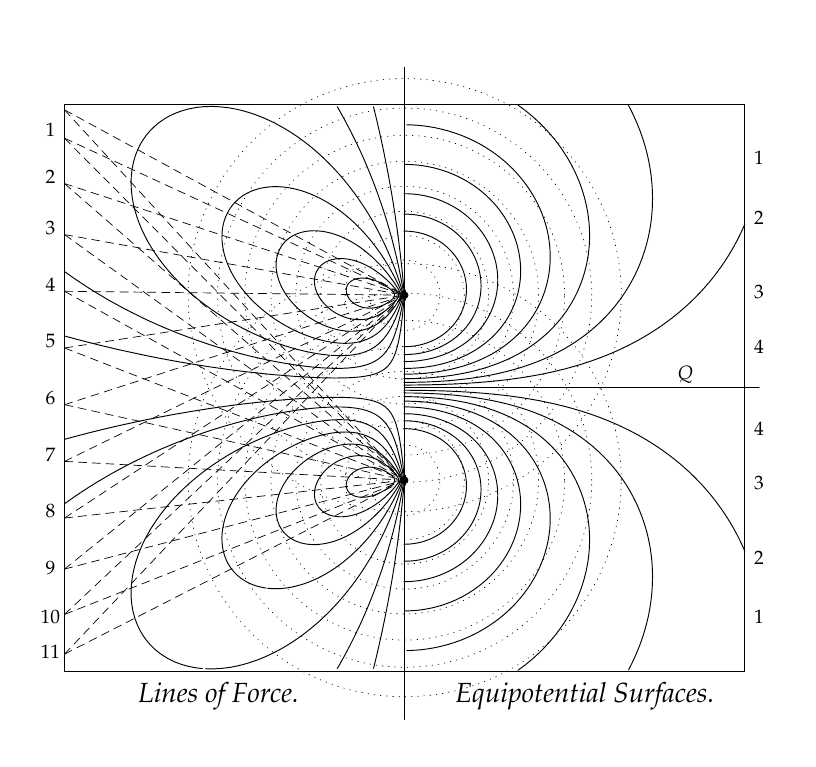
\begin{tikzpicture}[x=0.72cm,y=0.72cm,line cap=round,line join=round]
  \clip (-0.65,-1.20) rectangle (12.75,11.35);
  \draw[line width=0.45pt] (0,0) rectangle (12,10);
  \draw[line width=0.45pt] (6,-0.85) -- (6,10.65);
  \draw[line width=0.36pt] (6,5) -- (12.25,5);
  \draw[dotted,line width=0.25pt] (6.000,6.632) circle[radius=0.620];
  \draw[dotted,line width=0.25pt] (6.000,6.632) circle[radius=1.050];
  \draw[dotted,line width=0.25pt] (6.000,6.632) circle[radius=1.480];
  \draw[dotted,line width=0.25pt] (6.000,6.632) circle[radius=1.920];
  \draw[dotted,line width=0.25pt] (6.000,6.632) circle[radius=2.360];
  \draw[dotted,line width=0.25pt] (6.000,6.632) circle[radius=2.820];
  \draw[dotted,line width=0.25pt] (6.000,6.632) circle[radius=3.300];
  \draw[dotted,line width=0.25pt] (6.000,6.632) circle[radius=3.820];
  \draw[dotted,line width=0.25pt] (6.000,3.368) circle[radius=0.620];
  \draw[dotted,line width=0.25pt] (6.000,3.368) circle[radius=1.050];
  \draw[dotted,line width=0.25pt] (6.000,3.368) circle[radius=1.480];
  \draw[dotted,line width=0.25pt] (6.000,3.368) circle[radius=1.920];
  \draw[dotted,line width=0.25pt] (6.000,3.368) circle[radius=2.360];
  \draw[dotted,line width=0.25pt] (6.000,3.368) circle[radius=2.820];
  \draw[dotted,line width=0.25pt] (6.000,3.368) circle[radius=3.300];
  \draw[dotted,line width=0.25pt] (6.000,3.368) circle[radius=3.820];
  \draw[densely dashed,line width=0.25pt] (0,0.300) -- (6,6.632);
  \draw[densely dashed,line width=0.25pt] (0,1.000) -- (6,6.632);
  \draw[densely dashed,line width=0.25pt] (0,1.800) -- (6,6.632);
  \draw[densely dashed,line width=0.25pt] (0,2.700) -- (6,6.632);
  \draw[densely dashed,line width=0.25pt] (0,3.700) -- (6,6.632);
  \draw[densely dashed,line width=0.25pt] (0,4.700) -- (6,6.632);
  \draw[densely dashed,line width=0.25pt] (0,5.700) -- (6,6.632);
  \draw[densely dashed,line width=0.25pt] (0,6.700) -- (6,6.632);
  \draw[densely dashed,line width=0.25pt] (0,7.700) -- (6,6.632);
  \draw[densely dashed,line width=0.25pt] (0,8.600) -- (6,6.632);
  \draw[densely dashed,line width=0.25pt] (0,9.400) -- (6,6.632);
  \draw[densely dashed,line width=0.25pt] (0,9.900) -- (6,6.632);
  \draw[densely dashed,line width=0.25pt] (0,0.300) -- (6,3.368);
  \draw[densely dashed,line width=0.25pt] (0,1.000) -- (6,3.368);
  \draw[densely dashed,line width=0.25pt] (0,1.800) -- (6,3.368);
  \draw[densely dashed,line width=0.25pt] (0,2.700) -- (6,3.368);
  \draw[densely dashed,line width=0.25pt] (0,3.700) -- (6,3.368);
  \draw[densely dashed,line width=0.25pt] (0,4.700) -- (6,3.368);
  \draw[densely dashed,line width=0.25pt] (0,5.700) -- (6,3.368);
  \draw[densely dashed,line width=0.25pt] (0,6.700) -- (6,3.368);
  \draw[densely dashed,line width=0.25pt] (0,7.700) -- (6,3.368);
  \draw[densely dashed,line width=0.25pt] (0,8.600) -- (6,3.368);
  \draw[densely dashed,line width=0.25pt] (0,9.400) -- (6,3.368);
  \draw[densely dashed,line width=0.25pt] (0,9.900) -- (6,3.368);
% Lines of force, left panel.
  \draw[line width=0.34pt] (5.176,3.073) -- (5.159,3.077) -- (5.150,3.079) -- (5.124,3.087) -- (5.098,3.097) -- (5.091,3.100) -- (5.072,3.111) -- (5.052,3.124) -- (5.046,3.128) -- (5.025,3.147) -- (5.020,3.152) -- (5.005,3.170) -- (4.993,3.188) -- (4.990,3.193) -- (4.980,3.217) -- (4.974,3.240) -- (4.970,3.263) -- (4.969,3.287) -- (4.971,3.310) -- (4.975,3.333) -- (4.982,3.357) -- (4.992,3.380) -- (4.993,3.384) -- (5.004,3.403) -- (5.018,3.427) -- (5.020,3.428) -- (5.036,3.450) -- (5.046,3.460) -- (5.058,3.473) -- (5.072,3.486) -- (5.084,3.497) -- (5.098,3.507) -- (5.115,3.520) -- (5.124,3.526) -- (5.150,3.541) -- (5.154,3.543) -- (5.176,3.554) -- (5.203,3.565) -- (5.206,3.566) -- (5.229,3.574) -- (5.255,3.582) -- (5.281,3.588) -- (5.292,3.590) -- (5.307,3.592) -- (5.333,3.595) -- (5.359,3.597) -- (5.386,3.597) -- (5.412,3.597) -- (5.438,3.594) -- (5.464,3.591) -- (5.472,3.590) -- (5.490,3.586) -- (5.516,3.580) -- (5.542,3.573) -- (5.564,3.566) -- (5.569,3.565) -- (5.595,3.555) -- (5.621,3.544) -- (5.623,3.543) -- (5.647,3.531) -- (5.669,3.520) -- (5.673,3.518) -- (5.699,3.502) -- (5.708,3.497) -- (5.725,3.485) -- (5.741,3.473) -- (5.752,3.466) -- (5.770,3.450) -- (5.778,3.443) -- (5.794,3.427) -- (5.804,3.415) -- (5.812,3.403) -- (5.822,3.380) -- (5.823,3.357) -- (5.813,3.333) -- (5.804,3.320) -- (5.796,3.310) -- (5.778,3.290) -- (5.775,3.287) -- (5.752,3.266) -- (5.748,3.263) -- (5.725,3.245) -- (5.719,3.240) -- (5.699,3.226) -- (5.686,3.217) -- (5.673,3.208) -- (5.650,3.193) -- (5.647,3.191) -- (5.621,3.176) -- (5.610,3.170) -- (5.595,3.162) -- (5.569,3.148) -- (5.565,3.147) -- (5.542,3.136) -- (5.516,3.125) -- (5.513,3.124) -- (5.490,3.114) -- (5.464,3.105) -- (5.449,3.100) -- (5.438,3.096) -- (5.412,3.089) -- (5.386,3.083) -- (5.359,3.077) -- (5.358,3.077) -- (5.333,3.073) -- (5.307,3.070) -- (5.281,3.068) -- (5.255,3.067) -- (5.229,3.068) -- (5.203,3.070) -- (5.176,3.073);
  \draw[line width=0.34pt] (4.810,2.726) -- (4.796,2.727) -- (4.784,2.729) -- (4.758,2.733) -- (4.732,2.738) -- (4.706,2.745) -- (4.687,2.751) -- (4.680,2.753) -- (4.654,2.763) -- (4.628,2.774) -- (4.627,2.774) -- (4.601,2.788) -- (4.586,2.797) -- (4.575,2.804) -- (4.552,2.821) -- (4.549,2.823) -- (4.525,2.844) -- (4.523,2.846) -- (4.502,2.867) -- (4.497,2.873) -- (4.483,2.890) -- (4.471,2.908) -- (4.467,2.914) -- (4.453,2.937) -- (4.444,2.954) -- (4.441,2.960) -- (4.432,2.984) -- (4.424,3.007) -- (4.418,3.030) -- (4.418,3.030) -- (4.414,3.054) -- (4.411,3.077) -- (4.409,3.100) -- (4.408,3.124) -- (4.409,3.147) -- (4.411,3.170) -- (4.414,3.193) -- (4.418,3.216) -- (4.418,3.217) -- (4.424,3.240) -- (4.430,3.263) -- (4.438,3.287) -- (4.444,3.303) -- (4.447,3.310) -- (4.457,3.333) -- (4.468,3.357) -- (4.471,3.362) -- (4.480,3.380) -- (4.494,3.403) -- (4.497,3.408) -- (4.508,3.427) -- (4.523,3.448) -- (4.524,3.450) -- (4.542,3.473) -- (4.549,3.482) -- (4.561,3.497) -- (4.575,3.513) -- (4.581,3.520) -- (4.601,3.541) -- (4.603,3.543) -- (4.627,3.566) -- (4.627,3.567) -- (4.653,3.590) -- (4.654,3.590) -- (4.680,3.612) -- (4.681,3.613) -- (4.706,3.632) -- (4.712,3.636) -- (4.732,3.650) -- (4.746,3.660) -- (4.758,3.668) -- (4.783,3.683) -- (4.784,3.683) -- (4.810,3.698) -- (4.826,3.706) -- (4.837,3.712) -- (4.863,3.724) -- (4.875,3.730) -- (4.889,3.736) -- (4.915,3.746) -- (4.933,3.753) -- (4.941,3.756) -- (4.967,3.764) -- (4.993,3.772) -- (5.010,3.776) -- (5.020,3.778) -- (5.046,3.784) -- (5.072,3.789) -- (5.098,3.793) -- (5.124,3.796) -- (5.150,3.799) -- (5.170,3.800) -- (5.176,3.800) -- (5.203,3.800) -- (5.229,3.800) -- (5.233,3.800) -- (5.255,3.798) -- (5.281,3.796) -- (5.307,3.793) -- (5.333,3.788) -- (5.359,3.783) -- (5.386,3.777) -- (5.387,3.776) -- (5.412,3.769) -- (5.438,3.761) -- (5.459,3.753) -- (5.464,3.751) -- (5.490,3.741) -- (5.515,3.730) -- (5.516,3.729) -- (5.542,3.716) -- (5.560,3.706) -- (5.569,3.702) -- (5.595,3.686) -- (5.600,3.683) -- (5.621,3.670) -- (5.635,3.660) -- (5.647,3.652) -- (5.668,3.636) -- (5.673,3.632) -- (5.697,3.613) -- (5.699,3.612) -- (5.725,3.590) -- (5.725,3.589) -- (5.751,3.566) -- (5.752,3.566) -- (5.775,3.543) -- (5.778,3.540) -- (5.797,3.520) -- (5.804,3.513) -- (5.818,3.497) -- (5.830,3.484) -- (5.838,3.473) -- (5.856,3.452) -- (5.857,3.450) -- (5.873,3.427) -- (5.882,3.412) -- (5.887,3.403) -- (5.894,3.380) -- (5.894,3.357) -- (5.887,3.333) -- (5.882,3.324) -- (5.874,3.310) -- (5.858,3.287) -- (5.856,3.284) -- (5.840,3.263) -- (5.830,3.250) -- (5.821,3.240) -- (5.804,3.220) -- (5.801,3.217) -- (5.780,3.193) -- (5.778,3.190) -- (5.758,3.170) -- (5.752,3.163) -- (5.735,3.147) -- (5.725,3.136) -- (5.712,3.124) -- (5.699,3.111) -- (5.687,3.100) -- (5.673,3.087) -- (5.662,3.077) -- (5.647,3.063) -- (5.635,3.054) -- (5.621,3.041) -- (5.608,3.030) -- (5.595,3.019) -- (5.579,3.007) -- (5.569,2.999) -- (5.549,2.984) -- (5.542,2.979) -- (5.517,2.960) -- (5.516,2.960) -- (5.490,2.941) -- (5.484,2.937) -- (5.464,2.924) -- (5.448,2.914) -- (5.438,2.907) -- (5.412,2.891) -- (5.411,2.890) -- (5.386,2.876) -- (5.370,2.867) -- (5.359,2.861) -- (5.333,2.847) -- (5.327,2.844) -- (5.307,2.834) -- (5.281,2.822) -- (5.279,2.821) -- (5.255,2.810) -- (5.229,2.799) -- (5.225,2.797) -- (5.203,2.788) -- (5.176,2.779) -- (5.162,2.774) -- (5.150,2.770) -- (5.124,2.762) -- (5.098,2.754) -- (5.083,2.751) -- (5.072,2.748) -- (5.046,2.742) -- (5.020,2.737) -- (4.993,2.732) -- (4.967,2.729) -- (4.954,2.727) -- (4.941,2.726) -- (4.915,2.724) -- (4.889,2.723) -- (4.863,2.723) -- (4.837,2.724) -- (4.810,2.726);
  \draw[line width=0.34pt] (4.314,2.236) -- (4.288,2.239) -- (4.235,2.247) -- (4.183,2.259) -- (4.157,2.266) -- (4.105,2.284) -- (4.078,2.295) -- (4.052,2.308) -- (4.009,2.331) -- (3.974,2.354) -- (3.948,2.373) -- (3.922,2.395) -- (3.895,2.420) -- (3.870,2.448) -- (3.851,2.471) -- (3.834,2.494) -- (3.817,2.520) -- (3.793,2.564) -- (3.782,2.587) -- (3.765,2.632) -- (3.757,2.657) -- (3.745,2.704) -- (3.739,2.741) -- (3.735,2.774) -- (3.732,2.821) -- (3.732,2.867) -- (3.736,2.914) -- (3.739,2.937) -- (3.746,2.984) -- (3.757,3.030) -- (3.765,3.059) -- (3.778,3.100) -- (3.791,3.137) -- (3.804,3.170) -- (3.817,3.199) -- (3.837,3.240) -- (3.849,3.263) -- (3.869,3.298) -- (3.891,3.333) -- (3.906,3.357) -- (3.922,3.380) -- (3.948,3.416) -- (3.974,3.449) -- (3.993,3.473) -- (4.014,3.497) -- (4.034,3.520) -- (4.056,3.543) -- (4.079,3.566) -- (4.105,3.591) -- (4.131,3.615) -- (4.157,3.639) -- (4.183,3.661) -- (4.211,3.683) -- (4.241,3.706) -- (4.272,3.730) -- (4.306,3.753) -- (4.340,3.775) -- (4.366,3.792) -- (4.392,3.807) -- (4.419,3.823) -- (4.462,3.846) -- (4.497,3.864) -- (4.523,3.876) -- (4.559,3.893) -- (4.601,3.910) -- (4.627,3.921) -- (4.680,3.939) -- (4.706,3.948) -- (4.756,3.963) -- (4.784,3.970) -- (4.837,3.982) -- (4.863,3.987) -- (4.915,3.995) -- (4.967,4.001) -- (5.020,4.005) -- (5.072,4.005) -- (5.124,4.003) -- (5.176,3.998) -- (5.229,3.990) -- (5.255,3.985) -- (5.307,3.971) -- (5.334,3.963) -- (5.386,3.944) -- (5.412,3.932) -- (5.445,3.916) -- (5.488,3.893) -- (5.516,3.876) -- (5.542,3.858) -- (5.569,3.840) -- (5.595,3.819) -- (5.621,3.798) -- (5.647,3.774) -- (5.673,3.750) -- (5.699,3.723) -- (5.725,3.695) -- (5.752,3.665) -- (5.775,3.636) -- (5.793,3.613) -- (5.810,3.590) -- (5.830,3.563) -- (5.856,3.524) -- (5.874,3.497) -- (5.888,3.473) -- (5.908,3.438) -- (5.924,3.403) -- (5.932,3.357) -- (5.914,3.310) -- (5.902,3.287) -- (5.882,3.252) -- (5.860,3.217) -- (5.845,3.193) -- (5.830,3.169) -- (5.804,3.130) -- (5.782,3.100) -- (5.765,3.077) -- (5.748,3.054) -- (5.725,3.023) -- (5.699,2.989) -- (5.676,2.960) -- (5.656,2.937) -- (5.637,2.914) -- (5.617,2.890) -- (5.595,2.866) -- (5.569,2.837) -- (5.542,2.809) -- (5.516,2.782) -- (5.490,2.756) -- (5.464,2.731) -- (5.438,2.707) -- (5.412,2.683) -- (5.386,2.660) -- (5.359,2.637) -- (5.333,2.616) -- (5.307,2.595) -- (5.281,2.574) -- (5.255,2.554) -- (5.229,2.535) -- (5.203,2.517) -- (5.169,2.494) -- (5.133,2.471) -- (5.098,2.449) -- (5.072,2.434) -- (5.046,2.419) -- (5.013,2.401) -- (4.968,2.378) -- (4.941,2.365) -- (4.915,2.353) -- (4.864,2.331) -- (4.837,2.320) -- (4.804,2.308) -- (4.758,2.292) -- (4.732,2.284) -- (4.680,2.269) -- (4.645,2.261) -- (4.601,2.252) -- (4.549,2.243) -- (4.506,2.238) -- (4.471,2.235) -- (4.418,2.232) -- (4.366,2.233) -- (4.314,2.236);
  \draw[line width=0.34pt] (3.556,1.465) -- (3.503,1.474) -- (3.425,1.491) -- (3.373,1.506) -- (3.320,1.525) -- (3.268,1.547) -- (3.216,1.573) -- (3.163,1.603) -- (3.121,1.632) -- (3.085,1.659) -- (3.036,1.702) -- (3.007,1.731) -- (2.971,1.772) -- (2.935,1.818) -- (2.904,1.865) -- (2.877,1.911) -- (2.854,1.958) -- (2.835,2.005) -- (2.819,2.051) -- (2.800,2.121) -- (2.791,2.168) -- (2.781,2.238) -- (2.777,2.308) -- (2.777,2.378) -- (2.782,2.448) -- (2.791,2.517) -- (2.799,2.564) -- (2.815,2.634) -- (2.828,2.681) -- (2.850,2.748) -- (2.868,2.797) -- (2.886,2.844) -- (2.907,2.890) -- (2.929,2.937) -- (2.954,2.985) -- (2.980,3.032) -- (3.007,3.077) -- (3.037,3.124) -- (3.068,3.170) -- (3.102,3.217) -- (3.137,3.263) -- (3.163,3.296) -- (3.194,3.333) -- (3.235,3.380) -- (3.268,3.416) -- (3.301,3.450) -- (3.346,3.496) -- (3.373,3.521) -- (3.422,3.566) -- (3.451,3.592) -- (3.503,3.636) -- (3.533,3.660) -- (3.582,3.698) -- (3.624,3.730) -- (3.660,3.755) -- (3.712,3.791) -- (3.761,3.823) -- (3.798,3.846) -- (3.843,3.874) -- (3.895,3.904) -- (3.948,3.933) -- (4.000,3.960) -- (4.052,3.986) -- (4.102,4.009) -- (4.154,4.033) -- (4.209,4.056) -- (4.261,4.076) -- (4.314,4.096) -- (4.366,4.114) -- (4.418,4.130) -- (4.483,4.149) -- (4.549,4.166) -- (4.601,4.178) -- (4.680,4.193) -- (4.732,4.202) -- (4.810,4.211) -- (4.889,4.216) -- (4.967,4.218) -- (5.046,4.214) -- (5.124,4.205) -- (5.176,4.196) -- (5.255,4.176) -- (5.307,4.158) -- (5.359,4.137) -- (5.412,4.111) -- (5.464,4.080) -- (5.499,4.056) -- (5.542,4.023) -- (5.584,3.986) -- (5.621,3.950) -- (5.652,3.916) -- (5.691,3.869) -- (5.725,3.825) -- (5.752,3.787) -- (5.778,3.747) -- (5.804,3.705) -- (5.830,3.659) -- (5.856,3.611) -- (5.882,3.559) -- (5.908,3.504) -- (5.932,3.450) -- (5.949,3.403) -- (5.949,3.333) -- (5.932,3.287) -- (5.908,3.231) -- (5.882,3.174) -- (5.858,3.124) -- (5.835,3.077) -- (5.811,3.030) -- (5.786,2.984) -- (5.760,2.937) -- (5.734,2.890) -- (5.707,2.844) -- (5.679,2.797) -- (5.650,2.751) -- (5.621,2.706) -- (5.595,2.666) -- (5.569,2.628) -- (5.540,2.587) -- (5.506,2.541) -- (5.471,2.494) -- (5.438,2.451) -- (5.412,2.418) -- (5.379,2.378) -- (5.339,2.331) -- (5.307,2.294) -- (5.277,2.261) -- (5.234,2.214) -- (5.203,2.182) -- (5.165,2.145) -- (5.124,2.105) -- (5.092,2.075) -- (5.046,2.033) -- (5.013,2.005) -- (4.967,1.966) -- (4.929,1.935) -- (4.889,1.903) -- (4.838,1.865) -- (4.805,1.841) -- (4.758,1.809) -- (4.706,1.775) -- (4.664,1.748) -- (4.625,1.725) -- (4.575,1.697) -- (4.523,1.669) -- (4.471,1.642) -- (4.418,1.618) -- (4.366,1.595) -- (4.314,1.573) -- (4.261,1.554) -- (4.209,1.536) -- (4.141,1.515) -- (4.078,1.499) -- (4.026,1.487) -- (3.948,1.472) -- (3.895,1.465) -- (3.817,1.457) -- (3.739,1.454) -- (3.660,1.455) -- (3.582,1.462);
  \draw[line width=0.34pt] (2.431,0.045) -- (2.301,0.061) -- (2.170,0.088) -- (2.065,0.118) -- (1.945,0.163) -- (1.847,0.210) -- (1.752,0.266) -- (1.665,0.326) -- (1.582,0.396) -- (1.511,0.466) -- (1.438,0.553) -- (1.384,0.629) -- (1.329,0.723) -- (1.281,0.825) -- (1.241,0.932) -- (1.209,1.049) -- (1.188,1.166) -- (1.176,1.284) -- (1.174,1.422) -- (1.181,1.538) -- (1.199,1.678) -- (1.223,1.795) -- (1.253,1.911) -- (1.283,2.005) -- (1.326,2.121) -- (1.366,2.214) -- (1.412,2.312) -- (1.464,2.411) -- (1.516,2.502) -- (1.570,2.587) -- (1.633,2.681) -- (1.699,2.772) -- (1.755,2.844) -- (1.830,2.935) -- (1.893,3.007) -- (1.961,3.080) -- (2.039,3.160) -- (2.118,3.236) -- (2.196,3.307) -- (2.275,3.375) -- (2.353,3.440) -- (2.431,3.502) -- (2.517,3.566) -- (2.614,3.635) -- (2.693,3.688) -- (2.793,3.753) -- (2.876,3.804) -- (2.980,3.864) -- (3.075,3.916) -- (3.164,3.963) -- (3.268,4.014) -- (3.373,4.063) -- (3.477,4.108) -- (3.582,4.151) -- (3.698,4.196) -- (3.817,4.238) -- (3.922,4.272) -- (4.052,4.310) -- (4.157,4.338) -- (4.288,4.368) -- (4.418,4.393) -- (4.549,4.414) -- (4.691,4.429) -- (4.837,4.436) -- (4.993,4.432) -- (5.124,4.416) -- (5.255,4.385) -- (5.359,4.345) -- (5.461,4.289) -- (5.542,4.227) -- (5.620,4.149) -- (5.676,4.079) -- (5.737,3.986) -- (5.787,3.893) -- (5.831,3.800) -- (5.878,3.683) -- (5.911,3.590) -- (5.948,3.473) -- (5.971,3.357) -- (5.941,3.240) -- (5.908,3.135) -- (5.873,3.030) -- (5.831,2.914) -- (5.796,2.821) -- (5.752,2.710) -- (5.710,2.611) -- (5.668,2.517) -- (5.621,2.417) -- (5.569,2.311) -- (5.519,2.214) -- (5.468,2.121) -- (5.415,2.028) -- (5.359,1.936) -- (5.307,1.852) -- (5.255,1.771) -- (5.192,1.678) -- (5.125,1.585) -- (5.072,1.513) -- (5.001,1.422) -- (4.941,1.348) -- (4.865,1.259) -- (4.803,1.189) -- (4.732,1.113) -- (4.654,1.032) -- (4.575,0.956) -- (4.500,0.886) -- (4.420,0.816) -- (4.340,0.749) -- (4.261,0.686) -- (4.183,0.627) -- (4.087,0.559) -- (4.000,0.501) -- (3.906,0.443) -- (3.817,0.391) -- (3.712,0.335) -- (3.608,0.284) -- (3.503,0.238) -- (3.399,0.196) -- (3.294,0.160) -- (3.163,0.120) -- (3.055,0.093) -- (2.928,0.068) -- (2.771,0.048) -- (2.641,0.040) -- (2.484,0.042);
  \draw[line width=0.34pt] (0.000,2.952) -- (0.052,2.989) -- (0.110,3.030) -- (0.177,3.077) -- (0.235,3.116) -- (0.288,3.152) -- (0.351,3.193) -- (0.418,3.237) -- (0.471,3.270) -- (0.535,3.310) -- (0.601,3.350) -- (0.654,3.381) -- (0.730,3.427) -- (0.784,3.458) -- (0.853,3.497) -- (0.915,3.531) -- (0.980,3.566) -- (1.046,3.601) -- (1.113,3.636) -- (1.176,3.669) -- (1.251,3.706) -- (1.307,3.734) -- (1.386,3.772) -- (1.444,3.800) -- (1.516,3.833) -- (1.595,3.869) -- (1.649,3.893) -- (1.725,3.926) -- (1.804,3.959) -- (1.869,3.986) -- (1.935,4.013) -- (2.013,4.044) -- (2.092,4.074) -- (2.166,4.103) -- (2.229,4.126) -- (2.301,4.152) -- (2.379,4.179) -- (2.458,4.206) -- (2.536,4.232) -- (2.614,4.258) -- (2.693,4.282) -- (2.771,4.306) -- (2.850,4.329) -- (2.928,4.352) -- (3.007,4.374) -- (3.085,4.395) -- (3.163,4.415) -- (3.242,4.435) -- (3.320,4.454) -- (3.413,4.476) -- (3.503,4.495) -- (3.582,4.512) -- (3.660,4.528) -- (3.751,4.545) -- (3.843,4.562) -- (3.922,4.575) -- (4.026,4.592) -- (4.105,4.604) -- (4.193,4.615) -- (4.288,4.627) -- (4.392,4.638) -- (4.471,4.645) -- (4.575,4.652) -- (4.680,4.657) -- (4.784,4.660) -- (4.889,4.659) -- (4.993,4.654) -- (5.098,4.644) -- (5.176,4.633) -- (5.262,4.615) -- (5.343,4.592) -- (5.412,4.565) -- (5.490,4.525) -- (5.542,4.490) -- (5.595,4.447) -- (5.647,4.393) -- (5.691,4.336) -- (5.725,4.282) -- (5.760,4.219) -- (5.792,4.149) -- (5.820,4.079) -- (5.844,4.009) -- (5.866,3.939) -- (5.885,3.869) -- (5.908,3.777) -- (5.924,3.706) -- (5.939,3.636) -- (5.957,3.543) -- (5.970,3.473) -- (5.985,3.380) -- (5.974,3.287) -- (5.961,3.210) -- (5.945,3.124) -- (5.931,3.054) -- (5.912,2.960) -- (5.898,2.890) -- (5.882,2.819) -- (5.862,2.727) -- (5.845,2.657) -- (5.828,2.587) -- (5.805,2.494) -- (5.787,2.424) -- (5.768,2.354) -- (5.749,2.284) -- (5.725,2.201) -- (5.702,2.121) -- (5.681,2.051) -- (5.659,1.981) -- (5.637,1.911) -- (5.614,1.841) -- (5.591,1.772) -- (5.567,1.702) -- (5.542,1.631) -- (5.516,1.558) -- (5.490,1.487) -- (5.464,1.417) -- (5.438,1.350) -- (5.411,1.282) -- (5.383,1.212) -- (5.354,1.142) -- (5.325,1.072) -- (5.295,1.002) -- (5.264,0.932) -- (5.233,0.862) -- (5.203,0.797) -- (5.176,0.741) -- (5.145,0.676) -- (5.111,0.606) -- (5.076,0.536) -- (5.046,0.475) -- (5.017,0.420) -- (4.980,0.350) -- (4.943,0.280) -- (4.915,0.229) -- (4.878,0.163) -- (4.839,0.093) -- (4.810,0.045);
  \draw[line width=0.34pt] (0.000,4.088) -- (0.078,4.110) -- (0.157,4.131) -- (0.235,4.152) -- (0.314,4.172) -- (0.404,4.196) -- (0.496,4.219) -- (0.575,4.239) -- (0.654,4.258) -- (0.732,4.277) -- (0.810,4.295) -- (0.889,4.314) -- (0.985,4.336) -- (1.072,4.355) -- (1.150,4.372) -- (1.229,4.389) -- (1.307,4.406) -- (1.412,4.428) -- (1.490,4.444) -- (1.569,4.460) -- (1.650,4.476) -- (1.752,4.495) -- (1.830,4.510) -- (1.908,4.524) -- (2.013,4.543) -- (2.092,4.556) -- (2.170,4.570) -- (2.275,4.587) -- (2.353,4.600) -- (2.450,4.615) -- (2.536,4.629) -- (2.614,4.640) -- (2.719,4.655) -- (2.797,4.666) -- (2.902,4.681) -- (2.980,4.691) -- (3.085,4.704) -- (3.163,4.714) -- (3.268,4.726) -- (3.346,4.735) -- (3.451,4.746) -- (3.536,4.755) -- (3.634,4.765) -- (3.739,4.775) -- (3.817,4.781) -- (3.922,4.790) -- (4.026,4.798) -- (4.105,4.803) -- (4.209,4.810) -- (4.314,4.816) -- (4.418,4.821) -- (4.523,4.825) -- (4.601,4.827) -- (4.706,4.829) -- (4.810,4.829) -- (4.915,4.828) -- (5.010,4.825) -- (5.098,4.820) -- (5.203,4.811) -- (5.281,4.801) -- (5.386,4.782) -- (5.464,4.761) -- (5.542,4.732) -- (5.595,4.705) -- (5.658,4.662) -- (5.708,4.615) -- (5.752,4.560) -- (5.788,4.499) -- (5.821,4.429) -- (5.846,4.359) -- (5.867,4.289) -- (5.884,4.219) -- (5.904,4.126) -- (5.916,4.056) -- (5.931,3.963) -- (5.941,3.893) -- (5.952,3.800) -- (5.961,3.726) -- (5.970,3.636) -- (5.979,3.543) -- (5.987,3.456) -- (5.993,3.380) -- (5.987,3.287) -- (5.981,3.217) -- (5.973,3.124) -- (5.964,3.030) -- (5.957,2.960) -- (5.947,2.867) -- (5.937,2.774) -- (5.929,2.704) -- (5.919,2.611) -- (5.908,2.527) -- (5.899,2.448) -- (5.887,2.354) -- (5.877,2.284) -- (5.865,2.191) -- (5.855,2.121) -- (5.841,2.028) -- (5.830,1.953) -- (5.817,1.865) -- (5.804,1.784) -- (5.791,1.702) -- (5.778,1.624) -- (5.763,1.538) -- (5.751,1.469) -- (5.735,1.375) -- (5.722,1.305) -- (5.705,1.212) -- (5.691,1.142) -- (5.673,1.049) -- (5.659,0.979) -- (5.645,0.909) -- (5.626,0.816) -- (5.611,0.746) -- (5.595,0.669) -- (5.576,0.583) -- (5.560,0.513) -- (5.542,0.434) -- (5.523,0.350) -- (5.507,0.280) -- (5.490,0.210) -- (5.467,0.117) -- (5.450,0.047);
  \draw[line width=0.34pt] (6.013,6.544) -- (6.013,6.550) -- (6.011,6.573) -- (6.009,6.597) -- (6.007,6.620) -- (6.007,6.643) -- (6.009,6.667) -- (6.011,6.690) -- (6.013,6.713) -- (6.013,6.719);
  \draw[line width=0.34pt] (6.013,3.456) -- (6.013,3.450) -- (6.011,3.427) -- (6.009,3.403) -- (6.007,3.380) -- (6.007,3.357) -- (6.009,3.333) -- (6.011,3.310) -- (6.013,3.287) -- (6.013,3.281);
  \draw[line width=0.34pt] (0.000,5.912) -- (0.078,5.890) -- (0.157,5.869) -- (0.235,5.848) -- (0.314,5.828) -- (0.404,5.804) -- (0.496,5.781) -- (0.575,5.761) -- (0.654,5.742) -- (0.732,5.723) -- (0.810,5.705) -- (0.889,5.686) -- (0.985,5.664) -- (1.072,5.645) -- (1.150,5.628) -- (1.229,5.611) -- (1.307,5.594) -- (1.412,5.572) -- (1.490,5.556) -- (1.569,5.540) -- (1.650,5.524) -- (1.752,5.505) -- (1.830,5.490) -- (1.908,5.476) -- (2.013,5.457) -- (2.092,5.444) -- (2.170,5.430) -- (2.275,5.413) -- (2.353,5.400) -- (2.450,5.385) -- (2.536,5.371) -- (2.614,5.360) -- (2.719,5.345) -- (2.797,5.334) -- (2.902,5.319) -- (2.980,5.309) -- (3.085,5.296) -- (3.163,5.286) -- (3.268,5.274) -- (3.346,5.265) -- (3.451,5.254) -- (3.536,5.245) -- (3.634,5.235) -- (3.739,5.225) -- (3.817,5.219) -- (3.922,5.210) -- (4.026,5.202) -- (4.105,5.197) -- (4.209,5.190) -- (4.314,5.184) -- (4.418,5.179) -- (4.523,5.175) -- (4.601,5.173) -- (4.706,5.171) -- (4.810,5.171) -- (4.915,5.172) -- (5.010,5.175) -- (5.098,5.180) -- (5.203,5.189) -- (5.281,5.199) -- (5.386,5.218) -- (5.464,5.239) -- (5.542,5.268) -- (5.595,5.295) -- (5.658,5.338) -- (5.708,5.385) -- (5.752,5.440) -- (5.788,5.501) -- (5.821,5.571) -- (5.846,5.641) -- (5.867,5.711) -- (5.884,5.781) -- (5.904,5.874) -- (5.916,5.944) -- (5.931,6.037) -- (5.941,6.107) -- (5.952,6.200) -- (5.961,6.274) -- (5.970,6.364) -- (5.979,6.457) -- (5.987,6.544) -- (5.993,6.620) -- (5.987,6.713) -- (5.981,6.783) -- (5.973,6.876) -- (5.964,6.970) -- (5.957,7.040) -- (5.947,7.133) -- (5.937,7.226) -- (5.929,7.296) -- (5.919,7.389) -- (5.908,7.473) -- (5.899,7.552) -- (5.887,7.646) -- (5.877,7.716) -- (5.865,7.809) -- (5.855,7.879) -- (5.841,7.972) -- (5.830,8.047) -- (5.817,8.135) -- (5.804,8.216) -- (5.791,8.298) -- (5.778,8.376) -- (5.763,8.462) -- (5.751,8.531) -- (5.735,8.625) -- (5.722,8.695) -- (5.705,8.788) -- (5.691,8.858) -- (5.673,8.951) -- (5.659,9.021) -- (5.645,9.091) -- (5.626,9.184) -- (5.611,9.254) -- (5.595,9.331) -- (5.576,9.417) -- (5.560,9.487) -- (5.542,9.566) -- (5.523,9.650) -- (5.507,9.720) -- (5.490,9.790) -- (5.467,9.883) -- (5.450,9.953);
  \draw[line width=0.34pt] (0.000,7.048) -- (0.052,7.011) -- (0.110,6.970) -- (0.177,6.923) -- (0.235,6.884) -- (0.288,6.848) -- (0.351,6.807) -- (0.418,6.763) -- (0.471,6.730) -- (0.535,6.690) -- (0.601,6.650) -- (0.654,6.619) -- (0.730,6.573) -- (0.784,6.542) -- (0.853,6.503) -- (0.915,6.469) -- (0.980,6.434) -- (1.046,6.399) -- (1.113,6.364) -- (1.176,6.331) -- (1.251,6.294) -- (1.307,6.266) -- (1.386,6.228) -- (1.444,6.200) -- (1.516,6.167) -- (1.595,6.131) -- (1.649,6.107) -- (1.725,6.074) -- (1.804,6.041) -- (1.869,6.014) -- (1.935,5.987) -- (2.013,5.956) -- (2.092,5.926) -- (2.166,5.897) -- (2.229,5.874) -- (2.301,5.848) -- (2.379,5.821) -- (2.458,5.794) -- (2.536,5.768) -- (2.614,5.742) -- (2.693,5.718) -- (2.771,5.694) -- (2.850,5.671) -- (2.928,5.648) -- (3.007,5.626) -- (3.085,5.605) -- (3.163,5.585) -- (3.242,5.565) -- (3.320,5.546) -- (3.413,5.524) -- (3.503,5.505) -- (3.582,5.488) -- (3.660,5.472) -- (3.751,5.455) -- (3.843,5.438) -- (3.922,5.425) -- (4.026,5.408) -- (4.105,5.396) -- (4.193,5.385) -- (4.288,5.373) -- (4.392,5.362) -- (4.471,5.355) -- (4.575,5.348) -- (4.680,5.343) -- (4.784,5.340) -- (4.889,5.341) -- (4.993,5.346) -- (5.098,5.356) -- (5.176,5.367) -- (5.262,5.385) -- (5.343,5.408) -- (5.412,5.435) -- (5.490,5.475) -- (5.542,5.510) -- (5.595,5.553) -- (5.647,5.607) -- (5.691,5.664) -- (5.725,5.718) -- (5.760,5.781) -- (5.792,5.851) -- (5.820,5.921) -- (5.844,5.991) -- (5.866,6.061) -- (5.885,6.131) -- (5.908,6.223) -- (5.924,6.294) -- (5.939,6.364) -- (5.957,6.457) -- (5.970,6.527) -- (5.985,6.620) -- (5.974,6.713) -- (5.961,6.790) -- (5.945,6.876) -- (5.931,6.946) -- (5.912,7.040) -- (5.898,7.110) -- (5.882,7.181) -- (5.862,7.273) -- (5.845,7.343) -- (5.828,7.413) -- (5.805,7.506) -- (5.787,7.576) -- (5.768,7.646) -- (5.749,7.716) -- (5.725,7.799) -- (5.702,7.879) -- (5.681,7.949) -- (5.659,8.019) -- (5.637,8.089) -- (5.614,8.159) -- (5.591,8.228) -- (5.567,8.298) -- (5.542,8.369) -- (5.516,8.442) -- (5.490,8.513) -- (5.464,8.583) -- (5.438,8.650) -- (5.411,8.718) -- (5.383,8.788) -- (5.354,8.858) -- (5.325,8.928) -- (5.295,8.998) -- (5.264,9.068) -- (5.233,9.138) -- (5.203,9.203) -- (5.176,9.259) -- (5.145,9.324) -- (5.111,9.394) -- (5.076,9.464) -- (5.046,9.525) -- (5.017,9.580) -- (4.980,9.650) -- (4.943,9.720) -- (4.915,9.771) -- (4.878,9.837) -- (4.839,9.907) -- (4.810,9.955);
  \draw[line width=0.34pt] (4.706,5.570) -- (4.863,5.564) -- (5.020,5.570) -- (5.150,5.589) -- (5.263,5.618) -- (5.379,5.664) -- (5.464,5.713) -- (5.551,5.781) -- (5.621,5.851) -- (5.692,5.944) -- (5.750,6.037) -- (5.799,6.131) -- (5.841,6.224) -- (5.882,6.329) -- (5.918,6.434) -- (5.955,6.550) -- (5.967,6.667) -- (5.935,6.782) -- (5.904,6.876) -- (5.865,6.993) -- (5.830,7.090) -- (5.787,7.203) -- (5.749,7.296) -- (5.699,7.413) -- (5.657,7.506) -- (5.613,7.599) -- (5.567,7.692) -- (5.516,7.790) -- (5.464,7.886) -- (5.412,7.977) -- (5.359,8.065) -- (5.301,8.159) -- (5.239,8.252) -- (5.176,8.343) -- (5.124,8.416) -- (5.055,8.508) -- (4.993,8.587) -- (4.925,8.671) -- (4.863,8.744) -- (4.784,8.831) -- (4.716,8.904) -- (4.647,8.974) -- (4.575,9.044) -- (4.497,9.117) -- (4.418,9.186) -- (4.337,9.254) -- (4.248,9.324) -- (4.157,9.392) -- (4.078,9.447) -- (3.981,9.510) -- (3.895,9.563) -- (3.791,9.623) -- (3.695,9.674) -- (3.598,9.720) -- (3.492,9.767) -- (3.373,9.813) -- (3.268,9.849) -- (3.150,9.883) -- (3.033,9.912) -- (2.902,9.936) -- (2.756,9.953) -- (2.614,9.961) -- (2.458,9.957) -- (2.327,9.943) -- (2.196,9.918) -- (2.070,9.883) -- (1.961,9.843) -- (1.856,9.795) -- (1.766,9.744) -- (1.673,9.680) -- (1.595,9.616) -- (1.516,9.539) -- (1.451,9.464) -- (1.386,9.373) -- (1.333,9.285) -- (1.285,9.184) -- (1.249,9.091) -- (1.215,8.974) -- (1.192,8.858) -- (1.177,8.718) -- (1.174,8.601) -- (1.179,8.485) -- (1.195,8.345) -- (1.217,8.228) -- (1.246,8.112) -- (1.281,8.000) -- (1.317,7.902) -- (1.359,7.800) -- (1.410,7.692) -- (1.458,7.599) -- (1.512,7.506) -- (1.569,7.414) -- (1.621,7.336) -- (1.683,7.249) -- (1.752,7.160) -- (1.812,7.086) -- (1.882,7.005) -- (1.958,6.923) -- (2.026,6.853) -- (2.098,6.783) -- (2.173,6.713) -- (2.252,6.643) -- (2.336,6.573) -- (2.424,6.503) -- (2.510,6.439) -- (2.588,6.383) -- (2.684,6.317) -- (2.771,6.261) -- (2.869,6.200) -- (2.954,6.151) -- (3.059,6.092) -- (3.163,6.038) -- (3.258,5.991) -- (3.357,5.944) -- (3.463,5.897) -- (3.576,5.851) -- (3.686,5.809) -- (3.791,5.771) -- (3.903,5.734) -- (4.026,5.697) -- (4.149,5.664) -- (4.261,5.638) -- (4.392,5.611) -- (4.523,5.590) -- (4.680,5.572);
  \draw[line width=0.34pt] (4.706,5.802) -- (4.784,5.792) -- (4.863,5.785) -- (4.941,5.782) -- (5.020,5.784) -- (5.098,5.791) -- (5.176,5.804) -- (5.229,5.817) -- (5.281,5.832) -- (5.333,5.852) -- (5.386,5.876) -- (5.438,5.904) -- (5.490,5.938) -- (5.530,5.967) -- (5.569,6.000) -- (5.608,6.037) -- (5.647,6.078) -- (5.673,6.108) -- (5.709,6.154) -- (5.743,6.200) -- (5.774,6.247) -- (5.803,6.294) -- (5.830,6.340) -- (5.855,6.387) -- (5.878,6.434) -- (5.901,6.480) -- (5.921,6.527) -- (5.941,6.573) -- (5.956,6.643) -- (5.935,6.708) -- (5.912,6.760) -- (5.891,6.807) -- (5.869,6.853) -- (5.846,6.900) -- (5.823,6.946) -- (5.798,6.993) -- (5.773,7.040) -- (5.747,7.086) -- (5.721,7.133) -- (5.693,7.179) -- (5.664,7.226) -- (5.635,7.273) -- (5.604,7.319) -- (5.573,7.366) -- (5.542,7.409) -- (5.516,7.446) -- (5.489,7.483) -- (5.453,7.529) -- (5.417,7.576) -- (5.386,7.614) -- (5.359,7.646) -- (5.319,7.692) -- (5.281,7.735) -- (5.255,7.763) -- (5.211,7.809) -- (5.176,7.844) -- (5.141,7.879) -- (5.098,7.920) -- (5.066,7.949) -- (5.020,7.990) -- (4.986,8.019) -- (4.941,8.056) -- (4.899,8.089) -- (4.863,8.117) -- (4.810,8.155) -- (4.771,8.182) -- (4.732,8.208) -- (4.680,8.242) -- (4.627,8.273) -- (4.584,8.298) -- (4.541,8.322) -- (4.496,8.345) -- (4.444,8.370) -- (4.392,8.394) -- (4.340,8.416) -- (4.283,8.438) -- (4.217,8.462) -- (4.157,8.480) -- (4.105,8.495) -- (4.049,8.508) -- (3.974,8.523) -- (3.922,8.532) -- (3.843,8.541) -- (3.765,8.545) -- (3.686,8.546) -- (3.608,8.541) -- (3.532,8.531) -- (3.477,8.521) -- (3.422,8.508) -- (3.346,8.485) -- (3.294,8.465) -- (3.242,8.441) -- (3.194,8.415) -- (3.155,8.392) -- (3.111,8.361) -- (3.062,8.322) -- (3.033,8.295) -- (2.991,8.252) -- (2.954,8.208) -- (2.928,8.173) -- (2.902,8.132) -- (2.876,8.086) -- (2.850,8.031) -- (2.827,7.972) -- (2.812,7.925) -- (2.797,7.866) -- (2.787,7.809) -- (2.779,7.739) -- (2.777,7.669) -- (2.778,7.599) -- (2.785,7.529) -- (2.795,7.459) -- (2.804,7.413) -- (2.821,7.343) -- (2.835,7.296) -- (2.850,7.249) -- (2.876,7.182) -- (2.896,7.133) -- (2.918,7.086) -- (2.941,7.040) -- (2.966,6.993) -- (2.993,6.946) -- (3.022,6.900) -- (3.052,6.853) -- (3.085,6.807) -- (3.111,6.771) -- (3.137,6.736) -- (3.175,6.690) -- (3.214,6.643) -- (3.242,6.613) -- (3.278,6.573) -- (3.320,6.530) -- (3.347,6.503) -- (3.397,6.457) -- (3.425,6.431) -- (3.476,6.387) -- (3.504,6.364) -- (3.556,6.322) -- (3.593,6.294) -- (3.634,6.264) -- (3.686,6.227) -- (3.725,6.200) -- (3.765,6.175) -- (3.817,6.142) -- (3.869,6.111) -- (3.917,6.084) -- (3.960,6.061) -- (4.005,6.037) -- (4.052,6.014) -- (4.105,5.989) -- (4.157,5.966) -- (4.210,5.944) -- (4.269,5.921) -- (4.334,5.897) -- (4.392,5.878) -- (4.444,5.862) -- (4.497,5.847) -- (4.575,5.828) -- (4.627,5.817) -- (4.695,5.804);
  \draw[line width=0.34pt] (4.863,6.013) -- (4.915,6.005) -- (4.967,5.999) -- (5.020,5.995) -- (5.072,5.995) -- (5.124,5.997) -- (5.176,6.002) -- (5.229,6.010) -- (5.255,6.015) -- (5.307,6.029) -- (5.334,6.037) -- (5.386,6.056) -- (5.412,6.068) -- (5.445,6.084) -- (5.488,6.107) -- (5.516,6.124) -- (5.542,6.142) -- (5.569,6.160) -- (5.595,6.181) -- (5.621,6.202) -- (5.647,6.226) -- (5.673,6.250) -- (5.699,6.277) -- (5.725,6.305) -- (5.752,6.335) -- (5.775,6.364) -- (5.793,6.387) -- (5.810,6.410) -- (5.830,6.437) -- (5.856,6.476) -- (5.874,6.503) -- (5.888,6.527) -- (5.908,6.562) -- (5.924,6.597) -- (5.932,6.643) -- (5.914,6.690) -- (5.902,6.713) -- (5.882,6.748) -- (5.860,6.783) -- (5.845,6.807) -- (5.830,6.831) -- (5.804,6.870) -- (5.782,6.900) -- (5.765,6.923) -- (5.748,6.946) -- (5.725,6.977) -- (5.699,7.011) -- (5.676,7.040) -- (5.656,7.063) -- (5.637,7.086) -- (5.617,7.110) -- (5.595,7.134) -- (5.569,7.163) -- (5.542,7.191) -- (5.516,7.218) -- (5.490,7.244) -- (5.464,7.269) -- (5.438,7.293) -- (5.412,7.317) -- (5.386,7.340) -- (5.359,7.363) -- (5.333,7.384) -- (5.307,7.405) -- (5.281,7.426) -- (5.255,7.446) -- (5.229,7.465) -- (5.203,7.483) -- (5.169,7.506) -- (5.133,7.529) -- (5.098,7.551) -- (5.072,7.566) -- (5.046,7.581) -- (5.013,7.599) -- (4.968,7.622) -- (4.941,7.635) -- (4.915,7.647) -- (4.864,7.669) -- (4.837,7.680) -- (4.804,7.692) -- (4.758,7.708) -- (4.732,7.716) -- (4.680,7.731) -- (4.645,7.739) -- (4.601,7.748) -- (4.549,7.757) -- (4.506,7.762) -- (4.471,7.765) -- (4.418,7.768) -- (4.366,7.767) -- (4.314,7.764) -- (4.288,7.761) -- (4.235,7.753) -- (4.183,7.741) -- (4.157,7.734) -- (4.105,7.716) -- (4.078,7.705) -- (4.052,7.692) -- (4.009,7.669) -- (3.974,7.646) -- (3.948,7.627) -- (3.922,7.605) -- (3.895,7.580) -- (3.870,7.552) -- (3.851,7.529) -- (3.834,7.506) -- (3.817,7.480) -- (3.793,7.436) -- (3.782,7.413) -- (3.765,7.368) -- (3.757,7.343) -- (3.745,7.296) -- (3.739,7.259) -- (3.735,7.226) -- (3.732,7.179) -- (3.732,7.133) -- (3.736,7.086) -- (3.739,7.063) -- (3.746,7.016) -- (3.757,6.970) -- (3.765,6.941) -- (3.778,6.900) -- (3.791,6.863) -- (3.804,6.830) -- (3.817,6.801) -- (3.837,6.760) -- (3.849,6.737) -- (3.869,6.702) -- (3.891,6.667) -- (3.906,6.643) -- (3.922,6.620) -- (3.948,6.584) -- (3.974,6.551) -- (3.993,6.527) -- (4.014,6.503) -- (4.034,6.480) -- (4.056,6.457) -- (4.079,6.434) -- (4.105,6.409) -- (4.131,6.385) -- (4.157,6.361) -- (4.183,6.339) -- (4.211,6.317) -- (4.241,6.294) -- (4.272,6.270) -- (4.306,6.247) -- (4.340,6.225) -- (4.366,6.208) -- (4.392,6.193) -- (4.419,6.177) -- (4.462,6.154) -- (4.497,6.136) -- (4.523,6.124) -- (4.559,6.107) -- (4.601,6.090) -- (4.627,6.079) -- (4.680,6.061) -- (4.706,6.052) -- (4.756,6.037) -- (4.784,6.030) -- (4.837,6.018) -- (4.863,6.013);
  \draw[line width=0.34pt] (5.176,6.200) -- (5.203,6.200) -- (5.229,6.200) -- (5.233,6.200) -- (5.255,6.202) -- (5.281,6.204) -- (5.307,6.207) -- (5.333,6.212) -- (5.359,6.217) -- (5.386,6.223) -- (5.387,6.224) -- (5.412,6.231) -- (5.438,6.239) -- (5.459,6.247) -- (5.464,6.249) -- (5.490,6.259) -- (5.515,6.270) -- (5.516,6.271) -- (5.542,6.284) -- (5.560,6.294) -- (5.569,6.298) -- (5.595,6.314) -- (5.600,6.317) -- (5.621,6.330) -- (5.635,6.340) -- (5.647,6.348) -- (5.668,6.364) -- (5.673,6.368) -- (5.697,6.387) -- (5.699,6.388) -- (5.725,6.410) -- (5.725,6.411) -- (5.751,6.434) -- (5.752,6.434) -- (5.775,6.457) -- (5.778,6.460) -- (5.797,6.480) -- (5.804,6.487) -- (5.818,6.503) -- (5.830,6.516) -- (5.838,6.527) -- (5.856,6.548) -- (5.857,6.550) -- (5.873,6.573) -- (5.882,6.588) -- (5.887,6.597) -- (5.894,6.620) -- (5.894,6.643) -- (5.887,6.667) -- (5.882,6.676) -- (5.874,6.690) -- (5.858,6.713) -- (5.856,6.716) -- (5.840,6.737) -- (5.830,6.750) -- (5.821,6.760) -- (5.804,6.780) -- (5.801,6.783) -- (5.780,6.807) -- (5.778,6.810) -- (5.758,6.830) -- (5.752,6.837) -- (5.735,6.853) -- (5.725,6.864) -- (5.712,6.876) -- (5.699,6.889) -- (5.687,6.900) -- (5.673,6.913) -- (5.662,6.923) -- (5.647,6.937) -- (5.635,6.946) -- (5.621,6.959) -- (5.608,6.970) -- (5.595,6.981) -- (5.579,6.993) -- (5.569,7.001) -- (5.549,7.016) -- (5.542,7.021) -- (5.517,7.040) -- (5.516,7.040) -- (5.490,7.059) -- (5.484,7.063) -- (5.464,7.076) -- (5.448,7.086) -- (5.438,7.093) -- (5.412,7.109) -- (5.411,7.110) -- (5.386,7.124) -- (5.370,7.133) -- (5.359,7.139) -- (5.333,7.153) -- (5.327,7.156) -- (5.307,7.166) -- (5.281,7.178) -- (5.279,7.179) -- (5.255,7.190) -- (5.229,7.201) -- (5.225,7.203) -- (5.203,7.212) -- (5.176,7.221) -- (5.162,7.226) -- (5.150,7.230) -- (5.124,7.238) -- (5.098,7.246) -- (5.083,7.249) -- (5.072,7.252) -- (5.046,7.258) -- (5.020,7.263) -- (4.993,7.268) -- (4.967,7.271) -- (4.954,7.273) -- (4.941,7.274) -- (4.915,7.276) -- (4.889,7.277) -- (4.863,7.277) -- (4.837,7.276) -- (4.810,7.274) -- (4.796,7.273) -- (4.784,7.271) -- (4.758,7.267) -- (4.732,7.262) -- (4.706,7.255) -- (4.687,7.249) -- (4.680,7.247) -- (4.654,7.237) -- (4.628,7.226) -- (4.627,7.226) -- (4.601,7.212) -- (4.586,7.203) -- (4.575,7.196) -- (4.552,7.179) -- (4.549,7.177) -- (4.525,7.156) -- (4.523,7.154) -- (4.502,7.133) -- (4.497,7.127) -- (4.483,7.110) -- (4.471,7.092) -- (4.467,7.086) -- (4.453,7.063) -- (4.444,7.046) -- (4.441,7.040) -- (4.432,7.016) -- (4.424,6.993) -- (4.418,6.970) -- (4.418,6.970) -- (4.414,6.946) -- (4.411,6.923) -- (4.409,6.900) -- (4.408,6.876) -- (4.409,6.853) -- (4.411,6.830) -- (4.414,6.807) -- (4.418,6.784) -- (4.418,6.783) -- (4.424,6.760) -- (4.430,6.737) -- (4.438,6.713) -- (4.444,6.697) -- (4.447,6.690) -- (4.457,6.667) -- (4.468,6.643) -- (4.471,6.638) -- (4.480,6.620) -- (4.494,6.597) -- (4.497,6.592) -- (4.508,6.573) -- (4.523,6.552) -- (4.524,6.550) -- (4.542,6.527) -- (4.549,6.518) -- (4.561,6.503) -- (4.575,6.487) -- (4.581,6.480) -- (4.601,6.459) -- (4.603,6.457) -- (4.627,6.434) -- (4.627,6.433) -- (4.653,6.410) -- (4.654,6.410) -- (4.680,6.388) -- (4.681,6.387) -- (4.706,6.368) -- (4.712,6.364) -- (4.732,6.350) -- (4.746,6.340) -- (4.758,6.332) -- (4.783,6.317) -- (4.784,6.317) -- (4.810,6.302) -- (4.826,6.294) -- (4.837,6.288) -- (4.863,6.276) -- (4.875,6.270) -- (4.889,6.264) -- (4.915,6.254) -- (4.933,6.247) -- (4.941,6.244) -- (4.967,6.236) -- (4.993,6.228) -- (5.010,6.224) -- (5.020,6.222) -- (5.046,6.216) -- (5.072,6.211) -- (5.098,6.207) -- (5.124,6.204) -- (5.150,6.201) -- (5.170,6.200) -- (5.176,6.200);
  \draw[line width=0.34pt] (5.307,6.408) -- (5.333,6.405) -- (5.359,6.403) -- (5.386,6.403) -- (5.412,6.403) -- (5.438,6.406) -- (5.464,6.409) -- (5.472,6.410) -- (5.490,6.414) -- (5.516,6.420) -- (5.542,6.427) -- (5.564,6.434) -- (5.569,6.435) -- (5.595,6.445) -- (5.621,6.456) -- (5.623,6.457) -- (5.647,6.469) -- (5.669,6.480) -- (5.673,6.482) -- (5.699,6.498) -- (5.708,6.503) -- (5.725,6.515) -- (5.741,6.527) -- (5.752,6.534) -- (5.770,6.550) -- (5.778,6.557) -- (5.794,6.573) -- (5.804,6.585) -- (5.812,6.597) -- (5.822,6.620) -- (5.823,6.643) -- (5.813,6.667) -- (5.804,6.680) -- (5.796,6.690) -- (5.778,6.710) -- (5.775,6.713) -- (5.752,6.734) -- (5.748,6.737) -- (5.725,6.755) -- (5.719,6.760) -- (5.699,6.774) -- (5.686,6.783) -- (5.673,6.792) -- (5.650,6.807) -- (5.647,6.809) -- (5.621,6.824) -- (5.610,6.830) -- (5.595,6.838) -- (5.569,6.852) -- (5.565,6.853) -- (5.542,6.864) -- (5.516,6.875) -- (5.513,6.876) -- (5.490,6.886) -- (5.464,6.895) -- (5.449,6.900) -- (5.438,6.904) -- (5.412,6.911) -- (5.386,6.917) -- (5.359,6.923) -- (5.358,6.923) -- (5.333,6.927) -- (5.307,6.930) -- (5.281,6.932) -- (5.255,6.933) -- (5.229,6.932) -- (5.203,6.930) -- (5.176,6.927) -- (5.159,6.923) -- (5.150,6.921) -- (5.124,6.913) -- (5.098,6.903) -- (5.091,6.900) -- (5.072,6.889) -- (5.052,6.876) -- (5.046,6.872) -- (5.025,6.853) -- (5.020,6.848) -- (5.005,6.830) -- (4.993,6.812) -- (4.990,6.807) -- (4.980,6.783) -- (4.974,6.760) -- (4.970,6.737) -- (4.969,6.713) -- (4.971,6.690) -- (4.975,6.667) -- (4.982,6.643) -- (4.992,6.620) -- (4.993,6.616) -- (5.004,6.597) -- (5.018,6.573) -- (5.020,6.572) -- (5.036,6.550) -- (5.046,6.540) -- (5.058,6.527) -- (5.072,6.514) -- (5.084,6.503) -- (5.098,6.493) -- (5.115,6.480) -- (5.124,6.474) -- (5.150,6.459) -- (5.154,6.457) -- (5.176,6.446) -- (5.203,6.435) -- (5.206,6.434) -- (5.229,6.426) -- (5.255,6.418) -- (5.281,6.412) -- (5.292,6.410) -- (5.307,6.408);
% Equipotential surfaces, right panel.
  \draw[line width=0.34pt] (5.987,4.277) -- (6.013,4.277) -- (6.039,4.276) -- (6.065,4.275) -- (6.092,4.273) -- (6.118,4.271) -- (6.144,4.268) -- (6.160,4.266) -- (6.170,4.265) -- (6.196,4.261) -- (6.222,4.256) -- (6.248,4.251) -- (6.275,4.245) -- (6.284,4.242) -- (6.301,4.238) -- (6.327,4.231) -- (6.353,4.224) -- (6.367,4.219) -- (6.379,4.215) -- (6.405,4.206) -- (6.431,4.196) -- (6.432,4.196) -- (6.458,4.186) -- (6.484,4.174) -- (6.487,4.172) -- (6.510,4.162) -- (6.536,4.149) -- (6.536,4.149) -- (6.562,4.135) -- (6.579,4.126) -- (6.588,4.120) -- (6.614,4.105) -- (6.618,4.103) -- (6.641,4.088) -- (6.653,4.079) -- (6.667,4.070) -- (6.686,4.056) -- (6.693,4.051) -- (6.716,4.033) -- (6.719,4.030) -- (6.744,4.009) -- (6.745,4.009) -- (6.771,3.986) -- (6.771,3.985) -- (6.795,3.963) -- (6.797,3.960) -- (6.818,3.939) -- (6.824,3.934) -- (6.840,3.916) -- (6.850,3.905) -- (6.860,3.893) -- (6.876,3.873) -- (6.879,3.869) -- (6.897,3.846) -- (6.902,3.839) -- (6.914,3.823) -- (6.928,3.802) -- (6.930,3.800) -- (6.945,3.776) -- (6.954,3.760) -- (6.959,3.753) -- (6.972,3.730) -- (6.980,3.713) -- (6.984,3.706) -- (6.996,3.683) -- (7.006,3.660) -- (7.007,3.659) -- (7.017,3.636) -- (7.026,3.613) -- (7.033,3.594) -- (7.034,3.590) -- (7.043,3.566) -- (7.050,3.543) -- (7.056,3.520) -- (7.059,3.510) -- (7.062,3.497) -- (7.068,3.473) -- (7.073,3.450) -- (7.077,3.427) -- (7.080,3.403) -- (7.083,3.380) -- (7.085,3.364) -- (7.086,3.357) -- (7.088,3.333) -- (7.089,3.310) -- (7.090,3.287) -- (7.090,3.263) -- (7.089,3.240) -- (7.088,3.217) -- (7.087,3.193) -- (7.085,3.174) -- (7.085,3.170) -- (7.082,3.147) -- (7.079,3.124) -- (7.075,3.100) -- (7.070,3.077) -- (7.065,3.054) -- (7.060,3.030) -- (7.059,3.027) -- (7.054,3.007) -- (7.047,2.984) -- (7.039,2.960) -- (7.033,2.942) -- (7.031,2.937) -- (7.022,2.914) -- (7.013,2.890) -- (7.007,2.876) -- (7.003,2.867) -- (6.992,2.844) -- (6.980,2.821) -- (6.980,2.821) -- (6.968,2.797) -- (6.955,2.774) -- (6.954,2.773) -- (6.941,2.751) -- (6.928,2.731) -- (6.926,2.727) -- (6.910,2.704) -- (6.902,2.692) -- (6.893,2.681) -- (6.876,2.657) -- (6.876,2.657) -- (6.857,2.634) -- (6.850,2.625) -- (6.837,2.611) -- (6.824,2.596) -- (6.816,2.587) -- (6.797,2.568) -- (6.793,2.564) -- (6.771,2.542) -- (6.770,2.541) -- (6.745,2.518) -- (6.744,2.517) -- (6.719,2.496) -- (6.717,2.494) -- (6.693,2.475) -- (6.688,2.471) -- (6.667,2.455) -- (6.656,2.448) -- (6.641,2.436) -- (6.622,2.424) -- (6.614,2.419) -- (6.588,2.403) -- (6.586,2.401) -- (6.562,2.387) -- (6.545,2.378) -- (6.536,2.373) -- (6.510,2.359) -- (6.500,2.354) -- (6.484,2.346) -- (6.458,2.334) -- (6.449,2.331) -- (6.431,2.323) -- (6.405,2.313) -- (6.391,2.308) -- (6.379,2.303) -- (6.353,2.295) -- (6.327,2.286) -- (6.320,2.284) -- (6.301,2.279) -- (6.275,2.272) -- (6.248,2.266) -- (6.225,2.261) -- (6.222,2.261) -- (6.196,2.256) -- (6.170,2.251) -- (6.144,2.248) -- (6.118,2.245) -- (6.092,2.242) -- (6.065,2.241) -- (6.039,2.239) -- (6.013,2.239) -- (5.987,2.239);
  \draw[line width=0.34pt] (5.987,4.416) -- (6.013,4.416) -- (6.039,4.415) -- (6.065,4.415) -- (6.092,4.413) -- (6.118,4.411) -- (6.144,4.409) -- (6.170,4.407) -- (6.179,4.406) -- (6.196,4.404) -- (6.222,4.400) -- (6.248,4.396) -- (6.275,4.392) -- (6.301,4.387) -- (6.322,4.382) -- (6.327,4.381) -- (6.353,4.375) -- (6.379,4.369) -- (6.405,4.362) -- (6.417,4.359) -- (6.431,4.355) -- (6.458,4.347) -- (6.484,4.338) -- (6.492,4.336) -- (6.510,4.329) -- (6.536,4.320) -- (6.555,4.312) -- (6.562,4.310) -- (6.588,4.299) -- (6.611,4.289) -- (6.614,4.288) -- (6.641,4.276) -- (6.661,4.266) -- (6.667,4.263) -- (6.693,4.249) -- (6.706,4.242) -- (6.719,4.235) -- (6.745,4.220) -- (6.747,4.219) -- (6.771,4.205) -- (6.786,4.196) -- (6.797,4.188) -- (6.821,4.172) -- (6.824,4.171) -- (6.850,4.152) -- (6.854,4.149) -- (6.876,4.133) -- (6.885,4.126) -- (6.902,4.113) -- (6.915,4.103) -- (6.928,4.091) -- (6.942,4.079) -- (6.954,4.068) -- (6.968,4.056) -- (6.980,4.044) -- (6.993,4.033) -- (7.007,4.019) -- (7.016,4.009) -- (7.033,3.992) -- (7.038,3.986) -- (7.059,3.963) -- (7.059,3.963) -- (7.079,3.939) -- (7.085,3.932) -- (7.098,3.916) -- (7.111,3.898) -- (7.115,3.893) -- (7.132,3.869) -- (7.137,3.863) -- (7.149,3.846) -- (7.163,3.824) -- (7.164,3.823) -- (7.179,3.800) -- (7.190,3.781) -- (7.192,3.776) -- (7.206,3.753) -- (7.216,3.734) -- (7.218,3.730) -- (7.230,3.706) -- (7.241,3.683) -- (7.242,3.681) -- (7.251,3.660) -- (7.261,3.636) -- (7.268,3.619) -- (7.270,3.613) -- (7.279,3.590) -- (7.287,3.566) -- (7.294,3.545) -- (7.295,3.543) -- (7.302,3.520) -- (7.308,3.497) -- (7.314,3.473) -- (7.319,3.450) -- (7.320,3.446) -- (7.324,3.427) -- (7.329,3.403) -- (7.333,3.380) -- (7.336,3.357) -- (7.339,3.333) -- (7.342,3.310) -- (7.344,3.287) -- (7.345,3.263) -- (7.346,3.240) -- (7.346,3.223) -- (7.347,3.217) -- (7.347,3.193) -- (7.346,3.180) -- (7.346,3.170) -- (7.345,3.147) -- (7.344,3.124) -- (7.342,3.100) -- (7.340,3.077) -- (7.337,3.054) -- (7.334,3.030) -- (7.330,3.007) -- (7.326,2.984) -- (7.322,2.960) -- (7.320,2.955) -- (7.316,2.937) -- (7.311,2.914) -- (7.305,2.890) -- (7.298,2.867) -- (7.294,2.855) -- (7.291,2.844) -- (7.283,2.821) -- (7.275,2.797) -- (7.268,2.779) -- (7.266,2.774) -- (7.257,2.751) -- (7.247,2.727) -- (7.242,2.716) -- (7.237,2.704) -- (7.226,2.681) -- (7.216,2.661) -- (7.214,2.657) -- (7.202,2.634) -- (7.190,2.612) -- (7.189,2.611) -- (7.175,2.587) -- (7.163,2.568) -- (7.161,2.564) -- (7.146,2.541) -- (7.137,2.528) -- (7.130,2.517) -- (7.114,2.494) -- (7.111,2.491) -- (7.096,2.471) -- (7.085,2.456) -- (7.078,2.448) -- (7.059,2.424) -- (7.059,2.424) -- (7.039,2.401) -- (7.033,2.393) -- (7.018,2.378) -- (7.007,2.365) -- (6.996,2.354) -- (6.980,2.338) -- (6.973,2.331) -- (6.954,2.313) -- (6.949,2.308) -- (6.928,2.289) -- (6.923,2.284) -- (6.902,2.266) -- (6.896,2.261) -- (6.876,2.244) -- (6.868,2.238) -- (6.850,2.224) -- (6.837,2.214) -- (6.824,2.204) -- (6.805,2.191) -- (6.797,2.186) -- (6.771,2.168) -- (6.771,2.168) -- (6.745,2.151) -- (6.734,2.145) -- (6.719,2.135) -- (6.695,2.121) -- (6.693,2.120) -- (6.667,2.106) -- (6.652,2.098) -- (6.641,2.092) -- (6.614,2.079) -- (6.605,2.075) -- (6.588,2.067) -- (6.562,2.055) -- (6.553,2.051) -- (6.536,2.044) -- (6.510,2.034) -- (6.495,2.028) -- (6.484,2.024) -- (6.458,2.015) -- (6.431,2.006) -- (6.427,2.005) -- (6.405,1.998) -- (6.379,1.990) -- (6.353,1.983) -- (6.345,1.981) -- (6.327,1.977) -- (6.301,1.971) -- (6.275,1.966) -- (6.248,1.961) -- (6.232,1.958) -- (6.222,1.956) -- (6.196,1.952) -- (6.170,1.949) -- (6.144,1.946) -- (6.118,1.944) -- (6.092,1.942) -- (6.065,1.940) -- (6.039,1.939) -- (6.013,1.939) -- (5.987,1.939);
  \draw[line width=0.34pt] (5.987,4.540) -- (6.039,4.539) -- (6.092,4.538) -- (6.144,4.535) -- (6.196,4.530) -- (6.248,4.525) -- (6.275,4.521) -- (6.327,4.513) -- (6.379,4.504) -- (6.405,4.499) -- (6.458,4.487) -- (6.505,4.476) -- (6.536,4.467) -- (6.586,4.452) -- (6.614,4.443) -- (6.656,4.429) -- (6.693,4.415) -- (6.719,4.405) -- (6.771,4.383) -- (6.797,4.371) -- (6.824,4.359) -- (6.869,4.336) -- (6.902,4.318) -- (6.928,4.303) -- (6.954,4.288) -- (6.990,4.266) -- (7.025,4.242) -- (7.059,4.219) -- (7.085,4.200) -- (7.111,4.180) -- (7.137,4.158) -- (7.163,4.136) -- (7.190,4.113) -- (7.216,4.089) -- (7.242,4.063) -- (7.268,4.036) -- (7.293,4.009) -- (7.313,3.986) -- (7.333,3.963) -- (7.352,3.939) -- (7.373,3.912) -- (7.399,3.876) -- (7.419,3.846) -- (7.434,3.823) -- (7.451,3.795) -- (7.475,3.753) -- (7.488,3.730) -- (7.503,3.699) -- (7.522,3.660) -- (7.532,3.636) -- (7.551,3.590) -- (7.560,3.566) -- (7.576,3.520) -- (7.583,3.497) -- (7.597,3.450) -- (7.608,3.404) -- (7.613,3.380) -- (7.622,3.333) -- (7.629,3.287) -- (7.634,3.246) -- (7.637,3.217) -- (7.640,3.170) -- (7.641,3.124) -- (7.641,3.077) -- (7.640,3.030) -- (7.636,2.984) -- (7.634,2.958) -- (7.629,2.914) -- (7.621,2.867) -- (7.613,2.821) -- (7.608,2.797) -- (7.596,2.751) -- (7.583,2.704) -- (7.576,2.681) -- (7.561,2.634) -- (7.552,2.611) -- (7.534,2.564) -- (7.524,2.541) -- (7.503,2.495) -- (7.492,2.471) -- (7.477,2.443) -- (7.454,2.401) -- (7.441,2.378) -- (7.425,2.351) -- (7.399,2.310) -- (7.382,2.284) -- (7.365,2.261) -- (7.346,2.236) -- (7.320,2.202) -- (7.294,2.170) -- (7.273,2.145) -- (7.252,2.121) -- (7.230,2.098) -- (7.208,2.075) -- (7.184,2.051) -- (7.160,2.028) -- (7.134,2.005) -- (7.107,1.981) -- (7.080,1.958) -- (7.050,1.935) -- (7.020,1.911) -- (6.987,1.888) -- (6.954,1.865) -- (6.928,1.848) -- (6.902,1.832) -- (6.876,1.816) -- (6.839,1.795) -- (6.797,1.773) -- (6.771,1.759) -- (6.745,1.747) -- (6.698,1.725) -- (6.667,1.712) -- (6.641,1.701) -- (6.588,1.681) -- (6.562,1.672) -- (6.510,1.655) -- (6.484,1.647) -- (6.431,1.633) -- (6.405,1.627) -- (6.353,1.615) -- (6.319,1.608) -- (6.275,1.601) -- (6.222,1.593) -- (6.170,1.587) -- (6.144,1.585) -- (6.092,1.581) -- (6.039,1.579) -- (5.987,1.579);
  \draw[line width=0.34pt] (5.987,4.661) -- (6.039,4.661) -- (6.092,4.659) -- (6.144,4.657) -- (6.196,4.654) -- (6.248,4.650) -- (6.301,4.645) -- (6.353,4.639) -- (6.379,4.635) -- (6.431,4.628) -- (6.484,4.619) -- (6.510,4.614) -- (6.562,4.603) -- (6.613,4.592) -- (6.641,4.585) -- (6.693,4.572) -- (6.719,4.565) -- (6.771,4.549) -- (6.797,4.541) -- (6.850,4.524) -- (6.876,4.514) -- (6.917,4.499) -- (6.954,4.484) -- (6.980,4.473) -- (7.029,4.452) -- (7.059,4.438) -- (7.085,4.426) -- (7.125,4.406) -- (7.163,4.385) -- (7.190,4.370) -- (7.216,4.355) -- (7.248,4.336) -- (7.285,4.312) -- (7.320,4.289) -- (7.346,4.271) -- (7.373,4.252) -- (7.399,4.232) -- (7.425,4.212) -- (7.451,4.190) -- (7.477,4.168) -- (7.503,4.145) -- (7.529,4.122) -- (7.556,4.097) -- (7.582,4.070) -- (7.608,4.043) -- (7.634,4.015) -- (7.659,3.986) -- (7.679,3.963) -- (7.698,3.939) -- (7.716,3.916) -- (7.739,3.885) -- (7.765,3.848) -- (7.782,3.823) -- (7.797,3.800) -- (7.817,3.767) -- (7.839,3.730) -- (7.852,3.706) -- (7.869,3.673) -- (7.887,3.636) -- (7.898,3.613) -- (7.919,3.566) -- (7.929,3.543) -- (7.947,3.497) -- (7.955,3.473) -- (7.971,3.427) -- (7.978,3.403) -- (7.991,3.357) -- (8.000,3.320) -- (8.008,3.287) -- (8.017,3.240) -- (8.025,3.193) -- (8.029,3.170) -- (8.035,3.124) -- (8.040,3.077) -- (8.043,3.030) -- (8.045,2.984) -- (8.045,2.937) -- (8.045,2.890) -- (8.043,2.844) -- (8.039,2.797) -- (8.035,2.751) -- (8.029,2.704) -- (8.025,2.681) -- (8.017,2.634) -- (8.008,2.587) -- (8.000,2.552) -- (7.992,2.517) -- (7.979,2.471) -- (7.972,2.448) -- (7.957,2.401) -- (7.948,2.373) -- (7.932,2.331) -- (7.922,2.303) -- (7.904,2.261) -- (7.894,2.238) -- (7.872,2.191) -- (7.861,2.168) -- (7.843,2.133) -- (7.824,2.098) -- (7.811,2.075) -- (7.791,2.040) -- (7.769,2.005) -- (7.754,1.981) -- (7.739,1.958) -- (7.712,1.920) -- (7.689,1.888) -- (7.672,1.865) -- (7.653,1.841) -- (7.634,1.817) -- (7.608,1.786) -- (7.582,1.756) -- (7.556,1.727) -- (7.531,1.702) -- (7.509,1.678) -- (7.485,1.655) -- (7.461,1.632) -- (7.436,1.608) -- (7.410,1.585) -- (7.383,1.562) -- (7.355,1.538) -- (7.326,1.515) -- (7.296,1.492) -- (7.268,1.471) -- (7.242,1.452) -- (7.216,1.434) -- (7.190,1.417) -- (7.162,1.399) -- (7.124,1.375) -- (7.085,1.352) -- (7.059,1.337) -- (7.033,1.322) -- (7.001,1.305) -- (6.954,1.282) -- (6.928,1.269) -- (6.902,1.257) -- (6.852,1.235) -- (6.824,1.223) -- (6.795,1.212) -- (6.745,1.193) -- (6.719,1.184) -- (6.667,1.166) -- (6.641,1.158) -- (6.588,1.143) -- (6.562,1.136) -- (6.510,1.122) -- (6.484,1.116) -- (6.431,1.105) -- (6.380,1.096) -- (6.353,1.091) -- (6.301,1.083) -- (6.248,1.076) -- (6.207,1.072) -- (6.170,1.069) -- (6.118,1.066) -- (6.065,1.063) -- (6.013,1.062);
  \draw[line width=0.34pt] (5.987,4.762) -- (6.065,4.762) -- (6.144,4.759) -- (6.222,4.756) -- (6.275,4.753) -- (6.353,4.747) -- (6.431,4.739) -- (6.490,4.732) -- (6.562,4.722) -- (6.641,4.710) -- (6.693,4.701) -- (6.770,4.685) -- (6.824,4.674) -- (6.876,4.661) -- (6.954,4.641) -- (7.007,4.626) -- (7.059,4.610) -- (7.115,4.592) -- (7.181,4.569) -- (7.242,4.546) -- (7.294,4.524) -- (7.346,4.502) -- (7.399,4.477) -- (7.450,4.452) -- (7.495,4.429) -- (7.538,4.406) -- (7.582,4.380) -- (7.634,4.348) -- (7.686,4.315) -- (7.724,4.289) -- (7.765,4.260) -- (7.817,4.220) -- (7.848,4.196) -- (7.895,4.156) -- (7.929,4.126) -- (7.974,4.084) -- (8.003,4.056) -- (8.048,4.009) -- (8.078,3.976) -- (8.110,3.939) -- (8.149,3.893) -- (8.183,3.848) -- (8.209,3.813) -- (8.235,3.775) -- (8.266,3.730) -- (8.294,3.683) -- (8.322,3.636) -- (8.347,3.590) -- (8.371,3.543) -- (8.393,3.497) -- (8.418,3.438) -- (8.441,3.380) -- (8.459,3.333) -- (8.474,3.287) -- (8.495,3.217) -- (8.508,3.170) -- (8.523,3.105) -- (8.533,3.054) -- (8.545,2.984) -- (8.552,2.937) -- (8.559,2.867) -- (8.564,2.797) -- (8.567,2.727) -- (8.567,2.657) -- (8.564,2.587) -- (8.560,2.517) -- (8.552,2.448) -- (8.546,2.401) -- (8.535,2.331) -- (8.523,2.269) -- (8.511,2.214) -- (8.497,2.160) -- (8.479,2.098) -- (8.465,2.051) -- (8.444,1.991) -- (8.424,1.935) -- (8.405,1.888) -- (8.385,1.841) -- (8.364,1.795) -- (8.340,1.746) -- (8.314,1.695) -- (8.288,1.647) -- (8.261,1.601) -- (8.235,1.558) -- (8.208,1.515) -- (8.177,1.469) -- (8.144,1.422) -- (8.109,1.375) -- (8.078,1.336) -- (8.052,1.304) -- (8.014,1.259) -- (7.974,1.213) -- (7.948,1.185) -- (7.907,1.142) -- (7.869,1.105) -- (7.835,1.072) -- (7.791,1.032) -- (7.757,1.002) -- (7.712,0.965) -- (7.672,0.932) -- (7.634,0.903) -- (7.582,0.865) -- (7.545,0.839) -- (7.503,0.811) -- (7.451,0.777) -- (7.401,0.746) -- (7.361,0.723) -- (7.320,0.699) -- (7.268,0.672) -- (7.216,0.645) -- (7.163,0.620) -- (7.111,0.596) -- (7.059,0.574) -- (7.007,0.552) -- (6.954,0.533) -- (6.899,0.513) -- (6.828,0.490) -- (6.771,0.472) -- (6.719,0.458) -- (6.661,0.443) -- (6.588,0.426) -- (6.536,0.415) -- (6.458,0.401) -- (6.405,0.393) -- (6.327,0.382) -- (6.248,0.374) -- (6.196,0.370) -- (6.118,0.365) -- (6.039,0.363);
  \draw[line width=0.34pt] (5.987,4.841) -- (6.065,4.841) -- (6.144,4.840) -- (6.222,4.837) -- (6.301,4.834) -- (6.379,4.830) -- (6.443,4.825) -- (6.510,4.820) -- (6.588,4.813) -- (6.667,4.804) -- (6.719,4.798) -- (6.797,4.787) -- (6.854,4.779) -- (6.928,4.766) -- (6.990,4.755) -- (7.059,4.742) -- (7.111,4.731) -- (7.190,4.713) -- (7.242,4.700) -- (7.298,4.685) -- (7.373,4.664) -- (7.425,4.649) -- (7.477,4.632) -- (7.529,4.614) -- (7.592,4.592) -- (7.654,4.569) -- (7.712,4.545) -- (7.765,4.523) -- (7.817,4.500) -- (7.868,4.476) -- (7.915,4.452) -- (7.960,4.429) -- (8.004,4.406) -- (8.052,4.378) -- (8.105,4.347) -- (8.157,4.315) -- (8.196,4.289) -- (8.235,4.262) -- (8.288,4.225) -- (8.327,4.196) -- (8.366,4.166) -- (8.415,4.126) -- (8.444,4.101) -- (8.496,4.056) -- (8.523,4.031) -- (8.569,3.986) -- (8.601,3.954) -- (8.637,3.916) -- (8.680,3.869) -- (8.706,3.839) -- (8.739,3.800) -- (8.776,3.753) -- (8.810,3.707) -- (8.837,3.671) -- (8.863,3.633) -- (8.891,3.590) -- (8.921,3.543) -- (8.948,3.497) -- (8.975,3.450) -- (9.000,3.403) -- (9.023,3.357) -- (9.046,3.309) -- (9.072,3.250) -- (9.095,3.193) -- (9.113,3.147) -- (9.130,3.100) -- (9.150,3.040) -- (9.167,2.984) -- (9.180,2.937) -- (9.198,2.867) -- (9.209,2.821) -- (9.222,2.751) -- (9.230,2.704) -- (9.241,2.634) -- (9.249,2.564) -- (9.255,2.496) -- (9.258,2.448) -- (9.261,2.378) -- (9.262,2.308) -- (9.260,2.238) -- (9.257,2.168) -- (9.254,2.121) -- (9.247,2.051) -- (9.239,1.981) -- (9.229,1.914) -- (9.220,1.865) -- (9.207,1.795) -- (9.196,1.748) -- (9.179,1.678) -- (9.167,1.632) -- (9.150,1.575) -- (9.132,1.515) -- (9.116,1.469) -- (9.098,1.419) -- (9.072,1.352) -- (9.053,1.305) -- (9.033,1.259) -- (9.012,1.212) -- (8.990,1.166) -- (8.966,1.119) -- (8.941,1.071) -- (8.915,1.023) -- (8.889,0.977) -- (8.862,0.932) -- (8.833,0.886) -- (8.803,0.839) -- (8.771,0.793) -- (8.739,0.746) -- (8.706,0.701) -- (8.680,0.667) -- (8.651,0.629) -- (8.613,0.583) -- (8.575,0.538) -- (8.549,0.508) -- (8.511,0.466) -- (8.471,0.423) -- (8.444,0.395) -- (8.399,0.350) -- (8.366,0.318) -- (8.325,0.280) -- (8.288,0.245) -- (8.247,0.210) -- (8.209,0.178) -- (8.163,0.140) -- (8.131,0.114) -- (8.078,0.074) -- (8.041,0.047) -- (8.000,0.017);
  \draw[line width=0.34pt] (5.987,4.907) -- (6.065,4.906) -- (6.144,4.906) -- (6.222,4.904) -- (6.301,4.902) -- (6.379,4.900) -- (6.458,4.896) -- (6.510,4.894) -- (6.588,4.890) -- (6.667,4.885) -- (6.745,4.879) -- (6.824,4.872) -- (6.876,4.868) -- (6.954,4.860) -- (7.033,4.851) -- (7.085,4.845) -- (7.163,4.835) -- (7.233,4.825) -- (7.294,4.816) -- (7.373,4.803) -- (7.425,4.794) -- (7.503,4.780) -- (7.556,4.770) -- (7.624,4.755) -- (7.686,4.741) -- (7.739,4.729) -- (7.817,4.710) -- (7.869,4.696) -- (7.922,4.682) -- (7.990,4.662) -- (8.052,4.643) -- (8.105,4.626) -- (8.157,4.609) -- (8.209,4.591) -- (8.269,4.569) -- (8.330,4.545) -- (8.388,4.522) -- (8.444,4.499) -- (8.497,4.476) -- (8.548,4.452) -- (8.597,4.429) -- (8.645,4.406) -- (8.691,4.382) -- (8.735,4.359) -- (8.784,4.332) -- (8.837,4.302) -- (8.889,4.271) -- (8.936,4.242) -- (8.973,4.219) -- (9.020,4.188) -- (9.072,4.152) -- (9.110,4.126) -- (9.150,4.096) -- (9.203,4.056) -- (9.233,4.033) -- (9.281,3.994) -- (9.318,3.963) -- (9.359,3.927) -- (9.397,3.893) -- (9.438,3.855) -- (9.471,3.823) -- (9.516,3.778) -- (9.542,3.751) -- (9.585,3.706) -- (9.621,3.666) -- (9.647,3.636) -- (9.686,3.590) -- (9.724,3.543) -- (9.752,3.508) -- (9.778,3.473) -- (9.812,3.427) -- (9.845,3.380) -- (9.877,3.333) -- (9.907,3.287) -- (9.935,3.242) -- (9.961,3.198) -- (9.987,3.153) -- (10.013,3.105) -- (10.039,3.056) -- (10.064,3.007) -- (10.086,2.960) -- (10.108,2.914) -- (10.128,2.867) -- (10.147,2.821) -- (10.170,2.763) -- (10.192,2.704) -- (10.208,2.657) -- (10.224,2.611) -- (10.246,2.541) -- (10.259,2.494) -- (10.275,2.436) -- (10.289,2.378) -- (10.301,2.326) -- (10.314,2.261) -- (10.327,2.192) -- (10.335,2.145) -- (10.345,2.075) -- (10.353,2.005) -- (10.358,1.958) -- (10.364,1.888) -- (10.368,1.818) -- (10.370,1.748) -- (10.372,1.678) -- (10.371,1.608) -- (10.369,1.538) -- (10.366,1.469) -- (10.361,1.399) -- (10.354,1.329) -- (10.349,1.282) -- (10.340,1.212) -- (10.330,1.142) -- (10.322,1.096) -- (10.309,1.026) -- (10.300,0.979) -- (10.284,0.909) -- (10.273,0.862) -- (10.255,0.793) -- (10.242,0.746) -- (10.222,0.679) -- (10.207,0.629) -- (10.191,0.583) -- (10.170,0.522) -- (10.150,0.466) -- (10.132,0.420) -- (10.113,0.373) -- (10.092,0.322) -- (10.065,0.262) -- (10.042,0.210) -- (10.020,0.163) -- (9.997,0.117) -- (9.973,0.070) -- (9.948,0.023);
  \draw[line width=0.34pt] (5.987,4.954) -- (6.039,4.954) -- (6.092,4.954) -- (6.144,4.953) -- (6.196,4.953) -- (6.248,4.952) -- (6.301,4.952) -- (6.353,4.951) -- (6.405,4.950) -- (6.458,4.949) -- (6.510,4.947) -- (6.562,4.946) -- (6.614,4.945) -- (6.667,4.943) -- (6.698,4.942) -- (6.745,4.940) -- (6.797,4.938) -- (6.850,4.936) -- (6.902,4.933) -- (6.954,4.931) -- (7.007,4.928) -- (7.059,4.925) -- (7.111,4.922) -- (7.163,4.918) -- (7.190,4.917) -- (7.242,4.913) -- (7.294,4.909) -- (7.346,4.905) -- (7.399,4.901) -- (7.451,4.896) -- (7.477,4.894) -- (7.529,4.889) -- (7.582,4.884) -- (7.634,4.878) -- (7.686,4.873) -- (7.712,4.870) -- (7.765,4.864) -- (7.817,4.857) -- (7.869,4.851) -- (7.895,4.847) -- (7.948,4.840) -- (8.000,4.833) -- (8.051,4.825) -- (8.078,4.821) -- (8.131,4.813) -- (8.183,4.804) -- (8.209,4.800) -- (8.261,4.791) -- (8.314,4.781) -- (8.340,4.777) -- (8.392,4.767) -- (8.444,4.756) -- (8.471,4.751) -- (8.523,4.740) -- (8.561,4.732) -- (8.601,4.723) -- (8.654,4.711) -- (8.680,4.705) -- (8.732,4.692) -- (8.760,4.685) -- (8.810,4.673) -- (8.852,4.662) -- (8.889,4.652) -- (8.937,4.639) -- (8.967,4.630) -- (9.019,4.615) -- (9.046,4.607) -- (9.097,4.592) -- (9.124,4.584) -- (9.171,4.569) -- (9.203,4.558) -- (9.242,4.545) -- (9.281,4.532) -- (9.310,4.522) -- (9.359,4.505) -- (9.386,4.495) -- (9.438,4.476) -- (9.464,4.466) -- (9.499,4.452) -- (9.542,4.435) -- (9.569,4.425) -- (9.615,4.406) -- (9.647,4.392) -- (9.673,4.381) -- (9.724,4.359) -- (9.752,4.346) -- (9.778,4.335) -- (9.826,4.312) -- (9.856,4.298) -- (9.882,4.285) -- (9.923,4.266) -- (9.961,4.247) -- (9.987,4.233) -- (10.014,4.219) -- (10.059,4.196) -- (10.092,4.178) -- (10.118,4.164) -- (10.144,4.149) -- (10.185,4.126) -- (10.222,4.104) -- (10.248,4.089) -- (10.275,4.073) -- (10.303,4.056) -- (10.340,4.033) -- (10.377,4.009) -- (10.405,3.991) -- (10.431,3.974) -- (10.458,3.957) -- (10.484,3.939) -- (10.518,3.916) -- (10.551,3.893) -- (10.584,3.869) -- (10.614,3.847) -- (10.641,3.828) -- (10.667,3.808) -- (10.693,3.788) -- (10.719,3.768) -- (10.745,3.748) -- (10.771,3.727) -- (10.797,3.706) -- (10.825,3.683) -- (10.853,3.660) -- (10.880,3.636) -- (10.907,3.613) -- (10.934,3.590) -- (10.960,3.566) -- (10.986,3.543) -- (11.011,3.520) -- (11.036,3.497) -- (11.060,3.473) -- (11.085,3.449) -- (11.111,3.423) -- (11.137,3.397) -- (11.163,3.370) -- (11.190,3.343) -- (11.216,3.316) -- (11.242,3.287) -- (11.264,3.263) -- (11.285,3.240) -- (11.305,3.217) -- (11.326,3.193) -- (11.346,3.169) -- (11.373,3.138) -- (11.399,3.107) -- (11.423,3.077) -- (11.442,3.054) -- (11.460,3.030) -- (11.478,3.007) -- (11.503,2.974) -- (11.529,2.938) -- (11.547,2.914) -- (11.564,2.890) -- (11.582,2.866) -- (11.608,2.828) -- (11.629,2.797) -- (11.645,2.774) -- (11.660,2.750) -- (11.686,2.710) -- (11.705,2.681) -- (11.719,2.657) -- (11.739,2.625) -- (11.761,2.587) -- (11.775,2.564) -- (11.791,2.536) -- (11.815,2.494) -- (11.827,2.471) -- (11.843,2.442) -- (11.865,2.401) -- (11.877,2.378) -- (11.895,2.341) -- (11.912,2.308) -- (11.923,2.284) -- (11.945,2.238) -- (11.956,2.214) -- (11.974,2.175) -- (11.987,2.145) -- (12.000,2.115);
  \draw[line width=0.34pt] (5.987,5.046) -- (6.039,5.046) -- (6.092,5.046) -- (6.144,5.047) -- (6.196,5.047) -- (6.248,5.048) -- (6.301,5.048) -- (6.353,5.049) -- (6.405,5.050) -- (6.458,5.051) -- (6.510,5.053) -- (6.562,5.054) -- (6.614,5.055) -- (6.667,5.057) -- (6.698,5.058) -- (6.745,5.060) -- (6.797,5.062) -- (6.850,5.064) -- (6.902,5.067) -- (6.954,5.069) -- (7.007,5.072) -- (7.059,5.075) -- (7.111,5.078) -- (7.163,5.082) -- (7.190,5.083) -- (7.242,5.087) -- (7.294,5.091) -- (7.346,5.095) -- (7.399,5.099) -- (7.451,5.104) -- (7.477,5.106) -- (7.529,5.111) -- (7.582,5.116) -- (7.634,5.122) -- (7.686,5.127) -- (7.712,5.130) -- (7.765,5.136) -- (7.817,5.143) -- (7.869,5.149) -- (7.895,5.153) -- (7.948,5.160) -- (8.000,5.167) -- (8.051,5.175) -- (8.078,5.179) -- (8.131,5.187) -- (8.183,5.196) -- (8.209,5.200) -- (8.261,5.209) -- (8.314,5.219) -- (8.340,5.223) -- (8.392,5.233) -- (8.444,5.244) -- (8.471,5.249) -- (8.523,5.260) -- (8.561,5.268) -- (8.601,5.277) -- (8.654,5.289) -- (8.680,5.295) -- (8.732,5.308) -- (8.760,5.315) -- (8.810,5.327) -- (8.852,5.338) -- (8.889,5.348) -- (8.937,5.361) -- (8.967,5.370) -- (9.019,5.385) -- (9.046,5.393) -- (9.097,5.408) -- (9.124,5.416) -- (9.171,5.431) -- (9.203,5.442) -- (9.242,5.455) -- (9.281,5.468) -- (9.310,5.478) -- (9.359,5.495) -- (9.386,5.505) -- (9.438,5.524) -- (9.464,5.534) -- (9.499,5.548) -- (9.542,5.565) -- (9.569,5.575) -- (9.615,5.594) -- (9.647,5.608) -- (9.673,5.619) -- (9.724,5.641) -- (9.752,5.654) -- (9.778,5.665) -- (9.826,5.688) -- (9.856,5.702) -- (9.882,5.715) -- (9.923,5.734) -- (9.961,5.753) -- (9.987,5.767) -- (10.014,5.781) -- (10.059,5.804) -- (10.092,5.822) -- (10.118,5.836) -- (10.144,5.851) -- (10.185,5.874) -- (10.222,5.896) -- (10.248,5.911) -- (10.275,5.927) -- (10.303,5.944) -- (10.340,5.967) -- (10.377,5.991) -- (10.405,6.009) -- (10.431,6.026) -- (10.458,6.043) -- (10.484,6.061) -- (10.518,6.084) -- (10.551,6.107) -- (10.584,6.131) -- (10.614,6.153) -- (10.641,6.172) -- (10.667,6.192) -- (10.693,6.212) -- (10.719,6.232) -- (10.745,6.252) -- (10.771,6.273) -- (10.797,6.294) -- (10.825,6.317) -- (10.853,6.340) -- (10.880,6.364) -- (10.907,6.387) -- (10.934,6.410) -- (10.960,6.434) -- (10.986,6.457) -- (11.011,6.480) -- (11.036,6.503) -- (11.060,6.527) -- (11.085,6.551) -- (11.111,6.577) -- (11.137,6.603) -- (11.163,6.630) -- (11.190,6.657) -- (11.216,6.684) -- (11.242,6.713) -- (11.264,6.737) -- (11.285,6.760) -- (11.305,6.783) -- (11.326,6.807) -- (11.346,6.831) -- (11.373,6.862) -- (11.399,6.893) -- (11.423,6.923) -- (11.442,6.946) -- (11.460,6.970) -- (11.478,6.993) -- (11.503,7.026) -- (11.529,7.062) -- (11.547,7.086) -- (11.564,7.110) -- (11.582,7.134) -- (11.608,7.172) -- (11.629,7.203) -- (11.645,7.226) -- (11.660,7.250) -- (11.686,7.290) -- (11.705,7.319) -- (11.719,7.343) -- (11.739,7.375) -- (11.761,7.413) -- (11.775,7.436) -- (11.791,7.464) -- (11.815,7.506) -- (11.827,7.529) -- (11.843,7.558) -- (11.865,7.599) -- (11.877,7.622) -- (11.895,7.659) -- (11.912,7.692) -- (11.923,7.716) -- (11.945,7.762) -- (11.956,7.786) -- (11.974,7.825) -- (11.987,7.855) -- (12.000,7.885);
  \draw[line width=0.34pt] (5.987,5.093) -- (6.065,5.094) -- (6.144,5.094) -- (6.222,5.096) -- (6.301,5.098) -- (6.379,5.100) -- (6.458,5.104) -- (6.510,5.106) -- (6.588,5.110) -- (6.667,5.115) -- (6.745,5.121) -- (6.824,5.128) -- (6.876,5.132) -- (6.954,5.140) -- (7.033,5.149) -- (7.085,5.155) -- (7.163,5.165) -- (7.233,5.175) -- (7.294,5.184) -- (7.373,5.197) -- (7.425,5.206) -- (7.503,5.220) -- (7.556,5.230) -- (7.624,5.245) -- (7.686,5.259) -- (7.739,5.271) -- (7.817,5.290) -- (7.869,5.304) -- (7.922,5.318) -- (7.990,5.338) -- (8.052,5.357) -- (8.105,5.374) -- (8.157,5.391) -- (8.209,5.409) -- (8.269,5.431) -- (8.330,5.455) -- (8.388,5.478) -- (8.444,5.501) -- (8.497,5.524) -- (8.548,5.548) -- (8.597,5.571) -- (8.645,5.594) -- (8.691,5.618) -- (8.735,5.641) -- (8.784,5.668) -- (8.837,5.698) -- (8.889,5.729) -- (8.936,5.758) -- (8.973,5.781) -- (9.020,5.812) -- (9.072,5.848) -- (9.110,5.874) -- (9.150,5.904) -- (9.203,5.944) -- (9.233,5.967) -- (9.281,6.006) -- (9.318,6.037) -- (9.359,6.073) -- (9.397,6.107) -- (9.438,6.145) -- (9.471,6.177) -- (9.516,6.222) -- (9.542,6.249) -- (9.585,6.294) -- (9.621,6.334) -- (9.647,6.364) -- (9.686,6.410) -- (9.724,6.457) -- (9.752,6.492) -- (9.778,6.527) -- (9.812,6.573) -- (9.845,6.620) -- (9.877,6.667) -- (9.907,6.713) -- (9.935,6.758) -- (9.961,6.802) -- (9.987,6.847) -- (10.013,6.895) -- (10.039,6.944) -- (10.064,6.993) -- (10.086,7.040) -- (10.108,7.086) -- (10.128,7.133) -- (10.147,7.179) -- (10.170,7.237) -- (10.192,7.296) -- (10.208,7.343) -- (10.224,7.389) -- (10.246,7.459) -- (10.259,7.506) -- (10.275,7.564) -- (10.289,7.622) -- (10.301,7.674) -- (10.314,7.739) -- (10.327,7.808) -- (10.335,7.855) -- (10.345,7.925) -- (10.353,7.995) -- (10.358,8.042) -- (10.364,8.112) -- (10.368,8.182) -- (10.370,8.252) -- (10.372,8.322) -- (10.371,8.392) -- (10.369,8.462) -- (10.366,8.531) -- (10.361,8.601) -- (10.354,8.671) -- (10.349,8.718) -- (10.340,8.788) -- (10.330,8.858) -- (10.322,8.904) -- (10.309,8.974) -- (10.300,9.021) -- (10.284,9.091) -- (10.273,9.138) -- (10.255,9.207) -- (10.242,9.254) -- (10.222,9.321) -- (10.207,9.371) -- (10.191,9.417) -- (10.170,9.478) -- (10.150,9.534) -- (10.132,9.580) -- (10.113,9.627) -- (10.092,9.678) -- (10.065,9.738) -- (10.042,9.790) -- (10.020,9.837) -- (9.997,9.883) -- (9.973,9.930) -- (9.948,9.977);
  \draw[line width=0.34pt] (5.987,5.159) -- (6.065,5.159) -- (6.144,5.160) -- (6.222,5.163) -- (6.301,5.166) -- (6.379,5.170) -- (6.443,5.175) -- (6.510,5.180) -- (6.588,5.187) -- (6.667,5.196) -- (6.719,5.202) -- (6.797,5.213) -- (6.854,5.221) -- (6.928,5.234) -- (6.990,5.245) -- (7.059,5.258) -- (7.111,5.269) -- (7.190,5.287) -- (7.242,5.300) -- (7.298,5.315) -- (7.373,5.336) -- (7.425,5.351) -- (7.477,5.368) -- (7.529,5.386) -- (7.592,5.408) -- (7.654,5.431) -- (7.712,5.455) -- (7.765,5.477) -- (7.817,5.500) -- (7.868,5.524) -- (7.915,5.548) -- (7.960,5.571) -- (8.004,5.594) -- (8.052,5.622) -- (8.105,5.653) -- (8.157,5.685) -- (8.196,5.711) -- (8.235,5.738) -- (8.288,5.775) -- (8.327,5.804) -- (8.366,5.834) -- (8.415,5.874) -- (8.444,5.899) -- (8.496,5.944) -- (8.523,5.969) -- (8.569,6.014) -- (8.601,6.046) -- (8.637,6.084) -- (8.680,6.131) -- (8.706,6.161) -- (8.739,6.200) -- (8.776,6.247) -- (8.810,6.293) -- (8.837,6.329) -- (8.863,6.367) -- (8.891,6.410) -- (8.921,6.457) -- (8.948,6.503) -- (8.975,6.550) -- (9.000,6.597) -- (9.023,6.643) -- (9.046,6.691) -- (9.072,6.750) -- (9.095,6.807) -- (9.113,6.853) -- (9.130,6.900) -- (9.150,6.960) -- (9.167,7.016) -- (9.180,7.063) -- (9.198,7.133) -- (9.209,7.179) -- (9.222,7.249) -- (9.230,7.296) -- (9.241,7.366) -- (9.249,7.436) -- (9.255,7.504) -- (9.258,7.552) -- (9.261,7.622) -- (9.262,7.692) -- (9.260,7.762) -- (9.257,7.832) -- (9.254,7.879) -- (9.247,7.949) -- (9.239,8.019) -- (9.229,8.086) -- (9.220,8.135) -- (9.207,8.205) -- (9.196,8.252) -- (9.179,8.322) -- (9.167,8.368) -- (9.150,8.425) -- (9.132,8.485) -- (9.116,8.531) -- (9.098,8.581) -- (9.072,8.648) -- (9.053,8.695) -- (9.033,8.741) -- (9.012,8.788) -- (8.990,8.834) -- (8.966,8.881) -- (8.941,8.929) -- (8.915,8.977) -- (8.889,9.023) -- (8.862,9.068) -- (8.833,9.114) -- (8.803,9.161) -- (8.771,9.207) -- (8.739,9.254) -- (8.706,9.299) -- (8.680,9.333) -- (8.651,9.371) -- (8.613,9.417) -- (8.575,9.462) -- (8.549,9.492) -- (8.511,9.534) -- (8.471,9.577) -- (8.444,9.605) -- (8.399,9.650) -- (8.366,9.682) -- (8.325,9.720) -- (8.288,9.755) -- (8.247,9.790) -- (8.209,9.822) -- (8.163,9.860) -- (8.131,9.886) -- (8.078,9.926) -- (8.041,9.953) -- (8.000,9.983);
  \draw[line width=0.34pt] (5.987,5.238) -- (6.065,5.238) -- (6.144,5.241) -- (6.222,5.244) -- (6.275,5.247) -- (6.353,5.253) -- (6.431,5.261) -- (6.490,5.268) -- (6.562,5.278) -- (6.641,5.290) -- (6.693,5.299) -- (6.770,5.315) -- (6.824,5.326) -- (6.876,5.339) -- (6.954,5.359) -- (7.007,5.374) -- (7.059,5.390) -- (7.115,5.408) -- (7.181,5.431) -- (7.242,5.454) -- (7.294,5.476) -- (7.346,5.498) -- (7.399,5.523) -- (7.450,5.548) -- (7.495,5.571) -- (7.538,5.594) -- (7.582,5.620) -- (7.634,5.652) -- (7.686,5.685) -- (7.724,5.711) -- (7.765,5.740) -- (7.817,5.780) -- (7.848,5.804) -- (7.895,5.844) -- (7.929,5.874) -- (7.974,5.916) -- (8.003,5.944) -- (8.048,5.991) -- (8.078,6.024) -- (8.110,6.061) -- (8.149,6.107) -- (8.183,6.152) -- (8.209,6.187) -- (8.235,6.225) -- (8.266,6.270) -- (8.294,6.317) -- (8.322,6.364) -- (8.347,6.410) -- (8.371,6.457) -- (8.393,6.503) -- (8.418,6.562) -- (8.441,6.620) -- (8.459,6.667) -- (8.474,6.713) -- (8.495,6.783) -- (8.508,6.830) -- (8.523,6.895) -- (8.533,6.946) -- (8.545,7.016) -- (8.552,7.063) -- (8.559,7.133) -- (8.564,7.203) -- (8.567,7.273) -- (8.567,7.343) -- (8.564,7.413) -- (8.560,7.483) -- (8.552,7.552) -- (8.546,7.599) -- (8.535,7.669) -- (8.523,7.731) -- (8.511,7.786) -- (8.497,7.840) -- (8.479,7.902) -- (8.465,7.949) -- (8.444,8.009) -- (8.424,8.065) -- (8.405,8.112) -- (8.385,8.159) -- (8.364,8.205) -- (8.340,8.254) -- (8.314,8.305) -- (8.288,8.353) -- (8.261,8.399) -- (8.235,8.442) -- (8.208,8.485) -- (8.177,8.531) -- (8.144,8.578) -- (8.109,8.625) -- (8.078,8.664) -- (8.052,8.696) -- (8.014,8.741) -- (7.974,8.787) -- (7.948,8.815) -- (7.907,8.858) -- (7.869,8.895) -- (7.835,8.928) -- (7.791,8.968) -- (7.757,8.998) -- (7.712,9.035) -- (7.672,9.068) -- (7.634,9.097) -- (7.582,9.135) -- (7.545,9.161) -- (7.503,9.189) -- (7.451,9.223) -- (7.401,9.254) -- (7.361,9.277) -- (7.320,9.301) -- (7.268,9.328) -- (7.216,9.355) -- (7.163,9.380) -- (7.111,9.404) -- (7.059,9.426) -- (7.007,9.448) -- (6.954,9.467) -- (6.899,9.487) -- (6.828,9.510) -- (6.771,9.528) -- (6.719,9.542) -- (6.661,9.557) -- (6.588,9.574) -- (6.536,9.585) -- (6.458,9.599) -- (6.405,9.607) -- (6.327,9.618) -- (6.248,9.626) -- (6.196,9.630) -- (6.118,9.635) -- (6.039,9.637);
  \draw[line width=0.34pt] (5.987,5.339) -- (6.039,5.339) -- (6.092,5.341) -- (6.144,5.343) -- (6.196,5.346) -- (6.248,5.350) -- (6.301,5.355) -- (6.353,5.361) -- (6.379,5.365) -- (6.431,5.372) -- (6.484,5.381) -- (6.510,5.386) -- (6.562,5.397) -- (6.613,5.408) -- (6.641,5.415) -- (6.693,5.428) -- (6.719,5.435) -- (6.771,5.451) -- (6.797,5.459) -- (6.850,5.476) -- (6.876,5.486) -- (6.917,5.501) -- (6.954,5.516) -- (6.980,5.527) -- (7.029,5.548) -- (7.059,5.562) -- (7.085,5.574) -- (7.125,5.594) -- (7.163,5.615) -- (7.190,5.630) -- (7.216,5.645) -- (7.248,5.664) -- (7.285,5.688) -- (7.320,5.711) -- (7.346,5.729) -- (7.373,5.748) -- (7.399,5.768) -- (7.425,5.788) -- (7.451,5.810) -- (7.477,5.832) -- (7.503,5.855) -- (7.529,5.878) -- (7.556,5.903) -- (7.582,5.930) -- (7.608,5.957) -- (7.634,5.985) -- (7.659,6.014) -- (7.679,6.037) -- (7.698,6.061) -- (7.716,6.084) -- (7.739,6.115) -- (7.765,6.152) -- (7.782,6.177) -- (7.797,6.200) -- (7.817,6.233) -- (7.839,6.270) -- (7.852,6.294) -- (7.869,6.327) -- (7.887,6.364) -- (7.898,6.387) -- (7.919,6.434) -- (7.929,6.457) -- (7.947,6.503) -- (7.955,6.527) -- (7.971,6.573) -- (7.978,6.597) -- (7.991,6.643) -- (8.000,6.680) -- (8.008,6.713) -- (8.017,6.760) -- (8.025,6.807) -- (8.029,6.830) -- (8.035,6.876) -- (8.040,6.923) -- (8.043,6.970) -- (8.045,7.016) -- (8.045,7.063) -- (8.045,7.110) -- (8.043,7.156) -- (8.039,7.203) -- (8.035,7.249) -- (8.029,7.296) -- (8.025,7.319) -- (8.017,7.366) -- (8.008,7.413) -- (8.000,7.448) -- (7.992,7.483) -- (7.979,7.529) -- (7.972,7.552) -- (7.957,7.599) -- (7.948,7.627) -- (7.932,7.669) -- (7.922,7.697) -- (7.904,7.739) -- (7.894,7.762) -- (7.872,7.809) -- (7.861,7.832) -- (7.843,7.867) -- (7.824,7.902) -- (7.811,7.925) -- (7.791,7.960) -- (7.769,7.995) -- (7.754,8.019) -- (7.739,8.042) -- (7.712,8.080) -- (7.689,8.112) -- (7.672,8.135) -- (7.653,8.159) -- (7.634,8.183) -- (7.608,8.214) -- (7.582,8.244) -- (7.556,8.273) -- (7.531,8.298) -- (7.509,8.322) -- (7.485,8.345) -- (7.461,8.368) -- (7.436,8.392) -- (7.410,8.415) -- (7.383,8.438) -- (7.355,8.462) -- (7.326,8.485) -- (7.296,8.508) -- (7.268,8.529) -- (7.242,8.548) -- (7.216,8.566) -- (7.190,8.583) -- (7.162,8.601) -- (7.124,8.625) -- (7.085,8.648) -- (7.059,8.663) -- (7.033,8.678) -- (7.001,8.695) -- (6.954,8.718) -- (6.928,8.731) -- (6.902,8.743) -- (6.852,8.765) -- (6.824,8.777) -- (6.795,8.788) -- (6.745,8.807) -- (6.719,8.816) -- (6.667,8.834) -- (6.641,8.842) -- (6.588,8.857) -- (6.562,8.864) -- (6.510,8.878) -- (6.484,8.884) -- (6.431,8.895) -- (6.380,8.904) -- (6.353,8.909) -- (6.301,8.917) -- (6.248,8.924) -- (6.207,8.928) -- (6.170,8.931) -- (6.118,8.934) -- (6.065,8.937) -- (6.013,8.938);
  \draw[line width=0.34pt] (5.987,5.460) -- (6.039,5.461) -- (6.092,5.462) -- (6.144,5.465) -- (6.196,5.470) -- (6.248,5.475) -- (6.275,5.479) -- (6.327,5.487) -- (6.379,5.496) -- (6.405,5.501) -- (6.458,5.513) -- (6.505,5.524) -- (6.536,5.533) -- (6.586,5.548) -- (6.614,5.557) -- (6.656,5.571) -- (6.693,5.585) -- (6.719,5.595) -- (6.771,5.617) -- (6.797,5.629) -- (6.824,5.641) -- (6.869,5.664) -- (6.902,5.682) -- (6.928,5.697) -- (6.954,5.712) -- (6.990,5.734) -- (7.025,5.758) -- (7.059,5.781) -- (7.085,5.800) -- (7.111,5.820) -- (7.137,5.842) -- (7.163,5.864) -- (7.190,5.887) -- (7.216,5.911) -- (7.242,5.937) -- (7.268,5.964) -- (7.293,5.991) -- (7.313,6.014) -- (7.333,6.037) -- (7.352,6.061) -- (7.373,6.088) -- (7.399,6.124) -- (7.419,6.154) -- (7.434,6.177) -- (7.451,6.205) -- (7.475,6.247) -- (7.488,6.270) -- (7.503,6.301) -- (7.522,6.340) -- (7.532,6.364) -- (7.551,6.410) -- (7.560,6.434) -- (7.576,6.480) -- (7.583,6.503) -- (7.597,6.550) -- (7.608,6.596) -- (7.613,6.620) -- (7.622,6.667) -- (7.629,6.713) -- (7.634,6.754) -- (7.637,6.783) -- (7.640,6.830) -- (7.641,6.876) -- (7.641,6.923) -- (7.640,6.970) -- (7.636,7.016) -- (7.634,7.042) -- (7.629,7.086) -- (7.621,7.133) -- (7.613,7.179) -- (7.608,7.203) -- (7.596,7.249) -- (7.583,7.296) -- (7.576,7.319) -- (7.561,7.366) -- (7.552,7.389) -- (7.534,7.436) -- (7.524,7.459) -- (7.503,7.505) -- (7.492,7.529) -- (7.477,7.557) -- (7.454,7.599) -- (7.441,7.622) -- (7.425,7.649) -- (7.399,7.690) -- (7.382,7.716) -- (7.365,7.739) -- (7.346,7.764) -- (7.320,7.798) -- (7.294,7.830) -- (7.273,7.855) -- (7.252,7.879) -- (7.230,7.902) -- (7.208,7.925) -- (7.184,7.949) -- (7.160,7.972) -- (7.134,7.995) -- (7.107,8.019) -- (7.080,8.042) -- (7.050,8.065) -- (7.020,8.089) -- (6.987,8.112) -- (6.954,8.135) -- (6.928,8.152) -- (6.902,8.168) -- (6.876,8.184) -- (6.839,8.205) -- (6.797,8.227) -- (6.771,8.241) -- (6.745,8.253) -- (6.698,8.275) -- (6.667,8.288) -- (6.641,8.299) -- (6.588,8.319) -- (6.562,8.328) -- (6.510,8.345) -- (6.484,8.353) -- (6.431,8.367) -- (6.405,8.373) -- (6.353,8.385) -- (6.319,8.392) -- (6.275,8.399) -- (6.222,8.407) -- (6.170,8.413) -- (6.144,8.415) -- (6.092,8.419) -- (6.039,8.421) -- (5.987,8.421);
  \draw[line width=0.34pt] (5.987,5.584) -- (6.013,5.584) -- (6.039,5.585) -- (6.065,5.585) -- (6.092,5.587) -- (6.118,5.589) -- (6.144,5.591) -- (6.170,5.593) -- (6.179,5.594) -- (6.196,5.596) -- (6.222,5.600) -- (6.248,5.604) -- (6.275,5.608) -- (6.301,5.613) -- (6.322,5.618) -- (6.327,5.619) -- (6.353,5.625) -- (6.379,5.631) -- (6.405,5.638) -- (6.417,5.641) -- (6.431,5.645) -- (6.458,5.653) -- (6.484,5.662) -- (6.492,5.664) -- (6.510,5.671) -- (6.536,5.680) -- (6.555,5.688) -- (6.562,5.690) -- (6.588,5.701) -- (6.611,5.711) -- (6.614,5.712) -- (6.641,5.724) -- (6.661,5.734) -- (6.667,5.737) -- (6.693,5.751) -- (6.706,5.758) -- (6.719,5.765) -- (6.745,5.780) -- (6.747,5.781) -- (6.771,5.795) -- (6.786,5.804) -- (6.797,5.812) -- (6.821,5.828) -- (6.824,5.829) -- (6.850,5.848) -- (6.854,5.851) -- (6.876,5.867) -- (6.885,5.874) -- (6.902,5.887) -- (6.915,5.897) -- (6.928,5.909) -- (6.942,5.921) -- (6.954,5.932) -- (6.968,5.944) -- (6.980,5.956) -- (6.993,5.967) -- (7.007,5.981) -- (7.016,5.991) -- (7.033,6.008) -- (7.038,6.014) -- (7.059,6.037) -- (7.059,6.037) -- (7.079,6.061) -- (7.085,6.068) -- (7.098,6.084) -- (7.111,6.102) -- (7.115,6.107) -- (7.132,6.131) -- (7.137,6.137) -- (7.149,6.154) -- (7.163,6.176) -- (7.164,6.177) -- (7.179,6.200) -- (7.190,6.219) -- (7.192,6.224) -- (7.206,6.247) -- (7.216,6.266) -- (7.218,6.270) -- (7.230,6.294) -- (7.241,6.317) -- (7.242,6.319) -- (7.251,6.340) -- (7.261,6.364) -- (7.268,6.381) -- (7.270,6.387) -- (7.279,6.410) -- (7.287,6.434) -- (7.294,6.455) -- (7.295,6.457) -- (7.302,6.480) -- (7.308,6.503) -- (7.314,6.527) -- (7.319,6.550) -- (7.320,6.554) -- (7.324,6.573) -- (7.329,6.597) -- (7.333,6.620) -- (7.336,6.643) -- (7.339,6.667) -- (7.342,6.690) -- (7.344,6.713) -- (7.345,6.737) -- (7.346,6.760) -- (7.346,6.777) -- (7.347,6.783) -- (7.347,6.807) -- (7.346,6.820) -- (7.346,6.830) -- (7.345,6.853) -- (7.344,6.876) -- (7.342,6.900) -- (7.340,6.923) -- (7.337,6.946) -- (7.334,6.970) -- (7.330,6.993) -- (7.326,7.016) -- (7.322,7.040) -- (7.320,7.045) -- (7.316,7.063) -- (7.311,7.086) -- (7.305,7.110) -- (7.298,7.133) -- (7.294,7.145) -- (7.291,7.156) -- (7.283,7.179) -- (7.275,7.203) -- (7.268,7.221) -- (7.266,7.226) -- (7.257,7.249) -- (7.247,7.273) -- (7.242,7.284) -- (7.237,7.296) -- (7.226,7.319) -- (7.216,7.339) -- (7.214,7.343) -- (7.202,7.366) -- (7.190,7.388) -- (7.189,7.389) -- (7.175,7.413) -- (7.163,7.432) -- (7.161,7.436) -- (7.146,7.459) -- (7.137,7.472) -- (7.130,7.483) -- (7.114,7.506) -- (7.111,7.509) -- (7.096,7.529) -- (7.085,7.544) -- (7.078,7.552) -- (7.059,7.576) -- (7.059,7.576) -- (7.039,7.599) -- (7.033,7.607) -- (7.018,7.622) -- (7.007,7.635) -- (6.996,7.646) -- (6.980,7.662) -- (6.973,7.669) -- (6.954,7.687) -- (6.949,7.692) -- (6.928,7.711) -- (6.923,7.716) -- (6.902,7.734) -- (6.896,7.739) -- (6.876,7.756) -- (6.868,7.762) -- (6.850,7.776) -- (6.837,7.786) -- (6.824,7.796) -- (6.805,7.809) -- (6.797,7.814) -- (6.771,7.832) -- (6.771,7.832) -- (6.745,7.849) -- (6.734,7.855) -- (6.719,7.865) -- (6.695,7.879) -- (6.693,7.880) -- (6.667,7.894) -- (6.652,7.902) -- (6.641,7.908) -- (6.614,7.921) -- (6.605,7.925) -- (6.588,7.933) -- (6.562,7.945) -- (6.553,7.949) -- (6.536,7.956) -- (6.510,7.966) -- (6.495,7.972) -- (6.484,7.976) -- (6.458,7.985) -- (6.431,7.994) -- (6.427,7.995) -- (6.405,8.002) -- (6.379,8.010) -- (6.353,8.017) -- (6.345,8.019) -- (6.327,8.023) -- (6.301,8.029) -- (6.275,8.034) -- (6.248,8.039) -- (6.232,8.042) -- (6.222,8.044) -- (6.196,8.048) -- (6.170,8.051) -- (6.144,8.054) -- (6.118,8.056) -- (6.092,8.058) -- (6.065,8.060) -- (6.039,8.061) -- (6.013,8.061) -- (5.987,8.061);
  \draw[line width=0.34pt] (5.987,5.723) -- (6.013,5.723) -- (6.039,5.724) -- (6.065,5.725) -- (6.092,5.727) -- (6.118,5.729) -- (6.144,5.732) -- (6.160,5.734) -- (6.170,5.735) -- (6.196,5.739) -- (6.222,5.744) -- (6.248,5.749) -- (6.275,5.755) -- (6.284,5.758) -- (6.301,5.762) -- (6.327,5.769) -- (6.353,5.776) -- (6.367,5.781) -- (6.379,5.785) -- (6.405,5.794) -- (6.431,5.804) -- (6.432,5.804) -- (6.458,5.814) -- (6.484,5.826) -- (6.487,5.828) -- (6.510,5.838) -- (6.536,5.851) -- (6.536,5.851) -- (6.562,5.865) -- (6.579,5.874) -- (6.588,5.880) -- (6.614,5.895) -- (6.618,5.897) -- (6.641,5.912) -- (6.653,5.921) -- (6.667,5.930) -- (6.686,5.944) -- (6.693,5.949) -- (6.716,5.967) -- (6.719,5.970) -- (6.744,5.991) -- (6.745,5.991) -- (6.771,6.014) -- (6.771,6.015) -- (6.795,6.037) -- (6.797,6.040) -- (6.818,6.061) -- (6.824,6.066) -- (6.840,6.084) -- (6.850,6.095) -- (6.860,6.107) -- (6.876,6.127) -- (6.879,6.131) -- (6.897,6.154) -- (6.902,6.161) -- (6.914,6.177) -- (6.928,6.198) -- (6.930,6.200) -- (6.945,6.224) -- (6.954,6.240) -- (6.959,6.247) -- (6.972,6.270) -- (6.980,6.287) -- (6.984,6.294) -- (6.996,6.317) -- (7.006,6.340) -- (7.007,6.341) -- (7.017,6.364) -- (7.026,6.387) -- (7.033,6.406) -- (7.034,6.410) -- (7.043,6.434) -- (7.050,6.457) -- (7.056,6.480) -- (7.059,6.490) -- (7.062,6.503) -- (7.068,6.527) -- (7.073,6.550) -- (7.077,6.573) -- (7.080,6.597) -- (7.083,6.620) -- (7.085,6.636) -- (7.086,6.643) -- (7.088,6.667) -- (7.089,6.690) -- (7.090,6.713) -- (7.090,6.737) -- (7.089,6.760) -- (7.088,6.783) -- (7.087,6.807) -- (7.085,6.826) -- (7.085,6.830) -- (7.082,6.853) -- (7.079,6.876) -- (7.075,6.900) -- (7.070,6.923) -- (7.065,6.946) -- (7.060,6.970) -- (7.059,6.973) -- (7.054,6.993) -- (7.047,7.016) -- (7.039,7.040) -- (7.033,7.058) -- (7.031,7.063) -- (7.022,7.086) -- (7.013,7.110) -- (7.007,7.124) -- (7.003,7.133) -- (6.992,7.156) -- (6.980,7.179) -- (6.980,7.179) -- (6.968,7.203) -- (6.955,7.226) -- (6.954,7.227) -- (6.941,7.249) -- (6.928,7.269) -- (6.926,7.273) -- (6.910,7.296) -- (6.902,7.308) -- (6.893,7.319) -- (6.876,7.343) -- (6.876,7.343) -- (6.857,7.366) -- (6.850,7.375) -- (6.837,7.389) -- (6.824,7.404) -- (6.816,7.413) -- (6.797,7.432) -- (6.793,7.436) -- (6.771,7.458) -- (6.770,7.459) -- (6.745,7.482) -- (6.744,7.483) -- (6.719,7.504) -- (6.717,7.506) -- (6.693,7.525) -- (6.688,7.529) -- (6.667,7.545) -- (6.656,7.552) -- (6.641,7.564) -- (6.622,7.576) -- (6.614,7.581) -- (6.588,7.597) -- (6.586,7.599) -- (6.562,7.613) -- (6.545,7.622) -- (6.536,7.627) -- (6.510,7.641) -- (6.500,7.646) -- (6.484,7.654) -- (6.458,7.666) -- (6.449,7.669) -- (6.431,7.677) -- (6.405,7.687) -- (6.391,7.692) -- (6.379,7.697) -- (6.353,7.705) -- (6.327,7.714) -- (6.320,7.716) -- (6.301,7.721) -- (6.275,7.728) -- (6.248,7.734) -- (6.225,7.739) -- (6.222,7.739) -- (6.196,7.744) -- (6.170,7.749) -- (6.144,7.752) -- (6.118,7.755) -- (6.092,7.758) -- (6.065,7.759) -- (6.039,7.761) -- (6.013,7.761) -- (5.987,7.761);

  \fill (6,6.632) circle[radius=1.35pt];
  \fill (6,3.368) circle[radius=1.35pt];

  \foreach \y/\lab in {9.55/1,8.72/2,7.82/3,6.82/4,5.82/5,4.82/6,3.82/7,2.82/8,1.82/9,0.95/10,0.35/11}
    \node[font=\scriptsize] at (-0.25,\y) {\lab};
  \foreach \y/\lab in {9.05/1,8.00/2,6.68/3,5.72/4,4.28/4,3.32/3,2.00/2,0.95/1}
    \node[font=\scriptsize] at (12.25,\y) {\lab};

  \node[font=\scriptsize] at (10.95,5.23) {$Q$};
  \node[font=\itshape] at (2.72,-0.45) {Lines of Force.};
  \node[font=\itshape] at (9.18,-0.45) {Equipotential Surfaces.};
\end{tikzpicture}

\vspace{0.65cm}

{\Large\itshape Method of drawing}\\[0.15cm]
{\large\itshape Lines of Force and Equipotential Surfaces.}
\end{center}


% batch_0188
\setcounter{footnote}{0}
a corresponding series of values of $\theta$, and if $E$ be an integer, the number of corresponding lines of force, including the axis, will be equal to $E$.

We have therefore a method of drawing lines of force so that the charge of any centre is indicated by the number of lines which converge to it, and the induction through any surface cut off in the way described is measured by the number of lines of force which pass through it. The dotted straight lines on the left hand side of Fig. 6 represent the lines of force due to each of two electrified points whose charges are $10$ and $-10$ respectively.

If there are two centres of force on the axis of the figure we may draw the lines of force for each centre corresponding to values of $\Psi_1$ and $\Psi_2$, and then, by drawing lines through the consecutive intersections of these lines, for which the value of $\Psi_1+\Psi_2$ is the same, we may find the lines of force due to both centres, and in the same way we may combine any two systems of lines of force which are symmetrically situated about the same axis. The continuous curves on the left hand side of Fig. 6 represent the lines of force due to the two electrified points acting at once.

After the equipotential surfaces and lines of force have been constructed by this method the accuracy of the drawing may be tested by observing whether the two systems of lines are everywhere orthogonal, and whether the distance between consecutive equipotential surfaces is to the distance between consecutive lines of force as half the distance from the axis is to the assumed unit of length.

In the case of any such system of finite dimensions the line of force whose index number is $\Psi$ has an asymptote which passes through the centre of gravity of the system, and is inclined to the axis at an angle whose cosine is $1-2\frac{\Psi}{E}$, where $E$ is the total electrification of the system, provided $\Psi$ is less than $E$. Lines of force whose index is greater than $E$ are finite lines.

The lines of force corresponding to a field of uniform force parallel to the axis are lines parallel to the axis, the distances from the axis being the square roots of an arithmetical series.

The theory of equipotential surfaces and lines of force in two dimensions will be given when we come to the theory of conjugate functions\textsuperscript{*}.

\par\noindent\textsuperscript{*} See a paper `On the Flow of Electricity in Conducting Surfaces,' by Prof. W. R. Smith, \emph{Proc. R. S. Edin.}, 1869--70, p. 79.

\section*{CHAPTER VIII.}

\subsection*{SIMPLE CASES OF ELECTRIFICATION.}

\section*{Two Parallel Planes.}

124.] We shall consider, in the first place, two parallel plane conducting surfaces of infinite extent, at a distance $c$ from each other, maintained respectively at potentials $A$ and $B$.

It is manifest that in this case the potential $V$ will be a function of the distance $z$ from the plane $A$, and will be the same for all points of any parallel plane between $A$ and $B$, except near the boundaries of the electrified surfaces, which by the supposition are at an infinitely great distance from the point considered.

Hence, Laplace's equation becomes reduced to

\[
\frac{d^2V}{dz^2} = 0,
\]

the integral of which is

\[
V = C_1 + C_2 z
\];

and since when $z=0$, $V=A$, and when $z=c$, $V=B$,

\[
V = A + (B - A)\frac{z}{c}.
\]

For all points between the planes, the resultant electrical force is normal to the planes, and its magnitude is

\[
R = \frac{A-B}{c}.
\]

In the substance of the conductors themselves, $R=0$. Hence the distribution of electricity on the first plane has a surface-density $\sigma$, where

\[
4\pi\sigma = R = \frac{A-B}{c}.
\]

On the other surface, where the potential is $B$, the surface-density $\sigma'$ will be equal and opposite to $\sigma$, and

\[
4\pi\sigma' = -R = \frac{B-A}{c}.
\]

Let us next consider a portion of the first surface whose area is $S$, taken so that no part of $S$ is near the boundary of the surface.

The quantity of electricity on this surface is $E_1=S\sigma$, and, by Art. 79, the force acting on every unit of electricity is $\frac{1}{2}R$, so that the whole force acting on the area $S$, and attracting it towards the other plane, is

\[
F=\frac{1}{2}RS\sigma=\frac{1}{8\pi}R^2S
  =\frac{S}{8\pi}\frac{(B-A)^2}{c^2}.
\]

Here the attraction is expressed in terms of the area $S$, the difference of potentials of the two surfaces $(A-B)$, and the distance between them $c$. The attraction, expressed in terms of the charge $E$, on the area $S$, is
\[
F=\frac{2\pi}{S}E_1^2.
\]

The electrical energy due to the distribution of electricity on the area $S$, and that on an area $S'$ on the surface $B$ defined by projecting $S$ on the surface $B$ by a system of lines of force, which in this case are normals to the planes, is

\[
\begin{aligned}
Q&=\frac{1}{2}(E_1A+E_2B),\\
 &=\frac{1}{2}\left(\frac{S}{4\pi}\frac{(A-B)^2}{c}\right),\\
 &=\frac{R^2}{8\pi}Sc,\\
 &=\frac{2\pi}{S}E_1^2c,\\
 &=Fc.
\end{aligned}
\]

The first of these expressions is the general expression of electrical energy.

The second gives the energy in terms of the area, the distance,

and the difference of potentials.

The third gives it in terms of the resultant force $R$, and the volume $Sc$ included between the areas $S$ and $S'$, and shews that the energy in unit of volume is $p$ where $8\pi p=R^2$.

The attraction between the planes is $pS$, or in other words, there is an electrical tension (or negative pressure) equal to $p$ on every unit of area.

The fourth expression gives the energy in terms of the charge.

The fifth shews that the electrical energy is equal to the work which would be done by the electric force if the two surfaces were to be brought together, moving parallel to themselves, with their electric charges constant.

To express the charge in terms of the difference of potentials, we have

\[
E_1=\frac{1}{4\pi}\frac{S}{c}(B-A)=q(B-A).
\]

The coefficient $\frac{1}{4\pi}\frac{S}{c}=q$ represents the charge due to a difference of potentials equal to unity. This coefficient is called the Capacity of the surface $S$, due to its position relatively to the opposite surface.

Let us now suppose that the medium between the two surfaces is no longer air but some other dielectric substance whose specific inductive capacity is $K$, then the charge due to a given difference of potentials will be $K$ times as great as when the dielectric is air, or

\[
E_1=\frac{KS}{4\pi c}(B-A).
\]

The total energy will be

\[
\begin{aligned}
Q&=\frac{KS}{8\pi c}(B-A)^2,\\
 &=\frac{2\pi}{KS}E_1^2c.
\end{aligned}
\]

The force between the surfaces will be

\[
\begin{aligned}
F&=pS=\frac{KS}{8\pi}\frac{(B-A)^2}{c^2},\\
 &=\frac{2\pi}{KS}E_1^2.
\end{aligned}
\]

Hence the force between two surfaces kept at given potentials varies directly as $K$, the specific capacity of the dielectric, but the force between two surfaces charged with given quantities of electricity varies inversely as $K$.

\section*{Two Concentric Spherical Surfaces.}

125.] Let two concentric spherical surfaces of radii $a$ and $b$, of which $b$ is the greater, be maintained at potentials $A$ and $B$ respectively, then it is manifest that the potential $V$ is a function of $r$ the distance from the centre. In this case, Laplace's equation becomes
\[
\frac{d^2V}{dr^2}+\frac{2}{r}\frac{dV}{dr}=0.
\]

The integral of this is

\[
V=C_1+C_2r^{-1};
\]

and the condition that $V=A$ when $r=a$, and $V=B$ when $r=b$, gives for the space between the spherical surfaces,

\[
V = \frac{Aa - Bb}{a - b} + \frac{A - B}{a^{-1} - b^{-1}} r^{-1};
\]

\[
R = -\frac{dV}{dr} = \frac{A - B}{a^{-1} - b^{-1}} r^{-2}.
\]

If  $\sigma_1$ ,  $\sigma_2$  are the surface-densities on the opposed surfaces of a solid sphere of radius a, and a spherical hollow of radius b, then

\[
\sigma_1 = \frac{1}{4\pi a^2} \frac{A - B}{a^{-1} - b^{-1}}, \quad \sigma_2 = \frac{1}{4\pi b^2} \frac{B - A}{a^{-1} - b^{-1}}.
\]

If  $E_1$  and  $E_2$  be the whole charges of electricity on these surfaces,

\[
E_1 = 4\pi a^2 \sigma_1 = \frac{A - B}{a^{-1} - b^{-1}} = -E_2.
\]

The capacity of the enclosed sphere is therefore  $\frac{ab}{b-a}$ .

If the outer surface of the shell be also spherical and of radius c, then, if there are no other conductors in the neighbourhood, the charge on the outer surface is

\[
E_3=Bc.
\]

Hence the whole charge on the inner sphere is

\[
E_1 = \frac{ab}{b-a}(A-B),
\]

and that of the outer

\[
E_2 + E_3 = \frac{ab}{b-a}(B-A) + Bc.
\]

If we put $b=\infty$, we have the case of a sphere in an infinite space. The electric capacity of such a sphere is $a$, or it is numerically equal to its radius.

The electric tension on the inner sphere per unit of area is

\[
p = \frac{1}{8\pi} \frac{b^2}{a^2} \frac{(A-B)^2}{(b-a)^2}.
\]

The resultant of this tension over a hemisphere is $\pi a^2p=F$ normal to the base of the hemisphere, and if this is balanced by a surface tension exerted across the circular boundary of the hemisphere, the tension on unit of length being $T$, we have

\[
F=2\pi aT.
\]

Hence

\[
F = \frac{b^2}{8} \frac{(A-B)^2}{(b-a)^2} = \frac{E_1^2}{8a^2},
\]

\[
T = \frac{b^2}{16\pi a} \frac{(A-B)^2}{(b-a)^2}.
\]

If a spherical soap bubble is electrified to a potential $A$, then, if its radius is $a$, the charge will be $Aa$, and the surface-density will be

\[
\sigma=\frac{1}{4\pi}\frac{A}{a}.
\]

The resultant electrical force just outside the surface will be $4\pi\sigma$, and inside the bubble it is zero, so that by Art. 79 the electrical force on unit of area of the surface will be $2\pi\sigma^2$, acting outwards. Hence the electrification will diminish the pressure of the air within the bubble by $2\pi\sigma^2$, or

\[
\frac{1}{8\pi}\frac{A^2}{a^2}.
\]

But it may be shewn that if $T$ is the tension which the liquid film exerts across a line of unit length, then the pressure from within required to keep the bubble from collapsing is $2\frac{T}{a}$. If the electrical force is just sufficient to keep the bubble in equilibrium when the air within and without is at the same pressure

\[
A^2=16\pi aT.
\]

\section*{Two Infinite Coaxal Cylindric Surfaces.}

126.] Let the radius of the outer surface of a conducting cylinder be $a$, and let the radius of the inner surface of a hollow cylinder, having the same axis with the first, be $b$. Let their potentials be $A$ and $B$ respectively. Then, since the potential $V$ is in this case a function of $r$, the distance from the axis, Laplace's equation becomes

\[
\frac{d^2V}{dr^2}+\frac{1}{r}\frac{dV}{dr}=0,
\]

whence

\[
V=C_1+C_2\log r.
\]

Since $V=A$ when $r=a$, and $V=B$ when $r=b$,

\[
V = \frac{A\log\frac{b}{r} + B\log\frac{r}{a}}{\log\frac{b}{a}}.
\]

If $\sigma_1$, $\sigma_2$ are the surface-densities on the inner and outer surfaces,

\[
4\pi\sigma_1 = \frac{A-B}{a\log\frac{b}{a}}, \qquad 4\pi\sigma_2 = \frac{B-A}{b\log\frac{b}{a}}.
\]

If $E_1$ and $E_2$ are the charges on a portion of the two cylinders of length $l$, measured along the axis,

\[
E_1=2\pi al\sigma_1=\frac{1}{2}\frac{A-B}{\log\frac{b}{a}}\,l=-E_2.
\]

The capacity of a length $l$ of the interior cylinder is therefore

\[
\frac{1}{2} \frac{l}{\log \frac{b}{a}}.
\]

If the space between the cylinders is occupied by a dielectric of specific capacity $K$ instead of air, then the capacity of the inner cylinder is

\[
\frac{1}{2}\frac{lK}{\log\frac{b}{a}}.
\]

The energy of the electrical distribution on the part of the infinite cylinder which we have considered is

\[
\frac{1}{4}\frac{lK(A-B)^2}{\log\frac{b}{a}}.
\]

\begin{center}
\begin{tikzpicture}[x=0.9cm,y=0.9cm,line cap=round,line join=round]
  \draw[line width=0.45pt] (-4.8,1.0) -- (-0.35,1.0);
  \draw[line width=0.45pt] (0.35,1.0) -- (4.8,1.0);
  \draw[line width=0.45pt] (-4.8,-1.0) -- (-2.05,-1.0);
  \draw[line width=0.45pt] (-4.8,-1.55) -- (4.8,-1.55);
  \draw[line width=0.45pt] (2.05,-1.0) -- (4.8,-1.0);
  \draw[line width=0.45pt] (-2.05,-1.25) rectangle (2.05,-0.25);
  \draw[line width=0.45pt] (-3.2,-0.75) -- (-2.05,-0.75);
  \draw[line width=0.45pt] (2.05,-0.75) -- (3.2,-0.75);
  \node[font=\small] at (-2.25,1.22) {$B$};
  \node[font=\small] at (2.25,1.22) {$A$};
  \node[font=\small] at (0,-0.72) {$C$};
  \node[font=\small] at (0,-2.05) {Fig. 5.};
\end{tikzpicture}
\end{center}

127.] Let there be two hollow cylindric conductors $A$ and $B$, Fig. 5, of indefinite length, having the axis of $x$ for their common axis, one on the positive and the other on the negative side of the origin, and separated by a short interval near the origin of coordinates.

Let a hollow cylinder $C$ of length $2l$ be placed with its middle point at a distance $x$ on the positive side of the origin, so as to extend into both the hollow cylinders.

Let the potential of the positive hollow cylinder be $A$, that of the negative one $B$, and that of the internal one $C$, and let us put $\alpha$ for the capacity per unit of length of $C$ with respect to $A$, and $\beta$ for the same quantity with respect to $B$.

The capacities of the parts of the cylinders near the origin and near the ends of the inner cylinder will not be affected by the value of $x$ provided a considerable length of the inner cylinder enters each of the hollow cylinders. Near the ends of the hollow cylinders, and near the ends of the inner cylinder, there will be distributions of electricity which we are not yet able to calculate, but the distribution near the origin will not be altered by the motion of the inner cylinder provided neither of its ends comes near the origin, and the distributions at the ends of the inner cylinder will move with it, so that the only effect of the motion will be to increase or diminish the length of those parts of the inner cylinder where the distribution is similar to that on an infinite cylinder.

Hence the whole energy of the system will be, so far as it depends on x,

\[
Q=\frac{1}{2}\alpha(l+x)(C-A)^2+\frac{1}{2}\beta(l-x)(C-B)^2+\hbox{quantities independent of }x;
\]

and the resultant force parallel to the axis of the cylinders will be

\[
X=\frac{dQ}{dx}=\frac{1}{2}\alpha(C-A)^2-\frac{1}{2}\beta(C-B)^2.
\]

If the cylinders $A$ and $B$ are of equal section, $\alpha=\beta$, and

\[
X=\alpha(B-A)\left(C-\frac{1}{2}(A+B)\right).
\]

It appears, therefore, that there is a constant force acting on the inner cylinder tending to draw it into that one of the outer cylinders from which its potential differs most.

If $C$ be numerically large and $A+B$ comparatively small, then the force is approximately
\[
X=\alpha(B-A)C;
\]

so that the difference of the potentials of the two cylinders can be measured if we can measure $X$, and the delicacy of the measurement will be increased by raising $C$, the potential of the inner cylinder.

This principle in a modified form is adopted in Thomson's Quadrant Electrometer, Art. 219.

The same arrangement of three cylinders may be used as a measure of capacity by connecting $B$ and $C$. If the potential of $A$ is zero, and that of $B$ and $C$ is $V$, then the quantity of electricity on $A$ will be
\[
E_3=(q_{13}+\alpha(l+x))V;
\]

so that by moving $C$ to the right till $x$ becomes $x+\xi$ the capacity of the cylinder $C$ becomes increased by the definite quantity $\alpha\xi$, where

\[
\alpha=\frac{1}{2\log\frac{b}{a}},
\]

$a$ and $b$ being the radii of the opposed cylindric surfaces.

\section*{CHAPTER IX.}

\subsection*{SPHERICAL HARMONICS.}

\subsection*{\textit{On Singular Points at which the Potential becomes Infinite.}}

128.] We have already shewn that the potential due to a quantity of electricity $e$, condensed at a point whose coordinates are $(a,b,c)$, is
\begin{equation}\tag{1}
V=\frac{e}{r};
\end{equation}

where $r$ is the distance from the point $(a,b,c)$ to the point $(x,y,z)$, and $V$ is the potential at the point $(x,y,z)$.

At the point $(a,b,c)$ the potential and all its derivatives become infinite, but at every other point they are finite and continuous, and the second derivatives of $V$ satisfy Laplace's equation.

Hence, the value of $V$, as given by equation (1), may be the actual value of the potential in the space outside a closed surface surrounding the point $(a,b,c)$, but we cannot, except for purely mathematical purposes, suppose this form of the function to hold up to and at the point $(a,b,c)$ itself. For the resultant force close to the point would be infinite, a condition which would necessitate a discharge through the dielectric surrounding the point, and besides this it would require an infinite expenditure of work to charge a point with a finite quantity of electricity.

We shall call a point of this kind an infinite point of degree zero. The potential and all its derivatives at such a point are infinite, but the product of the potential and the distance from the point is ultimately a finite quantity $e$ when the distance is diminished without limit. This quantity $e$ is called the \emph{charge} of the infinite point.

This may be shewn thus. If $V'$ be the potential due to other electrified bodies, then near the point $V'$ is everywhere finite, and the whole potential is
\[
V=V'+\frac{e}{r},
\]

whence
\[
Vr=V'r+e.
\]

When $r$ is indefinitely diminished $V'$ remains finite, so that ultimately
\[
Vr=e.
\]

129.] There are other kinds of singular points, the properties of which we shall now investigate, but, before doing so, we must define some expressions which we shall find useful in emancipating our ideas from the thraldom of systems of coordinates.

An \emph{axis} is any definite direction in space. We may suppose it defined in Cartesian coordinates by its three direction-cosines $l$, $m$, $n$, or, better still, we may suppose a mark made on the surface of a sphere where the radius drawn from the centre in the direction of the axis meets the surface. We may call this point the Pole of the axis. An axis has therefore one pole only, not two.

If through any point $x,y,z$ a plane be drawn perpendicular to the axis, the perpendicular from the origin on the plane is

\begin{equation}\tag{2}
p=lx+my+nz.
\end{equation}

The operation 
\begin{equation}\tag{3}
\frac{d}{dh}=l\frac{d}{dx}+m\frac{d}{dy}+n\frac{d}{dz},
\end{equation}

is called Differentiation with respect to an axis $h$ whose direction-cosines are $l$, $m$, $n$.

Different axes are distinguished by different suffixes.

The cosine of the angle between the vector $r$ and any axis $h_i$ is denoted by $\lambda_i$, and the vector resolved in the direction of the axis by $p_i$, where

\begin{equation}\tag{4}
\lambda_i r=l_i x+m_i y+n_i z=p_i.
\end{equation}

The cosine of the angle between two axes $h_i$ and $h_j$ is denoted by $\mu_{ij}$, where
\begin{equation}\tag{5}
\mu_{ij}=l_i l_j+m_i m_j+n_i n_j.
\end{equation}

From these definitions it is evident that

\begin{equation}\tag{6}
\frac{dr}{dh_i}=\frac{p_i}{r}=\lambda_i,
\end{equation}

\begin{equation}\tag{7}
\frac{dp_j}{dh_i}=\mu_{ij}=\frac{dp_i}{dh_j},
\end{equation}

\begin{equation}\tag{8}
\frac{d\lambda_i}{dh_j}=\frac{\mu_{ij}-\lambda_i\lambda_j}{r}.
\end{equation}

Now let us suppose that the potential at the point $(x,y,z)$ due to a singular point of any degree placed at the origin is

\[
Mf(x, y, z)
\]

If such a point be placed at the extremity of the axis $h$, the potential at $(x,y,z)$ will be

\[
Mf((x-lh), (y-mh), (z-nh));
\]

% batch_0198
\setcounter{footnote}{0}
and if a point in all respects equal and of opposite sign be placed at the origin, the potential due to the pair of points will be

\[
\begin{aligned}
V&=Mf\{(x-lh),(y-mh),(z-nh)\}-Mf(x,y,z),\\
&=-Mh\frac{d}{dh}f(x,y,z)+\hbox{terms containing }h^2.
\end{aligned}
\]

If we now diminish $h$ and increase $M$ without limit, their product $Mh$ remaining constant and equal to $M'$, the ultimate value of the potential of the pair of points will be

\begin{equation}\tag{9}
V' = -M' \frac{d}{dh} f(x, y, z).
\end{equation}

If $f(x,y,z)$ satisfies Laplace's equation, then $V'$, which is the difference of two functions, each of which separately satisfies the equation, must itself satisfy it.

If we begin with an infinite point of degree zero, for which

\begin{equation}\tag{10}
V_0 = M_0 \frac{1}{r},
\end{equation}

we shall get for a point of the first degree

\begin{equation}\tag{11}
\begin{split}
V_1&=-M_1\frac{d}{dh_1}\frac{1}{r},\\
&=M_1\frac{p_1}{r^3}=M_1\frac{\lambda_1}{r^2}.
\end{split}
\end{equation}

A point of the first degree may be supposed to consist of two points of degree zero, having equal and opposite charges $M_0$ and $-M_0$, and placed at the extremities of the axis $h$. The length of the axis is then supposed to diminish and the magnitude of the charges to increase, so that their product $M_0h$ is always equal to $M_1$. The ultimate result of this process when the two points coincide is a point of the first degree, whose moment is $M_1$ and whose axis is $h_1$. A point of the first degree may therefore be called a Double point.

By placing two equal and opposite points of the first degree at the extremities of the second axis  $h_2$ , and making  $M_1h_2 = M_2$ , we get by the same process a point of the second degree whose potential is

\begin{equation}\tag{12}
\begin{split}
V_2&=-h_2\frac{d}{dh_2}V_1,\\
&=M_2\frac{d^2}{dh_1\,dh_2}\frac{1}{r},\\
&=M_2\frac{3\lambda_1\lambda_2-\mu_{12}}{r^3}.
\end{split}
\end{equation}

We may call a point of the second degree a Quadruple point, because it is constructed by making four points approach each other. It has two axes, $h_1$ and $h_2$, and a moment $M_2$. The directions of these two axes and the magnitude of the moment completely define the nature of the point.

130.] Let us now consider an infinite point of degree i having i axes, each of which is defined by a mark on a sphere or by two angular coordinates, and having also its moment  $M_i$ , so that it is defined by 2i+1 independent quantities. Its potential is obtained by differentiating  $V_0$  with respect to the i axes in succession, so that it may be written

\begin{equation}\tag{13}
V_i=(-1)^iM_i\frac{d^i}{dh_1\ldots dh_i}\frac{1}{r}.
\end{equation}

The result of the operation is of the form

\begin{equation}\tag{14}
V_i=i!M_i\frac{Y_i}{r^{i+1}},
\end{equation}

where $Y_i$, which is called the Surface Harmonic, is a function of the $i$ cosines, $\lambda_1\ldots\lambda_i$ of the angles between $r$ and the $i$ axes, and of the $\frac{1}{2}i(i-1)$ cosines, $\mu_{12}$, \&c. of the angles between the different axes themselves. In what follows we shall suppose the moment $M_i$ unity.

Every term of  $Y_i$  consists of products of these cosines of the form

\[
\mu_{12}\mu_{34}\cdots\mu_{2s-1,2s}\lambda_{2s+1}\cdots\lambda_i,
\]

in which there are s cosines of angles between two axes, and i-2s cosines of angles between the axes and the radius vector. As each axis is introduced by one of the i processes of differentiation, the symbol of that axis must occur once and only once among the suffixes of these cosines.

Hence in every such product of cosines all the indices occur once, and none is repeated.

The number of different products of s cosines with double suffixes, and i-2s cosines with single suffixes, is

\begin{equation}\tag{15}
N=\frac{i!}{2^s s!(i-2s)!}.
\end{equation}

For if we take any one of the $N$ different terms we can form from it $2^s$ arrangements by altering the order of the suffixes of the cosines with double suffixes. From any one of these, again, we can form $s!$ arrangements by altering the order of these cosines, and from any one of these we can form $(i-2s)!$ arrangements by altering the order of the cosines with single suffixes. Hence, without altering the value of the term we may write it in $2^s s!(i-2s)!$

different ways, and if we do so to all the terms, we shall obtain the whole permutations of $i$ symbols, the number of which is $i!$.

Let the sum of all terms of this kind be written in the abbreviated form $\Sigma(\lambda^{i-2s}\mu^s)$.

If we wish to express that a particular symbol $j$ occurs among the $\lambda$'s only, or among the $\mu$'s only, we write it as a suffix to the $\lambda$ or the $\mu$. Thus the equation

\begin{equation}\tag{16}
\Sigma(\lambda^{i-2s}\mu^s)=\Sigma(\lambda_j^{i-2s}\mu^s)+\Sigma(\lambda^{i-2s}\mu_j^s)
\end{equation}

expresses that the whole system of terms may be divided into two portions, in one of which the symbol $j$ occurs among the direction-cosines of the radius vector, and in the other among the cosines of the angles between the axes.

Let us now assume that up to a certain value of $i$

\begin{equation}\tag{17}
\begin{split}
Y_i&=A_{i,0}\Sigma(\lambda^i)+A_{i,1}\Sigma(\lambda^{i-2}\mu^1)+\&c.\\
&\quad +A_{i,s}\Sigma(\lambda^{i-2s}\mu^s)+\&c.
\end{split}
\end{equation}

This is evidently true when $i=1$ and when $i=2$. We shall show that if it is true for $i$ it is true for $i+1$. We may write the series

\begin{equation}\tag{18}
Y_i=S\{A_{i,s}\Sigma(\lambda^{i-2s}\mu^s)\},
\end{equation}

where $S$ indicates a summation in which all values of $s$ not greater than $\frac{1}{2}i$ are to be taken.

Multiplying by $i!r^{-(i+1)}$, and remembering that $p_i=r\lambda_i$, we obtain by (14), for the value of the solid harmonic of negative degree, and moment unity,

\begin{equation}\tag{19}
V_i=i!S\{A_{i,s}r^{2s-2i-1}\Sigma(p^{i-2s}\mu^s)\}.
\end{equation}

Differentiating $V_i$ with respect to a new axis whose symbol is $j$, we should obtain $V_{i+1}$ with its sign reversed,

\begin{equation}\tag{20}
\begin{split}
-V_{i+1}&=i!S\{A_{i,s}(2s-2i-1)r^{2s-2i-3}\Sigma(p_j^{\,i-2s+1}\mu^s)\\
&\quad +A_{i,s}r^{2s-2i-1}\Sigma(p^{i-2s-1}\mu_j^{\,s+1})\}.
\end{split}
\end{equation}

If we wish to obtain the terms containing $s$ cosines with double suffixes we must diminish $s$ by unity in the second term, and we find

\begin{equation}\tag{21}
\begin{split}
-V_{i+1}&=i!S\{r^{2s-2i-3}[A_{i,s}(2s-2i-1)\Sigma(p_j^{\,i-2s+1}\mu^s)\\
&\quad +A_{i,s-1}\Sigma(p^{i-2s+1}\mu_j^s)]\}.
\end{split}
\end{equation}

If we now make

\begin{equation}\tag{22}
A_{i,s}(2s-2i-1)=A_{i,s-1}=-(i+1)A_{i+1,s}
\end{equation}

then 
\begin{equation}\tag{23}
V_{i+1}=(i+1)!S\{A_{i+1,s}r^{2s-2(i+1)-1}\Sigma(p^{i+1-2s}\mu^s)\},
\end{equation}

and this value of $V_{i+1}$ is the same as that obtained by changing $i$ into $i+1$ in the assumed expression, equation (19), for $V_i$. Hence the assumed form of $V_i$, in equation (19), if true for any value of $i$, is true for the next higher value.

To find the value of $A_{i,s}$, put $s=0$ in equation (22), and we find

\begin{equation}\tag{24}
A_{i+1,0}=\frac{2i+1}{i+1}A_{i,0};
\end{equation}

and therefore, since $A_{1,0}$ is unity,

\begin{equation}\tag{25}
A_{i,0}=\frac{(2i)!}{2^i i!i!};
\end{equation}

and from this we obtain, by equation (22), for the general value of the coefficient
\begin{equation}\tag{26}
A_{i,s}=(-1)^s\frac{(2i-2s)!}{2^{i-s}i!(i-s)!};
\end{equation}

and finally, the value of the trigonometrical expression for  $Y_i$  is

\begin{equation}\tag{27}
Y_i=S\left\{(-1)^s\frac{(2i-2s)!}{2^{i-s}i!(i-s)!}\Sigma(\lambda^{i-2s}\mu^s)\right\}.
\end{equation}

This is the most general expression for the spherical surface-harmonic of degree $i$. If $i$ points on a sphere are given, then, if any other point $P$ is taken on the sphere, the value of $Y_i$ for the point $P$ is a function of the $i$ distances of $P$ from the $i$ points, and of the $\frac{1}{2}i(i-1)$ distances of the $i$ points from each other. These $i$ points may be called the Poles of the spherical harmonic. Each pole may be defined by two angular coordinates, so that the spherical harmonic of degree $i$ has $2i$ independent constants, exclusive of its moment, $M_i$.

131.] The theory of spherical harmonics was first given by Laplace in the third book of his \emph{Mecanique Celeste}. The harmonics themselves are therefore often called Laplace's Coefficients.

They have generally been expressed in terms of the ordinary spherical coordinates $\theta$ and $\phi$, and contain $2i+1$ arbitrary constants. Gauss appears\footnote{Gauss, \emph{Werke}, bd. v. s. 361.} to have had the idea of the harmonic being determined by the position of its poles, but I have not met with any development of this idea.

In numerical investigations I have often been perplexed on account of the apparent want of definiteness of the idea of a Laplace's Coefficient or spherical harmonic. By conceiving it as derived by the successive differentiation of $\frac{1}{r}$ with respect to $i$ axes, and as expressed in terms of the positions of its $i$ poles on a sphere, I

have made the conception of the general spherical harmonic of any integral degree perfectly definite to myself, and I hope also to those who may have felt the vagueness of some other forms of the expression.

When the poles are given, the value of the harmonic for a given point on the sphere is a perfectly definite numerical quantity. When the form of the function, however, is given, it is by no means so easy to find the poles except for harmonics of the first and second degrees and for particular cases of the higher degrees.

Hence, for many purposes it is desirable to express the harmonic as the sum of a number of other harmonics, each of which has its axes disposed in a symmetrical manner.

{\centering\itshape Symmetrical System.\par}

132.] The particular forms of harmonics to which it is usual to refer all others are deduced from the general harmonic by placing $i-\sigma$ of the poles at one point, which we shall call the Positive Pole of the sphere, and the remaining $\sigma$ poles at equal distances round one half of the equator.

In this case $\lambda_1,\lambda_2,\ldots,\lambda_{i-\sigma}$ are each of them equal to $\cos\theta$, and $\lambda_{i-\sigma+1}\ldots\lambda_i$ are of the form $\sin\theta\cos(\phi-\beta)$. We shall write $\mu$ for $\cos\theta$ and $v$ for $\sin\theta$.

Also the value of $\mu_{jj'}$ is unity if $j$ and $j'$ are both less than $i-\sigma$, zero when one is greater and the other less than this quantity, and $\cos n\frac{\pi}{\sigma}$ when both are greater.

When all the poles are concentrated at the pole of the sphere, the harmonic becomes a zonal harmonic for which $\sigma=0$. As the zonal harmonic is of great importance we shall reserve for it the symbol $Q_i$.

We may obtain its value either from the trigonometrical expression (27), or more directly by differentiation, thus

\begin{equation}\tag{28}
Q_i=(-1)^i\frac{r^{i+1}}{i!}\frac{d^i}{dz^i}\left(\frac{1}{r}\right),
\end{equation}

\[
Q_i=\frac{1\cdot3\cdot5\cdots(2i-1)}{1\cdot2\cdot3\cdots i}
\left\{\mu^i-\frac{i(i-1)}{2(2i-1)}\mu^{i-2}
+\frac{i(i-1)(i-2)(i-3)}{2\cdot4(2i-1)(2i-3)}\mu^{i-4}-\&c.\right\}
\]

\begin{equation}\tag{29}
=\Sigma_n\left\{(-1)^n\frac{(2i-2n)!}{2^n n!(i-n)!(i-2n)!}\mu^{i-2n}\right\}.
\end{equation}

It is often convenient to express $Q_i$ as a homogeneous function of $\cos\theta$ and $\sin\theta$, which we shall write $\mu$ and $v$ respectively,

\[
Q_i=\mu^i-\frac{i(i-1)}{2\cdot2}\mu^{i-2}v^2
+\frac{i(i-1)(i-2)(i-3)}{2\cdot2\cdot4\cdot4}\mu^{i-4}v^4-\&c.
\]

\begin{equation}\tag{30}
=\Sigma_n\left\{(-1)^n\frac{i!}{2^{2n}n!n!(i-2n)!}\mu^{i-2n}v^{2n}\right\}.
\end{equation}

In this expansion the coefficient of $\mu^i$ is unity, and all the other terms involve $v$. Hence at the pole, where $\mu=1$ and $v=0$, $Q_i=1$.

It is shewn in treatises on Laplace's Coefficients that  $Q_i$  is the coefficient of  $h^i$  in the expansion of  $(1-2\mu h + h^2)^{-\frac{1}{2}}$ .

The other harmonics of the symmetrical system are most conveniently obtained by the use of the imaginary coordinates given by Thomson and Tait, \emph{Natural Philosophy}, vol. i. p. 148,

\begin{equation}\tag{31}
\xi=x+\sqrt{-1}\,y,\qquad \eta=x-\sqrt{-1}\,y.
\end{equation}

The operation of differentiating with respect to  $\sigma$  axes in succession, whose directions make angles  $\frac{\pi}{\sigma}$  with each other in the plane of the equator, may then be written

\begin{equation}\tag{32}
\frac{d^\sigma}{dh_1\ldots dh_\sigma}=\frac{d^\sigma}{d\xi^\sigma}+\frac{d^\sigma}{d\eta^\sigma}.
\end{equation}

The surface harmonic of degree $i$ and type $\sigma$ is found by differentiating $\frac{1}{r}$ with respect to $i$ axes, $\sigma$ of which are at equal intervals in the plane of the equator, while the remaining $i-\sigma$ coincide with that of $z$, multiplying the result by $r^{i+1}$ and dividing by $i!$. Hence

\begin{equation}\tag{33}
Y_i^{(\sigma)}=(-1)^i\frac{r^{i+1}}{i!}\frac{d^{i-\sigma}}{dz^{i-\sigma}}
\left(\frac{d^\sigma}{d\xi^\sigma}+\frac{d^\sigma}{d\eta^\sigma}\right)\left(\frac{1}{r}\right),
\end{equation}

\begin{equation}\tag{34}
=(-1)^{i-\sigma}\frac{(2\sigma)!}{2^{2\sigma}i!\sigma!}(\xi^\sigma+\eta^\sigma)r^{i+1}
\frac{d^{i-\sigma}}{dz^{i-\sigma}}\frac{1}{r^{2\sigma+1}}.
\end{equation}

Now 
\begin{equation}\tag{35}
\xi^\sigma+\eta^\sigma=2r^\sigma v^\sigma\cos(\sigma\phi+\beta),
\end{equation}

and 
\begin{equation}\tag{36}
\frac{d^{i-\sigma}}{dz^{i-\sigma}}\frac{1}{r^{2\sigma+1}}
=(-1)^{i-\sigma}\frac{(i+\sigma)!}{(2\sigma)!}\frac{1}{r^{i+\sigma+1}}\mathcal{S}_i^{(\sigma)}.
\end{equation}

Hence 
\begin{equation}\tag{37}
Y_i^{(\sigma)}=2\frac{(i+\sigma)!}{2^{2\sigma}i!\sigma!}\mathcal{S}_i^{(\sigma)}\cos(\sigma\phi+\beta),
\end{equation}

where the factor 2 must be omitted when  $\sigma = 0$ .

The quantity $\mathcal{S}_i^{(\sigma)}$ is a function of $\theta$, the value of which is given in Thomson and Tait's \emph{Natural Philosophy}, vol. i. p. 149.

It may be derived from  $Q_i$  by the equation

\begin{equation}\tag{38}
\mathcal{S}_i^{(\sigma)}=2^\sigma\frac{(i-\sigma)!\sigma!}{(i+\sigma)!}v^\sigma\frac{d^\sigma}{d\mu^\sigma}Q_i,
\end{equation}

where  $Q_i$  is expressed as a function of  $\mu$  only.

Performing the differentiations on  $Q_i$  as given in equation (29), we obtain

\begin{equation}\tag{39}
\mathcal{S}_i^{(\sigma)}=v^\sigma\Sigma\left\{(-1)^n
\frac{(i-\sigma)!\sigma!(2i-2n)!}{2^{i-\sigma}(i+\sigma)!n!(i-n)!(i-\sigma-2n)!}
\mu^{i-\sigma-2n}\right\}.
\end{equation}

We may also express it as a homogeneous function of  $\mu$  and  $v$ ,

\begin{equation}\tag{40}
\mathcal{S}_i^{(\sigma)}=v^\sigma\Sigma\left\{(-1)^n
\frac{(i-\sigma)!\sigma!}{2^{2n}n!(\sigma+n)!(i-\sigma-2n)!}
\mu^{i-\sigma-2n}v^{2n}\right\}.
\end{equation}

In this expression the coefficient of the first term is unity, and the others may be written down in order by the application of Laplace's equation.

The following relations will be found useful in Electrodynamics. They may be deduced at once from the expansion of  $Q_i$ .

\begin{equation}\tag{41}
\mu Q_i-Q_{i+1}=\frac{1}{i+1}v^2\frac{dQ_i}{d\mu}=\frac{i}{2}v\mathcal{S}_i^{(1)},
\end{equation}

\begin{equation}\tag{42}
Q_{i-1}-\mu Q_i=\frac{1}{i}v^2\frac{dQ_i}{d\mu}=\frac{i+1}{2}v\mathcal{S}_i^{(1)}.
\end{equation}

{\centering\itshape On Solid Harmonics of Positive Degree.\par}

133.] We have hitherto considered the spherical surface harmonic  $Y_i$  as derived from the solid harmonic

\[
V_i=i!M_i\frac{Y_i}{r^{i+1}}.
\]

This solid harmonic is a homogeneous function of the coordinates of the negative degree $-(i+1)$. Its values vanish at an infinite distance and become infinite at the origin.

We shall now shew that to every such function there corresponds another which vanishes at the origin and has infinite values at an infinite distance, and is the corresponding solid harmonic of positive degree $i$.

A solid harmonic in general may be defined as a homogeneous function of $x$, $y$, and $z$, which satisfies Laplace's equation

\[
\frac{d^2V}{dx^2} + \frac{d^2V}{dy^2} + \frac{d^2V}{dz^2} = 0.
\]

Let $H_i$ be a homogeneous function of the degree $i$, such that

\begin{equation}\tag{43}
H_i=i!M_ir^iY_i=r^{2i+1}V_i.
\end{equation}

\[
\frac{dH_{i}}{dx} = (2i+1) r^{2i-1} x V_{i} + r^{2i+1} \frac{dV_{i}}{dx},
\]

Then

\[
\frac{d^2 H_i}{dx^2} = (2i+1)((2i-1)x^2 + r^2)r^{2i-3}V_i + 2(2i+1)r^{2i-1}x\frac{dV_i}{dx} + r^{2i+1}\frac{d^2V_i}{dx^2}.
\]

Hence

\begin{equation}\tag{44}
\begin{split}
\frac{d^{2}H_{i}}{dx^{2}} + \frac{d^{2}H_{i}}{dy^{2}} + \frac{d^{2}H_{i}}{dz^{2}}
&= (2i+1)(2i+2)r^{2i-1}V_{i}\\
&\quad+2(2i+1)r^{2i-1}\left(x\frac{dV_{i}}{dx}+y\frac{dV_{i}}{dy}+z\frac{dV_{i}}{dz}\right)\\
&\quad+r^{2i+1}\left(\frac{d^{2}V_{i}}{dx^{2}}+\frac{d^{2}V_{i}}{dy^{2}}+\frac{d^{2}V_{i}}{dz^{2}}\right).
\end{split}
\end{equation}

Now, since  $V_i$  is a homogeneous function of negative degree i+1,

\begin{equation}\tag{45}
x\frac{dV_i}{dx}+y\frac{dV_i}{dy}+z\frac{dV_i}{dz}=-(i+1)V_i.
\end{equation}

The first two terms therefore of the right hand member of equation (44) destroy each other, and, since  $V_i$  satisfies Laplace's equation, the third term is zero, so that  $H_i$  also satisfies Laplace's equation, and is therefore a solid harmonic of degree i.

We shall next shew that the value of  $H_i$  thus derived from  $V_i$  is of the most general form.

A homogeneous function of x, y, z of degree i contains

\[
\frac{1}{2}(i+1)(i+2)
\]

terms. But

\[
- \nabla^2 H_i = \frac{d^2 H_i}{dx^2} + \frac{d^2 H_i}{dy^2} + \frac{d^2 H_i}{dz^2}
\]

is a homogeneous function of degree i-2, and therefore contains  $\frac{1}{2}i(i-1)$  terms, and the condition  $\nabla^2 H_i = 0$  requires that each of these must vanish. There are therefore  $\frac{1}{2}i(i-1)$  equations between the coefficients of the  $\frac{1}{2}(i+1)(i+2)$  terms of the homogeneous function, leaving 2i+1 independent constants in the most general form of  $H_i$ .

But we have seen that  $V_i$  has 2i+1 independent constants, therefore the value of  $H_i$  is of the most general form.

{\centering\itshape Application of Solid Harmonics to the Theory of Electrified Spheres.\par}

134.] The function  $V_i$  satisfies the condition of vanishing at infinity, but does not satisfy the condition of being everywhere finite, for it becomes infinite at the origin.

The function  $H_i$  satisfies the condition of being finite and continuous at finite distances from the origin, but does not satisfy the condition of vanishing at an infinite distance.

But if we determine a closed surface from the equation

\begin{equation}\tag{46}
V_i=H_i,
\end{equation}

and make $H_i$ the potential function within the closed surface and

 $V_i$  the potential outside it, then by making the surface-density  $\sigma$  satisfy the characteristic equation

\begin{equation}\tag{47}
\frac{dH_i}{dr}-\frac{dV_i}{dr}+4\pi\sigma=0,
\end{equation}

we shall have a distribution of potential which satisfies all the conditions.

It is manifest that if  $H_i$  and  $V_i$  are derived from the same value of  $Y_i$ , the surface  $H_i = V_i$  will be a spherical surface, and the surface-density will also be derived from the same value of  $Y_i$ .

Let a be the radius of the sphere, and let

\begin{equation}\tag{48}
H_i=Ar^iY_i,\qquad V_i=B\frac{Y_i}{r^{i+1}},\qquad \sigma=CY_i.
\end{equation}

Then at the surface of the sphere, where r = a,

\[
Aa^i = \frac{B}{a^{i+1}},
\]

and

\[
\frac{dV}{dr} - \frac{dH}{dr} = -4\pi\sigma \; ;
\]

or

\[
(i+1)\frac{B}{a^{i+2}} + ia^{i-1}A = 4\pi C;
\]

whence we find  $H_i$  and  $V_i$  in terms of C,

\begin{equation}\tag{49}
H_{i} = \frac{4\pi C}{2i+1} \frac{r^{i}}{a^{i-1}} Y_{i}, \qquad V_{i} = \frac{4\pi C}{2i+1} \frac{a^{i+2}}{r^{i+1}} Y_{i}.
\end{equation}

We have now obtained an electrified system in which the potential is everywhere finite and continuous. This system consists of a spherical surface of radius a, electrified so that the surface-density is everywhere  $CY_i$ , where C is some constant density and  $Y_i$  is a surface harmonic of degree i. The potential inside this sphere, arising from this electrification, is everywhere  $H_i$ , and the potential outside the sphere is  $V_i$ .

These values of the potential within and without the sphere might have been obtained in any given case by direct integration, but the labour would have been great and the result applicable only to the particular case.

135.] We shall next consider the action between a spherical surface, rigidly electrified according to a spherical harmonic, and an external electrified system which we shall call $E$.

Let V be the potential at any point due to the system E, and  $V_i$  that due to the spherical surface whose surface-density is  $\sigma$ .

Then, by Green's theorem, the potential energy of E on the electrified surface is equal to that of the electrified surface on E, or

\begin{equation}\tag{50}
\iint V\sigma \, dS = \Sigma V_i \, dE,
\end{equation}

where the first integration is to be extended over every element dS of the surface of the sphere, and the summation  $\Sigma$  is to be extended to every part dE of which the electrified system E is composed.

But the same potential function  $V_i$  may be produced by means of a combination of  $2^i$  electrified points in the manner already described. Let us therefore find the potential energy of E on such a compound point.

If  $M_0$  is the charge of a single point of degree zero, then  $M_0V$  is the potential energy of V on that point.

If there are two such points, a positive and a negative one, at the positive and negative ends of a line  $h_1$ , then the potential energy of E on the double point will be

\[
-M_0V+M_0\left(V+h_1\frac{dV}{dh_1}+\frac{1}{2}h_1^2\frac{d^2V}{dh_1^2}+\hbox{\&c.}\right);
\]

and when  $M_0$  increases and  $h_1$  diminishes indefinitely, but so that

\[
M_0 h_1 = M_1,
\]

the value of the potential energy will be for a point of the first degree

\[
M_1 \frac{dV}{dh_1}.
\]

Similarly for a point of degree $i$ the potential energy with respect to $E$ will be

\[
M_i \frac{d^i V}{dh_1 dh_2 \dots dh_i}.
\]

This is the value of the potential energy of E upon the singular point of degree i. That of the singular point on E is  $\Sigma V_i dE$ , and, by Green's theorem, these are equal. Hence, by equation (50),

\[
\iint V\sigma \, dS = M_i \frac{d^i V}{dh_1 \dots dh_i}.
\]

If  $\sigma = CY_i$  where C is a constant quantity, then, by equations (49) and (14),

\begin{equation}\tag{51}
M_i=\frac{4\pi C}{i!}\frac{a^{i+2}}{2i+1}.
\end{equation}

Hence, if V is any potential function whatever which satisfies Laplace's equation within the spherical surface of radius a, then the

% batch_0208
\setcounter{footnote}{0}
integral of $VY_i\,dS$, extended over every element $dS_1$ of the surface of a sphere of radius $a$, is given by the equation

\begin{equation}\tag{52}
\iint VY_i\,dS=\frac{4\pi}{i!}\frac{a^{i+2}}{2i+1}\frac{d^iV}{dh_1\ldots dh_i};
\end{equation}

where the differentiations of $V$ are taken with respect to the axes of the harmonic $Y_i$, and the value of the differential coefficient is that at the centre of the sphere.

136.] Let us now suppose that $V$ is a solid harmonic of positive degree $j$ of the form

\begin{equation}\tag{53}
V=\frac{r^j}{a^j}Y_j.
\end{equation}

At the spherical surface, $r=a$, the value of $V$ is the surface harmonic $Y_j$, and equation (52) becomes

\begin{equation}\tag{54}
\iint Y_iY_j\,dS=\frac{4\pi}{i!}\frac{a^{i-j+2}}{2i+1}
\frac{d^i(r^jY_j)}{dh_1\ldots dh_i},
\end{equation}

where the value of the differential coefficient is that at the centre of the sphere.

When $i$ is numerically different from $j$, the surface-integral of the product $Y_iY_j$ vanishes. For, when $i$ is less than $j$, the result of the differentiation in the second member of (54) is a homogeneous function of $x$, $y$, and $z$, of degree $j-i$, the value of which at the centre of the sphere is zero. If $i$ is equal to $j$ the result is a constant, the value of which will be determined in the next article. If the differentiation is carried further, the result is zero. Hence the surface-integral vanishes when $i$ is greater than $j$.

137.] The most important case is that in which the harmonic $r^jY_j$ is differentiated with respect to $i$ new axes in succession, the numerical value of $j$ being the same as that of $i$, but the directions of the axes being in general different. The final result in this case is a constant quantity, each term being the product of $i$ cosines of angles between the different axes taken in pairs. The general form of such a product may be written symbolically

\[
\mu_{ii}^{s}\mu_{jj}^{s}\mu_{ij}^{i-2s},
\]

which indicates that there are $s$ cosines of angles between pairs of axes of the first system and $s$ between axes of the second system, the remaining $i-2s$ cosines being between axes one of which belongs to the first and the other to the second system.

In each product the suffix of every one of the $2i$ axes occurs once, and once only.

The number of different products for a given value of $s$ is

\begin{equation}\tag{55}
N=\frac{(i!)^2}{2^{2s}(s!)^2(i-2s)!}.
\end{equation}

The final result is easily obtained by the successive differentiation of

\[
r^jY_j=\frac{1}{j!}S\left\{(-1)^s\frac{(2j-2s)!}{2^{j-s}(j-s)!}r^{2s}\Sigma(p^{j-2s}\mu^s)\right\}.
\]

Differentiating this $i$ times in succession with respect to the new axes, so as to obtain any given combination of the axes in pairs, we find that in differentiating $r^{2s}$ with respect to $s$ of the new axes, which are to be combined with other axes of the new system, we introduce the numerical factor $2s(2s-2)\ldots2$, or $2^s s!$. In continuing the differentiation the $p$'s become converted into $\mu$'s, but no numerical factor is introduced. Hence

\begin{equation}\tag{56}
\frac{d^i}{dh_1\ldots dh_i}r^jY_j
=\frac{1}{i!}S\left\{(-1)^s\frac{(2i-2s)!s!}{2^{i-2s}(i-s)!}
\Sigma(\mu_{ii}^s\mu_{jj}^s\mu_{ij}^{i-2s})\right\}.
\end{equation}

Substituting this result in equation (54) we find for the value of the surface-integral of the product of two surface harmonics of the same degree, taken over the surface of a sphere of radius a,

\begin{equation}\tag{57}
\iint Y_iY_j\,dS=\frac{4\pi a^2}{(2i+1)(i!)^2}
S\left\{(-1)^s\frac{(2i-2s)!s!}{2^{i-2s}(i-s)!}
\Sigma(\mu_{ii}^s\mu_{jj}^s\mu_{ij}^{i-2s})\right\}.
\end{equation}

This quantity differs from zero only when the two harmonics are of the same degree, and even in this case, when the distribution of the axes of the one system bears a certain relation to the distribution of the axes of the other, this integral vanishes. In this case, the two harmonics are said to be conjugate to each other.

{\centering\itshape On Conjugate Harmonics.\par}

138.] If one harmonic is given, the condition that a second harmonic of the same degree may be conjugate to it is expressed by equating the right hand side of equation (57) to zero.

If a third harmonic is to be found conjugate to both of these there will be two equations which must be satisfied by its $2i$ variables.

If we go on constructing new harmonics, each of which is conjugate to all the former harmonics, the variables will be continually more and more restricted, till at last the $(2i+1)$th harmonic will have all its variables determined by the $2i$ equations, which must

be satisfied in order that it may be conjugate to the 2i preceding harmonics.

Hence a system of 2i+1 harmonics of degree i may be constructed, each of which is conjugate to all the rest. Any other harmonic of the same degree may be expressed as the sum of this system of conjugate harmonics each multiplied by a coefficient.

The system described in Art. 132, consisting of 2i+1 harmonics symmetrical about a single axis, of which the first is zonal, the next i-1 pairs tesseral, and the last pair sectorial, is a particular case of a system of 2i+1 harmonics, all of which are conjugate to each other. Sir W. Thomson has shewn how to express the conditions that 2i+1 perfectly general harmonics, each of which, however, is expressed as a linear function of the 2i+1 harmonics of this symmetrical system, may be conjugate to each other. These conditions consist of i(2i+1) linear equations connecting the  $(2i+1)^2$  coefficients which enter into the expressions of the general harmonics in terms of the symmetrical harmonics.

Professor Clifford has also shewn how to form a conjugate system of 2i+1 sectorial harmonics having different poles.

Both these results were communicated to the British Association in 1871.

139.] If we take for  $Y_j$  the zonal harmonic  $Q_j$ , we obtain a remarkable form of equation (57).

In this case all the axes of the second system coincide with each other.

The cosines of the form  $\mu_{ij}$  will assume the form  $\lambda$  where  $\lambda$  is the cosine of the angle between the common axis of  $Q_j$  and an axis of the first system.

The cosines of the form  $\mu_{ij}$  will all become equal to unity.

The number of combinations of $s$ symbols, each of which is distinguished by two out of $i$ suffixes, no suffix being repeated, is

\begin{equation}\tag{58}
N=\frac{i!}{2^s s!(i-2s)!};
\end{equation}

and when each combination is equal to unity this number represents the sum of the products of the cosines  $\mu_{jj}$ , or  $\Sigma(\mu_{jj}^s)$ .

The number of permutations of the remaining $i-2s$ symbols of the second set of axes taken all together is $(i-2s)!$. Hence

\begin{equation}\tag{59}
\Sigma(\mu_{ij}^{i-2s})=(i-2s)!\Sigma\lambda^{i-2s}.
\end{equation}

Equation (57) therefore becomes, when  $Y_j$  is the zonal harmonic,

\begin{equation}\tag{60}
\begin{split}
\iint Y_iQ_j\,dS
&=\frac{4\pi a^2}{(2i+1)i!}S\left\{(-1)^s
\frac{(2i-2s)!}{2^{i-s}(i-s)!}\Sigma(\lambda^{i-2s}\mu^s)\right\}\\
&=\frac{4\pi a^2}{2i+1}Y_{i(j)};
\end{split}
\end{equation}

where  $Y_{i(j)}$  denotes the value of  $Y_i$  in equation (27) at the common pole of all the axes of  $Q_j$ .

140.] This result is a very important one in the theory of spherical harmonics, as it leads to the determination of the form of a series of spherical harmonics, which expresses a function having any arbitrarily assigned value at each point of a spherical surface.

For let $F$ be the value of the function at any given point of the sphere, say at the centre of gravity of the element of surface $dS$, and let $Q_i$ be the zonal harmonic of degree $i$ whose pole is the point $P$ on the sphere, then the surface-integral

\[
\iint FQ_i\,dS
\]

extended over the spherical surface will be a spherical harmonic of degree $i$, because it is the sum of a number of zonal harmonics whose poles are the various elements $dS$, each being multiplied by $F\,dS$. Hence, if we make

\begin{equation}\tag{61}
A_iY_i=\frac{2i+1}{4\pi a^2}\iint FQ_i\,dS,
\end{equation}

we may expand F in the form

\begin{equation}\tag{62}
F=A_0Y_0+A_1Y_1+\hbox{\&c.}+A_iY_i,
\end{equation}

or

\begin{equation}\tag{63}
F=\frac{1}{4\pi a^2}\left\{\iint FQ_0\,dS+3\iint FQ_1\,dS+\hbox{\&c.}+(2i+1)\iint FQ_i\,dS\right\}.
\end{equation}

This is the celebrated formula of Laplace for the expansion in a series of spherical harmonics of any quantity distributed over the surface of a sphere. In making use of it we are supposed to take a certain point $P$ on the sphere as the pole of the zonal harmonic  $Q_i$ , and to find the surface-integral

\[
\iint FQ_i\,dS
\]

over the whole surface of the sphere. The result of this operation when multiplied by $2i+1$ gives the value of  $A_iY_i$  at the point $P$, and by making $P$ travel over the surface of the sphere the value of  $A_iY_i$  at any other point may be found.

But  $A_iY_i$  is a general surface harmonic of degree $i$, and we wish to break it up into the sum of a series of multiples of the $2i+1$ conjugate harmonics of that degree.

Let  $P_i$  be one of these conjugate harmonics of a particular type,

and let  $B_i P_i$  be the part of  $A_i Y_i$  belonging to this type.

We must first find 
\begin{equation}\tag{64}
M=\iint P_iP_i\,dS,
\end{equation}

which may be done by means of equation (57), making the second set of poles the same, each to each, as the first set.

We may then find the coefficient  $B_i$  from the equation

\begin{equation}\tag{65}
B_i=\frac{1}{M}\iint FP_i\,dS.
\end{equation}

For suppose F expanded in terms of spherical harmonics, and let  $B_j P_j$  be any term of this expansion. Then, if the degree of  $P_j$  is different from that of  $P_i$ , or if, the degree being the same,  $P_j$  is conjugate to  $P_i$ , the result of the surface-integration is zero. Hence the result of the surface-integration is to select the coefficient of the harmonic of the same type as  $P_i$ .

The most remarkable example of the actual development of a function in a series of spherical harmonics is the calculation by Gauss of the harmonics of the first four degrees in the expansion of the magnetic potential of the earth, as deduced from observations in various parts of the world.

He has determined the twenty-four coefficients of the three conjugate harmonics of the first degree, the five of the second, seven of the third, and nine of the fourth, all of the symmetrical system. The method of calculation is given in his \emph{General Theory of Terrestrial Magnetism}.

141.] When the harmonic  $P_i$  belongs to the symmetrical system we may determine the surface-integral of its square extended over the sphere by the following method.

The value of  $r^iY_i^{(\sigma)}$  is, by equations (34) and (36),

\[
r^iY_i^{(\sigma)}=\frac{(i+\sigma)!}{2^\sigma i!\sigma!}(\xi^\sigma+\eta^\sigma)
\left(z^{i-\sigma}-\frac{(i-\sigma)(i-\sigma-1)}{4(\sigma+1)}z^{i-\sigma-2}\xi\eta+\hbox{\&c.}\right);
\]

and by equations (33) and (54),

\[
\iint (Y_i^{(\sigma)})^2\,dS=\frac{4\pi}{i!}\frac{a^2}{2i+1}
\frac{d^{i-\sigma}}{dz^{i-\sigma}}\left(\frac{d^\sigma}{d\xi^\sigma}+\frac{d^\sigma}{d\eta^\sigma}\right)(r^iY_i^{(\sigma)}).
\]

Performing the differentiations, we find that the only terms which do not disappear are those which contain  $z^{i-\sigma}$ . Hence

\begin{equation}\tag{66}
\iint (Y_i^{(\sigma)})^2\,dS=\frac{8\pi a^2}{2i+1}\frac{(i+\sigma)!(i-\sigma)!}{2^{2\sigma}i!i!},
\end{equation}

except when  $\sigma = 0$ , in which case we have, by equation (60),

\begin{equation}\tag{67}
\iint (Q_i)^2\,dS=\frac{4\pi a^2}{2i+1}.
\end{equation}

These expressions give the value of the surface-integral of the square of any surface harmonic of the symmetrical system.

We may deduce from this the value of the integral of the square of the function  $\mathcal{S}_{i}^{(\sigma)}$ , given in Art. 132,

\begin{equation}\tag{68}
\int_{-1}^{+1}(\mathcal{S}_i^{(\sigma)})^2\,d\mu
=\frac{2}{2i+1}\frac{2^{2\sigma}(i-\sigma)!(\sigma!)^2}{(i+\sigma)!}.
\end{equation}

This value is identical with that given by Thomson and Tait, and is true without exception for the case in which  $\sigma = 0$ .

142.] The spherical harmonics which I have described are those of integral degrees. To enter on the consideration of harmonics of fractional, irrational, or impossible degrees is beyond my purpose, which is to give as clear an idea as I can of what these harmonics are. I have done so by referring the harmonic, not to a system of polar coordinates of latitude and longitude, or to Cartesian coordinates, but to a number of points on the sphere, which I have called the Poles of the harmonic. Whatever be the type of a harmonic of the degree $i$, it is always mathematically possible to find $i$ points on the sphere which are its poles. The actual calculation of the position of these poles would in general involve the solution of a system of $2i$ equations of the degree $i$. The conception of the general harmonic, with its poles placed in any manner on the sphere, is useful rather in fixing our ideas than in making calculations. For the latter purpose it is more convenient to consider the harmonic as the sum of $2i+1$ conjugate harmonics of selected types, and the ordinary symmetrical system, in which polar coordinates are used, is the most convenient. In this system the first type is the zonal harmonic  $Q_i$ , in which all the axes coincide with the axis of polar coordinates. The second type is that in which $i-1$ of the poles of the harmonic coincide at the pole of the sphere, and the remaining one is on the equator at the origin of longitude. In the third type the remaining pole is at $90^\circ$ of longitude.

In the same way the type in which  $i-\sigma$  poles coincide at the pole of the sphere, and the remaining  $\sigma$  are placed with their axes

at equal intervals $\frac{\pi}{\sigma}$ round the equator, is the type $2\sigma$, if one of the poles is at the origin of longitude, or the type $2\sigma+1$ if it is at longitude $\frac{\pi}{2\sigma}$.

143.] It appears from equation (60) that it is always possible to express a harmonic as the sum of a system of zonal harmonics of the same degree, having their poles distributed over the surface of the sphere. The simplification of this system, however, does not appear easy. I have however, for the sake of exhibiting to the eye some of the features of spherical harmonics, calculated the zonal harmonics of the third and fourth degrees, and drawn, by the method already described for the addition of functions, the equipotential lines on the sphere for harmonics which are the sums of two zonal harmonics. See Figures VI to IX at the end of this volume.

Fig. VI represents the sum of two zonal harmonics of the third degree whose axes are inclined $120^\circ$ in the plane of the paper, and the sum is the harmonic of the second type in which $\sigma=1$, the axis being perpendicular to the paper.

In Fig. VII the harmonic is also of the third degree, but the axes of the zonal harmonics of which it is the sum are inclined $90^\circ$, and the result is not of any type of the symmetrical system. One of the nodal lines is a great circle, but the other two which are intersected by it are not circles.

Fig. VIII represents the difference of two zonal harmonics of the fourth degree whose axes are at right angles. The result is a tesseral harmonic for which $i=4$, $\sigma=2$.

Fig. IX represents the sum of the same zonal harmonics. The result gives some notion of one type of the more general harmonic of the fourth degree. In this type the nodal line on the sphere consists of six ovals not intersecting each other. Within these ovals the harmonic is positive, and in the sextuply connected part of the spherical surface which lies outside the ovals, the harmonic is negative.

All these figures are orthogonal projections of the spherical surface.

I have also drawn in Fig. V a plane section through the axis of a sphere, to shew the equipotential surfaces and lines of force due to a spherical surface electrified according to the values of a spherical harmonic of the first degree.

Within the sphere the equipotential surfaces are equidistant planes, and the lines of force are straight lines parallel to the axis, their distances from the axis being as the square roots of the natural numbers. The lines outside the sphere may be taken as a representation of those which would be due to the earth's magnetism if it were distributed according to the most simple type.

144.] It appears from equation (52), by making $i=0$, that if $V$ satisfies Laplace's equation throughout the space occupied by a sphere of radius $a$, then the integral

\begin{equation}\tag{69}
\iint V\,dS=4\pi a^2V_0,
\end{equation}

where the integral is taken over the surface of the sphere, $dS$ being an element of that surface, and $V_0$ is the value of $V$ at the centre of the sphere. This theorem may be thus expressed.

The value of the potential at the centre of a sphere is the mean value of the potential for all points of its surface, provided the potential be due to an electrified system, no part of which is within the sphere.

It follows from this that if $V$ satisfies Laplace's equation throughout a certain continuous region of space, and if, throughout a finite portion, however small, of that space, $V$ is constant, it will be constant throughout the whole continuous region.

If not, let the space throughout which the potential has a constant value $C$ be separated by a surface $S$ from the rest of the region in which its values differ from $C$, then it will always be possible to find a finite portion of space touching $S$ and outside of it in which $V$ is either everywhere greater or everywhere less than $C$.

Now describe a sphere with its centre within $S$, and with part of its surface outside $S$, but in a region throughout which the value of $V$ is everywhere greater or everywhere less than $C$.

Then the mean value of the potential over the surface of the sphere will be greater than its value at the centre in the first case and less in the second, and therefore Laplace's equation cannot be satisfied throughout the space occupied by the sphere, contrary to our hypothesis. It follows from this that if $V=C$ throughout any portion of a connected region, $V=C$ throughout the whole of the region which can be reached in any way by a body of finite size without passing through electrified matter. (We suppose the body to be of finite size because a region in which $V$ is constant may be separated from another region in which it is

variable by an electrified surface, certain points or lines of which are not electrified, so that a mere point might pass out of the region through one of these points or lines without passing through electrified matter.) This remarkable theorem is due to Gauss. See Thomson and Tait's \emph{Natural Philosophy}, \S 497.

It may be shewn in the same way that if throughout any finite portion of space the potential has a value which can be expressed by a continuous mathematical formula satisfying Laplace's equation, the potential will be expressed by the same formula throughout every part of space which can be reached without passing through electrified matter.

For if in any part of this space the value of the function is $V'$, different from $V$, that given by the mathematical formula, then, since both $V$ and $V'$ satisfy Laplace's equation, $U=V'-V$ does. But within a finite portion of the space $U=0$, therefore by what we have proved $U=0$ throughout the whole space, or $V'=V$.

145.] Let  $Y_i$  be a spherical harmonic of $i$ degrees and of any type. Let any line be taken as the axis of the sphere, and let the harmonic be turned into $n$ positions round the axis, the angular

distance between consecutive positions being  $\frac{2\pi}{n}$ .

If we take the sum of the $n$ harmonics thus formed the result will be a harmonic of $i$ degrees, which is a function of  $\theta$  and of the sines and cosines of  $n\phi$ .

If $n$ is less than $i$ the result will be compounded of harmonics for which $s$ is zero or a multiple of $n$ less than $i$, but if $n$ is greater than $i$ the result is a zonal harmonic. Hence the following theorem:

Let any point be taken on the general harmonic  $Y_i$ , and let a small circle be described with this point for centre and radius  $\theta$ , and let $n$ points be taken at equal distances round this circle, then if  $Q_i$  is the value of the zonal harmonic for an angle  $\theta$ , and if  $Y_i'$  is the value of  $Y_i$  at the centre of the circle, then the mean of the $n$ values of  $Y_i$  round the circle is equal to  $Q_iY_i'$  provided $n$ is greater than $i$.

If $n$ is greater than $i+s$, and if the value of the harmonic at each point of the circle be multiplied by  $\sin s\phi$  or  $\cos s\phi$  where $s$ is less than $i$, and the arithmetical mean of these products be  $A_s$ , then if  $\mathcal{S}_i^{(s)}$  is the value of  $\mathcal{S}_i^{(s)}$  for the angle  $\theta$ , the coefficient of  $\sin s\phi$  or  $\cos s\phi$  in the expansion of  $Y_i$  will be

\[
2A_s\frac{S_i^{(s)}}{S_i'^{(s)}}.
\]

In this way we may analyse  $Y_i$  into its component conjugate harmonics by means of a finite number of ascertained values at selected points on the sphere.

{\centering\itshape Application of Spherical Harmonic Analysis to the Determination of the Distribution of Electricity on Spherical and nearly Spherical Conductors under the Action of known External Electrical Forces.\par}

146.] We shall suppose that every part of the electrified system which acts on the conductor is at a greater distance from the centre of the conductor than the most distant part of the conductor itself, or, if the conductor is spherical, than the radius of the sphere.

Then the potential of the external system, at points within this distance, may be expanded in a series of solid harmonics of positive degree

\begin{equation}\tag{70}
V=A_0+A_1rY_1+\hbox{\&c.}+A_iY_ir^i.
\end{equation}

The potential due to the conductor at points outside it may be expanded in a series of solid harmonics of the same type, but of negative degree

\begin{equation}\tag{71}
U=B_0\frac{1}{r}+B_1Y_1\frac{1}{r^2}+\hbox{\&c.}+B_iY_i\frac{1}{r^{i+1}}.
\end{equation}

At the surface of the conductor the potential is constant and equal, say, to $C$. Let us first suppose the conductor spherical and of radius $a$. Then putting $r=a$, we have $U+V=C$, or, equating the coefficients of the different degrees,

\begin{equation}\tag{72}
\begin{gathered}
B_0=a(C-A_0),\\
B_1=-a^3A_1,\\
\cdots\\
B_i=-a^{2i+1}A_i.
\end{gathered}
\end{equation}

The total charge of electricity on the conductor is  $B_0$ .

The surface-density at any point of the sphere may be found from the equation

\begin{equation}\tag{73}
\begin{split}
4 \pi \sigma = \frac{dV}{dr} - \frac{dU}{dr}
&=\frac{B_0}{a^2}-3a^3A_1rY_1-\hbox{\&c.}-(2i+1)a^{2i+1}A_iY_i.
\end{split}
\end{equation}

{\centering\itshape Distribution of Electricity on a nearly Spherical Conductor.\par}

Let the equation of the surface of the conductor be

\begin{equation}\tag{74}
r=a(1+F),
\end{equation}

% batch_0218
\setcounter{footnote}{0}
where $F$ is a function of the direction of $r$, and is a numerical quantity the square of which may be neglected.

Let the potential due to the external electrified system be expressed, as before, in a series of solid harmonics of positive degree, and let the potential $U$ be a series of solid harmonics of negative degree. Then the potential at the surface of the conductor is obtained by substituting the value of $r$ from equation (74) in these series.

Hence, if C is the value of the potential of the conductor and  $B_0$  the charge upon it,

\begin{equation}\tag{75}
\begin{split}
C={}&A_0+A_1aY_1+\cdots+A_ia^iY_i\\
&+A_1aFY_1+\cdots+iA_ia^iFY_i\\
&+B_0\frac{1}{a}+B_1\frac{1}{a^2}Y_1+\cdots+B_ia^{-(i+1)}Y_i+\cdots+B_ja^{-(j+1)}Y_j\\
&-B_0\frac{1}{a}F-2B_1\frac{1}{a^2}FY_1+\cdots-(i+1)B_ia^{-(i+1)}FY_i+\cdots\\
&\cdots-(j+1)B_ja^{-(j+1)}FY_j.
\end{split}
\end{equation}

Since F is very small compared with unity, we have first a set of equations of the form (72), with the additional equation

\begin{equation}\tag{76}
\begin{split}
0={}&-B_0\frac{1}{a}F+3A_1aFY_1+\hbox{\&c.}+(i+1)A_ia^iFY_i\\
&+\Sigma(B_ja^{-(j+1)}Y_j)-\Sigma((j+1)B_ja^{-(j+1)}FY_j).
\end{split}
\end{equation}

To solve this equation we must expand  $F, FY_1 \dots FY_i$  in terms of spherical harmonics. If F can be expanded in terms of spherical harmonics of degrees lower than k, then  $FY_i$  can be expanded in spherical harmonics of degrees lower than i+k.

Let therefore

\begin{equation}\tag{77}
B_0\frac{1}{a}F-3A_1aFY_1-\cdots-(2i+1)A_ia^iFY_i=\Sigma(B_ja^{-(j+1)}Y_j),
\end{equation}

then the coefficients  $B_j$  will each of them be small compared with the coefficients  $B_0 \dots B_i$  on account of the smallness of F, and therefore the last term of equation (76), consisting of terms in  $B_j F$ , may be neglected.

Hence the coefficients of the form  $B_j$  may be found by expanding equation (76) in spherical harmonics.

For example, let the body have a charge  $B_0$ , and be acted on by no external force.

Let $F$ be expanded in a series of the form

\begin{equation}\tag{78}
F=S_1Y_1+\hbox{\&c.}+S_kY_k.
\end{equation}

Then 
\begin{equation}\tag{79}
B_0\frac{1}{a}S_1Y_1+\hbox{\&c.}+B_0\frac{1}{a}S_kY_k=\Sigma(B_ja^{-(j+1)}Y_j),
\end{equation}

or the potential at any point outside the body is

\begin{equation}\tag{80}
U=\frac{1}{a}B_0\left(\frac{a}{r}+\frac{a^2}{r^2}S_1Y_1+\cdots+\frac{a^{k+1}}{r^{k+1}}S_kY_k\right);
\end{equation}

and if $\sigma$ is the surface-density at any point

then

\begin{equation}\tag{81}
4\pi\sigma=-\frac{dU}{dr},\qquad
4\pi a^2\sigma=B_0\left(1+S_2Y_2+\cdots+(k-1)S_kY_k\right).
\end{equation}

Hence, if the surface differs from that of a sphere by a thin stratum whose depth varies according to the values of a spherical harmonic of degree $k$, the ratio of the difference of the superficial densities at any two points to their sum will be $k-1$ times the ratio of the difference of the radii of the same two points to their sum.

\section*{CHAPTER X.}

{\centering\scshape Confocal Quadric Surfaces\footnote{This investigation is chiefly borrowed from a very interesting work, \emph{Lecons sur les Fonctions Inverses des Transcendantes et les Surfaces Isothermes}. Par G. Lame. Paris, 1857.}.\par}

147.] Let the general equation of a confocal system be

\begin{equation}\tag{1}
\frac{x^2}{\lambda^2 - a^2} + \frac{y^2}{\lambda^2 - b^2} + \frac{z^2}{\lambda^2 - c^2} = 1,
\end{equation}

where $\lambda$ is a variable parameter, which we shall distinguish by the suffix $\lambda_1$ for the hyperboloids of two sheets, $\lambda_2$ for the hyperboloids of one sheet, and $\lambda_3$ for the ellipsoids. The quantities

\[
a,\quad \lambda_1,\quad b,\quad \lambda_2,\quad c,\quad \lambda_3
\]

are in ascending order of magnitude. The quantity $a$ is introduced for the sake of symmetry, but in our results we shall always suppose $a=0$.

If we consider the three surfaces whose parameters are $\lambda_1$, $\lambda_2$, $\lambda_3$, we find, by elimination between their equations, that the value of $x^2$ at their point of intersection satisfies the equation

\begin{equation}\tag{2}
x^{2} (b^{2} - a^{2}) (c^{2} - a^{2}) = (\lambda_{1}^{2} - a^{2}) (\lambda_{2}^{2} - a^{2}) (\lambda_{3}^{2} - a^{2}).
\end{equation}

The values of  $y^2$  and  $z^2$  may be found by transposing a, b, c symmetrically.

Differentiating this equation with respect to  $\lambda_1$ , we find

\begin{equation}\tag{3}
\frac{dx}{d\lambda_1} = \frac{\lambda_1}{\lambda_1^2 - a^2} x.
\end{equation}

If $ds_1$ is the length of the intercept of the curve of intersection of $\lambda_2$ and $\lambda_3$ cut off between the surfaces $\lambda_1$ and $\lambda_1+d\lambda_1$, then

\begin{equation}\tag{4}
\left(\frac{ds_1}{d\lambda_1}\right)^2
=\left(\frac{dx}{d\lambda_1}\right)^2+\left(\frac{dy}{d\lambda_1}\right)^2+\left(\frac{dz}{d\lambda_1}\right)^2
=\frac{\lambda_1^2(\lambda_2^2-\lambda_1^2)(\lambda_3^2-\lambda_1^2)}
{(\lambda_1^2-a^2)(\lambda_1^2-b^2)(\lambda_1^2-c^2)}.
\end{equation}

The denominator of this fraction is the product of the squares of the semi-axes of the surface  $\lambda_1$ .

If we put

\begin{equation}\tag{5}
D_1^2=\lambda_3^2-\lambda_2^2,\quad
D_2^2=\lambda_3^2-\lambda_1^2,\quad\hbox{and}\quad
D_3^2=\lambda_2^2-\lambda_1^2,
\end{equation}

and if we make $a=0$, then

\begin{equation}\tag{6}
\frac{ds_1}{d\lambda_1} = \frac{D_2 D_3}{\sqrt{b^2 - \lambda_1^2} \sqrt{c^2 - \lambda_1^2}}.
\end{equation}

It is easy to see that  $D_2$  and  $D_3$  are the semi-axes of the central section of  $\lambda_1$  which is conjugate to the diameter passing through the given point, and that  $D_2$  is parallel to  $ds_2$ , and  $D_3$  to  $ds_3$ .

If we also substitute for the three parameters  $\lambda_1$ ,  $\lambda_2$ ,  $\lambda_3$  their values in terms of three functions  $\alpha$ ,  $\beta$ ,  $\gamma$ , defined by the equations

\begin{equation}\tag{7}
\begin{gathered}
\frac{d\alpha}{d\lambda_1}
=\frac{c}{\sqrt{b^2-\lambda_1^2}\sqrt{c^2-\lambda_1^2}},
\qquad \lambda_1=0 \hbox{ when } \alpha=0,\\[0.6ex]
\frac{d\beta}{d\lambda_2}
=\frac{c}{\sqrt{\lambda_2^2-b^2}\sqrt{c^2-\lambda_2^2}},
\qquad \lambda_2=b \hbox{ when } \beta=0,\\[0.6ex]
\frac{d\gamma}{d\lambda_3}
=\frac{c}{\sqrt{\lambda_3^2-b^2}\sqrt{\lambda_3^2-c^2}},
\qquad \lambda_3=c \hbox{ when } \gamma=0;
\end{gathered}
\end{equation}

then 
\begin{equation}\tag{8}
ds_1=\frac{1}{c}D_2D_3\,d\alpha,\quad
ds_2=\frac{1}{c}D_3D_1\,d\beta,\quad
ds_3=\frac{1}{c}D_1D_2\,d\gamma.
\end{equation}

148.] Now let V be the potential at any point  $\alpha$ ,  $\beta$ ,  $\gamma$ , then the resultant force in the direction of  $ds_1$  is

\begin{equation}\tag{9}
R_1=-\frac{dV}{ds_1}
=-\frac{dV}{d\alpha}\frac{d\alpha}{ds_1}
=-\frac{dV}{d\alpha}\frac{c}{D_2D_3}.
\end{equation}

Since  $ds_1$ ,  $ds_2$ , and  $ds_3$  are at right angles to each other, the surface-integral over the element of area  $ds_2 ds_3$  is

\begin{equation}\tag{10}
R_1ds_2ds_3
=\frac{dV}{d\alpha}\frac{c}{D_2D_3}
\cdot\frac{D_3D_1}{c}\cdot\frac{D_1D_2}{c}\,d\beta\,d\gamma
=\frac{dV}{d\alpha}\frac{D_1^2}{c}\,d\beta\,d\gamma.
\end{equation}

Now consider the element of volume intercepted between the surfaces $\alpha$, $\beta$, $\gamma$, and $\alpha+d\alpha$, $\beta+d\beta$, $\gamma+d\gamma$. There will be eight such elements, one in each octant of space.

We have found the surface-integral for the element of surface intercepted from the surface $\alpha$ by the surfaces $\beta$ and $\beta+d\beta$, $\gamma$ and $\gamma+d\gamma$.

149.]

The surface-integral for the corresponding element of the surface $\alpha+d\alpha$ will be

\[
\frac{dV}{d\alpha}\frac{D_1^2}{c}\,d\beta\,d\gamma
+\frac{d^2V}{d\alpha^2}\frac{D_1^2}{c}\,d\alpha\,d\beta\,d\gamma
\]

since $D_1$ is independent of $\alpha$. The surface-integral for the two opposite faces of the element of volume, taken with respect to the interior of that volume, will be the difference of these quantities, or

\[
\frac{d^2V}{d\alpha^2}\frac{D_1^2}{c}\,d\alpha\,d\beta\,d\gamma.
\]

Similarly the surface-integrals for the other two pairs of forces will be

\[
\frac{d^2V}{d\beta^2}\frac{D_2^2}{c}\,d\alpha\,d\beta\,d\gamma
\quad\hbox{and}\quad
\frac{d^2V}{d\gamma^2}\frac{D_3^2}{c}\,d\alpha\,d\beta\,d\gamma.
\]

These six faces enclose an element whose volume is

\[
ds_1ds_2ds_3=\frac{D_1^2D_2^2D_3^2}{c^3}\,d\alpha\,d\beta\,d\gamma,
\]

and if $\rho$ is the volume-density within that element, we find by Art. 77 that the total surface-integral of the element, together with the quantity of electricity within it, multiplied by $4\pi$ is zero, or, dividing by $d\alpha\,d\beta\,d\gamma$,

\begin{equation}\tag{11}
\frac{d^2V}{d\alpha^2}D_1^2
+\frac{d^2V}{d\beta^2}D_2^2
+\frac{d^2V}{d\gamma^2}D_3^2
+4\pi\rho\frac{D_1^2D_2^2D_3^2}{c^2}=0,
\end{equation}

which is the form of Poisson's extension of Laplace's equation referred to ellipsoidal coordinates.

If  $\rho = 0$  the fourth term vanishes, and the equation is equivalent to that of Laplace.

For the general discussion of this equation the reader is referred to the work of Lame already mentioned.

149.] To determine the quantities $\alpha$, $\beta$, $\gamma$, we may put them in the form of ordinary elliptic functions by introducing the auxiliary angles $\theta$, $\phi$, and $\psi$, where

\begin{equation}\tag{12}
\lambda_1 = b \sin \theta,
\end{equation}

\begin{equation}\tag{13}
\lambda_2 = \sqrt{c^2 \sin^2 \phi + b^2 \cos^2 \phi},
\end{equation}

\begin{equation}\tag{14}
\lambda_3 = \frac{c}{\sin \psi}.
\end{equation}

If we put $b=kc$, and $k^2+k'^2=1$, we may call $k$ and $k'$ the two complementary moduli of the confocal system, and we find

\begin{equation}\tag{15}
\alpha = \int_0^\theta \frac{d\theta}{\sqrt{1-k^2\sin^2\theta}},
\end{equation}

an elliptic integral of the first kind, which we may write according to the usual notation  $F(k\theta)$ .

In the same way we find

\begin{equation}\tag{16}
\beta = \int_0^{\phi} \frac{d\phi}{\sqrt{1-k'^2\cos^2\phi}} = F'(k') - F'(k'\phi),
\end{equation}

where $F'k'$ is the complete function for modulus $k'$,

\begin{equation}\tag{17}
\gamma = \int_0^{\psi} \frac{d\psi}{\sqrt{1-k^2\sin^2\psi}} = F(k\psi).
\end{equation}

Here  $\alpha$  is represented as a function of the angle  $\theta$ , which is a function of the parameter  $\lambda_1$ ,  $\beta$  as a function of  $\phi$  and thence of  $\lambda_2$ , and  $\gamma$  as a function of  $\psi$  and thence of  $\lambda_3$ .

But these angles and parameters may be considered as functions of $\alpha$, $\beta$, $\gamma$. The properties of such inverse functions, and of those connected with them, are explained in the treatise of M. Lame on that subject.

It is easy to see that since the parameters are periodic functions of the auxiliary angles, they will be periodic functions of the quantities $\alpha$, $\beta$, $\gamma$: the periods of $\lambda_1$ and $\lambda_3$ are $4F(k)$ and that of $\lambda_2$ is $2F'(k')$.

{\centering\itshape Particular Solutions.\par}

150.] If $V$ is a linear function of $\alpha$, $\beta$, or $\gamma$, the equation is satisfied. Hence we may deduce from the equation the distribution of electricity on any two confocal surfaces of the same family maintained at given potentials, and the potential at any point between them.

{\centering\itshape The Hyperboloids of Two Sheets.\par}

When $\alpha$ is constant the corresponding surface is a hyperboloid of two sheets. Let us make the sign of $\alpha$ the same as that of $x$ in the sheet under consideration. We shall thus be able to study one of these sheets at a time.

Let $\alpha_1$, $\alpha_2$ be the values of $\alpha$ corresponding to two single sheets, whether of different hyperboloids or of the same one, and let $V_1$, $V_2$ be the potentials at which they are maintained. Then, if we make

\begin{equation}\tag{18}
V=\frac{\alpha_1V_2-\alpha_2V_1+\alpha(V_1-V_2)}{\alpha_1-\alpha_2},
\end{equation}

the conditions will be satisfied at the two surfaces and throughout the space between them. If we make $V$ constant and equal to $V_1$ in the space beyond the surface $\alpha_1$, and constant and equal to $V_2$

in the space beyond the surface $\alpha_2$, we shall have obtained the complete solution of this particular case.

The resultant force at any point of either sheet is

\begin{equation}\tag{19}
R_1=-\frac{dV}{ds_1}=-\frac{dV}{d\alpha}\frac{d\alpha}{ds_1},
\end{equation}

or 
\begin{equation}\tag{20}
R_1=\frac{V_1-V_2}{\alpha_1-\alpha_2}\frac{c}{D_2D_3}.
\end{equation}

If $p_1$ be the perpendicular from the centre on the tangent plane at any point, and $P_1$ the product of the semi-axes of the surface, then $p_1D_2D_3=P_1$.

Hence we find

\begin{equation}\tag{21}
R_1=\frac{V_1-V_2}{\alpha_1-\alpha_2}\frac{cp_1}{P_1},
\end{equation}

or the force at any point of the surface is proportional to the perpendicular from the centre on the tangent plane.

The surface-density  $\sigma$  may be found from the equation

\begin{equation}\tag{22}
4\pi\sigma = R_1.
\end{equation}

The total quantity of electricity on a segment cut off by a plane whose equation is $x=a$ from one sheet of the hyperboloid is

\begin{equation}\tag{23}
Q=\frac{c}{2}\frac{V_1-V_2}{\alpha_1-\alpha_2}\left(\frac{x}{\lambda_1}-1\right).
\end{equation}

The quantity on the whole infinite sheet is therefore infinite.

The limiting forms of the surface are :-

(1) When $\alpha=F(k)$ the surface is the part of the plane of $xz$ on the positive side of the positive branch of the hyperbola whose equation is
\begin{equation}\tag{24}
\frac{x^2}{b^2}-\frac{z^2}{c^2}=1.
\end{equation}

(2) When $\alpha=0$ the surface is the plane of $yz$.

(3) When $\alpha=-F(k)$ the surface is the part of the plane of $xz$ on the negative side of the negative branch of the same hyperbola.

{\centering\itshape The Hyperboloids of One Sheet.\par}

By making $\beta$ constant we obtain the equation of the hyperboloid of one sheet. The two surfaces which form the boundaries of the electric field must therefore belong to two different hyperboloids. The investigation will in other respects be the same as for the hyperboloids of two sheets, and when the difference of potentials is given the density at any point of the surface will be proportional to the perpendicular from the centre on the tangent plane, and the whole quantity on the infinite sheet will be infinite.

{\centering\itshape Limiting Forms.\par}

(1) When $\beta=0$ the surface is the part of the plane of $xz$ between the two branches of the hyperbola whose equation is written above, (24).

(2) When $\beta=F'(k')$ the surface is the part of the plane of $xy$ which is on the outside of the focal ellipse whose equation is
\begin{equation}\tag{25}
\frac{x^2}{c^2}+\frac{y^2}{c^2-b^2}=1.
\end{equation}

{\centering\itshape The Ellipsoids.\par}

For any given ellipsoid $\gamma$ is constant. If two ellipsoids, $\gamma_1$ and $\gamma_2$, be maintained at potentials $V_1$ and $V_2$, then, for any point $\gamma$ in the space between them, we have

\begin{equation}\tag{26}
V=\frac{\gamma_1V_2-\gamma_2V_1+\gamma(V_1-V_2)}{\gamma_1-\gamma_2}.
\end{equation}

The surface-density at any point is

\begin{equation}\tag{27}
\sigma=-\frac{1}{4\pi}\frac{V_1-V_2}{\gamma_1-\gamma_2}\frac{cp_3}{P_3},
\end{equation}

where $p_3$ is the perpendicular from the centre on the tangent plane, and $P_3$ is the product of the semi-axes.

The whole charge of electricity on either surface is

\begin{equation}\tag{28}
Q_2=c\frac{V_1-V_2}{\gamma_1-\gamma_2}=-Q_1,
\end{equation}

a finite quantity.

When $\gamma=F(k)$ the surface of the ellipsoid is at an infinite distance in all directions.

If we make $V_2=0$ and $\gamma_2=F(k)$, we find for the quantity of electricity on an ellipsoid maintained at potential $V$ in an infinitely extended field,

\begin{equation}\tag{29}
Q=c\frac{V}{F(k)-\gamma}.
\end{equation}

The limiting form of the ellipsoids occurs when $\gamma=0$, in which case the surface is the part of the plane of $xy$ within the focal ellipse, whose equation is written above, (25).

The surface-density on the elliptic plate whose equation is (25), and whose eccentricity is $k$, is

\begin{equation}\tag{30}
\sigma=\frac{V}
{2\pi\sqrt{c^2-b^2}\,F(k)
\sqrt{1-\dfrac{x^2}{c^2}-\dfrac{y^2}{c^2-b^2}}},
\end{equation}

and its charge is

\begin{equation}\tag{31}
Q=c\frac{V}{F(k)}.
\end{equation}

{\centering\itshape Particular Cases.\par}

151.] If k is diminished till it becomes ultimately zero, the system of surfaces becomes transformed in the following manner:

The real axis and one of the imaginary axes of each of the hyperboloids of two sheets are indefinitely diminished, and the surface ultimately coincides with two planes intersecting in the axis of z.

The quantity $\alpha$ becomes identical with $\theta$, and the equation of the system of meridional planes to which the first system is reduced is

\begin{equation}\tag{32}
\frac{x^2}{(\sin\alpha)^2}-\frac{y^2}{(\cos\alpha)^2}=0.
\end{equation}

The quantity  $\beta$  is reduced to

\begin{equation}\tag{33}
\beta = \int \frac{d\phi}{\sin \phi} = \log \tan \frac{\phi}{2},
\end{equation}

whence we find

\begin{equation}\tag{34}
\sin\phi=\frac{2}{e^\beta+e^{-\beta}},\qquad
\cos\phi=\frac{e^\beta-e^{-\beta}}{e^\beta+e^{-\beta}}.
\end{equation}

If we call the exponential quantity  $\frac{1}{2}(e^{\beta}+e^{-\beta})$  the hyperbolic cosine of  $\beta$ , or more concisely the hypocosine of  $\beta$ , or  $\cos h \beta$ , and if we call  $\frac{1}{2}(e^{\beta}-e^{-\beta})$  the hyposine of  $\beta$ , or  $\sin h \beta$ , and if by the same analogy we call

 $\frac{1}{\cos h \, \beta}$  the hyposecant of  $\beta$ , or  $\sec h \, \beta$ ,

 $\frac{1}{\sin h \beta}$  the hypocosecant of  $\beta$ , or cosec  $h \beta$ ,

 $\frac{\sin h \beta}{\cos h \beta}$  the hypotangent of  $\beta$ , or  $\tan h \beta$ ,

and  $\frac{\cos h \beta}{\sin h \beta}$  the hypocotangent of  $\beta$ , or  $\cot h \beta$ ;

then  $\lambda_2 = c \sec h \beta$ , and the equation of the system of hyperboloids of one sheet is

\begin{equation}\tag{35}
\frac{x^2+y^2}{(\sec h\,\beta)^2}-\frac{z^2}{(\tan h\,\beta)^2}=c^2.
\end{equation}

The quantity $\gamma$ is reduced to $\psi$, so that $\lambda_3=c\,\operatorname{cosec}\gamma$, and the equation of the system of ellipsoids is

\begin{equation}\tag{36}
\frac{x^2+y^2}{(\sec\gamma)^2}+\frac{z^2}{(\tan\gamma)^2}=c^2.
\end{equation}

Ellipsoids of this kind, which are figures of revolution about their conjugate axes, are called Planetary ellipsoids.

The quantity of electricity on a planetary ellipsoid maintained at potential $V$ in an infinite field, is

\begin{equation}\tag{37}
Q=c\frac{V}{\dfrac{\pi}{2}-\gamma},
\end{equation}

where $c\sec\gamma$ is the equatorial radius, and $c\tan\gamma$ is the polar radius. If $\gamma=0$, the figure is a circular disk of radius $c$, and

\begin{equation}\tag{38}
\sigma=\frac{V}{\pi^2\sqrt{c^2-r^2}},
\end{equation}

\begin{equation}\tag{39}
Q=c\frac{V}{\dfrac{\pi}{2}}.
\end{equation}

152.] \emph{Second Case.} Let $b=c$, then $k=1$ and $k'=0$,

\begin{equation}\tag{40}
\alpha=\log\tan\frac{\pi-2\theta}{4},\quad\hbox{whence}\quad
\lambda_1=c\tan h\,\alpha,
\end{equation}

and the equation of the hyperboloids of revolution of two sheets becomes

\begin{equation}\tag{41}
\frac{x^2}{(\tan h\,\alpha)^2}
-\frac{y^2+z^2}{(\sec h\,\alpha)^2}=c^2.
\end{equation}

The quantity $\beta$ becomes reduced to $\phi$, and each of the hyperboloids of one sheet is reduced to a pair of planes intersecting in the axis of $x$ whose equation is

\begin{equation}\tag{42}
\frac{y^2}{(\sin\beta)^2} - \frac{z^2}{(\cos\beta)^2} = 0.
\end{equation}

This is a system of meridional planes in which $\beta$ is the longitude.

The quantity $\gamma$ becomes $\log\tan\dfrac{\pi-2\psi}{4}$, whence $\lambda_3=c\cot h\,\gamma$, and the equation of the family of ellipsoids is

\begin{equation}\tag{43}
\frac{x^2}{(\cot h\,\gamma)^2}
+\frac{y^2+z^2}{(\operatorname{cosec}h\,\gamma)^2}=c^2.
\end{equation}

These ellipsoids, in which the transverse axis is the axis of revolution, are called Ovary ellipsoids.

The quantity of electricity on an ovary ellipsoid maintained at a potential $V$ in an infinite field is

\begin{equation}\tag{44}
Q=c\frac{V}{\gamma}.
\end{equation}

If the polar radius is $A=c\cot h\,\gamma$, and the equatorial radius is $B=c\,\operatorname{cosec}h\,\gamma$,

\begin{equation}\tag{45}
\gamma = \log \frac{A + \sqrt{A^2 - B^2}}{2B}.
\end{equation}

% batch_0228
\setcounter{footnote}{0}
If the equatorial radius is very small compared to the polar radius, as in a wire with rounded ends,

\begin{equation}\tag{46}
\gamma=\log\frac{A}{B},\quad\hbox{and}\quad
Q=\frac{AV}{\log A-\log B}.
\end{equation}

When both $b$ and $c$ become zero, their ratio remaining finite, the system of surfaces becomes two systems of confocal cones, and a system of spherical surfaces of which the radius is inversely

proportional to $\gamma$.

If the ratio of $b$ to $c$ is zero or unity, the system of surfaces becomes one system of meridian planes, one system of right cones having a common axis, and a system of concentric spherical surfaces of which the radius is inversely proportional to $\gamma$. This is the ordinary system of spherical polar coordinates.

{\centering\itshape Cylindric Surfaces.\par}

153.] When $c$ is infinite the surfaces are cylindric, the generating lines being parallel to $z$. One system of cylinders is elliptic, with the equation

\begin{equation}\tag{47}
\frac{x^2}{(\cos h\,\alpha)^2}
+\frac{y^2}{(\sin h\,\alpha)^2}=b^2.
\end{equation}

The other is hyperbolic, with the equation

\begin{equation}\tag{48}
\frac{x^2}{(\cos\beta)^2}-\frac{y^2}{(\sin\beta)^2}=b^2.
\end{equation}

This system is represented in Fig. X, at the end of this volume.

{\centering\itshape Confocal Paraboloids.\par}

154.] If in the general equations we transfer the origin of coordinates to a point on the axis of $x$ distant $t$ from the centre of the system, and if we substitute for $x$, $\lambda$, $b$, and $c$, $t+x$, $t+\lambda$, $t+b$, and $t+c$ respectively, and then make $t$ increase indefinitely, we obtain, in the limit, the equation of a system of paraboloids whose foci are at the points $x=b$ and $x=c$,

\begin{equation}\tag{49}
4(x-\lambda) + \frac{y^2}{\lambda - b} + \frac{z^2}{\lambda - c} = 0.
\end{equation}

If the variable parameter is $\lambda$ for the first system of elliptic paraboloids, $\mu$ for the hyperbolic paraboloids, and $\nu$ for the second system of elliptic paraboloids, we have $\lambda$, $b$, $\mu$, $c$, $\nu$ in ascending order of magnitude, and


\begin{equation}\tag{50}
\left.
\begin{aligned}
x&=\lambda+\mu+\nu-c-b,\\
y^2&=4\frac{(b-\lambda)(\mu-b)(\nu-b)}{c-b},\\
z^2&=4\frac{(c-\lambda)(c-\mu)(\nu-c)}{c-b};
\end{aligned}
\right\}
\end{equation}

\begin{equation}\tag{51}
\left.
\begin{aligned}
\lambda&=\frac12(b+c)-\frac12(c-b)\cos h\,\alpha,\\
\mu&=\frac12(b+c)-\frac12(c-b)\cos\beta,\\
\nu&=\frac12(b+c)+\frac12(c-b)\cos h\,\gamma;
\end{aligned}
\right\}
\end{equation}

\begin{equation}\tag{52}
\left.
\begin{aligned}
x&=\frac12(b+c)+\frac12(c-b)(\cos h\,\gamma-\cos\beta-\cos h\,\alpha),\\
y&=2(c-b)\sin h\,\frac{\alpha}{2}\sin\frac{\beta}{2}\cos h\,\frac{\gamma}{2},\\
z&=2(c-b)\cos h\,\frac{\alpha}{2}\cos\frac{\beta}{2}\sin h\,\frac{\gamma}{2}.
\end{aligned}
\right\}
\end{equation}

When $b=c$ we have the case of paraboloids of revolution about the axis of $x$, and
\begin{equation}\tag{53}
\left.
\begin{aligned}
x&=a(e^{2\alpha}-e^{2\gamma}),\\
y&=2ae^{\alpha+\gamma}\cos\beta,\\
z&=2ae^{\alpha+\gamma}\sin\beta.
\end{aligned}
\right\}
\end{equation}

The surfaces for which $\beta$ is constant are planes through the axis, $\beta$ being the angle which such a plane makes with a fixed plane through the axis.

The surfaces for which $\alpha$ is constant are confocal paraboloids. When $\alpha=0$ the paraboloid is reduced to a straight line terminating at the origin.

We may also find the values of $\alpha$, $\beta$, $\gamma$ in terms of $r$, $\theta$, and $\phi$, the spherical polar coordinates referred to the focus as origin, and the axis of the parabolas as axis of the sphere,

\begin{equation}\tag{54}
\left.
\begin{aligned}
\alpha&=\log(r^{1/2}\cos\tfrac12\theta),\\
\beta&=\phi,\\
\gamma&=\log(r^{1/2}\sin\tfrac12\theta).
\end{aligned}
\right\}
\end{equation}

We may compare the case in which the potential is equal to $\alpha$, with the zonal solid harmonic $r_iQ_i$. Both satisfy Laplace's equation, and are homogeneous functions of $x$, $y$, $z$, but in the case derived from the paraboloid there is a discontinuity at the axis, and $i$ has a value not differing by any finite quantity from zero.

The surface-density on an electrified paraboloid in an infinite field (including the case of a straight line infinite in one direction) is inversely as the distance from the focus, or, in the case of the line, from the extremity of the line.

\section*{CHAPTER XI.}

{\centering\scshape Theory of Electric Images and Electric Inversion.\par}

155.] We have already shewn that when a conducting sphere is under the influence of a known distribution of electricity, the distribution of electricity on the surface of the sphere can be determined by the method of spherical harmonics.

For this purpose we require to expand the potential of the influencing system in a series of solid harmonics of positive degree, having the centre of the sphere as origin, and we then find a corresponding series of solid harmonics of negative degree, which express the potential due to the electrification of the sphere.

By the use of this very powerful method of analysis, Poisson determined the electrification of a sphere under the influence of a given electrical system, and he also solved the more difficult problem to determine the distribution of electricity on two conducting spheres in presence of each other. These investigations have been pursued at great length by Plana and others, who have confirmed the accuracy of Poisson.

In applying this method to the most elementary case of a sphere under the influence of a single electrified point, we require to expand the potential due to the electrified point in a series of solid harmonics, and to determine a second series of solid harmonics which express the potential, due to the electrification of the sphere, in the space outside.

It does not appear that any of these mathematicians observed that this second series expresses the potential due to an imaginary electrified point, which has no physical existence as an electrified point, but which may be called an electrical image, because the action of the surface on external points is the same as that which would be produced by the imaginary electrified point if the spherical surface were removed.

This discovery seems to have been reserved for Sir W. Thomson, who has developed it into a method of great power for the solution of electrical problems, and at the same time capable of being presented in an elementary geometrical form.

His original investigations, which are contained in the \emph{Cambridge and Dublin Mathematical Journal}, 1848, are expressed in terms of the ordinary theory of attraction at a distance, and make no use of the method of potentials and of the general theorems of Chapter IV, though they were probably discovered by these methods. Instead, however, of following the method of the author, I shall make free use of the idea of the potential and of equipotential surfaces, whenever the investigation can be rendered more intelligible by such means.

{\centering\itshape Theory of Electric Images.\par}

156.] Let $A$ and $B$, Figure 7, represent two points in a uniform dielectric medium of infinite extent.

\begin{center}
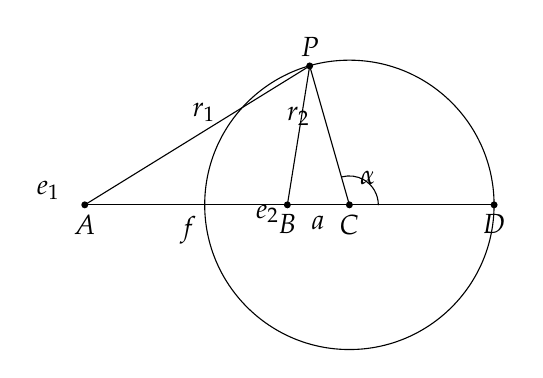
\begin{tikzpicture}[scale=1.05,line cap=round,line join=round]
  \coordinate (C) at (0,0);
  \coordinate (A) at (-3.2,0);
  \coordinate (B) at (-0.75,0);
  \coordinate (D) at (1.75,0);
  \coordinate (P) at (-0.48,1.68);
  \draw (C) circle (1.75);
  \draw (A)--(D);
  \draw (A)--(P);
  \draw (B)--(P);
  \draw (C)--(P);
  \foreach \pt in {A,B,C,D,P} \fill (\pt) circle (1.2pt);
  \node[below] at (A) {$A$};
  \node[below] at (B) {$B$};
  \node[below] at (C) {$C$};
  \node[below] at (D) {$D$};
  \node[above] at (P) {$P$};
  \node[left] at ($(A)+(-0.18,0.18)$) {$e_1$};
  \node[below left] at ($(B)+(0.02,0.12)$) {$e_2$};
  \node[below] at (-1.95,-0.02) {$f$};
  \node[below] at (-0.38,-0.02) {$a$};
  \node[above,sloped] at ($(A)!0.53!(P)$) {$r_1$};
  \node[above,sloped] at ($(B)!0.50!(P)$) {$r_2$};
  \draw (0.35,0) arc[start angle=0,end angle=105,radius=0.35];
  \node at (0.22,0.32) {$\alpha$};
\end{tikzpicture}

Fig. 7.
\end{center}

Let the charges of $A$ and $B$ be $e_1$ and $e_2$ respectively. Let $P$ be any point in space whose distances from $A$ and $B$ are $r_1$ and $r_2$ respectively. Then the value of the potential at $P$ will be

\begin{equation}\tag{1}
V=\frac{e_1}{r_1}+\frac{e_2}{r_2}.
\end{equation}

The equipotential surfaces due to this distribution of electricity are represented in Fig. I (at the end of this volume) when $e_1$ and $e_2$ are of the same sign, and in Fig. II when they are of opposite signs. We have now to consider that surface for which $V=0$, which is the only spherical surface in the system. When $e_1$ and $e_2$ are of the same sign, this surface is entirely at an infinite distance, but when they are of opposite signs there is a plane or spherical surface at a finite distance for which the potential is zero.

The equation of this surface is

\begin{equation}\tag{2}
\frac{e_1}{r_1}+\frac{e_2}{r_2}=0.
\end{equation}

Its centre is at a point $C$ in $AB$ produced, such that

\[
AC:BC::e_1^2:e_2^2,
\]

and the radius of the sphere is

\[
AB\frac{e_{1}e_{2}}{{e_{1}}^{2}-{e_{2}}^{2}}\cdot
\]

The two points $A$ and $B$ are inverse points with respect to this sphere, that is to say, they lie in the same radius, and the radius is a mean proportional between their distances from the centre.

Since this spherical surface is at potential zero, if we suppose it constructed of thin metal and connected with the earth, there will be no alteration of the potential at any point either outside or inside, but the electrical action everywhere will remain that due to the two electrified points $A$ and $B$.

If we now keep the metallic shell in connexion with the earth and remove the point $B$, the potential within the sphere will become everywhere zero, but outside it will remain the same as before. For the surface of the sphere still remains at the same potential, and no change has been made in the exterior electrification.

Hence, if an electrified point $A$ be placed outside a spherical conductor which is at potential zero, the electrical action at all points outside the sphere will be that due to the point $A$ together with another point $B$ within the sphere, which we may call the electrical image of $A$.

In the same way we may shew that if $B$ is a point placed inside the spherical shell, the electrical action within the sphere is that due to $B$, together with its image $A$.

157.] \emph{Definition of an Electrical Image.} An electrical image is an electrified point or system of points on one side of a surface which would produce on the other side of that surface the same electrical action which the actual electrification of that surface really does produce.

In Optics a point or system of points on one side of a mirror or lens which if it existed would emit the system of rays which actually exists on the other side of the mirror or lens, is called a virtual image.

Electrical images correspond to virtual images in optics in being related to the space on the other side of the surface. They do not correspond to them in actual position, or in the merely approximate character of optical foci.

There are no \emph{real} electrical images, that is, imaginary electrified points which would produce, in the region on the same side of the electrified surface, an effect equivalent to that of the electrified surface.

For if the potential in any region of space is equal to that due to a certain electrification in the same region it must be actually produced by that electrification. In fact, the electrification at any point may be found from the potential near that point by the application of Poisson's equation.

Let $a$ be the radius of the sphere.

Let $f$ be the distance of the electrified point $A$ from the centre $C$. Let $e$ be the charge of this point.

Then the image of the point is at $B$, on the same radius of the sphere at a distance $\frac{a^2}{f}$, and the charge of the image is $-e\frac{a}{f}$.

We have shewn that this image will produce the same effect on the opposite side of the surface as the actual electrification of the surface does. We shall next determine the surface-density of this electrification at any point $P$ of the spherical surface, and for this purpose we shall make use of the theorem of Coulomb,

Art. 80, that if $R$ is the resultant force at the surface of a conductor, and $\sigma$ the superficial density,

\[
R=4\pi\sigma,
\]

$R$ being measured away from the surface.

We may consider $R$ as the resultant of two forces, a repulsion $\frac{e}{AP^2}$ acting along $AP$, and an attraction $e\frac{a}{f}\frac{1}{PB^2}$ acting along $PB$.

Resolving these forces in the directions of AC and CP, we find that the components of the repulsion are

\[
\frac{ef}{AP^3}\quad\hbox{along }AC,\qquad
\frac{ea}{AP^3}\quad\hbox{along }CP.
\]

Those of the attraction are

\[
-e\frac{a}{f}\frac{1}{BP^3}BC\quad\hbox{along }AC,\qquad
-e\frac{a^2}{f}\frac{1}{BP^3}\quad\hbox{along }CP.
\]

Now $BP=\frac{a}{f}AP$, and $BC=\frac{a^2}{f}$, so that the components of

the attraction may be written

\[
-ef\frac{1}{AP^3}\quad\hbox{along }AC,\qquad
-e\frac{f^2}{a}\frac{1}{AP^3}\quad\hbox{along }CP.
\]

The components of the attraction and the repulsion in the direction of $AC$ are equal and opposite, and therefore the resultant force is entirely in the direction of the radius $CP$. This only confirms what we have already proved, that the sphere is an equipotential surface, and therefore a surface to which the resultant force is everywhere perpendicular.

The resultant force measured along $CP$, the normal to the surface in the direction towards the side on which $A$ is placed, is

\begin{equation}\tag{3}
R=-e\frac{f^2-a^2}{a}\frac{1}{AP^3}.
\end{equation}

If $A$ is taken inside the sphere $f$ is less than $a$, and we must measure $R$ inwards. For this case therefore

\begin{equation}\tag{4}
R=-e\frac{a^2-f^2}{a}\frac{1}{AP^3}.
\end{equation}

In all cases we may write

\begin{equation}\tag{5}
R = -e\frac{AD.Ad}{CP} \frac{1}{AP^3},
\end{equation}

where $AD$, $Ad$ are the segments of any line through $A$ cutting the sphere, and their product is to be taken positive in all cases.

158.] From this it follows, by Coulomb's theorem, Art. 80, that the surface-density at $P$ is

\begin{equation}\tag{6}
\sigma = -e \frac{AD \cdot Ad}{4\pi \cdot CP} \frac{1}{AP^3}.
\end{equation}

The density of the electricity at any point of the sphere varies inversely as the cube of its distance from the point $A$.

The effect of this superficial distribution, together with that of the point $A$, is to produce on the same side of the surface as the point $A$ a potential equivalent to that due to $e$ at $A$, and its image $-e\frac{a}{f}$ at $B$, and on the other side of the surface the potential is everywhere zero. Hence the effect of the superficial distribution by itself is to produce a potential on the side of $A$ equivalent to that due to the image $-e\frac{a}{f}$ at $B$, and on the opposite side a potential equal and opposite to that of $e$ at $A$.

The whole charge on the surface of the sphere is evidently $-e\frac{a}{f}$ since it is equivalent to the image at $B$.

We have therefore arrived at the following theorems on the action of a distribution of electricity on a spherical surface, the surface-density being inversely as the cube of the distance from a point $A$ either without or within the sphere.

Let the density be given by the equation

\begin{equation}\tag{7}
\sigma=\frac{C}{AP^3},
\end{equation}

where $C$ is some constant quantity, then by equation (6)

\begin{equation}\tag{8}
C = -e \frac{AD \cdot Ad}{4\pi a} \,.
\end{equation}

The action of this superficial distribution on any point separated from $A$ by the surface is equal to that of a quantity of electricity

\[
-e,\quad\hbox{or}\quad
\frac{4\pi aC}{AD\cdot Ad}
\]

concentrated at $A$.

Its action on any point on the same side of the surface with $A$ is equal to that of a quantity of electricity

\[
\frac{4\pi Ca^2}{f\,AD\cdot Ad}
\]

concentrated at $B$ the image of $A$.

The whole quantity of electricity on the sphere is equal to the first of these quantities if $A$ is within the sphere, and to the second if $A$ is without the sphere.

These propositions were established by Sir W. Thomson in his original geometrical investigations with reference to the distribution of electricity on spherical conductors, to which the student ought to refer.

159.] If a system in which the distribution of electricity is known is placed in the neighbourhood of a conducting sphere of radius $a$, which is maintained at potential zero by connexion with the earth, then the electrifications due to the several parts of the system will be superposed.

Let $A_1$, $A_2$, \&c. be the electrified points of the system, $f_1$, $f_2$, \&c. their distances from the centre of the sphere, $e_1$, $e_2$, \&c. their charges, then the images $B_1$, $B_2$, \&c. of these points will be in the same radii as the points themselves, and at distances $\frac{a^2}{f_1}$, $\frac{a^2}{f_2}$, \&c. from the centre of the sphere, and their charges will be

\[
-e_1\frac{a}{f_1},\quad -e_2\frac{a}{f_2},\quad\hbox{\&c.}
\]

The potential on the outside of the sphere due to the superficial electrification will be the same as that which would be produced by the system of images $B_1$, $B_2$, \&c. This system is therefore called the electrical image of the system $A_1$, $A_2$, \&c.

If the sphere instead of being at potential zero is at potential $V$, we must superpose a distribution of electricity on its outer surface having the uniform surface-density

\[
\sigma=\frac{V}{4\pi a^2}.
\]

The effect of this at all points outside the sphere will be equal to that of a quantity $Va$ of electricity placed at its centre, and at all points inside the sphere the potential will be simply increased by $V$.

The whole charge on the sphere due to an external system of influencing points $A_1$, $A_2$, \&c. is

\begin{equation}\tag{9}
E=Va-e_1\frac{a}{f_1}-e_2\frac{a}{f_2}-\hbox{\&c.},
\end{equation}

from which either the charge $E$ or the potential $V$ may be calculated when the other is given.

When the electrified system is within the spherical surface the induced charge on the surface is equal and of opposite sign to the inducing charge, as we have before proved it to be for every closed surface, with respect to points within it.

160.] The energy due to the mutual action between an electrified point $e$, at a distance $f$ from the centre of the sphere greater than $a$ the radius, and the electrification of the spherical surface due to the influence of the electrified point and the charge of the sphere, is

\begin{equation}\tag{10}
M=e\left(\frac{Va}{f}-\frac{ea}{f^2-a^2}\right)
=\frac{e}{f}\left(E-\frac{e^2a^3}{f(f^2-a^2)}\right),
\end{equation}

where $V$ is the potential, and $E$ the charge of the sphere.

The repulsion between the electrified point and the sphere is therefore, by Art. 92,

\begin{equation}\tag{11}
F=ea\left(\frac{V}{f^2}-\frac{ef}{(f^2-a^2)^2}\right)
=\frac{e}{f^2}\left(E-e\frac{a^3(2f^2-a^2)}{f(f^2-a^2)^2}\right).
\end{equation}

Hence the force between the point and the sphere is always an attraction in the following cases--

(1) When the sphere is uninsulated.

(2) When the sphere has no charge.

(3) When the electrified point is very near the surface.

In order that the force may be repulsive, the potential of the sphere must be positive and greater than $e\frac{f^3}{(f^2-a^2)^2}$, and the charge of the sphere must be of the same sign as $e$ and greater than $e\frac{a^3(2f^2-a^2)}{f(f^2-a^2)^2}$.

At the point of equilibrium the equilibrium is unstable, the force

being an attraction when the bodies are nearer and a repulsion when they are farther off.

When the electrified point is within the spherical surface the force on the electrified point is always away from the centre of the sphere, and is equal to

\[
\frac{e^2af}{(a^2-f^2)^2}.
\]

The surface-density at the point of the sphere nearest to the electrified point where it lies outside the sphere is

\begin{equation}\tag{12}
\begin{split}
\sigma_1&=\frac{1}{4\pi a^2}
\left\{Va-e\frac{a(f+a)}{(f-a)^2}\right\}\\
&=\frac{1}{4\pi a^2}
\left\{E-e\frac{a^2(3f-a)}{f(f-a)^2}\right\}.
\end{split}
\end{equation}

The surface-density at the point of the sphere farthest from the electrified point is

\begin{equation}\tag{13}
\begin{split}
\sigma_2&=\frac{1}{4\pi a^2}
\left\{Va-e\frac{a(f-a)}{(f+a)^2}\right\}\\
&=\frac{1}{4\pi a^2}
\left\{E+e\frac{a^2(3f+a)}{f(f+a)^2}\right\}.
\end{split}
\end{equation}

When $E$, the charge of the sphere, lies between

\[
e\frac{a^2(3f-a)}{f(f-a)^2}
\]
and $-e\frac{a^2(3f+a)}{f(f+a)^2}$

the electrification will be negative next the electrified point and positive on the opposite side. There will be a circular line of division between the positively and the negatively electrified parts of the surface, and this line will be a line of equilibrium.

If
\begin{equation}\tag{14}
E=ea\left(\frac{1}{\sqrt{f^2-a^2}}-\frac{1}{f}\right),
\end{equation}

the equipotential surface which cuts the sphere in the line of equilibrium is a sphere whose centre is the electrified point and whose radius is  $\sqrt{f^2-a^2}$ .

The lines of force and equipotential surfaces belonging to a case of this kind are given in Figure IV at the end of this volume.

{\centering\itshape Images in an Infinite Plane Conducting Surface.\par}

161.] If the two electrified points $A$ and $B$ in Art. 156 are electrified with equal charges of electricity of opposite signs, the surface of zero potential will be the plane, every point of which is equidistant from $A$ and $B$.

% batch_0238
\setcounter{footnote}{0}
Hence, if A be an electrified point whose charge is $e$, and $AD$
a perpendicular on the plane, produce $AD$ to $B$ so that $DB=AB$,
and place at $B$ a charge equal to $-e$, then this charge at $B$
will be the image of $A$, and will produce at all points on the same
side of the plane as $A$, an effect equal to that of the actual
electrification of the plane. For the potential on the side of $A$
due to $A$ and $B$ fulfils the conditions that $\nabla^2 V=0$
everywhere except at $A$, and that $V=0$ at the plane, and there is
only one form of $V$ which can fulfil these conditions.

\begin{center}
\begin{tikzpicture}[scale=0.9, line cap=round, line join=round]
  \coordinate (D) at (0,0);
  \coordinate (A) at (-2.3,0);
  \coordinate (B) at (2.3,0);
  \coordinate (P) at (0,1.45);
  \draw[gray!75] (0,-0.85) -- (0,2.25);
  \draw (A) -- (B);
  \draw (A) -- (P) -- (B);
  \fill (A) circle (1.2pt) node[below left] {$A$};
  \fill (B) circle (1.2pt) node[below right] {$B$};
  \fill (D) circle (1.2pt) node[below] {$D$};
  \fill (P) circle (1.2pt) node[above left] {$P$};
  \node[below] at (-1.75,0) {$e$};
  \node[below] at (1.75,0) {$-e$};
\end{tikzpicture}

Fig. 8.
\end{center}

To determine the resultant force at the point P of the plane, we observe that it is compounded of two forces each equal to  $\frac{e}{AP^2}$ , one acting along AP and the other along PB. Hence the resultant of these forces is in a direction parallel to AB and equal to

\[
\frac{e}{AP^2}\cdot\frac{AB}{AP}.
\]

Hence R, the resultant force measured from the surface towards the space in which A lies, is

\begin{equation}\tag{15}
R = -\frac{2eAD}{AP^3},
\end{equation}

and the density at the point P is

\begin{equation}\tag{16}
\sigma = -\frac{eAD}{2\pi AP^3}.
\end{equation}

\begin{center}
\textit{On Electrical Inversion.}
\end{center}

162.] The method of electrical images leads directly to a method of transformation by which we may derive from any electrical problem of which we know the solution any number of other problems with their solutions.

We have seen that the image of a point at a distance $r$ from the
centre of a sphere of radius $R$ is in the same radius and at a
distance $r'$ such that $rr'=R^2$. Hence the image of a system of
points, lines, or surfaces is obtained from the original system by the
method known in pure geometry as the method of inversion, and described
by Chasles, Salmon, and other mathematicians.

If $A$ and $B$ are two points, $A'$ and $B'$ their images, $O$ being
the centre of inversion, and $R$ the radius of the sphere of inversion,

\begin{center}
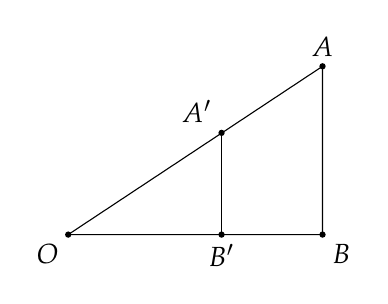
\begin{tikzpicture}[scale=0.95, line cap=round, line join=round]
  \coordinate (O) at (0,0);
  \coordinate (B) at (3.4,0);
  \coordinate (A) at (3.4,2.25);
  \coordinate (Bp) at (2.05,0);
  \coordinate (Ap) at (2.05,1.36);
  \draw (O) -- (B) -- (A) -- cycle;
  \draw (Bp) -- (Ap);
  \fill (O) circle (1.2pt) node[below left] {$O$};
  \fill (B) circle (1.2pt) node[below right] {$B$};
  \fill (A) circle (1.2pt) node[above] {$A$};
  \fill (Bp) circle (1.2pt) node[below] {$B'$};
  \fill (Ap) circle (1.2pt) node[above left] {$A'$};
\end{tikzpicture}

Fig. 9.
\end{center}

\[
OA.OA' = R^2 = OB.OB'.
\]

Hence the triangles $OAB$, $OB'A'$ are similar, and
$AB:A'B'::OA:OB'::OA.OB:R^2$.

Hence

If a quantity of electricity $e$ be placed at $A$,

its potential at $B$ will be

\[
V = \frac{e}{AB}.
\]

If $e'$ be placed at $A'$ its potential at $B'$ will be

\[
V' = \frac{e'}{A'B'}.
\]

In the theory of electrical images

\[
e : e' :: OA : R :: R : OA'.
\]
\begin{equation}\tag{17}
V:V'::R:OB,
\end{equation}

or the potential at $B$ due to the electricity at $A$ is to the
potential at the image of $B$ due to the electrical image of $A$ as
$R$ is to $OB$.

Since this ratio depends only on $OB$ and not on $OA$, the potential
at $B$ due to any system of electrified bodies is to that at $B'$ due
to the image of the system as $R$ is to $OB$.

If $r$ be the distance of any point $A$ from the centre, and $r'$ that
of its image $A'$, and if $e$ be the electrification of $A$, and $e'$
that of $A'$, also if $L$, $S$, $K$ be linear, superficial, and solid
elements at $A$, and $L'$, $S'$, $K'$ their images at $A'$, and
$\lambda$, $\sigma$, $\rho$, $\lambda'$, $\sigma'$, $\rho'$ the
corresponding line-surface and volume-densities of electricity at the
two points, $V$ the potential at $A$ due to the original system, and
$V'$ the potential at $A'$ due to the inverse system, then

\begin{equation}\tag{18}
\begin{aligned}
\frac{r'}{r}=\frac{L'}{L}
  &=\frac{R^2}{r^2}=\frac{r'^2}{R^2},&
\frac{S'}{S}
  &=\frac{R^4}{r^4}=\frac{r'^4}{R^4},&
\frac{K'}{K}
  &=\frac{R^6}{r^6}=\frac{r'^6}{R^6};\\
\frac{e'}{e}
  &=\frac{R}{r}=\frac{r'}{R},&
\frac{\lambda'}{\lambda}
  &=\frac{r}{R}=\frac{R}{r'},\\
\frac{\sigma'}{\sigma}
  &=\frac{r^3}{R^3}=\frac{R^3}{r'^3},&
\frac{\rho'}{\rho}
  &=\frac{r^5}{R^5}=\frac{R^5}{r'^5},\\
\frac{V'}{V}
  &=\frac{r}{R}=\frac{R}{r'}.
\end{aligned}
\end{equation}

If in the original system a certain surface is that of a conductor,\footnote{See Thomson and Tait's \textit{Natural Philosophy}, \S 515.}

and has therefore a constant potential $P$, then in the transformed
system the image of the surface will have a potential $P\frac{R}{r'}$.
But by placing at $O$, the centre of inversion, a quantity of
electricity equal to $-PR$, the potential of the transformed surface is
reduced to zero.

Hence, if we know the distribution of electricity on a conductor when
insulated in open space and charged to the potential $P$, we can find
by inversion the distribution on a conductor whose form is the image of
the first under the influence of an electrified point with a charge
$-PR$ placed at the centre of inversion, the conductor being in
connexion with the earth.

163.] The following geometrical theorems are useful in studying cases of inversion.

Every sphere becomes, when inverted, another sphere, unless it passes through the centre of inversion, in which case it becomes a plane.

If the distances of the centres of the spheres from the centre of
inversion are $a$ and $a'$, and if their radii are $\alpha$ and
$\alpha'$, and if we define the \textit{power} of the sphere with
respect to the centre of inversion to be the product of the segments
cut off by the sphere from a line through the centre of inversion, then
the power of the first sphere is $a^2-\alpha^2$, and that of the second
is $a'^2-\alpha'^2$. We have in this case

\begin{equation}\tag{19}
\frac{a'}{a}
=\frac{\alpha'}{\alpha}
=\frac{R^2}{a^2-\alpha^2}
=\frac{a'^2-\alpha'^2}{R^2},
\end{equation}

or the ratio of the distances of the centres of the first and second spheres is equal to the ratio of their radii, and to the ratio of the power of the sphere of inversion to the power of the first sphere, or of the power of the second sphere to the power of the sphere of inversion.

The centre of either sphere corresponds to the inverse point of the
other with respect to the centre of inversion.

In the case in which the inverse surfaces are a plane and a sphere,
the perpendicular from the centre of inversion on the plane is to the
radius of inversion as this radius is to the diameter of the sphere,
and the sphere has its centre on this perpendicular and passes through
the centre of inversion.

Every circle is inverted into another circle unless it passes through
the centre of inversion, in which case it becomes a straight line. The
angle between two surfaces, or two lines at their intersection, is not
changed by inversion.

Every circle which passes through a point, and the image of that point
with respect to a sphere, cuts the sphere at right angles.

Hence, any circle which passes through a point and cuts the sphere at
right angles passes through the image of the point.

164.] We may apply the method of inversion to deduce the distribution
of electricity on an uninsulated sphere under the influence of an
electrified point from the uniform distribution on an insulated sphere
not influenced by any other body.

If the electrified point be at $A$, take it for the centre of
inversion, and if $A$ is at a distance $f$ from the centre of the
sphere whose radius is $a$, the inverted figure will be a sphere whose
radius is $a'$ and whose centre is distant $f'$, where

\begin{equation}\tag{20}
\frac{a'}{a}=\frac{f'}{f}=\frac{R^2}{f^2-a^2}.
\end{equation}

The centre of either of these spheres corresponds to the inverse point
of the other with respect to $A$, or if $C$ is the centre and $B$ the
inverse point of the first sphere, $C'$ will be the inverse point, and
$B'$ the centre of the second.

Now let a quantity $e'$ of electricity be communicated to the second
sphere, and let it be uninfluenced by external forces. It will become
uniformly distributed over the sphere with a surface-density

\begin{equation}\tag{21}
\sigma' = \frac{e'}{4\pi a'^2}.
\end{equation}

Its action at any point outside the sphere will be the same as that of
a charge $e'$ placed at $B'$ the centre of the sphere.

At the spherical surface and within it the potential is

\begin{equation}\tag{22}
P' = \frac{e'}{a'},
\end{equation}

a constant quantity.

Now let us invert this system. The centre $B'$ becomes in the inverted
system the inverse point $B$, and the charge $e'$ at $B'$ becomes
$e'\frac{AB}{R}$ at $B$, and at any point separated from $B$ by the
surface the potential is that due to this charge at $B$.

The potential at any point $P$ on the spherical surface, or on the same
side as $B$, is in the inverted system

\[
\frac{e'}{a'}\frac{R}{AP}.
\]

If we now superpose on this system a charge $e$ at $A$, where

\begin{equation}\tag{23}
e = -\frac{e'}{a'}R,
\end{equation}

the potential on the spherical surface, and at all points on the same
side as $B$, will be reduced to zero. At all points on the same side
as $A$ the potential will be that due to a charge $e$ at $A$, and a
charge $e'\frac{R}{f'}$ at $B$.

\begin{equation}\tag{24}
e'\frac{R}{f'}=-e\frac{a'}{f'}=-e\frac{a}{f},
\end{equation}

as we found before for the charge of the image at $B$.

To find the density at any point of the first sphere we have

\begin{equation}\tag{25}
\sigma=\sigma'\frac{R^3}{AP^3}.
\end{equation}

Substituting for the value of $\sigma'$ in terms of the quantities
belonging to the first sphere, we find the same value as in Art. 158,

\begin{equation}\tag{26}
\sigma=-\frac{e(f^2-a^2)}{4\pi aAP^3}.
\end{equation}

\begin{center}
\textit{On Finite Systems of Successive Images.}
\end{center}

165.] If two conducting planes intersect at an angle which is a
submultiple of two right angles, there will be a finite system of
images which will completely determine the electrification.

For let $AOB$ be a section of the two conducting planes perpendicular
to their line of intersection, and let the angle of intersection
$AOB=\frac{\pi}{n}$, let $P$ be an electrified point, and let $PO=r$,
and $POB=\theta$. Then, if we draw a circle with centre $O$ and radius
$OP$, and find points which are the successive images of $P$ in the two
planes beginning with $OB$, we shall find $Q_1$ for the image of $P$ in
$OB$, $P_2$ for the image of $Q_1$ in $OA$, $Q_3$ for that of $P_2$ in
$OB$, $P_3$ for that of $Q_3$ in $OA$, and $Q_2$ for that of $P_3$ in
$OB$.

\begin{center}
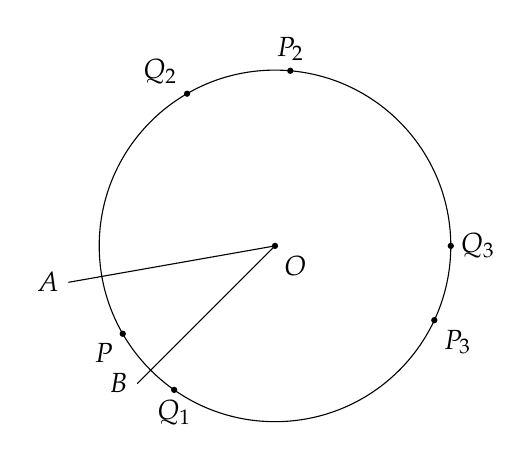
\begin{tikzpicture}[scale=0.95, line cap=round, line join=round]
  \coordinate (O) at (0,0);
  \def\r{2.35}
  \draw (O) circle (\r);
  \draw (O) -- ++(190:2.8) node[left] {$A$};
  \draw (O) -- ++(225:2.6) node[left] {$B$};
  \foreach \ang/\lab/\pos in {210/P/below left,235/Q_1/below,85/P_2/above,120/Q_2/above left,0/Q_3/right,335/P_3/below right} {
    \coordinate (X) at (\ang:\r);
    \fill (X) circle (1.2pt) node[\pos] {$\lab$};
  }
  \fill (O) circle (1.2pt) node[below right] {$O$};
\end{tikzpicture}

Fig. 10.
\end{center}

If we had begun with the image of $P$ in $AO$ we should have found the
same points in the reverse order $Q_2$, $P_3$, $Q_3$, $P_2$, $Q_1$,
provided $AOB$ is a submultiple of two right angles.

For the alternate images $P_1$, $P_2$, $P_3$ are ranged round the
circle at angular intervals equal to $2AOB$, and the intermediate
images $Q_1$, $Q_2$, $Q_3$ are at intervals of the same magnitude.
Hence, if $2AOB$ is a submultiple of $2\pi$, there will be a finite
number of images, and none of these will fall within the angle $AOB$.
If, however, $AOB$ is not a submultiple of $\pi$, it will be impossible
to represent the actual electrification as the result of a finite
series of electrified points.

If $AOB=\frac{\pi}{n}$, there will be $n$ negative images $Q_1$,
$Q_2$, \&c., each equal and of opposite sign to $P$, and $n-1$
positive images $P_2$, $P_3$, \&c., each equal to $P$, and of the same
sign.

The angle between successive images of the same sign is  $\frac{2\pi}{n}$ .

If we consider either of the conducting planes as a plane of symmetry,
we shall find the positive and negative images placed symmetrically
with regard to that plane, so that for every positive image there is a
negative image in the same normal, and at an equal distance on the
opposite side of the plane.

If we now invert this system with respect to any point, the two planes
become two spheres, or a sphere and a plane intersecting at an angle
$\frac{\pi}{n}$, the influencing point $P$ being within this angle.

The successive images lie on the circle which passes through $P$ and
intersects both spheres at right angles.

To find the position of the images we may either make use of the
principle that a point and its image are in the same radius of the
sphere, and draw successive chords of the circle beginning at $P$ and
passing through the centres of the two spheres alternately.

To find the charge which must be attributed to each image, take any
point in the circle of intersection, then the charge of each image is
proportional to its distance from this point, and its sign is positive
or negative according as it belongs to the first or the second system.

166.] We have thus found the distribution of the images when any space
bounded by a conductor consisting of two spherical surfaces meeting at
an angle $\frac{\pi}{n}$, and kept at potential zero, is influenced by
an electrified point.

We may by inversion deduce the case of a conductor consisting

of two spherical segments meeting at a re-entering angle
$\frac{\pi}{n}$, charged to potential unity and placed in free space.

For this purpose we invert the system with respect to $P$. The circle
on which the images formerly lay now becomes a straight line through
the centres of the spheres.

If the figure (11) represents a section through the line of centres
$AB$, and if $D$, $D'$ are the points where the circle of intersection
cuts the plane of the paper, then, to find the successive images, draw
$DA$ a radius of the first circle, and draw $DC$, $DB$, \&c., making
angles $\frac{\pi}{n}$, $\frac{2\pi}{n}$, \&c. with $DA$.

\begin{center}
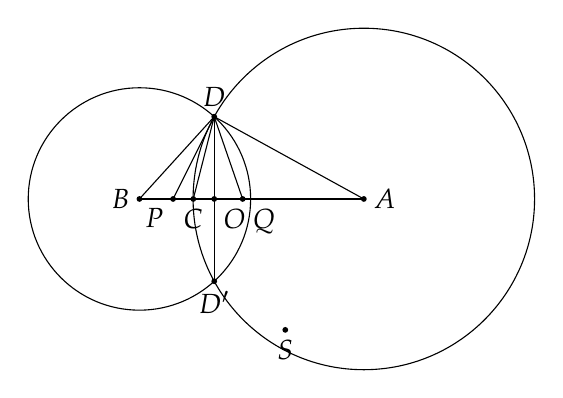
\begin{tikzpicture}[scale=0.95, line cap=round, line join=round]
  \coordinate (D) at (0,1.1);
  \coordinate (Dp) at (0,-1.1);
  \coordinate (O) at (0,0);
  \coordinate (A) at (2.0,0);
  \coordinate (B) at (-1.0,0);
  \coordinate (C) at (-0.28,0);
  \coordinate (P) at (-0.55,0);
  \coordinate (Q) at (0.38,0);
  \coordinate (S) at (0.95,-1.75);
  \draw (A) circle ({sqrt(5.21)});
  \draw (B) circle ({sqrt(2.21)});
  \draw (B) -- (A);
  \draw (D) -- (A);
  \draw (D) -- (B);
  \draw (D) -- (C);
  \draw (D) -- (P);
  \draw (D) -- (Q);
  \draw (D) -- (Dp);
  \foreach \pt in {A,B,C,P,Q,O,D,Dp,S} {
    \fill (\pt) circle (1.1pt);
  }
  \node[right] at (A) {$A$};
  \node[left] at (B) {$B$};
  \node[below left] at (P) {$P$};
  \node[below] at (C) {$C$};
  \node[below right] at (Q) {$Q$};
  \node[above] at (D) {$D$};
  \node[below] at (Dp) {$D'$};
  \node[below right] at (O) {$O$};
  \node[below] at (S) {$S$};
\end{tikzpicture}

Fig. 11.
\end{center}

The points $C$, $B$, \&c. at which they cut the line of centres will be
the positions of the positive images, and the charge of each will be
represented by its distances from $D$. The last of these images will
be at the centre of the second circle.

To find the negative images draw $DP$, $DQ$, \&c., making angles
$\frac{\pi}{n}$, $\frac{2\pi}{n}$, \&c. with the line of centres. The
intersections of these lines with the line of centres will give the
positions of the negative images, and the charge of each will be
represented by its distance from $D$.

The surface-density at any point of either sphere is the sum of the
surface-densities due to the system of images. For instance, the
surface-density at any point $S$ of the sphere whose centre is $A$, is

\[
\sigma = \frac{1}{4\pi DA}\left\{
1+(AD^2-AB^2)\frac{DB}{BS^3}
 +(AD^2-AC^2)\frac{DC}{CS^3}+\&c.\right\},
\]

where $A$, $B$, $C$, \&c. are the positive series of images.

When $S$ is on the circle of intersection the density is zero.

To find the total charge on each of the spherical segments, we may find
the surface-integral of the induction through that segment due to each
of the images.

The total charge on the segment whose centre is $A$ due to the image
at $A$ whose charge is $DA$ is

\[
DA\frac{DA+OA}{2DA}=\frac{1}{2}(DA+OA),
\]

where $O$ is the centre of the circle of intersection.

In the same way the charge on the same segment due to the image at
$B$ is $\frac{1}{2}(DB+OB)$, and so on, lines such as $OB$ measured
from $O$ to the left being reckoned negative.

Hence the total charge on the segment whose centre is $A$ is

\[
\frac{1}{2}(DA+DB+DC+\&c.)+\frac{1}{2}(OA+OB+OC+\&c.),
\]

\[
-\frac{1}{2}(DP+DQ+\&c.)-\frac{1}{2}(OP+OQ+\&c.).
\]

167.] The method of electrical images may be applied to any space
bounded by plane or spherical surfaces all of which cut one another in
angles which are submultiples of two right angles.

In order that such a system of spherical surfaces may exist, every
solid angle of the figure must be trihedral, and two of its angles must
be right angles, and the third either a right angle or a submultiple of
two right angles.

Hence the cases in which the number of images is finite are

\begin{enumerate}
\item A single spherical surface or a plane.
\item Two planes, a sphere and a plane, or two spheres intersecting at
an angle $\frac{\pi}{n}$.
\item These two surfaces with a third, which may be either plane or
spherical, cutting both orthogonally.
\item These three surfaces with a fourth cutting the first two
orthogonally and the third at an angle $\frac{\pi}{n'}$. Of these four
surfaces one at least must be spherical.
\end{enumerate}

We have already examined the first and second cases. In the first case
we have a single image. In the second case we have $2n-1$ images
arranged in two series in a circle which passes through the influencing
point and is orthogonal to both surfaces. In the third case we have,
besides these images, their images with respect to the third surface,
that is, $4n-1$ images in all besides the influencing point.

In the fourth case we first draw through the influencing point a circle
orthogonal to the first two surfaces, and determine on it the positions
and magnitudes of the $n$ negative images and the $n-1$ positive
images. Then through each of these $2n$ points, including the
influencing point, we draw a circle orthogonal to the third and fourth
surfaces, and determine on it two series of

images, $n'$ in each series. We shall obtain in this way, besides the
influencing point, $2nn'-1$ positive and $2nn'$ negative images. These
$4nn'$ points are the intersections of $n$ circles with $n'$ other
circles, and these circles belong to the two systems of lines of
curvature of a cyclide.

If each of these points is charged with the proper quantity of
electricity, the surface whose potential is zero will consist of
$n+n'$ spheres, forming two series of which the successive spheres of
the first set intersect at angles $\frac{\pi}{n}$, and those of the
second set at angles

$\frac{\pi}{n'}$, while every sphere of the first set is orthogonal to
every sphere of the second set.

\begin{center}
\textit{Case of Two Spheres cutting Orthogonally.} See Fig. IV at the
end of this volume.
\end{center}

168.] Let $A$ and $B$, Fig. 12, be the centres of two spheres cutting

each other orthogonally in $D$ and $D'$, and let the straight line
$DD'$ cut the line of centres in $C$. Then $C$ is the image of $A$ with
respect to the sphere $B$, and also the image of $B$ with respect to
the sphere whose centre is $A$. If $AD=a$, $BD=\beta$, then
$AB=\sqrt{a^2+\beta^2}$, and if we place at $A$, $B$, $C$ quantities

\begin{center}
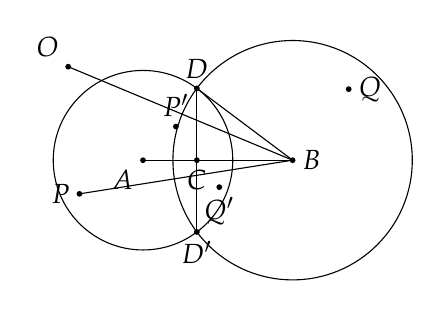
\begin{tikzpicture}[scale=0.95, line cap=round, line join=round]
  \coordinate (A) at (-1,0);
  \coordinate (B) at (1,0);
  \coordinate (C) at (-0.28,0);
  \coordinate (D) at (-0.28,0.96);
  \coordinate (Dp) at (-0.28,-0.96);
  \coordinate (O) at (-2.0,1.25);
  \coordinate (P) at (-1.85,-0.45);
  \coordinate (Pp) at (-0.56,0.45);
  \coordinate (Q) at (1.75,0.95);
  \coordinate (Qp) at (0.02,-0.36);
  \draw (A) circle (1.2);
  \draw (B) circle (1.6);
  \draw (A) -- (B);
  \draw (D) -- (Dp);
  \draw (O) -- (B);
  \draw (P) -- (B);
  \draw (D) -- (B);
  \foreach \pt/\lab/\pos in {O/O/above left,A/A/below left,B/B/right,C/C/below,D/D/above,Dp/D'/below,P/P/left,Pp/P'/above,Q/Q/right,Qp/Q'/below} {
    \fill (\pt) circle (1.1pt) node[\pos] {$\lab$};
  }
\end{tikzpicture}

Fig. 12.
\end{center}

of electricity equal to $a$, $\beta$, and
$-\frac{a\beta}{\sqrt{a^2+\beta^2}}$ respectively, then both spheres
will be equipotential surfaces whose potential is unity.

We may therefore determine from this system the distribution of electricity in the following cases:

(1) On the conductor $PDQD'$ formed of the larger segments of both
spheres. Its potential is 1, and its charge is

\[
a+\beta-\frac{a\beta}{\sqrt{a^2+\beta^2}}=AD+BD-CD.
\]

This quantity therefore measures the capacity of such a figure when free from the inductive action of other bodies.

The density at any point $P$ of the sphere whose centre is $A$, and
the density at any point $Q$ of the sphere whose centre is $B$, are
respectively

\[
\frac{1}{4\pi a}\left(1-\left(\frac{\beta}{BP}\right)^3\right)
\quad\hbox{and}\quad
\frac{1}{4\pi\beta}\left(1-\left(\frac{a}{AQ}\right)^3\right).
\]

At the points of intersection, $D$, $D'$, the density is zero.

If one of the spheres is very much larger than the other, the density
at the vertex of the smaller sphere is ultimately three times that at
the vertex of the larger sphere.

(2) The lens $P'DQ'D'$ formed by the two smaller segments of the
spheres, charged with a quantity of electricity
$=-\frac{a\beta}{\sqrt{a^2+\beta^2}}$, and acted on by points $A$ and
$B$, charged with quantities $a$ and $\beta$, is also at potential
unity, and the density at any point is expressed by the same formulae.

(3) The meniscus $DPD'Q'$ formed by the difference of the segments
charged with a quantity $a$, and acted on by points $B$ and $C$,
charged respectively with quantities $\beta$ and
$\frac{-a\beta}{\sqrt{a^2+\beta^2}}$, is also in equilibrium at
potential unity.

(4) The other meniscus $QDP'D'$ under the action of $A$ and $C$.

We may also deduce the distribution of electricity on the following internal surfaces.

The hollow lens $P'DQ'D$ under the influence of the internal
electrified point $C$ at the centre of the circle $DD'$.

The hollow meniscus under the influence of a point at the centre of the concave surface.

The hollow formed of the two larger segments of both spheres under the
influence of the three points $A$, $B$, $C$.

But, instead of working out the solutions of these cases, we shall
apply the principle of electrical images to determine the density of
the electricity induced at the point $P$ of the external surface of the
conductor $PDQD'$ by the action of a point at $O$ charged with unit of
electricity.

Let 
\[
\begin{gathered}
OA=a,\quad OB=b,\quad OP=r,\quad BP=p,\\
AD=\alpha,\quad BD=\beta,\quad AB=\sqrt{\alpha^2+\beta^2}.
\end{gathered}
\]

Invert the system with respect to a sphere of radius unity and centre
$O$.

The two spheres will remain spheres, cutting each other orthogonally,
and having their centres in the same radii with $A$ and $B$. If we
indicate by accented letters the quantities corresponding to the
inverted system,

\[
\begin{aligned}
a' &= \frac{a}{a^2-\alpha^2}, \quad
b' = \frac{b}{b^2-\beta^2}, \quad
\alpha' = \frac{\alpha}{a^2-\alpha^2}, \quad
\beta' = \frac{\beta}{b^2-\beta^2}, \\
r' &= \frac{1}{r}, \quad
p'^2 = \frac{\beta^2 r^2+(b^2-\beta^2)(p^2-\beta^2)}
{r^2(b^2-\beta^2)^2}.
\end{aligned}
\]

% batch_0248
\setcounter{footnote}{0}
If, in the inverted system, the potential of the surface is unity, then
the density at the point $P'$ is

\[
\sigma'=\frac{1}{4\pi\alpha'}
\left(1-\left(\frac{\beta'}{p'}\right)^3\right).
\]

If, in the original system, the density at $P$ is $\sigma$, then

\[
\frac{\sigma}{\sigma'} = \frac{1}{r^3},
\]

and the potential is $\frac{1}{r}$. By placing at $O$ a negative
charge of electricity equal to unity, the potential will become zero
over the surface, and the density at $P$ will be

\[
\sigma=\frac{1}{4\pi}\frac{a^2-\alpha^2}{\alpha r^3}
\left(1-\frac{\beta^3r^3}
{\left(\beta^2r^2+(b^2-\beta^2)(p^2-\beta^2)\right)^{3/2}}\right).
\]

This gives the distribution of electricity on one of the spherical
surfaces due to a charge placed at $O$. The distribution on the other
spherical surface may be found by exchanging $a$ and $b$, $\alpha$ and
$\beta$, and putting $q$ or $AQ$ instead of $p$.

To find the total charge induced on the conductor by the electrified
point at $O$, let us examine the inverted system.

In the inverted system we have a charge $\alpha'$ at $A'$, and
$\beta'$ at $B'$, and a negative charge
$\frac{\alpha'\beta'}{\sqrt{\alpha'^2+\beta'^2}}$ at a point $C'$ in
the line $A'B'$,

such that

\[
A'C':C'B'::\alpha'^2:\beta'^2.
\]

If $OA'=a'$, $OB'=b'$, $OC'=c'$, we find

\[
c'^{2} =
\frac{a'^{2}\beta'^{2}+b'^{2}\alpha'^{2}-\alpha'^{2}\beta'^{2}}
{\alpha'^{2}+\beta'^{2}}.
\]

Inverting this system the charges become

\[
\frac{\alpha'}{a'}=\frac{\alpha}{a}, \quad
\frac{\beta'}{b'}=\frac{\beta}{b};
\]

and

\[
-\frac{\alpha'\beta'}{\sqrt{\alpha'^2+\beta'^2}}\frac{1}{c'}
=-\frac{\alpha\beta}
{\sqrt{a^2\beta^2+b^2\alpha^2-\alpha^2\beta^2}}.
\]

Hence the whole charge on the conductor due to a unit of negative
electricity at $O$ is

\[
\frac{\alpha}{a}+\frac{\beta}{b}
-\frac{\alpha\beta}
{\sqrt{a^2\beta^2+b^2\alpha^2-\alpha^2\beta^2}}.
\]

\begin{center}
\textit{Distribution of Electricity on Three Spherical Surfaces which
Intersect at Right Angles.}
\end{center}

169.] Let the radii of the spheres be $\alpha$, $\beta$, $\gamma$,
then

\[
BC=\sqrt{\beta^2+\gamma^2},\quad
CA=\sqrt{\gamma^2+\alpha^2},\quad
AB=\sqrt{\alpha^2+\beta^2}.
\]

\begin{center}
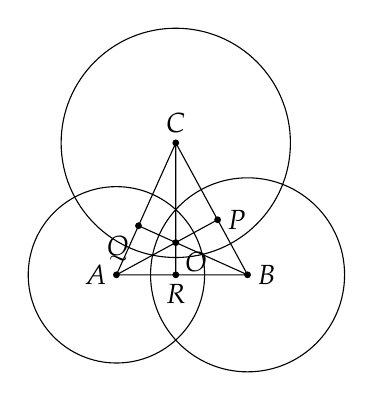
\begin{tikzpicture}[scale=1.12, line cap=round, line join=round]
  \def\al{1.00}
  \def\be{1.10}
  \def\ga{1.30}
  \coordinate (A) at (0,0);
  \coordinate (B) at (1.487,0);
  \coordinate (C) at (0.673,1.496);
  \coordinate (P) at ($(B)!(A)!(C)$);
  \coordinate (Q) at ($(A)!(B)!(C)$);
  \coordinate (R) at ($(A)!(C)!(B)$);
  \coordinate (O) at (0.673,0.365);
  \draw (A) circle (\al);
  \draw (B) circle (\be);
  \draw (C) circle (\ga);
  \draw (A) -- (B) -- (C) -- cycle;
  \draw (A) -- (P);
  \draw (B) -- (Q);
  \draw (C) -- (R);
  \foreach \pt in {A,B,C,P,Q,R,O} {
    \fill (\pt) circle (1.1pt);
  }
  \node[left] at (A) {$A$};
  \node[right] at (B) {$B$};
  \node[above] at (C) {$C$};
  \node[right] at (P) {$P$};
  \node[below left] at (Q) {$Q$};
  \node[below] at (R) {$R$};
  \node[below right] at (O) {$O$};
\end{tikzpicture}

Fig. 13.
\end{center}

Let $PQR$, Fig. 13, be the feet of the perpendiculars from $ABC$ on
the opposite sides of the triangle, and let $O$ be the intersection of
perpendiculars.

Then $P$ is the image of $B$ in the sphere $\gamma$, and also the image
of $C$ in the sphere $\beta$. Also $O$ is the image of $P$ in the
sphere $\alpha$.

Let charges $\alpha$, $\beta$, and $\gamma$ be placed at $A$, $B$, and
$C$.

Then the charge to be placed at P is

\[
-\frac{\beta\gamma}{\sqrt{\beta^2+\gamma^2}}
=-\frac{1}{\sqrt{\frac{1}{\beta^2}+\frac{1}{\gamma^2}}}.
\]

Also
$AP=\frac{\sqrt{\beta^2\gamma^2+\gamma^2\alpha^2+\alpha^2\beta^2}}
{\sqrt{\beta^2+\gamma^2}}$, so that the charge at $O$, considered as
the image of $P$, is

\[
\frac{\alpha\beta\gamma}
{\sqrt{\beta^2\gamma^2+\gamma^2\alpha^2+\alpha^2\beta^2}}
=\frac{1}{\sqrt{\frac{1}{\alpha^2}+\frac{1}{\beta^2}+\frac{1}{\gamma^2}}}.
\]

In the same way we may find the system of images which are electrically
equivalent to four spherical surfaces at potential unity intersecting
at right angles.

If the radius of the fourth sphere is $\delta$, and if we make the
charge at the centre of this sphere $=\delta$, then the charge at the
intersection of the line of centres of any two spheres, say $\alpha$
and $\beta$, with their plane of intersection, is

\[
-\frac{1}{\sqrt{\frac{1}{\alpha^2}+\frac{1}{\beta^2}}}.
\]

The charge at the intersection of the plane of any three centres $ABC$
with the perpendicular from $D$ is

\[
+\frac{1}{\sqrt{\frac{1}{\alpha^2}+\frac{1}{\beta^2}+\frac{1}{\gamma^2}}},
\]

and the charge at the intersection of the four perpendiculars is

\[
-\frac{1}{\sqrt{\frac{1}{\alpha^2}+\frac{1}{\beta^2}+\frac{1}{\gamma^2}+\frac{1}{\delta^2}}}.
\]

\begin{center}
\textit{System of Four Spheres Intersecting at Right Angles under the
Action of an Electrified Point.}
\end{center}

170.] Let the four spheres be $A$, $B$, $C$, $D$, and let the
electrified point be $O$. Draw four spheres $A_1$, $B_1$, $C_1$,
$D_1$, of which any one, $A_1$, passes through $O$ and cuts three of
the spheres, in this case $B$, $C$, and $D$, at right angles. Draw six
spheres $(ab)$, $(ac)$, $(ad)$, $(bc)$, $(bd)$, $(cd)$, of which each
passes through $O$ and through the circle of intersection of two of the
original spheres.

The three spheres $B_1$, $C_1$, $D_1$ will intersect in another point
besides $O$. Let this point be called $A'$, and let $B'$, $C'$, and
$D'$ be the intersections of $C_1$, $D_1$, $A_1$, of $D_1$, $A_1$,
$B_1$, and of $A_1$, $B_1$, $C_1$ respectively. Any two of these
spheres, $A_1$, $B_1$, will intersect one of the six $(cd)$ in a point
$(a'b')$. There will be six such points.

Any one of the spheres, $A_1$, will intersect three of the six $(ab)$,
$(ac)$, $(ad)$ in a point $a'$. There will be four such points.
Finally, the six spheres $(ab)$, $(ac)$, $(ad)$, $(cd)$, $(db)$,
$(bc)$, will intersect in one point $S$.

If we now invert the system with respect to a sphere of radius $R$ and
centre $O$, the four spheres $A$, $B$, $C$, $D$ will be inverted into
spheres, and the other ten spheres will become planes. Of the points of
intersection the first four $A'$, $B'$, $C'$, $D'$ will become the
centres of the spheres, and the others will correspond to the other
eleven points in the preceding article. These fifteen points form the
image of $O$ in the system of four spheres.

At the point $A'$, which is the image of $O$ in the sphere $A$, we must
place a charge equal to the image of $O$, that is, $-\frac{\alpha}{a}$,
where $\alpha$ is the radius of the sphere $A$, and $a$ is the distance
of its centre from $O$. In the same way we must place the proper
charges at $B'$, $C'$, $D'$.

The charges for each of the other eleven points may be found from the
expressions in the last article by substituting $\alpha'$, $\beta'$,
$\gamma'$, $\delta'$ for $\alpha$, $\beta$, $\gamma$, $\delta$, and
multiplying the result for each point by the distance of the point from
$O$, where

\[
\alpha'=-\frac{\alpha}{a^2-\alpha^2},\quad
\beta'=-\frac{\beta}{b^2-\beta^2},\quad
\gamma'=-\frac{\gamma}{c^2-\gamma^2},\quad
\delta'=-\frac{\delta}{d^2-\delta^2}.
\]

\begin{center}
\textit{Two Spheres not Intersecting.}
\end{center}

171.] When a space is bounded by two spherical surfaces which do not
intersect, the successive images of an influencing point within this
space form two infinite series, all of which lie beyond the spherical
surfaces, and therefore fulfil the condition of the applicability of
the method of electrical images.

Any two non-intersecting spheres may be inverted into two concentric
spheres by assuming as the point of inversion either of the two common
inverse points of the pair of spheres.

We shall begin, therefore, with the case of two uninsulated concentric
spherical surfaces, subject to the induction of an electrified point
placed between them.

Let the radius of the first be $b$, and that of the second $be^\varpi$,
and let the distance of the influencing point from the centre be
$r=be^u$.

Then all the successive images will be on the same radius as the influencing point.

Let $Q_0$, Fig. 14, be the image of $P$ in the first sphere, $P_1$
that of $Q_0$ in the second sphere, $Q_1$ that of $P_1$ in the first
sphere, and so on; then

\begin{center}
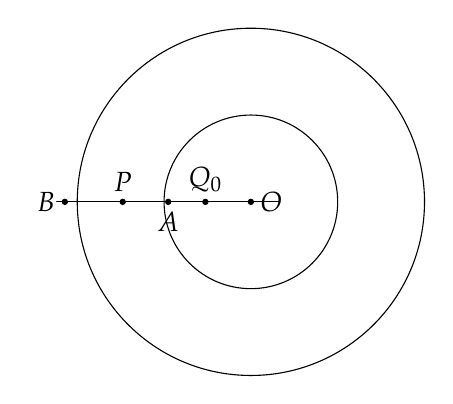
\begin{tikzpicture}[scale=1.05, line cap=round, line join=round]
  \coordinate (O) at (0,0);
  \coordinate (B) at (-2.25,0);
  \coordinate (P) at (-1.55,0);
  \coordinate (A) at (-1.0,0);
  \coordinate (Q0) at (-0.55,0);
  \draw (O) circle (1.05);
  \draw (O) circle (2.1);
  \draw (-2.35,0) -- (0.35,0);
  \foreach \pt/\lab/\pos in {B/B/left,P/P/above,A/A/below,Q0/Q_0/above,O/O/right} {
    \fill (\pt) circle (1.1pt) node[\pos] {$\lab$};
  }
\end{tikzpicture}

Fig. 14.
\end{center}

\[
OP_s.OQ_s=b^2,
\]
and $OP_s.OQ_{s-1}=b^2e^{2\varpi}$, also
$OQ_0=be^{-u}$, $OP_1=be^{u+2\varpi}$,
$OQ_1=be^{-(u+2\varpi)}$, \&c. Hence
$OP_s=be^{u+2s\varpi}$, $OQ_s=be^{-(u+2s\varpi)}$.
If the charge of $P$ is denoted by $P$, then

\[
P_s=Pe^{s\varpi},\qquad Q_s=-Pe^{-(u+s\varpi)}.
\]

Next, let $Q'_1$ be the image of $P$ in the second sphere, $P'_1$ that
of $Q'_1$ in the first, \&c.,

\[
OQ'_1=be^{2\varpi-u},
\]
$OP'_1=be^{u-2\varpi}$, $OQ'_2=be^{4\varpi-u}$,
$OP'_2=be^{u-4\varpi}$; $OP'_s=be^{u-2s\varpi}$,
$OQ'_s=be^{2s\varpi-u}$, $P'_s=Pe^{s\varpi-u}$.

Of these images all the $P$'s are positive, and all the $Q$'s
negative, all the $P$'s and $Q$'s belong to the first sphere, and all
the $P'$'s and $Q'$'s to the second.

The images within the first sphere form a converging series, the sum
of which is

\[
-P\frac{e^{\varpi-u}-1}{e^{\varpi}-1}.
\]

This therefore is the quantity of electricity on the first or interior
sphere. The images outside the second sphere form a diverging series,
but the surface-integral of each with respect to the spherical surface
is zero. The charge of electricity on the exterior spherical surface is
therefore

\[
P\left(\frac{e^{\varpi-u}-1}{e^\varpi-1}-1\right)
=-P\frac{e^\varpi-e^{\varpi-u}}{e^\varpi-1}.
\]

If we substitute for these expressions their values in terms of $OA$,
$OB$, and $OP$, we find

charge on
\[
A=-P\frac{OA}{OP}\frac{PB}{AB},
\]
charge on $B=-P\frac{OB}{OP}\frac{AP}{AB}$.

If we suppose the radii of the spheres to become infinite, the case
becomes that of a point placed between two parallel planes $A$ and $B$.
In this case these expressions become

charge on
\[
A=-P\frac{PB}{AB},
\]

charge on
\[
B=-P\frac{AP}{AB}.
\]

172.] In order to pass from this case to that of any two spheres

not intersecting each other, we begin by finding the two common inverse
points $O$, $O'$ through which all circles pass that are orthogonal to
both spheres. Then, inverting the system with respect to either of
these points, the spheres become concentric, as in the first case.

\begin{center}
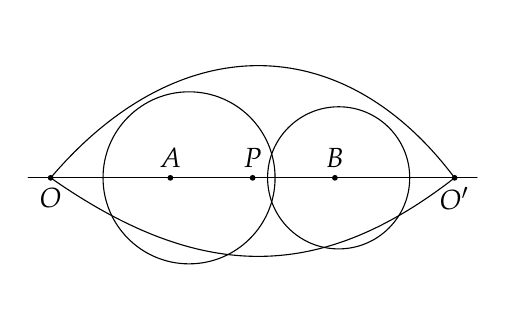
\begin{tikzpicture}[scale=0.95, line cap=round, line join=round]
  \coordinate (Ol) at (-2.7,0);
  \coordinate (A) at (-1.1,0);
  \coordinate (P) at (0,0);
  \coordinate (B) at (1.1,0);
  \coordinate (Or) at (2.7,0);
  \draw (-3.0,0) -- (3.0,0);
  \draw (-0.85,0) circle (1.15);
  \draw (1.15,0) circle (0.95);
  \draw (-2.7,0) .. controls (-1.0,2.0) and (1.2,2.0) .. (2.7,0);
  \draw (-2.7,0) .. controls (-0.7,-1.4) and (0.9,-1.4) .. (2.7,0);
  \foreach \pt/\lab/\pos in {Ol/O/below,A/A/above,P/P/above,B/B/above,Or/O'/below} {
    \fill (\pt) circle (1.1pt) node[\pos] {$\lab$};
  }
\end{tikzpicture}

Fig. 15.
\end{center}

The radius $OAPB$ on which the successive images lie becomes an arc of
a circle through $O$ and $O'$, and the ratio of $O'P$ to $OP$ is

equal to $Ce^u$ where $C$ is a numerical quantity which for simplicity
we may make equal to unity.

We therefore put

\[
u=\log\frac{O'P}{OP},\quad
a=\log\frac{O'A}{OA},\quad
\beta=\log\frac{O'B}{OB}.
\]

Let

\[
\beta - a = \varpi, \qquad u - a = \theta.
\]

Then all the successive images of $P$ will lie on the arc $OAPBO'$.

The position of the image of $P$ in $A$ is $Q_0$ where

\[
u(Q_0)=\log\frac{O'Q}{OQ}=2a-u.
\]

That of $Q_0$ in $B$ is $P_1$ where

\[
u(P_1)=\log\frac{O'P_1}{OP_1}=u+2\varpi.
\]

Similarly

\[
u(P_s)=u+2s\varpi,\qquad
u(Q_s)=2a-u-2s\varpi.
\]

In the same way if the successive images of $P$ in $B$, $A$, $B$,
\&c. are $Q'_0$, $P'_1$, $Q'_1$, \&c.,

\[
u(Q'_0)=2\beta-u,\qquad u(P'_1)=u-2\varpi;
\]
\[
u(P'_s)=u-2s\varpi,\qquad
u(Q'_s)=2\beta-u+2s\varpi.
\]

To find the charge of any image $P_s$ we observe that in the inverted
figure its charge is

\[
P\sqrt{\frac{OP_s}{OP}}.
\]

In the original figure we must multiply this by $O'P_s$. Hence the
charge of $P_s$ in the dipolar figure is

\[
P\sqrt{\frac{OP_s.O'P_s}{OP.O'P}}.
\]

If we make $\xi=\sqrt{OP.O'P}$, and call $\xi$ the parameter of the
point $P$, then we may write

\[
P_s=\frac{\xi_s}{\xi}P,
\]

or the charge of any image is proportional to its parameter.

If we make use of the curvilinear coordinates $u$ and $v$, such that

\[
e^{u+\sqrt{-1}v} = \frac{x+\sqrt{-1}y-k}{x+\sqrt{-1}y+k},
\]

then

\[
x=-\frac{k\sinh u}{\cosh u-\cos v},\qquad
y=\frac{k\sin v}{\cosh u-\cos v};
\]

\[
x^2+(y-k\cot v)^2=k^2\csc^2 v,
\]

\[
(x+k\coth u)^2+y^2=k^2\operatorname{cosech}^2 u,
\]

\[
\cot v=\frac{x^2+y^2-k^2}{2ky},\quad
\coth u=-\frac{x^2+y^2+k^2}{2kx};
\]

\[
\xi=\frac{\sqrt{2k}}{\sqrt{\cosh u-\cos v}}\footnote{In these
expressions we must remember that $2\cosh u=e^u+e^{-u}$,
$2\sinh u=e^u-e^{-u}$, and the other functions of $u$ are derived from
these by the same definitions as the corresponding trigonometrical
functions. The method of applying dipolar coordinates to this case was
given by Thomson in Liouville's Journal for 1847. See Thomson's reprint
of \textit{Electrical Papers}, \S\S 211, 212. In the text I have made
use of the investigation of Prof. Betti, \textit{Nuovo Cimento}, vol.
xx, for the analytical method, but I have retained the idea of
electrical images as used by Thomson in his original investigation,
\textit{Phil. Mag.}, 1853.}.
\]

Since the charge of each image is proportional to its parameter,
$\xi$, and is to be taken positively or negatively according as it is
of the form $P$ or $Q$, we find

\[
P_s=\frac{P\sqrt{\cosh u-\cos v}}
{\sqrt{\cosh(u+2s\varpi)-\cos v}},
\]

\[
Q_s=-\frac{P\sqrt{\cosh u-\cos v}}
{\sqrt{\cosh(2a-u-2s\varpi)-\cos v}},
\]

\[
P'_s=\frac{P\sqrt{\cosh u-\cos v}}
{\sqrt{\cosh(u-2s\varpi)-\cos v}},
\]

\[
Q'_s=-\frac{P\sqrt{\cosh u-\cos v}}
{\sqrt{\cosh(2\beta-u+2s\varpi)-\cos v}}.
\]

We have now obtained the positions and charges of the two infinite
series of images. We have next to determine the total charge on the
sphere $A$ by finding the sum of all the images within it which are of
the form $Q$ or $P'$. We may write this

\[
P\sqrt{\cosh u-\cos v}\sum_{s=1}^{\infty}
\frac{1}{\sqrt{\cosh(u-2s\varpi)-\cos v}},
\]

\[
-P\sqrt{\cosh u-\cos v}\sum_{s=0}^{\infty}
\frac{1}{\sqrt{\cosh(2a-u-2s\varpi)-\cos v}}.
\]

In the same way the total induced charge on B is

\[
P\sqrt{\cosh u-\cos v}\sum_{s=1}^{\infty}
\frac{1}{\sqrt{\cosh(u+2s\varpi)-\cos v}},
\]

\[
-P\sqrt{\cosh u-\cos v}\sum_{s=0}^{\infty}
\frac{1}{\sqrt{\cosh(2\beta-u+2s\varpi)-\cos v}}.
\]

173.] We shall apply these results to the determination of the
coefficients of capacity and induction of two spheres whose radii are
$a$ and $b$, and the distance of whose centres is $c$.

In this case

\[
k = \frac{\sqrt{a^4 + b^4 + c^4 - 2b^2c^2 - 2c^2a^2 - 2a^2b^2}}{2c};
\]
  
\[
\sinh a=\frac{k}{a},\qquad \sinh\beta=\frac{k}{b}.
\]

Let the sphere $A$ be at potential unity, and the sphere $B$ at
potential zero.

Then the successive images of a charge $a$ placed at the centre of the
sphere $A$ will be those of the actual distribution of electricity. All
the images will lie on the axis between the poles and the centres of
the spheres.

The values of $u$ and $v$ for the centre of the sphere $A$ are

\[
u=2a, \qquad v=0.
\]

Hence we must substitute $a$ or $k\frac{1}{\sinh a}$ for $P$, and $2a$
for $u$, and $v=0$ in the equations, remembering that $P$ itself forms
part of the charge of $A$. We thus find for the coefficient of capacity
of $A$

\[
q_{aa}=k\sum_{s=0}^{\infty}\frac{1}{\sinh(s\varpi-a)},
\]

for the coefficient of induction of A on B or of B on A

\[
q_{ab}=-k\sum_{s=1}^{\infty}\frac{1}{\sinh s\varpi},
\]

and for the coefficient of capacity of B

\[
q_{bb}=k\sum_{s=0}^{\infty}\frac{1}{\sinh(\beta+s\varpi)}.
\]

To calculate these quantities in terms of $a$ and $b$, the radii of
the spheres, and of $c$ the distance between their centres, we make use
of the following quantities

\[
p = e^{a} = \sqrt{\frac{k^2}{a^2} + 1} - \frac{k}{a},
\]

\[
q = e^{\beta} = \sqrt{\frac{k^2}{b^2} + 1} + \frac{k}{b},
\]

\[
\frac{q}{p}=r=e^\varpi
=\left(\sqrt{\frac{k^2}{a^2}+1}+\frac{k}{a}\right)
\left(\sqrt{\frac{k^2}{b^2}+1}+\frac{k}{b}\right).
\]

We may now write the hyperbolic sines in terms of $p$, $q$, $r$; thus

\[
q_{aa}=\sum_{s=0}^{\infty}\frac{2k}{\frac{r^s}{p}-\frac{p}{r^s}},
\]

\[
q_{ab}=-\sum_{s=1}^{\infty}\frac{2k}{r^s-\frac{1}{r^s}},
\]

\[
q_{bb}=\sum_{s=0}^{\infty}\frac{2k}{qr^s-\frac{1}{qr^s}}.
\]

Proceeding to the actual calculation we find, either by this process or
by the direct calculation of the successive images as shewn in Sir W.
Thomson's paper, which is more convenient for the earlier part of the
series,

\[
\begin{aligned}
q_{aa} &= a+\frac{a^2b}{c^2-b^2}
 +\frac{a^3b^2}{(c^2-b^2+ac)(c^2-b^2-ac)}+\&c.,\\
q_{ab} &= -\frac{ab}{c}-\frac{a^2b^2}{c(c^2-a^2-b^2)}
 -\frac{a^3b^3}{c(c^2-a^2-b^2+ab)(c^2-a^2-b^2-ab)}-\&c.,\\
q_{bb} &= b+\frac{ab^2}{c^2-a^2}
 +\frac{a^2b^3}{(c^2-a^2+bc)(c^2-a^2-bc)}+\&c.
\end{aligned}
\]

174.] We have then the following equations to determine the charges
$E_a$ and $E_b$ of the two spheres when electrified to potentials
$V_a$ and $V_b$ respectively,

\[
E_a = V_a q_{aa} + V_b q_{ab},
\]

\[
E_b = V_a q_{ab} + V_b q_{bb}.
\]
If we put 
\[
q_{aa} q_{bb} - q_{ab}^2 = D = \frac{1}{D'},
\]
and 
\[
p_{aa} = q_{bb} D', \quad p_{ab} = -q_{ab} D', \quad p_{bb} = q_{aa} D',
\]
whence 
\[
p_{aa} p_{bb} - p_{ab}^2 = D';
\]

then the equations to determine the potentials in terms of the charges
are
\[
V_a=p_{aa}E_a+p_{ab}E_b,\qquad
V_b=p_{ab}E_a+p_{bb}E_b,
\]

and  $p_{aa}$ ,  $p_{ab}$ , and  $p_{bb}$  are the coefficients of potential.

The total energy of the system is, by Art. 85,

\[
\begin{aligned}
Q &= \frac{1}{2}(E_aV_a+E_bV_b),\\
  &= \frac{1}{2}(V_a^2q_{aa}+2V_aV_bq_{ab}+V_b^2q_{bb}),\\
  &= \frac{1}{2}(E_a^2p_{aa}+2E_aE_bp_{ab}+E_b^2p_{bb}).
\end{aligned}
\]

The repulsion between the spheres is therefore, by Arts. 92, 93,

\[
\begin{aligned}
F &= \frac{1}{2}\left\{
V_a^2\frac{dq_{aa}}{dc}+2V_aV_b\frac{dq_{ab}}{dc}
  +V_b^2\frac{dq_{bb}}{dc}\right\},\\
  &= -\frac{1}{2}\left\{
E_a^2\frac{dp_{aa}}{dc}+2E_aE_b\frac{dp_{ab}}{dc}
  +E_b^2\frac{dp_{bb}}{dc}\right\},
\end{aligned}
\]

where $c$ is the distance between the centres of the spheres.

Of these two expressions for the repulsion, the first, which expresses
it in terms of the potentials of the spheres and the variations of the
coefficients of capacity and induction, is the most convenient for
calculation.

We have therefore to differentiate the $q$'s with respect to $c$.
These quantities are expressed as functions of $k$, $a$, $\beta$, and
$\varpi$, and must be differentiated on the supposition that $a$ and
$b$ are constant. From the equations

\[
k=a\sinh a=b\sinh\beta
=c\frac{\sinh a\sinh\beta}{\sinh\varpi},
\]
we find
\[
\frac{da}{dc}=\frac{\sinh a\cosh\beta}{k\sinh\varpi},
\]

\[
\frac{d\beta}{dc}=\frac{\cosh a\sinh\beta}{k\sinh\varpi},
\]

\[
\frac{d\varpi}{dc}=\frac{1}{k},
\]

\[
\frac{dk}{dc}=\frac{\cosh a\cosh\beta}{\sinh\varpi};
\]

whence we find

\[
\frac{dq_{aa}}{dc}
=\frac{\cosh a\cosh\beta}{\sinh\varpi}\frac{q_{aa}}{k}
-\sum_{s=0}^{\infty}
\frac{(sc-a\cosh\beta)\cosh(s\varpi-a)}
{c\{\sinh(s\varpi-a)\}^2},
\]

\[
\frac{dq_{ab}}{dc}
=\frac{\cosh a\cosh\beta}{\sinh\varpi}\frac{q_{ab}}{k}
+\sum_{s=1}^{\infty}\frac{s\cosh s\varpi}{(\sinh s\varpi)^2},
\]

\[
\frac{dq_{bb}}{dc}
=\frac{\cosh a\cosh\beta}{\sinh\varpi}\frac{q_{bb}}{k}
-\sum_{s=0}^{\infty}
\frac{(sc+b\cosh a)\cosh(\beta+s\varpi)}
{c\{\sinh(\beta+s\varpi)\}^2}.
\]

Sir William Thomson has calculated the force between two spheres of
equal radius separated by any distance less than the diameter of one of
them. For greater distances it is not necessary to use more than two or
three of the successive images.

The series for the differential coefficients of the $q$'s with respect
to $c$ are easily obtained by direct differentiation

% batch_0258
\setcounter{footnote}{0}
\[
\begin{split}
\frac{dq_{aa}}{dc}
&= -\frac{2a^2bc}{(c^2-b^2)^2}
   -\frac{2a^3b^2c(2c^2-2b^2-a^2)}
          {(c^2-b^2+ac)^2(c^2-b^2-ac)^2}
   - \&c.,\\
\frac{dq_{ab}}{dc}
&= \frac{ab}{c^2}
   +\frac{a^2b^2(3c^2-a^2-b^2)}
          {c^2(c^2-a^2-b^2)}\\
&\qquad
   +\frac{a^3b^3\{(5c^2-a^2-b^2)(c^2-a^2-b^2)-a^2b^2\}}
          {c^2(c^2-a^2-b^2+ab)^2(c^2-a^2-b^2-ab)^2}
   - \&c.,\\
\frac{dq_{bb}}{dc}
&= -\frac{2ab^2c}{(c^2-a^2)^2}
   -\frac{2a^2b^3c(2c^2-2a^2-b^2)}
          {(c^2-a^2+bc)^2(c^2-a^2-bc)^2}
   - \&c.
\end{split}
\]

\begin{center}
\textit{Distribution of Electricity on Two Spheres in Contact.}
\end{center}

175.] If we suppose the two spheres at potential unity and not influenced by any other point, then, if we invert the system with respect to the point of contact, we shall have two parallel planes, distant $\frac{1}{2a}$ and $\frac{1}{2b}$ from the point of inversion, and electrified by the action of a unit of electricity at that point.

There will be a series of positive images, each equal to unity, at distances $s\left(\frac{1}{a}+\frac{1}{b}\right)$ from the origin, where $s$ may have any integer value from $-\infty$ to $+\infty$.

There will also be a series of negative images each equal to $-1$, the distances of which from the origin, reckoned in the direction of $a$, are $\frac{1}{a}+s\left(\frac{1}{a}+\frac{1}{b}\right)$.

When this system is inverted back again into the form of the two spheres in contact, we have a corresponding series of negative images, the distances of which from the point of contact are of the

form $\frac{1}{s\left(\frac{1}{a}+\frac{1}{b}\right)}$, where $s$ is positive for the sphere $A$ and negative

for the sphere $B$. The charge of each image, when the potential of the spheres is unity, is numerically equal to its distance from the point of contact, and is always negative.

There will also be a series of positive images whose distances from the point of contact measured in the direction of the centre

of $a$, are of the form $\frac{1}{\frac{1}{a}+s\left(\frac{1}{a}+\frac{1}{b}\right)}$.

When $s$ is zero, or a positive integer, the image is in the sphere $A$. When $s$ is a negative integer the image is in the sphere $B$.

The charge of each image is measured by its distance from the origin and is always positive.

The total charge of the sphere $A$ is therefore

\[
E_a
= \sum_{s=0}^{s=\infty}
  \frac{1}{\frac{1}{a}+s\left(\frac{1}{a}+\frac{1}{b}\right)}
  -\frac{ab}{a+b}\sum_{s=1}^{s=\infty}\frac{1}{s}.
\]

Each of these series is infinite, but if we combine them in the form

\[
E_a
= \sum_{s=1}^{s=\infty}
  \frac{a^2b}{s(a+b)\{s(a+b)-a\}}
\]

the series becomes converging.

In the same way we find for the charge of the sphere $B$,

\[
\begin{split}
E_b
&= \sum_{s=1}^{s=\infty}\frac{ab}{s(a+b)-b}
   -\frac{ab}{a+b}\sum_{s=-1}^{s=-\infty}\frac{1}{s},\\
&= \sum_{s=1}^{s=\infty}
   \frac{ab^2}{s(a+b)\{s(a+b)-b\}}.
\end{split}
\]

The values of $E_a$ and $E_b$ are not, so far as I know, expressible in terms of known functions. Their difference, however, is easily expressed, for

\[
E_a-E_b
= \sum_{s=-\infty}^{s=\infty}
  \frac{ab}{b+s(a+b)},
\]
\[
= \frac{\pi ab}{a+b}\cot\frac{\pi b}{a+b}.
\]

When the spheres are equal the charge of each for potential unity is

\[
E_a = a \sum_{s=1}^{s=\infty}\frac{1}{2s(2s-1)},
\]
\[
= a\left(1-\frac{1}{2}+\frac{1}{3}-\frac{1}{4}+\&c.\right),
\]
\[
= a\log_e 2 = 1.0986a.
\]

When the sphere $A$ is very small compared with the sphere $B$ the charge on $A$ is

\[
E_a = \frac{a^2}{b}\sum_{s=1}^{s=\infty}\frac{1}{s^2}
\quad \hbox{approximately};
\]
or
\[
E_a = \frac{\pi^2}{6}\frac{a^2}{b}.
\]

The charge on $B$ is nearly the same as if $A$ were removed, or

\[
E_b=b.
\]

The mean density on each sphere is found by dividing the charge by the surface. In this way we get

\[
\sigma_a = \frac{E_a}{4\pi a^2}=\frac{\pi}{24b},
\]
\[
\sigma_b = \frac{E_b}{4\pi b^2}=\frac{1}{4\pi b},
\]
\[
\sigma_a = \frac{\pi^2}{6}\sigma_b.
\]

Hence, if a very small sphere is made to touch a very large one, the mean density on the small sphere is equal to that on the large sphere multiplied by $\frac{\pi^2}{6}$, or 1.644936.

\begin{center}
\textit{Application of Electrical Inversion to the case of a Spherical Bowl.}
\end{center}

176.] One of the most remarkable illustrations of the power of Sir W. Thomson's method of Electrical Images is furnished by his investigation of the distribution of electricity on a portion of a spherical surface bounded by a small circle. The results of this investigation, without proof, were communicated to M. Liouville and published in his \textit{Journal} in 1847. The complete investigation is given in the reprint of Thomson's \textit{Electrical Papers}, Article XV. I am not aware that a solution of the problem of the distribution of electricity on a finite portion of any curved surface has been given by any other mathematician.

As I wish to explain the method rather than to verify the calculation, I shall not enter at length into either the geometry or the integration, but refer my readers to Thomson's work.

\begin{center}
\textit{Distribution of Electricity on an Ellipsoid.}
\end{center}

177.] It is shewn by a well-known method\footnote{Thomson and Tait's \textit{Natural Philosophy}, \S 520, or Art. 150 of this book.} that the attraction of a shell bounded by two similar and similarly situated and concentric ellipsoids is such that there is no resultant attraction on any point within the shell. If we suppose the thickness of the shell to diminish indefinitely while its density increases, we ultimately arrive at the conception of a surface-density varying as the perpendicular from the centre on the tangent plane, and since the resultant attraction of this superficial distribution on any point within the ellipsoid is zero, electricity, if so distributed on the surface, will be in equilibrium.

Hence, the surface-density at any point of an ellipsoid undisturbed by external influence varies as the distance of the tangent plane from the centre.

\begin{center}
\textit{Distribution of Electricity on a Disk.}
\end{center}

By making two of the axes of the ellipsoid equal, and making the third vanish, we arrive at the case of a circular disk, and at an expression for the surface-density at any point $P$ of such a disk when electrified to the potential $V$ and left undisturbed by external influence. If $\sigma$ be the surface-density on one side of the disk, and if $KPL$ be a chord drawn through the point $P$, then

\[
\sigma = \frac{V}{2\pi^2\sqrt{KP.PL}}.
\]

\begin{center}
\textit{Application of the Principle of Electric Inversion.}
\end{center}

178.] Take any point $Q$ as the centre of inversion, and let $R$ be the radius of the sphere of inversion. Then the plane of the disk becomes a spherical surface passing through $Q$, and the disk itself becomes a portion of the spherical surface bounded by a circle. We shall call this portion of the surface the \textit{bowl}.

If $S'$ is the disk electrified to potential $V'$ and free from external influence, then its electrical image $S$ will be a spherical segment at potential zero, and electrified by the influence of a quantity $V'R$ of electricity placed at $Q$.

We have therefore by the process of inversion obtained the solution of the problem of the distribution of electricity on a bowl or a plane disk when under the influence of an electrified point in the surface of the sphere or plane produced.

\begin{center}
\textit{Influence of an Electrified Point placed on the unoccupied part of the}\\
\textit{Spherical Surface.}
\end{center}

The form of the solution, as deduced by the principles already given and by the geometry of inversion, is as follows:

If $C$ is the central point or pole of the spherical bowl $S$, and if $a$ is the distance from $C$ to any point in the edge of the segment, then, if a quantity $q$ of electricity is placed at a point $Q$ in the surface of the sphere produced, and if the bowl $S$ is maintained at potential zero, the density $\sigma$ at any point $P$ of the bowl will be

\[
\sigma = \frac{1}{2\pi^2}\frac{q}{QP^2}
\sqrt{\frac{CQ^2-a^2}{a^2-CP^2}},
\]

$CQ$, $CP$, and $QP$ being the straight lines joining the points, $C$, $Q$, and $P$.

It is remarkable that this expression is independent of the radius of the spherical surface of which the bowl is a part. It is therefore applicable without alteration to the case of a plane disk.

\begin{center}
\textit{Influence of any Number of Electrified Points.}
\end{center}

Now let us consider the sphere as divided into two parts, one of which, the spherical segment on which we have determined the electric distribution, we shall call the \textit{bowl}, and the other the remainder, or unoccupied part of the sphere on which the influencing point $Q$ is placed.

If any number of influencing points are placed on the remainder of the sphere, the electricity induced by these on any point of the bowl may be obtained by the summation of the densities induced by each separately.

179.] Let the whole of the remaining surface of the sphere be uniformly electrified, the surface-density being $\rho$, then the density at any point of the bowl may be obtained by ordinary integration over the surface thus electrified.

We shall thus obtain the solution of the case in which the bowl is at potential zero, and electrified by the influence of the remaining portion of the spherical surface rigidly electrified with density $\rho$.

Now let the whole system be insulated and placed within a sphere of diameter $f$, and let this sphere be uniformly and rigidly electrified so that its surface-density is $\rho'$.

There will be no resultant force within this sphere, and therefore the distribution of electricity on the bowl will be unaltered, but the potential of all points within the sphere will be increased by a quantity $V$ where

\[
V = \frac{2\pi\rho'}{f}.
\]

Hence the potential at every point of the bowl will now be $V$.

Now let us suppose that this sphere is concentric with the sphere of which the bowl forms a part, and that its radius exceeds that of the latter sphere by an infinitely small quantity.

We have now the case of the bowl maintained at potential $V$ and influenced by the remainder of the sphere rigidly electrified with superficial density $\rho+\rho'$.

180.] We have now only to suppose $\rho+\rho'=0$, and we get the case of the bowl maintained at potential $V$ and free from external influence.

If $\sigma$ is the density on either surface of the bowl at a given point when the bowl is at potential zero, and is influenced by the rest of the sphere electrified to density $\rho$, then, when the bowl is maintained at potential $V$, we must increase the density on the outside of the bowl by $\rho'$, the density on the supposed enveloping sphere.

The result of this investigation is that if $f$ is the diameter of the sphere, $a$ the chord of the radius of the bowl, and $r$ the chord of the distance of $P$ from the pole of the bowl, then the surface-density $\sigma$ on the \textit{inside} of the bowl is

\[
\sigma = \frac{V}{2\pi^2f}
\left\{
\sqrt{\frac{f^2-a^2}{a^2-r^2}}
-\tan^{-1}\sqrt{\frac{f^2-a^2}{a^2-r^2}}
\right\},
\]

and the surface-density on the outside of the bowl at the same point is
\[
\sigma+\frac{V}{2\pi f}.
\]

In the calculation of this result no operation is employed more abstruse than ordinary integration over part of a spherical surface. To complete the theory of the electrification of a spherical bowl we only require the geometry of the inversion of spherical surfaces.

181.] Let it be required to find the surface-density induced at any point of the bowl by a quantity $q$ of electricity placed at a point $Q$, not now in the spherical surface produced.

Invert the bowl with respect to $Q$, the radius of the sphere of inversion being $R$. The bowl $S$ will be inverted into its image $S'$, and the point $P$ will have $P'$ for its image. We have now to determine the density $\sigma'$ at $P'$ when the bowl $S'$ is maintained at potential $V'$, such that $q=V'R$, and is not influenced by any external force.

The density $\sigma$ at the point $P$ of the original bowl is then

\[
\sigma = -\frac{\sigma'R^3}{QP^3},
\]

this bowl being at potential zero, and influenced by a quantity $q$ of electricity placed at $Q$.

The result of this process is as follows:

\begin{center}
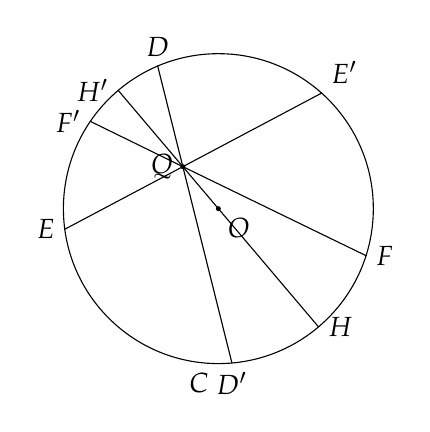
\begin{tikzpicture}[scale=0.82, line cap=round, line join=round]
  \coordinate (O) at (0,0);
  \coordinate (Q) at (-0.55,0.65);
  \coordinate (E) at (-2.38,-0.32);
  \coordinate (Ep) at (1.60,1.79);
  \coordinate (Fp) at (-1.98,1.35);
  \coordinate (F) at (2.29,-0.73);
  \coordinate (D) at (-0.94,2.21);
  \coordinate (Dp) at (0.21,-2.39);
  \coordinate (Hp) at (-1.55,1.83);
  \coordinate (H) at (1.55,-1.83);
  \coordinate (C) at (0,-2.4);
  \draw (O) circle (2.4);
  \draw (E)--(Q)--(Ep);
  \draw (Fp)--(Q)--(F);
  \draw (D)--(Q)--(Dp);
  \draw (Hp)--(Q)--(O)--(H);
  \fill (O) circle (1.1pt) node[below right] {$O$};
  \fill (Q) circle (1.1pt) node[left] {$Q$};
  \node[left] at (E) {$E$};
  \node[above right] at (Ep) {$E'$};
  \node[left] at (Fp) {$F'$};
  \node[right] at (F) {$F$};
  \node[above] at (D) {$D$};
  \node[below] at (Dp) {$D'$};
  \node[left] at (Hp) {$H'$};
  \node[right] at (H) {$H$};
  \node[below left] at (C) {$C$};
\end{tikzpicture}\\
{\small Fig. 16.}
\end{center}

Let the figure represent a section through the centre, $O$, of the sphere, the pole, $C$, of the bowl, and the influencing point $Q$. $D$ is a point which corresponds in the inverted figure to the unoccupied pole of the rim of the bowl, and may be found by the following construction.

Draw through $Q$ the chords $EQE'$ and $FQF'$, then if we suppose the radius of the sphere of inversion to be a mean proportional between the

segments into which a chord is divided at $Q$, $E'F'$ will be the image of $EF$. Bisect the arc $F'CE'$ in $D'$, so that $F'D'=D'E'$, and draw $D'QD$ to meet the sphere in $D$. $D$ is the point required. Also through $O$, the centre of the sphere, and $Q$ draw $HOQH'$ meeting the sphere in $H$ and $H'$. Then if $P$ be any point in the bowl, the surface-density at $P$ on the side which is separated from $Q$ by the completed spherical surface, induced by a quantity $q$ of electricity at $Q$, will be

\[
\sigma =
\frac{q}{2\pi^2}\frac{QH.QH'}{HH'.PQ^3}
\left\{
\frac{PQ}{DQ}\left(\frac{CD^2-a^2}{a^2-CP^2}\right)^{\frac12}
-\tan^{-1}\left[
\frac{PQ}{DQ}\left(\frac{CD^2-a^2}{a^2-CP^2}\right)^{\frac12}
\right]
\right\},
\]

where $a$ denotes the chord drawn from $C$, the pole of the bowl, to the rim of the bowl.

On the side next to $Q$ the surface-density is

\[
\sigma+\frac{q}{2\pi^2}\frac{QH.QH'}{HH'.PQ^3}.
\]

\begin{center}
\Large CHAPTER XII.
\end{center}

\begin{center}
THEORY OF CONJUGATE FUNCTIONS IN TWO DIMENSIONS.
\end{center}

182.] The number of independent cases in which the problem of electrical equilibrium has been solved is very small. The method of spherical harmonics has been employed for spherical conductors, and the methods of electrical images and of inversion are still more powerful in the cases to which they can be applied. The case of surfaces of the second degree is the only one, as far as I know, in which both the equipotential surfaces and the lines of force are known when the lines of force are not plane curves.

But there is an important class of problems in the theory of electrical equilibrium, and in that of the conduction of currents, in which we have to consider space of two dimensions only.

For instance, if throughout the part of the electric field under consideration, and for a considerable distance beyond it, the surfaces of all the conductors are generated by the motion of straight lines parallel to the axis of $z$, and if the part of the field where this ceases to be the case is so far from the part considered that the electrical action of the distant part on the field may be neglected, then the electricity will be uniformly distributed along each generating line, and if we consider a part of the field bounded by two planes perpendicular to the axis of $z$ and at distance unity, the potential and the distribution of electricity will be functions of $x$ and $y$ only.

If $\rho\,dx\,dy$ denotes the quantity of electricity in an element whose base is $dx\,dy$ and height unity, and $\sigma\,ds$ the quantity on an element of area whose base is the linear element $ds$ and height unity, then the equation of Poisson may be written

\[
\frac{d^2V}{dx^2} + \frac{d^2V}{dy^2} + 4\pi\rho = 0.
\]

When there is no free electricity, this is reduced to the equation of Laplace,

\[
\frac{d^2V}{dx^2}+\frac{d^2V}{dy^2}=0.
\]

The general problem of electric equilibrium may be stated as follows:--

A continuous space of two dimensions, bounded by closed curves $C_1$, $C_2$, \&c. being given, to find the form of a function, $V$, such that at these boundaries its value may be $V_1$, $V_2$, \&c. respectively, being constant for each boundary, and that within this space $V$ may be everywhere finite, continuous, and single valued, and may satisfy Laplace's equation.

I am not aware that any perfectly general solution of even this question has been given, but the method of transformation given in Art. 190 is applicable to this case, and is much more powerful than any known method applicable to three dimensions.

The method depends on the properties of conjugate functions of two variables.

\begin{center}
\textit{Definition of Conjugate Functions.}
\end{center}

183.] Two quantities $\alpha$ and $\beta$ are said to be conjugate functions of $x$ and $y$, if $\alpha+\sqrt{-1}\,\beta$ is a function of $x+\sqrt{-1}\,y$.

It follows from this definition that

\begin{equation}\tag{1}
\frac{d\alpha}{dx}=\frac{d\beta}{dy},
\quad \hbox{and}\quad
\frac{d\alpha}{dy}+\frac{d\beta}{dx}=0;
\end{equation}

\begin{equation}\tag{2}
\frac{d^2\alpha}{dx^2}+\frac{d^2\alpha}{dy^2}=0,
\qquad
\frac{d^2\beta}{dx^2}+\frac{d^2\beta}{dy^2}=0.
\end{equation}

Hence both functions satisfy Laplace's equation. Also

\begin{equation}\tag{3}
\frac{d\alpha}{dx}\frac{d\beta}{dy}
-\frac{d\alpha}{dy}\frac{d\beta}{dx}
=\left(\frac{d\alpha}{dx}\right)^2
 +\left(\frac{d\alpha}{dy}\right)^2
=\left(\frac{d\beta}{dx}\right)^2
 +\left(\frac{d\beta}{dy}\right)^2
=R^2.
\end{equation}

If $x$ and $y$ are rectangular coordinates, and if $ds_1$ is the intercept of the curve ($\beta={}$constant) between the curves $\alpha$ and $\alpha+d\alpha$, and $ds_2$ the intercept of $\alpha$ between the curves $\beta$ and $\beta+d\beta$, then

\begin{equation}\tag{4}
\frac{ds_1}{d\alpha}=\frac{ds_2}{d\beta}=\frac{1}{R},
\end{equation}

and the curves intersect at right angles.

If we suppose the potential $V=V_0+k\alpha$, where $k$ is some constant, then $V$ will satisfy Laplace's equation, and the curves ($\alpha$) will be equipotential curves. The curves ($\beta$) will be lines of force, and the surface-integral of a surface whose projection on the plane of $xy$ is the curve $AB$ will be $k(\beta_B-\beta_A)$, where $\beta_A$ and $\beta_B$ are the values of $\beta$ at the extremities of the curve.

If a series of curves corresponding to values of $\alpha$ in arithmetical progression is drawn on the plane, and another series corresponding to a series of values of $\beta$ having the same common difference, then the two series of curves will everywhere intersect at right angles, and, if the common difference is small enough, the elements into which the plane is divided will be ultimately little squares, whose sides, in different parts of the field, are in different directions and of different magnitude, being inversely proportional to $R$.

If two or more of the equipotential lines ($\alpha$) are closed curves enclosing a continuous space between them, we may take these for the surfaces of conductors at potentials $(V_0+k\alpha_1)$, $(V_0+k\alpha_2)$, \&c. respectively. The quantity of electricity upon any one of these between the lines of force $\beta_1$ and $\beta_2$ will be $\frac{k}{4\pi}(\beta_2-\beta_1)$.

The number of equipotential lines between two conductors will therefore indicate their difference of potential, and the number of lines of force which emerge from a conductor will indicate the

quantity of electricity upon it. We must next state some of the most important theorems relating to conjugate functions, and in proving them we may use either the equations (1), containing the differential coefficients, or the original definition, which makes use of imaginary symbols.

184.] \textsc{Theorem I.} \textit{If $x'$ and $y'$ are conjugate functions with respect to $x$ and $y$, and if $x''$ and $y''$ are also conjugate functions with respect to $x$ and $y$, then the functions $x'+x''$ and $y'+y''$ will be conjugate functions with respect to $x$ and $y$.}

For
\[
\frac{dx'}{dx}=\frac{dy'}{dy},
\quad \hbox{and}\quad
\frac{dx''}{dx}=\frac{dy''}{dy};
\]
therefore
\[
\frac{d(x'+x'')}{dx}=\frac{d(y'+y'')}{dy}.
\]
Also
\[
\frac{dx'}{dy}=-\frac{dy'}{dx},
\quad \hbox{and}\quad
\frac{dx''}{dy}=-\frac{dy''}{dx};
\]
therefore
\[
\frac{d(x'+x'')}{dy}=-\frac{d(y'+y'')}{dx};
\]

or $x'+x''$ and $y'+y''$ are conjugate with respect to $x$ and $y$.

% batch_0268
\setcounter{footnote}{0}
\begin{center}
\textit{Graphic Representation of a Function which is the Sum of Two}\\
\textit{Given Functions.}
\end{center}

Let a function ($\alpha$) of $x$ and $y$ be graphically represented by a series of curves in the plane of $xy$, each of these curves corresponding to a value of $\alpha$ which belongs to a series of such values increasing by a common difference, $\delta$.

Let any other function, $\beta$, of $x$ and $y$ be represented in the same way by a series of curves corresponding to a series of values of $\beta$ having the same common difference as those of $\alpha$.

Then to represent the function $\alpha+\beta$ in the same way, we must draw a series of curves through the intersections of the two former series from the intersection of the curves ($\alpha$) and ($\beta$) to that of the curves ($\alpha+\delta$) and ($\beta-\delta$), then through the intersection of ($\alpha+2\delta$) and ($\beta-2\delta$), and so on. At each of these points the function will have the same value, namely $\alpha+\beta$. The next curve must be drawn through the points of intersection of $\alpha$ and $\beta+\delta$, of $\alpha+\delta$ and $\beta$, of $\alpha+2\delta$ and $\beta-\delta$, and so on. The function belonging to this curve will be $\alpha+\beta+\delta$.

In this way, when the series of curves ($\alpha$) and the series ($\beta$) are drawn, the series ($\alpha+\beta$) may be constructed. These three series of curves may be drawn on separate pieces of transparent paper, and when the first and second have been properly superposed, the third may be drawn.

The combination of conjugate functions by addition in this way enables us to draw figures of many interesting cases with very little trouble when we know how to draw the simpler cases of which they are compounded. We have, however, a far more powerful method of transformation of solutions, depending on the following theorem.

185.] \textsc{Theorem II.} \textit{If $x''$ and $y''$ are conjugate functions with respect to the variables $x'$ and $y'$, and if $x'$ and $y'$ are conjugate functions with respect to $x$ and $y$, then $x''$ and $y''$ will be conjugate functions with respect to $x$ and $y$.}

For
\[
\frac{dx''}{dx}
= \frac{dx''}{dx'}\frac{dx'}{dx}
 +\frac{dx''}{dy'}\frac{dy'}{dx},
\]
\[
= \frac{dy''}{dy'}\frac{dy'}{dy}
 +\frac{dy''}{dx'}\frac{dx'}{dy},
\]
\[
= \frac{dy''}{dy};
\]

and
\[
\frac{dx''}{dy}
= \frac{dx''}{dx'}\frac{dx'}{dy}
 +\frac{dx''}{dy'}\frac{dy'}{dy},
\]
\[
= -\frac{dy''}{dy'}\frac{dy'}{dx}
 -\frac{dy''}{dx'}\frac{dx'}{dx},
\]
\[
= -\frac{dy''}{dx};
\]

and these are the conditions that $x''$ and $y''$ should be conjugate functions of $x$ and $y$.

This may also be shewn from the original definition of conjugate functions. For $x''+\sqrt{-1}\,y''$ is a function of $x'+\sqrt{-1}\,y'$, and $x'+\sqrt{-1}\,y'$ is a function of $x+\sqrt{-1}\,y$. Hence, $x''+\sqrt{-1}\,y''$ is a function of $x+\sqrt{-1}\,y$.

In the same way we may shew that if $x'$ and $y'$ are conjugate functions of $x$ and $y$, then $x$ and $y$ are conjugate functions of $x'$ and $y'$.

This theorem may be interpreted graphically as follows:

Let $x'$, $y'$ be taken as rectangular coordinates, and let the curves corresponding to values of $x''$ and of $y''$ taken in regular arithmetical series be drawn on paper. A double system of curves will thus be drawn cutting the paper into little squares. Let the paper be also ruled with horizontal and vertical lines at equal intervals, and let these lines be marked with the corresponding values of $x'$ and $y'$.

Next, let another piece of paper be taken in which $x$ and $y$ are made rectangular coordinates and a double system of curves $x'$, $y'$ is drawn, each curve being marked with the corresponding value of $x'$ or $y'$. This system of curvilinear coordinates will correspond, point for point, to the rectilinear system of coordinates $x'$, $y'$ on the first piece of paper.

Hence, if we take any number of points on the curve $x''$ on the first paper, and note the values of $x'$ and $y'$ at these points, and mark the corresponding points on the second paper, we shall find a number of points on the transformed curve $x''$. If we do the same for all the curves $x''$, $y''$ on the first paper, we shall obtain on the second paper a double series of curves $x''$, $y''$ of a different form, but having the same property of cutting the paper into little squares.

186.] \textsc{Theorem III.} \textit{If $V$ is any function of $x'$ and $y'$, and if $x'$ and $y'$ are conjugate functions of $x$ and $y$, then}

\[
\iint\left(\frac{d^2V}{dx^2}+\frac{d^2V}{dy^2}\right)dx\,dy
=
\iint\left(\frac{d^2V}{dx'^2}+\frac{d^2V}{dy'^2}\right)dx'\,dy',
\]

the integration being between the same limits.

For
\[
\frac{dV}{dx}
= \frac{dV}{dx'}\frac{dx'}{dx}
 +\frac{dV}{dy'}\frac{dy'}{dx},
\]

\[
\begin{split}
\frac{d^2V}{dx^2}
&= \frac{d^2V}{dx'^2}\left(\frac{dx'}{dx}\right)^2
 +2\frac{d^2V}{dx'\,dy'}\frac{dx'}{dx}\frac{dy'}{dx}
 +\frac{d^2V}{dy'^2}\left(\frac{dy'}{dx}\right)^2\\
&\qquad
 +\frac{dV}{dx'}\frac{d^2x'}{dx^2}
 +\frac{dV}{dy'}\frac{d^2y'}{dx^2};
\end{split}
\]
and
\[
\begin{split}
\frac{d^2V}{dy^2}
&= \frac{d^2V}{dx'^2}\left(\frac{dx'}{dy}\right)^2
 +2\frac{d^2V}{dx'\,dy'}\frac{dx'}{dy}\frac{dy'}{dy}
 +\frac{d^2V}{dy'^2}\left(\frac{dy'}{dy}\right)^2\\
&\qquad
 +\frac{dV}{dx'}\frac{d^2x'}{dy^2}
 +\frac{dV}{dy'}\frac{d^2y'}{dy^2}.
\end{split}
\]

Adding the last two equations, and remembering the conditions of conjugate functions (1), we find

\[
\begin{split}
\frac{d^2V}{dx^2}+\frac{d^2V}{dy^2}
&= \frac{d^2V}{dx'^2}
   \left\{
   \left(\frac{dx'}{dx}\right)^2
   +\left(\frac{dx'}{dy}\right)^2
   \right\}
 + \frac{d^2V}{dy'^2}
   \left\{
   \left(\frac{dy'}{dx}\right)^2
   +\left(\frac{dy'}{dy}\right)^2
   \right\},\\
&= \left(\frac{d^2V}{dx'^2}+\frac{d^2V}{dy'^2}\right)
   \left(
   \frac{dx'}{dx}\frac{dy'}{dy}
   -\frac{dx'}{dy}\frac{dy'}{dx}
   \right).
\end{split}
\]

Hence

\[
\iint\left(\frac{d^2V}{dx^2}+\frac{d^2V}{dy^2}\right)dx\,dy
=
\iint\left(\frac{d^2V}{dx'^2}+\frac{d^2V}{dy'^2}\right)
\left(
\frac{dx'}{dx}\frac{dy'}{dy}
-\frac{dx'}{dy}\frac{dy'}{dx}
\right)dx\,dy,
\]

\[
= \iint\left(\frac{d^2V}{dx'^2}+\frac{d^2V}{dy'^2}\right)dx'\,dy'.
\]

If $V$ is a potential, then, by Poisson's equation

\[
\frac{d^2V}{dx^2}+\frac{d^2V}{dy^2}+4\pi\rho=0,
\]

and we may write the result

\[
\iint \rho\,dx\,dy = \iint \rho'\,dx'\,dy',
\]

or the quantity of electricity in corresponding portions of two systems is the same if the coordinates of one system are conjugate functions of those of the other.

\begin{center}
\textit{Additional Theorems on Conjugate Functions.}
\end{center}

187.] \textsc{Theorem IV.} \textit{If $x_1$ and $y_1$, and also $x_2$ and $y_2$, are conjugate functions of $x$ and $y$, then, if}

\[
X=x_1x_2-y_1y_2,\qquad
Y=x_1y_2+x_2y_1,
\]

\textit{$X$ and $Y$ will be conjugate functions of $x$ and $y$.}

For
\[
X+\sqrt{-1}\,Y
=(x_1+\sqrt{-1}\,y_1)(x_2+\sqrt{-1}\,y_2).
\]

\textsc{Theorem V.} \textit{If $\phi$ be a solution of the equation}

\[
\frac{d^2\phi}{dx^2}+\frac{d^2\phi}{dy^2}=0,
\]
\textit{and if}
\[
2R=\log\left\{
\left(\frac{d\phi}{dx}\right)^2
+\left(\frac{d\phi}{dy}\right)^2
\right\},
\qquad
\Theta=\tan^{-1}
\frac{\frac{d\phi}{dx}}{\frac{d\phi}{dy}},
\]

\textit{$R$ and $\Theta$ will be conjugate functions of $x$ and $y$.}

For $R$ and $\Theta$ are conjugate functions of $\frac{d\phi}{dx}$ and $\frac{d\phi}{dy}$, and these are conjugate functions of $x$ and $y$.

\begin{center}
\textsc{Example I.}--\textit{Inversion.}
\end{center}

188.] As an example of the general method of transformation let us take the case of inversion in two dimensions.

If $O$ is a fixed point in a plane, and $OA$ a fixed direction, and if $r=OP=ae^\rho$, and $\theta=AOP$, and if $x$, $y$ are the rectangular coordinates of $P$ with respect to $O$,

\begin{equation}\tag{5}
\begin{gathered}
\rho=\log\frac{1}{a}\sqrt{x^2+y^2},
\qquad
\theta=\tan^{-1}\frac{y}{x},\\
x=ae^\rho\cos\theta,
\qquad
y=ae^\rho\sin\theta,
\end{gathered}
\end{equation}

$\rho$ and $\theta$ are conjugate functions of $x$ and $y$.

If $\rho'=n\rho$ and $\theta'=n\theta$, $\rho'$ and $\theta'$ will be conjugate functions of $\rho$ and $\theta$. In the case in which $n=-1$ we have

\begin{equation}\tag{6}
r'=\frac{a^2}{r},\qquad \theta'=-\theta,
\end{equation}

which is the case of ordinary inversion combined with turning the figure $180^\circ$ round $OA$.

\begin{center}
\textit{Inversion in Two Dimensions.}
\end{center}

In this case if $r$ and $r'$ represent the distances of corresponding points from $O$, $e$ and $e'$ the total electrification of a body, $S$ and $S'$ superficial elements, $V$ and $V'$ solid elements, $\sigma$ and $\sigma'$ surface-densities, $\rho$ and $\rho'$ volume densities, $\phi$ and $\phi'$ corresponding potentials,

\begin{equation}\tag{7}
\left.
\begin{gathered}
\frac{r'}{r}=\frac{S'}{S}=\frac{a^2}{r^2}=\frac{r'^2}{a^2},
\qquad
\frac{V'}{V}=\frac{a^4}{r^4}=\frac{r'^4}{a^4},\\
\frac{e'}{e}=1,\qquad
\frac{\sigma'}{\sigma}=\frac{r^2}{a^2}=\frac{a^2}{r'^2},
\qquad
\frac{\rho'}{\rho}=\frac{r^4}{a^4}=\frac{a^4}{r'^4},\\
\frac{\phi'}{\phi}=1.
\end{gathered}
\right\}
\end{equation}

\begin{center}
\textsc{Example II.}--\textit{Electric Images in Two Dimensions.}
\end{center}

189.] Let $A$ be the centre of a circle of radius $AQ=b$, and let $E$ be a charge at $A$, then the potential at any point $P$ is

\begin{equation}\tag{8}
\phi = 2E \log \frac{b}{AP};
\end{equation}

and if the circle is a section of a hollow conducting cylinder, the surface-density at any point $Q$ is $-\frac{E}{2\pi b}$.

\begin{center}
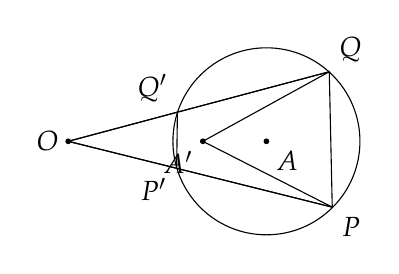
\begin{tikzpicture}[scale=0.95, line cap=round, line join=round]
  \coordinate (O) at (-1.45,0);
  \coordinate (Ap) at (0.35,0);
  \coordinate (A) at (1.20,0);
  \coordinate (Qp) at (0.01,0.39);
  \coordinate (Q) at (2.04,0.93);
  \coordinate (Pp) at (0.00,-0.36);
  \coordinate (P) at (2.08,-0.88);
  \draw (A) circle (1.25);
  \draw (O)--(Q)--(P)--cycle;
  \draw (O)--(Qp)--(Q);
  \draw (O)--(Pp)--(P);
  \draw (Ap)--(Q);
  \draw (Ap)--(P);
  \draw (Qp)--(Pp);
  \fill (O) circle (1.1pt) node[left] {$O$};
  \fill (Ap) circle (1.1pt) node[below left] {$A'$};
  \fill (A) circle (1.1pt) node[below right] {$A$};
  \node[above left] at (Qp) {$Q'$};
  \node[above right] at (Q) {$Q$};
  \node[below left] at (Pp) {$P'$};
  \node[below right] at (P) {$P$};
\end{tikzpicture}\\
{\small Fig. 17.}
\end{center}

Invert the system with respect to a point $O$, making

\[
AO=mb,\qquad a^2=(m^2-1)b^2;
\]

then we have a charge at $A'$ equal to that at $A$, where $AA'=\frac{b}{m}$.

The density at $Q'$ is

\[
-\frac{E}{2\pi b}\frac{b^2-AA'^2}{A'Q'^2},
\]

and the potential at any point $P'$ within the circle is

\begin{equation}\tag{9}
\begin{split}
\phi'=\phi
&= 2E(\log b-\log AP),\\
&= 2E(\log OP'-\log A'P'-\log m).
\end{split}
\end{equation}

This is equivalent to a combination of a charge $E$ at $A'$, and a charge $-E$ at $O$, which is the image of $A'$, with respect to the circle. The imaginary charge at $O$ is equal and opposite to that at $A'$.

If the point $P'$ is defined by its polar coordinates referred to the centre of the circle, and if we put

\begin{equation}\tag{10}
\rho=\log r-\log b,\quad
\hbox{and}\quad
\rho_0=\log AA'-\log b,
\qquad
A'P'=be^\rho,\quad
AA'=be^{\rho_0},\quad
AO=be^{-\rho_0};
\end{equation}

and the potential at the point  $(\rho, \theta)$  is

\begin{equation}\tag{11}
\begin{split}
\phi
&= E\log\left(e^{-2\rho_0}-2e^{-\rho_0}e^\rho\cos\theta+e^{2\rho}\right)\\
&\quad
-E\log\left(e^{2\rho_0}-2e^{\rho_0}e^\rho\cos\theta+e^{2\rho}\right)
+2E\rho_0.
\end{split}
\end{equation}

This is the potential at the point $(\rho,\theta)$ due to a charge $E$, placed at the point $(\rho_0,0)$, with the condition that when $\rho=0$, $\phi=0$.

In this case $\rho$ and $\theta$ are the conjugate functions in equations (5): $\rho$ is the logarithm of the ratio of the radius vector of a point to the radius of the circle, and $\theta$ is an angle.

The centre is the only singular point in this system of coordinates, and the line-integral of $\int \frac{d\theta}{ds}\,ds$ round a closed curve is zero or $2\pi$, according as the closed curve excludes or includes the centre.

\begin{center}
\textsc{Example III.}--\textit{Neumann's Transformation of this Case}\footnote{See Crelle's \textit{Journal}, 1861.}
\end{center}

190.] Now let $\alpha$ and $\beta$ be any conjugate functions of $x$ and $y$, such that the curves ($\alpha$) are equipotential curves, and the curves ($\beta$) are lines of force due to a system consisting of a charge of half a unit at the origin, and an electrified system disposed in any manner at a certain distance from the origin.

Let us suppose that the curve for which the potential is $\alpha_0$ is a closed curve, such that no part of the electrified system except the half-unit at the origin lies within this curve.

Then all the curves ($\alpha$) between this curve and the origin will be closed curves surrounding the origin, and all the curves ($\beta$) will meet in the origin, and will cut the curves ($\alpha$) orthogonally.

The coordinates of any point within the curve ($\alpha_0$) will be determined by the values of $\alpha$ and $\beta$ at that point, and if the point travels round one of the curves $\alpha$ in the positive direction, the value of $\beta$ will increase by $2\pi$ for each complete circuit.

If we now suppose the curve ($\alpha_0$) to be the section of the inner surface of a hollow cylinder of any form maintained at potential zero under the influence of a charge of linear density $E$ on a line of which the origin is the projection, then we may leave the external electrified system out of consideration, and we have for the potential at any point ($\alpha$) within the curve

\begin{equation}\tag{12}
\phi = 2E(\alpha - \alpha_0),
\end{equation}

and for the quantity of electricity on any part of the curve $\alpha_0$ between the points corresponding to $\beta_1$ and $\beta_2$,

\begin{equation}\tag{13}
Q = 2E(\beta_1-\beta_2).
\end{equation}

If in this way, or in any other, we have determined the distribution of potential for the case of a given curve of section when the charge is placed at a given point taken as origin, we may pass to the case in which the charge is placed at any other point by an application of the general method of transformation.

Let the values of $\alpha$ and $\beta$ for the point at which the charge is placed be $\alpha_1$ and $\beta_1$, then substituting in equation (11) $\alpha-\alpha_0$ for $\rho$, and $\beta-\beta_1$ for $\theta$, we find for the potential at any point whose coordinates are $\alpha$ and $\beta$,

\begin{equation}\tag{14}
\begin{split}
\phi
&= E\log\left(1-2e^{\alpha-\alpha_1}\cos(\beta-\beta_1)+e^{2(\alpha-\alpha_1)}\right)\\
&\quad
-E\log\left(1-2e^{\alpha+\alpha_1-2\alpha_0}\cos(\beta-\beta_1)
+e^{2(\alpha+\alpha_1-2\alpha_0)}\right)
+2E(\alpha_1-\alpha_0).
\end{split}
\end{equation}

This expression for the potential becomes zero when $\alpha=\alpha_0$, and is finite and continuous within the curve $\alpha_0$ except at the point $\alpha_1\beta_1$, at which point the first term becomes infinite, and in its immediate neighbourhood is ultimately equal to $2E\log r'$, where $r'$ is the distance from that point.

We have therefore obtained the means of deducing the solution of Green's problem for a charge at any point within a closed curve when the solution for a charge at any other point is known.

The charge induced upon an element of the curve $\alpha_0$ between the points $\beta$ and $\beta+d\beta$ by a charge $E$ placed at the point $\alpha_1\beta_1$ is

\begin{equation}\tag{15}
\frac{E}{2\pi}
\frac{1-e^{2(\alpha_1-\alpha_0)}}
{1-2e^{(\alpha_1-\alpha_0)}\cos(\beta-\beta_1)+e^{2(\alpha_1-\alpha_0)}}\,d\beta.
\end{equation}

From this expression we may find the potential at any point $\alpha_1\beta_1$ within the closed curve, when the value of the potential at every point of the closed curve is given as a function of $\beta$, and there is no electrification within the closed curve.

For, by Theorem II of Chap. III, the part of the potential at $\alpha_1\beta_1$, due to the maintenance of the portion $d\beta$ of the closed curve at the potential $V$, is $nV$, where $n$ is the charge induced on $d\beta$ by unit of electrification at $\alpha_1\beta_1$. Hence, if $V$ is the potential at a point on the closed curve defined as a function of $\beta$, and $\phi$ the potential at the point $\alpha$, $\beta$, within the closed curve, there being no electrification within the curve,

\begin{equation}\tag{16}
\phi = \frac{1}{2\pi}\int_0^{2\pi}
\frac{\left(1-e^{2(\alpha_1-\alpha_0)}\right)V\,d\beta}
{1-2e^{(\alpha_1-\alpha_0)}\cos(\beta-\beta_1)+e^{2(\alpha_1-\alpha_0)}}.
\end{equation}

\begin{center}
\textsc{Example IV.}--\textit{Distribution of Electricity near an Edge of a}\\
\textit{Conductor formed by Two Plane Faces.}
\end{center}

191.] In the case of an infinite plane face of a conductor charged with electricity to the surface-density $\sigma_0$, we find for the potential at a distance $y$ from the plane

\[
V=C-4\pi\sigma_0y,
\]

where $C$ is the value of the potential of the conductor itself.

Assume a straight line in the plane as a polar axis, and transform into polar coordinates, and we find for the potential

\[
V=C-4\pi\sigma_0ae^\rho\sin\theta,
\]

and for the quantity of electricity on a parallelogram of breadth unity, and length $ae^\rho$ measured from the axis

\[
E=\sigma_0ae^\rho.
\]

Now let us make $\rho=n\rho'$ and $\theta=n\theta'$, then, since $\rho'$ and $\theta'$ are conjugate to $\rho$ and $\theta$, the equations

\[
V=C-4\pi\sigma_0ae^{n\rho'}\sin n\theta'
\]

\[
E=\sigma_0ae^{n\rho'}
\]

express a possible distribution of electricity and of potential.

If we write $r$ for $ae^{\rho'}$, $r$ will be the distance from the axis, and $\theta$ the angle, and we shall have

\[
V=C-4\pi\sigma_0\frac{r^n}{a^{n-1}}\sin n\theta,
\]

\[
E=\sigma_0\frac{r^n}{a^{n-1}}.
\]

$V$ will be equal to $C$ whenever $n\theta=\pi$ or a multiple of $\pi$.

Let the edge be a salient angle of the conductor, the inclination of the faces being $a$, then the angle of the dielectric is $2\pi-a$, so that when $\theta=2\pi-a$ the point is in the other face of the conductor. We must therefore make

\[
n(2\pi-a)=\pi,
\qquad
n=\frac{\pi}{2\pi-a}.
\]

Then
\[
V=C-4\pi\sigma_0a
\left(\frac{r}{a}\right)^{\frac{\pi}{2\pi-a}}
\sin\frac{\pi\theta}{2\pi-a},
\]
\[
E=\sigma_0a
\left(\frac{r}{a}\right)^{\frac{\pi}{2\pi-a}}.
\]

The surface-density $\sigma$ at any distance $r$ from the edge is

\[
\sigma=\frac{dE}{dr}
=\frac{\pi}{2\pi-a}\sigma_0
\left(\frac{r}{a}\right)^{\frac{a-\pi}{2\pi-a}}.
\]

When the angle is a salient one $a$ is less than $\pi$, and the surface-density varies according to some inverse power of the distance from the edge, so that at the edge itself the density becomes infinite, although the whole charge reckoned from the edge to any finite distance from it is always finite.

Thus, when $a=0$ the edge is infinitely sharp, like the edge of a mathematical plane. In this case the density varies inversely as the square root of the distance from the edge.

When $a=\frac{\pi}{3}$ the edge is like that of an equilateral prism, and the density varies inversely as the $\frac{2}{5}$ power of the distance.

When $a=\frac{\pi}{2}$ the edge is a right angle, and the density is inversely as the cube root of the distance.

When $a=\frac{2\pi}{3}$ the edge is like that of a regular hexagonal prism,

and the density is inversely as the fourth root of the distance. When $a=\pi$ the edge is obliterated, and the density is constant.

When $a=\frac{4}{3}\pi$ the edge is like that in the inside of the hexagonal prism, and the density is directly as the square root of the distance from the edge.

When $a=\frac{3}{2}\pi$ the edge is a re-entrant right angle, and the density is directly as the distance from the edge.

When $a=\frac{5}{3}\pi$ the edge is a re-entrant angle of $60^\circ$, and the density is directly as the square of the distance from the edge.

In reality, in all cases in which the density becomes infinite at any point, there is a discharge of electricity into the dielectric at that point, as is explained in Art. 55.

\begin{center}
\textsc{Example V.}--\textit{Ellipses and Hyperbolas.} \quad Fig. X.
\end{center}

192.] We have seen that if

\begin{equation}\tag{1}
x_1=e^\phi\cos\psi,\qquad y_1=e^\phi\sin\psi,
\end{equation}

$x_1$ and $y_1$ will be conjugate functions of $\phi$ and $\psi$.

Also, if
\begin{equation}\tag{2}
x_2=e^{-\phi}\cos\psi,\qquad y_2=-e^{-\phi}\sin\psi,
\end{equation}

$x_2$ and $y_2$ will be conjugate functions. Hence, if

\begin{equation}\tag{3}
2x=x_1+x_2=(e^\phi+e^{-\phi})\cos\psi,\qquad
2y=y_1+y_2=(e^\phi-e^{-\phi})\sin\psi,
\end{equation}

$x$ and $y$ will also be conjugate functions of $\phi$ and $\psi$.

In this case the points for which $\phi$ is constant lie in the ellipse whose axes are $e^\phi+e^{-\phi}$ and $e^\phi-e^{-\phi}$.

The points for which $\psi$ is constant lie in the hyperbola whose
axes are $2\cos\psi$ and $2\sin\psi$.

On the axis of $x$, between $x=-1$ and $x=+1$,
\begin{equation}\tag{4}
\phi=0,\qquad \psi=\cos^{-1}x.
\end{equation}

On the axis of $x$, beyond these limits on either side, we have

\begin{equation}\tag{5}
\begin{aligned}
x>1,\qquad &\psi=0,\qquad
  \phi=\log\left(x+\sqrt{x^2-1}\right),\\
x<-1,\qquad &\psi=\pi,\qquad
  \phi=\log\left(\sqrt{x^2-1}-x\right).
\end{aligned}
\end{equation}

Hence, if $\phi$ is the potential function, and $\psi$ the function of
flow, we have the case of electricity flowing from the negative to the
positive side of the axis of $x$ through the space between the points
$-1$ and $+1$, the parts of the axis beyond these limits being
impervious to electricity.

Since, in this case, the axis of $y$ is a line of flow, we may suppose
it also impervious to electricity.

We may also consider the ellipses to be sections of the equipotential surfaces due to an indefinitely long flat conductor of breadth 2, charged with half a unit of electricity per unit of length.

If we make $\psi$ the potential function, and $\phi$ the function of
flow, the case becomes that of an infinite plane from which a strip of
breadth 2 has been cut away and the plane on one side charged to
potential $\pi$ while the other remains at zero.

These cases may be considered as particular cases of the quadric surfaces treated of in Chapter X. The forms of the curves are given in Fig. X.

\begin{center}
\textsc{Example VI.}--Fig. XI.
\end{center}

193.] Let us next consider $x'$ and $y'$ as functions of $x$ and $y$, where

\begin{equation}\tag{6}
x' = b\log\sqrt{x^2+y^2}, \qquad y' = b\tan^{-1}\frac{y}{x},
\end{equation}

$x'$ and $y'$ will be also conjugate functions of $\phi$ and $\psi$.

The curves resulting from the transformation of Fig. X with respect to these new coordinates are given in Fig. XI.

If $x'$ and $y'$ are rectangular coordinates, then the properties of the
axis of $x$ in the first figure will belong to a series of lines parallel
to $x'$ in the second figure for which $y'=bn'\pi$, where $n'$ is any
integer.

The positive values of $x'$ on these lines will correspond to values of
$x$ greater than unity, for which, as we have already seen,

\begin{equation}\tag{7}
\psi=n\pi,\qquad
\phi=\log\left(x+\sqrt{x^2-1}\right)
=\log\left(e^{x'/b}+\sqrt{e^{2x'/b}-1}\right).
\end{equation}

% batch_0278
\setcounter{footnote}{0}
The negative values of $x'$ on the same lines will correspond to
values of $x$ less than unity, for which, as we have seen,

\begin{equation}\tag{8}
\phi=0,\qquad \psi=\cos^{-1}x=\cos^{-1}e^{x'/b}.
\end{equation}

The properties of the axis of $y$ in the first figure will belong to
a series of lines in the second figure parallel to $x'$, for which

\begin{equation}\tag{9}
y' = b\pi (n' + \frac{1}{2}).
\end{equation}

The value of $\psi$ along these lines is
$\psi=\pi(n'+\frac{1}{2})$ for all points both positive and negative,
and

\begin{equation}\tag{10}
\phi=\log\left(y+\sqrt{y^2+1}\right)
=\log\left(e^{x'/b}+\sqrt{e^{2x'/b}+1}\right).
\end{equation}

194.] If we consider $\phi$ as the potential function, and $\psi$ as
the function of flow, we may consider the case to be that of an
indefinitely long strip of metal of breadth $\pi b$ with a
non-conducting division extending from the origin indefinitely in the
positive direction, and thus dividing the positive part of the strip
into two separate channels. We may suppose this division to be a narrow
slit in the sheet of metal.

If a current of electricity is made to flow along one of these divisions
and back again along the other, the entrance and exit of the current
being at an indefinite distance on the positive side of the origin, the
distribution of potential and of current will be given by the functions
$\phi$ and $\psi$ respectively.

If, on the other hand, we make $\psi$ the potential, and $\phi$ the
function of flow, then the case will be that of a current in the
general direction of $y$, flowing through a sheet in which a number of
non-conducting divisions are placed parallel to $x$, extending from the
axis of $y$ to an indefinite distance in the negative direction.

195.] We may also apply the results to two important cases in statical electricity.

(1) Let a conductor in the form of a plane sheet, bounded by a straight
edge but otherwise unlimited, be placed in the plane of $xz$ on the
positive side of the origin, and let two infinite conducting planes be
placed parallel to it and at distances $\frac{1}{2}\pi b$ on either
side. Then, if $\psi$ is the potential function, its value is 0 for
the middle conductor and $\frac{1}{2}\pi$ for the two planes.

Let us consider the quantity of electricity on a part of the middle
conductor, extending to a distance 1 in the direction of $z$, and from
the origin to $x=a$.

The electricity on the part of this strip extending from $x_1$ to
$x_2$ is $\frac{1}{4\pi}(\phi_2-\phi_1)$.

Hence from the origin to $x'=a$ the amount is

\begin{equation}\tag{11}
E=\frac{1}{4\pi}\log\left(e^{a/b}+\sqrt{e^{2a/b}-1}\right).
\end{equation}

If $a$ is large compared with $b$, this becomes

\begin{equation}\tag{12}
E=\frac{1}{4\pi}\log 2e^{a/b}
=\frac{a+b\log_e 2}{4\pi b}.
\end{equation}

Hence the quantity of electricity on the plane bounded by the straight
edge is greater than it would have been if the electricity had been
uniformly distributed over it with the same density that it has at a
distance from the boundary, and it is equal to the quantity of
electricity having the same uniform surface-density, but extending to a
breadth equal to $b\log_e 2$ beyond the actual boundary of the plate.

This imaginary uniform distribution is indicated by the dotted straight
lines in Fig. XI. The vertical lines represent lines of force, and the
horizontal lines equipotential surfaces, on the hypothesis that the
density is uniform over both planes, produced to infinity in all
directions.

196.] Electrical condensers are sometimes formed of a plate placed
midway between two parallel plates extending considerably beyond the
intermediate one on all sides. If the radius of curvature of the
boundary of the intermediate plate is great compared with the distance
between the plates, we may treat the boundary as approximately a
straight line, and calculate the capacity of the condenser by supposing
the intermediate plate to have its area extended by a strip of uniform
breadth round its boundary, and assuming the surface-density on the
extended plate the same as it is in the parts not near the boundary.

Thus, if $S$ be the actual area of the plate, $L$ its circumference,
and $B$ the distance between the large plates, we have

\begin{equation}\tag{13}
b = \frac{1}{\pi}B,
\end{equation}

and the breadth of the additional strip is

\begin{equation}\tag{14}
a = \frac{\log_e 2}{\pi} \cdot B,
\end{equation}

so that the extended area is

\begin{equation}\tag{15}
S'=S+BL\frac{1}{\pi}\log_e 2.
\end{equation}

The capacity of the middle plate is

\begin{equation}\tag{16}
\frac{1}{2\pi} \frac{S'}{B} = \frac{1}{2\pi} \left\{ \frac{S}{B} + L \frac{1}{\pi} \log_e 2 \right\}.
\end{equation}

\begin{center}
\textit{Correction for the Thickness of the Plate.}
\end{center}

Since the middle plate is generally of a thickness which cannot be
neglected in comparison with the distance between the plates, we may
obtain a better representation of the facts of the case by supposing
the section of the intermediate plate to correspond with the curve
$\psi=\psi'$.

The plate will be of nearly uniform thickness, $\beta=2b\psi'$, at a
distance from the boundary, but will be rounded near the edge.

The position of the actual edge of the plate is found by putting
$y'=0$, whence
\begin{equation}\tag{17}
x'=b\log\cos\psi'.
\end{equation}

The value of $\phi$ at this edge is 0, and at a point for which
$x'=a$ it is
\[
\frac{a+b\log_e 2}{b}.
\]

Hence the quantity of electricity on the plate is the same as if a
strip of breadth
\begin{equation}\tag{18}
a'=\frac{B}{\pi}\log_e\left(2\cos\frac{\pi\beta}{2B}\right)
\end{equation}

had been added to the plate, the density being assumed to be everywhere the same as it is at a distance from the boundary.

\begin{center}
\textit{Density near the Edge.}
\end{center}

The surface-density at any point of the plate is

\begin{equation}\tag{19}
\begin{aligned}
\frac{1}{4\pi}\frac{d\phi}{dx'} &=
\frac{1}{4\pi b}\frac{e^{x'/b}}{\sqrt{e^{2x'/b}-1}}\\
&=\frac{1}{4\pi b}\left(1+\frac{1}{2}e^{-2x'/b}
+\frac{3}{8}e^{-4x'/b}-\&c.\right).
\end{aligned}
\end{equation}

The quantity within brackets rapidly approaches unity as $x'$
increases, so that at a distance from the boundary equal to $n$ times
the breadth of the strip $a$, the actual density is greater than the
normal density by about $\frac{1}{2^{2n+1}}$ of the normal density.

In like manner we may calculate the density on the infinite planes

\begin{equation}\tag{20}
=\frac{1}{4\pi b}\frac{e^{x'/b}}{\sqrt{e^{2x'/b}+1}}.
\end{equation}

When $x'=0$, the density is $2^{-\frac{1}{2}}$ of the normal density.

At $n$ times the breadth of the strip on the positive side, the density
is less than the normal density by about $\frac{1}{2^{n+1}}$.

At $n$ times the breadth of the strip on the negative side, the density
is about $\frac{1}{2^n}$ of the normal density.

These results indicate the degree of accuracy to be expected in
applying this method to plates of limited extent, or in which
irregularities may exist not very far from the boundary. The same
distribution would exist in the case of an infinite series of similar
plates at equal distances, the potentials of these plates being
alternately $+V$ and $-V$. In this case we must take the distance
between the plates equal to $B$.

197.] (2) The second case we shall consider is that of an infinite
series of planes parallel to $xz$ at distances $B=\pi b$, and all cut
off by the plane of $yz$, so that they extend only on the negative side
of this plane. If we make $\phi$ the potential function, we may regard
these planes as conductors at potential zero.

Let us consider the curves for which  $\phi$  is constant.

When $y'=n\pi b$, that is, in the prolongation of each of the planes,
we have
\begin{equation}\tag{21}
x'=b\log\frac{1}{2}\left(e^\phi+e^{-\phi}\right)
\end{equation}

when $y'=(n+\frac{1}{2})b\pi$, that is, in the intermediate positions
\begin{equation}\tag{22}
x'=b\log\frac{1}{2}\left(e^\phi-e^{-\phi}\right).
\end{equation}

Hence, when $\phi$ is large, the curve for which $\phi$ is constant is
an undulating line whose mean distance from the axis of $y'$ is
approximately
\begin{equation}\tag{23}
a=b(\phi-\log_e 2),
\end{equation}

and the amplitude of the undulations on either side of this line is

\begin{equation}\tag{24}
\frac{1}{2}b\log\frac{e^\phi+e^{-\phi}}{e^\phi-e^{-\phi}}.
\end{equation}

When $\phi$ is large this becomes $be^{-2\phi}$, so that the curve
approaches to the form of a straight line parallel to the axis of $y'$
at a distance $a$ from $ab$ on the positive side.

If we suppose a plane for which $x'=a$, kept at a constant potential
while the system of parallel planes is kept at a different potential,
then, since $b\phi=a+b\log_e 2$, the surface-density of the electricity
induced on the plane is equal to that which would have been induced on
it by a plane parallel to itself at a potential equal to that of the
series of planes, but at a distance greater than that of the edges of
the planes by $b\log_e 2$.

If $B$ is the distance between two of the planes of the series,
$B=\pi b$, so that the additional distance is

\begin{equation}\tag{25}
a=B\frac{\log_e 2}{\pi}.
\end{equation}

198.] Let us next consider the space included between two of the
equipotential surfaces, one of which consists of a series of parallel
waves, while the other corresponds to a large value of $\phi$, and may
be considered as approximately plane.

If $D$ is the depth of these undulations from the crest to the trough
of each wave, then we find for the corresponding value of $\phi$,

\begin{equation}\tag{26}
\phi=\frac{1}{2}\log\frac{e^{D/b}+1}{e^{D/b}-1}.
\end{equation}

The value of $x'$ at the crest of the wave is

\begin{equation}\tag{27}
b\log\frac{1}{2}\left(e^\phi+e^{-\phi}\right).
\end{equation}

Hence, if $A$ is the distance from the crests of the waves to the
opposite plane, the capacity of the system composed of the plane
surface and the undulated surface is the same as that of two planes at
a distance $A+a'$ where

\begin{equation}\tag{28}
a'=\frac{B}{\pi}\log_e\frac{2}{1+e^{-\pi D/B}}.
\end{equation}

199.] If a single groove of this form be made in a conductor having
the rest of its surface plane, and if the other conductor is a plane
surface at a distance $A$, the capacity of the one conductor with
respect to the other will be diminished. The amount of this

diminution will be less than the $\frac{1}{n}$th part of the diminution due

to $n$ such grooves side by side, for in the latter case the average
electrical force between the conductors will be less than in the former
case, so that the induction on the surface of each groove will be
diminished on account of the neighbouring grooves.

If $L$ is the length, $B$ the breadth, and $D$ the depth of the groove,
the capacity of a portion of the opposite plane whose area is $S$ will
be

\begin{equation}\tag{29}
\frac{S}{4\pi A}-\frac{LB}{4\pi A}\frac{a'}{A+a'}.
\end{equation}

If $A$ is large compared with $B$ or $a'$, the correction becomes

\begin{equation}\tag{30}
\frac{L}{4\pi^2}\frac{B^2}{A^2}\log_e\frac{2}{1+e^{-\pi D/B}},
\end{equation}

and for a slit of infinite depth, putting $D=\infty$, the correction is

\begin{equation}\tag{31}
\frac{L}{4\pi^2}\frac{B^2}{A^2}\log_e 2.
\end{equation}

To find the surface-density on the series of parallel plates we must
find $\sigma=\frac{1}{4\pi}\frac{d\psi}{dx'}$ when $\phi=0$. We find

\begin{equation}\tag{32}
\sigma=\frac{1}{4\pi b}\frac{1}{\sqrt{e^{-2x'/b}-1}}.
\end{equation}

The average density on the plane plate at distance $A$ from the edges
of the series of plates is $\bar{\sigma}=\frac{1}{4\pi b}$. Hence, at a
distance from the edge of one of the plates equal to $na$ the
surface-density is $\frac{1}{\sqrt{2^{2n}-1}}$ of this average density.

200.] Let us next attempt to deduce from these results the distribution
of electricity in the figure formed by rotating the plane of the figure
about the axis $y'=-R$. In this case, Poisson's equation will assume
the form

\begin{equation}\tag{33}
\frac{d^2V}{dx'^2} + \frac{d^2V}{dy'^2} + \frac{1}{R+y'}\frac{dV}{dy'} + 4\pi\rho = 0.
\end{equation}

Let us assume $V=\phi$, the function given in Art. 193, and determine
the value of $\rho$ from this equation. We know that the first two
terms disappear, and therefore

\begin{equation}\tag{34}
\rho = -\frac{1}{4\pi} \frac{1}{R + y'} \frac{d\phi}{dy'}.
\end{equation}

If we suppose that, in addition to the surface-density already
investigated, there is a distribution of electricity in space according
to the law just stated, the distribution of potential will be
represented by the curves in Fig. XI.

Now from this figure it is manifest that $\frac{d\phi}{dy'}$ is
generally very small except near the boundaries of the plates, so that
the new distribution may be approximately represented by what actually
exists, namely a certain superficial distribution near the edges of the
plates.

If therefore we integrate $\iint\rho\,dx'\,dy'$ between the limits
$y'=0$ and $y'=\frac{\pi}{2}b$, and from $x'=-\infty$ to
$x'=+\infty$, we shall find the whole additional charge on one side of
the plates due to the curvature.


Since
\[
\frac{d\phi}{dy'} = \frac{d\psi}{dx'}
\]

\begin{equation}\tag{35}
\begin{aligned}
\int_{-\infty}^{+\infty}\rho\,dx'
&=\int_{-\infty}^{+\infty}
\frac{1}{4\pi}\frac{1}{R+y'}\frac{d\psi}{dx'}\,dx'\\
&=\frac{1}{8}\frac{1}{R+y'}\left(\frac{y'}{B}-1\right).
\end{aligned}
\end{equation}

Integrating with respect to $y'$, we find

\begin{equation}\tag{36}
\int_{0}^{B}\int_{-\infty}^{+\infty}\rho\,dx'\,dy'
=\frac{1}{8}-\frac{1}{8}\frac{R+B}{B}\log\frac{R+B}{R},
\end{equation}

\begin{equation}\tag{37}
=\frac{1}{16}\frac{B}{R}+\frac{1}{48}\frac{B^2}{R^2}-\&c.
\end{equation}

This is the total quantity of electricity which we must suppose
distributed in space near the positive side of one of the cylindric
plates per unit of circumference. Since it is only close to the edge of
the plate that the density is sensible, we may suppose it all condensed
on the surface of the plate without altering sensibly its action on the
opposed plane surface, and in calculating the attraction between that
surface and the cylindric surface we may suppose this electricity to
belong to the cylindric surface.

The superficial charge on the positive surface of the plate per unit of
length would have been $-\frac{1}{8}$, if there had been no curvature.

Hence this charge must be multiplied by the factor
$(1+\frac{1}{2}\frac{B}{R})$ to get the total charge on the positive
side.

In the case of a disk of radius $R$ placed midway between two infinite
parallel plates at a distance $B$, we find for the capacity of the disk

\begin{equation}\tag{38}
\frac{R^2}{B} + 2\frac{\log_e 2}{\pi} R + \frac{1}{2}B.
\end{equation}

\begin{center}
\textit{Theory of Thomson's Guard-ring.}
\end{center}

201.] In some of Sir W. Thomson's electrometers, a large plane surface
is kept at one potential, and at a distance $a$ from this surface is
placed a plane disk of radius $R$ surrounded by a large plane plate
called a Guard-ring with a circular aperture of radius $R'$ concentric
with the disk. This disk and plate are kept at potential zero.

The interval between the disk and the guard-plate may be regarded as a
circular groove of infinite depth, and of breadth $R'-R$, which we
denote by $B$.

The charge on the disk due to unit potential of the large disk,
supposing the density uniform, would be $\frac{R^2}{4A}$.

The charge on one side of a straight groove of breadth $B$ and length
$L=2\pi R$, and of infinite depth, would be

\[
\frac{1}{4}\frac{RB}{A+a'}.
\]

But since the groove is not straight, but has a radius of curvature
$R$, this must be multiplied by the factor
$(1+\frac{1}{2}\frac{B}{R})$.

The whole charge on the disk is therefore

\begin{equation}\tag{39}
\frac{R^2}{4A}+\frac{1}{4}\frac{RB}{A+a'}\left(1+\frac{B}{2R}\right)
\end{equation}

\begin{equation}\tag{40}
=\frac{R^2+R'^2}{8A}-\frac{R'^2-R^2}{8A}\frac{a'}{A+a'}.
\end{equation}

The value of $a$ cannot be greater than

\[
a'=\frac{B\log 2}{\pi},\quad =0.22B\hbox{ nearly.}
\]

If $B$ is small compared with either $A$ or $R$ this expression will
give a sufficiently good approximation to the charge on the disk due
to unity of difference of potential. The ratio of $A$ to $R$ may have
any value, but the radii of the large disk and of the guard-ring must
exceed $R$ by several multiples of $A$.

\begin{center}
\textsc{Example VII.}---Fig. XII.
\end{center}

202.] Helmholtz, in his memoir on discontinuous fluid motion,\footnote{K\"onigl. Akad. der Wissenschaften, zu Berlin, April 23, 1868.}
has pointed out the application of several formulae in which the
coordinates are expressed as functions of the potential and its
conjugate function.

One of these may be applied to the case of an electrified plate of
finite size placed parallel to an infinite plane surface connected with
the earth.

Since $x_1=A\phi$ and $y_1=A\psi$, and also
$x_2=Ae^\phi\cos\psi$ and $y_2=Ae^\phi\sin\psi$,

are conjugate functions of $\phi$ and $\psi$, the functions formed by
adding $x_1$ to $x_2$ and $y_1$ to $y_2$ will be also conjugate.
Hence, if

\[
x=A\phi+Ae^\phi\cos\psi,\qquad
y=A\psi+Ae^\phi\sin\psi,
\]

then $x$ and $y$ will be conjugate with respect to $\phi$ and $\psi$,
and $\phi$ and $\psi$ will be conjugate with respect to $x$ and $y$.

Now let $x$ and $y$ be rectangular coordinates, and let $k\psi$ be the
potential, then $k\phi$ will be conjugate to $k\psi$, $k$ being any
constant.

Let us put $\psi=\pi$, then $y=A\pi$, $x=A(\phi-e^\phi)$.

If $\phi$ varies from $-\infty$ to 0, and then from 0 to $+\infty$,
$x$ varies from $-\infty$ to $-A$ and from $-A$ to $-\infty$. Hence the
equipotential surface for which $k\psi=\pi$ is a plane parallel to $x$
at a distance $b=\pi A$ from the origin, and extending from $-\infty$
to $x=-A$.

Let us consider a portion of this plane, extending from

\[
x=-(A+a)
\]
to $x=-A$ and from $z=0$ to $z=c$,

let us suppose its distance from the plane of $xz$ to be $y=b=A\pi$,
and its potential to be $V=k\psi=k\pi$.

The charge of electricity on any portion of this part of the plane is
found by ascertaining the values of $\phi$ at its extremities.

If these are $\phi_1$ and $\phi_2$, the quantity of electricity is

\[
\frac{1}{4\pi}ck(\phi_2-\phi_1).
\]

We have therefore to determine $\phi$ from the equation

\[
x=-(A+a)=A(\phi-e^\phi),
\]

$\phi$ will have a negative value $\phi_1$ and a positive value
$\phi_2$ at the edge of the plane, where $x=-A$, $\phi=0$.

Hence the charge on the negative side is $-ck\phi_1$, and that on the
positive side is $ck\phi_2$.

If we suppose that $a$ is large compared with $A$,

\[
\phi_1=-\frac{a}{A}-1+e^{-\frac{a}{A}-1+e^{-\frac{a}{A}-1+\&c.}},
\]

\[
\phi_2=\log\left\{\frac{a}{A}+1+\log\left(\frac{a}{A}+1+\&c.\right)\right\}.
\]

If we neglect the exponential terms in $\phi_1$ we shall find that the
charge on the negative surface exceeds that which it would have if the
superficial density had been uniform and equal to that at a distance
from the boundary, by a quantity equal to the charge on a

strip of breadth $A=\frac{b}{\pi}$ with the uniform superficial density.

The total capacity of the part of the plane considered is

\[
C=\frac{c}{4\pi^2}(\phi_2-\phi_1).
\]

The total charge is $CV$, and the attraction towards the infinite plane
is

\begin{align*}
-\frac{1}{2}V^2\frac{dC}{db}
&=V^2\frac{ac}{4\pi b^2}
\left(1+\frac{A/a}{1+\frac{A}{a}\log\frac{a}{A}}
+e^{-a/A}+\&c.\right)\\
&=\frac{V^2c}{4\pi b^2}\left\{
a+\frac{b}{\pi}-\frac{b^2}{\pi^2a}\log\frac{a}{A}+\&c.
\right\}.
\end{align*}

The equipotential lines and lines of force are given in Fig. XII.

\begin{center}
\textsc{Example VIII.}---\textit{Theory of a Grating of Parallel Wires.} Fig. XIII.
\end{center}

203.] In many electrical instruments a wire grating is used to prevent
certain parts of the apparatus from being electrified by induction. We
know that if a conductor be entirely surrounded by a metallic vessel at
the same potential with itself, no electricity can be induced on the
surface of the conductor by any electrified body outside the vessel. The
conductor, however, when completely surrounded by metal, cannot be seen,
and therefore, in certain cases, an aperture is left which is covered
with a grating of fine wire. Let us investigate the effect of this
grating in diminishing the effect of electrical induction. We shall
suppose the grating to consist of a series of parallel wires in one
plane and at equal intervals, the diameter of the wires being small
compared with the distance between them, while the nearest portions of
the electrified bodies on the one side and of the protected conductor on
the other are at distances from the plane of the screen, which are
considerable compared with the distance between consecutive wires.

204.] The potential at a distance $r'$ from the axis of a straight wire
of infinite length charged with a quantity of electricity $\lambda$ per
unit of length is
\begin{equation}\tag{1}
V=-2\lambda\log r'+C.
\end{equation}

We may express this in terms of polar coordinates referred to an axis
whose distance from the wire is unity, in which case we must make
\begin{equation}\tag{2}
r'^2=1+2r\cos\theta+r^2,
\end{equation}

and if we suppose that the axis of reference is also charged with the
linear density $\lambda'$, we find

\begin{equation}\tag{3}
V=-\lambda\log\left(1-2r\cos\theta+r^2\right)-2\lambda'\log r+C.
\end{equation}

If we now make

\begin{equation}\tag{4}
r = e^{2\pi\frac{y}{a}}, \qquad \theta = \frac{2\pi x}{a},
\end{equation}

% batch_0288
\setcounter{footnote}{0}
then, by the theory of conjugate functions,

\begin{equation}\tag{5}
V=-\lambda\log\left(1-2e^{2\pi y/a}\cos\frac{2\pi x}{a}
+e^{4\pi y/a}\right)-2\lambda'\log e^{2\pi y/a}+C,
\end{equation}

where $x$ and $y$ are rectangular coordinates, will be the value of the
potential due to an infinite series of fine wires parallel to $z$ in
the plane of $yz$, and passing through points in the axis of $x$ for
which $x$ is a multiple of $a$.

Each of these wires is charged with a linear density $\lambda$.

The term involving $\lambda'$ indicates an electrification, producing a
constant force $-\frac{4\pi\lambda'}{a}$ in the direction of $y$.

The forms of the equipotential surfaces and lines of force when
$\lambda'=0$ are given in Fig. XIII. The equipotential surfaces near
the wires are nearly cylinders, so that we may consider the solution
approximately true, even when the wires are cylinders of a diameter
which is finite but small compared with the distance between them.

The equipotential surfaces at a distance from the wires become more and more nearly planes parallel to that of the grating.

If in the equation we make $y=b_1$, a quantity large compared with
$a$, we find approximately,

\begin{equation}\tag{6}
V_1=-\frac{4\pi b_1}{a}(\lambda+\lambda')+C\hbox{ nearly.}
\end{equation}

If we next make $y=-b_2$ where $b_2$ is a negative quantity large
compared with $a$, we find approximately,

\begin{equation}\tag{7}
V_2=-\frac{4\pi b_2}{a}(\lambda-\lambda')+C\hbox{ nearly.}
\end{equation}

If $c$ is the radius of the wires of the grating, $c$ being small
compared with $a$, we may find the potential of the grating itself by
supposing that the surface of the wire coincides with the equipotential
surface which cuts the plane of $yz$ at a distance $c$ from the axis of
$z$. To find the potential of the grating we therefore put $x=c$, and
$y=0$, whence

\begin{equation}\tag{8}
V=-2\lambda\log 2\sin\frac{\pi c}{a}+C.
\end{equation}

205.] We have now obtained expressions representing the electrical
state of a system consisting of a grating of wires whose diameter is
small compared with the distance between them, and two plane conducting
surfaces, one on each side of the grating, and at distances which are
great compared with the distance between the wires.

The surface-density $\sigma_1$ on the first plane is got from the
equation (6)

\begin{equation}\tag{9}
4\pi\sigma_1=\frac{dV_1}{db_1}=-\frac{4\pi}{a}(\lambda+\lambda').
\end{equation}

That on the second plane $\sigma_2$ from the equation (7)

\begin{equation}\tag{10}
4\pi\sigma_2=-\frac{dV_2}{db_2}=-\frac{4\pi}{a}(\lambda-\lambda').
\end{equation}

If we now write

\begin{equation}\tag{11}
\alpha=-\frac{a}{2\pi}\log_e\left(2\sin\frac{\pi c}{a}\right),
\end{equation}

and eliminate $\lambda$ and $\lambda'$ from the equations (6), (7),
(8), (9), (10), we find

\begin{equation}\tag{12}
4\pi\sigma_1\left(b_1+b_2+\frac{2b_1b_2}{\alpha}\right)
=V_1\left(1+2\frac{b_2}{\alpha}\right)-V_2
-V\frac{2b_2}{\alpha},
\end{equation}

\begin{equation}\tag{13}
4\pi\sigma_2\left(b_1+b_2+\frac{2b_1b_2}{\alpha}\right)
=-V_1+V_2\left(1+2\frac{b_1}{\alpha}\right)
-V\frac{2b_1}{\alpha}.
\end{equation}

When the wires are infinitely thin, $\alpha$ becomes infinite, and the
terms in which it is the denominator disappear, so that the case is
reduced to that of two parallel planes without a grating interposed.

If the grating is in metallic communication with one of the planes, say
the first, $V=V_1$, and the right-hand side of the equation for
$\sigma_1$ becomes $V_1-V_2$. Hence the density $\sigma_1$ induced on
the first plane when the grating is interposed is to that which would
have been induced on it if the grating were removed, the second plane
being maintained at the same potential, as $1$ to
$1+\frac{2b_1b_2}{\alpha(b_1+b_2)}$.

We should have found the same value for the effect of the grating in
diminishing the electrical influence of the first surface on the second,
if we had supposed the grating connected with the second surface. This
is evident since $b_1$ and $b_2$ enter into the expression in the same
way. It is also a direct result of the theorem of Art. 88.

The induction of the one electrified plane on the other through the
grating is the same as if the grating were removed, and the distance
between the planes increased from $b_1+b_2$ to

\[
b_1+b_2+2\frac{b_1b_2}{\alpha}.
\]

If the two planes are kept at potential zero, and the grating electrified
to a given potential, the quantity of electricity on the grating will be
to that which would be induced on a plane of equal area placed in the
same position as

\[
2b_1b_2
\]
is to $2b_1b_2+\alpha(b_1+b_2)$.

This investigation is approximate only when $b_1$ and $b_2$ are large
compared with $a$, and when $\alpha$ is large compared with $c$. The
quantity $\alpha$ is a line which may be of any magnitude. It becomes
infinite when $c$ is indefinitely diminished.

If we suppose $c=\frac{1}{2}a$ there will be no apertures between the
wires of the grating, and therefore there will be no induction through
it. We ought therefore to have for this case $\alpha=0$. The formula
(11), however, gives in this case

\[
\alpha=-\frac{a}{2\pi}\log_e 2=-0.11a,
\]

which is evidently erroneous, as the induction can never be altered in
sign by means of the grating. It is easy, however, to proceed to a higher
degree of approximation in the case of a grating of cylindrical wires. I
shall merely indicate the steps of this process.

\begin{center}
\textit{Method of Approximation.}
\end{center}

206.] Since the wires are cylindrical, and since the distribution of
electricity on each is symmetrical with respect to the diameter parallel
to $y$, the proper expansion of the potential is of the form

\begin{equation}\tag{14}
V=C_0\log r+\sum C_i r^i\cos i\theta,
\end{equation}

where $r$ is the distance from the axis of one of the wires, and
$\theta$ the angle between $r$ and $y$, and, since the wire is a
conductor, when $r$ is made equal to the radius $V$ must be constant,
and therefore the coefficient of each of the multiple cosines of
$\theta$ must vanish.

For the sake of conciseness let us assume new coordinates $\xi$, $\eta$,
\&c. such that

\begin{equation}\tag{15}
a\xi=2\pi x,\quad a\eta=2\pi y,\quad a\rho=2\pi r,\quad
a\beta=2\pi b,\quad \&c.
\end{equation}

and let 
\begin{equation}\tag{16}
F_\beta=\log\left(e^{\eta+\beta}+e^{-(\eta+\beta)}-2\cos\xi\right).
\end{equation}

Then if we make

\begin{equation}\tag{17}
V=A_0F+A_1\frac{dF}{d\eta}+A_2\frac{d^2F}{d\eta^2}+\&c.
\end{equation}

by giving proper values to the coefficients $A$ we may express any
potential which is a function of $\eta$ and $\cos\xi$, and does not
become infinite except when $\eta+\beta=0$ and $\cos\xi=1$.

When $\beta=0$ the expansion of $F$ in terms of $\rho$ and $\theta$ is

\begin{equation}\tag{18}
F_0=2\log\rho+\frac{1}{12}\rho^2\cos 2\theta
-\frac{1}{1440}\rho^4\cos 4\theta+\&c.
\end{equation}

For finite values of $\beta$ the expansion of $F$ is

\begin{equation}\tag{19}
F_\beta=\beta+2\log(1-e^{-\beta})
+\frac{1+e^{-\beta}}{1-e^{-\beta}}\rho\cos\theta
-\frac{e^{-\beta}}{(1-e^{-\beta})^2}\rho^2\cos2\theta+\&c.
\end{equation}

In the case of the grating with two conducting planes whose equations are
$\eta=-\beta_1$ and $\eta=\beta_2$, that of the plane of the grating
being $\eta=0$, there will be two infinite series of images of the
grating. The first series will consist of the grating itself together
with an infinite series of images on both sides, equal and similarly
electrified. The axes of these imaginary cylinders lie in planes whose
equations are of the form

\begin{equation}\tag{20}
\eta=\pm 2n(\beta_1+\beta_2),
\end{equation}

$n$ being an integer.

The second series will consist of an infinite series of images for which
the coefficients $A_0$, $A_2$, $A_4$, \&c. are equal and opposite to the
same quantities in the grating itself, while $A_1$, $A_3$, \&c. are
equal and of the same sign. The axes of these images are in planes whose
equations are of the form

\begin{equation}\tag{21}
\eta=2\beta_2\pm 2m(\beta_1+\beta_2),
\end{equation}

$m$ being an integer.

The potential due to any finite series of such images will depend on
whether the number of images is odd or even. Hence the potential due to
an infinite series is indeterminate, but if we add to it the function
$B\eta+C$, the conditions of the problem will be sufficient to determine
the electrical distribution.

We may first determine $V_1$ and $V_2$, the potentials of the two
conducting planes, in terms of the coefficients $A_0$, $A_1$, \&c., and
of $B$ and $C$. We must then determine $\sigma_1$ and $\sigma_2$, the
surface-density at any point of these planes. The mean values of
$\sigma_1$ and $\sigma_2$ are given by the equations

\begin{equation}\tag{22}
4\pi\sigma_1=A_0-B,\qquad 4\pi\sigma_2=A_0+B.
\end{equation}

We must then expand the potentials due to the grating itself and to all
the images in terms of $\rho$ and cosines of multiples of $\theta$,
adding to the result $B\rho\cos\theta+C$.

The terms independent of $\theta$ then give $V$ the potential of the
grating, and the coefficient of the cosine of each multiple of $\theta$
equated to zero gives an equation between the indeterminate
coefficients.

In this way as many equations may be found as are sufficient to eliminate
all these coefficients and to leave two equations to determine
$\sigma_1$ and $\sigma_2$ in terms of $V_1$, $V_2$, and $V$.

These equations will be of the form

\begin{equation}\tag{23}
\begin{aligned}
V_1-V&=4\pi\sigma_1(b_1+\alpha-\gamma)+4\pi\sigma_2(\alpha+\gamma),\\
V_2-V&=4\pi\sigma_1(\alpha+\gamma)+4\pi\sigma_2(b_2+\alpha-\gamma).
\end{aligned}
\end{equation}

The quantity of electricity induced on one of the planes protected by the
grating, the other plane being at a given difference of potential, will
be the same as if the plates had been at a distance

\[
\frac{(\alpha-\gamma)(b_1+b_2)+\beta_1\beta_2-4\alpha\gamma}
{\alpha+\gamma}
\quad\hbox{instead of } b_1+b_2.
\]

The values of $\alpha$ and $\gamma$ are approximately as follows,

\begin{equation}\tag{24}
\alpha=\frac{a}{2\pi}\left\{
\log\frac{a}{2\pi c}
-\frac{5}{3}\cdot\frac{\pi^4c^4}{15a^4+\pi^4c^4}
+2e^{-4\pi(b_1+b_2)/a}
\left(1+e^{-4\pi b_1/a}+e^{-4\pi b_2/a}+\&c.\right)
+\&c.\right\},
\end{equation}

\begin{equation}\tag{25}
\gamma=\frac{3\pi ac^2}{3a^2+\pi^2c^2}
\left(
\frac{e^{-4\pi b_1/a}}{1-e^{-4\pi b_1/a}}
-\frac{e^{-4\pi b_2/a}}{1-e^{-4\pi b_2/a}}
\right)+\&c.
\end{equation}

\begin{center}
CHAPTER XIII.

\vspace{0.8em}
ELECTROSTATIC INSTRUMENTS.

\vspace{0.8em}
\textit{On Electrostatic Instruments.}
\end{center}

The instruments which we have to consider at present may be divided into
the following classes:

\begin{enumerate}
\item Electrical machines for the production and augmentation of
electrification.
\item Multipliers, for increasing electrification in a known ratio.
\item Electrometers, for the measurement of electric potentials and
charges.
\item Accumulators, for holding large electrical charges.
\end{enumerate}

\begin{center}
\textit{Electrical Machines.}
\end{center}

207.] In the common electrical machine a plate or cylinder of glass is
made to revolve so as to rub against a surface of leather, on which is
spread an amalgam of zinc and mercury. The surface of the glass becomes
electrified positively and that of the rubber negatively. As the
electrified surface of the glass moves away from the negative
electrification of the rubber it acquires a high positive potential. It
then comes opposite to a set of sharp metal points in connexion with the
conductor of the machine. The positive electrification of the glass
induces a negative electrification of the points, which is the more
intense the sharper the points and the nearer they are to the glass.

When the machine works properly there is a discharge through the air
between the glass and the points, the glass loses part of its positive
charge, which is transferred to the points and so to the insulated prime
conductor of the machine, and to any other body with which it is in
electric communication.

The portion of the glass which is advancing towards the rubber has thus
a smaller positive charge than that which is leaving it at the same time,
so that the rubber, and the conductors in communication with it, become
negatively electrified.

The highly positive surface of the glass where it leaves the rubber is
more attracted by the negative charge of the rubber than the partially
discharged surface which is advancing towards the rubber. The electrical
forces therefore act as a resistance to the force employed in turning the
machine. The work done in turning the machine is therefore greater than
that spent in overcoming ordinary friction and other resistances, and the
excess is employed in producing a state of electrification whose energy
is equivalent to this excess.

The work done in overcoming friction is at once converted into heat in
the bodies rubbed together. The electrical energy may be also converted
either into mechanical energy or into heat.

If the machine does not store up mechanical energy, all the energy will
be converted into heat, and the only difference between the heat due to
friction and that due to electrical action is that the former is
generated at the rubbing surfaces while the latter may be generated in
conductors at a distance.\footnote{It is probable that in many cases
where dynamical energy is converted into heat by friction, part of the
energy may be first transformed into electrical energy and then converted
into heat as the electrical energy is spent in maintaining currents of
short circuit close to the rubbing surfaces. See Sir W. Thomson. `On the
Electrodynamic Qualities of Metals.' \textit{Phil. Trans.}, 1856, p.
650.}

We have seen that the electrical charge on the surface of the glass is
attracted by the rubber. If this attraction were sufficiently intense
there would be a discharge between the glass and the rubber, instead of
between the glass and the collecting points. To prevent this, flaps of
silk are attached to the rubber. These become negatively electrified and
adhere to the glass, and so diminish the potential near the rubber.

The potential therefore increases more gradually as the glass moves away
from the rubber, and therefore at any one point there is less attraction
of the charge on the glass towards the rubber, and consequently less
danger of direct discharge to the rubber.

In some electrical machines the moving part is of ebonite instead of
glass, and the rubbers of wool or fur. The rubber is then electrified
positively and the prime conductor negatively.

\begin{center}
\textit{The Electrophorus of Volta.}
\end{center}

208.] The electrophorus consists of a plate of resin or of ebonite backed
with metal, and a plate of metal of the same size. An insulating handle
can be screwed to the back of either of these plates. The ebonite plate
has a metal pin which connects the metal

plate with the metal back of the ebonite plate when the two plates are in
contact.

The ebonite plate is electrified negatively by rubbing it with wool or
cat's skin. The metal plate is then brought near the ebonite by means of
the insulating handle. No direct discharge passes between the ebonite and
the metal plate, but the potential of the metal plate is rendered
negative by induction, so that when it comes within a certain distance of
the metal pin a spark passes, and if the metal plate be now carried to a
distance it is found to have a positive charge which may be communicated
to a conductor. The metal at the back of the ebonite plate is found to
have a negative charge equal and opposite to the charge of the metal
plate.

In using the instrument to charge a condenser or accumulator one of the
plates is laid on a conductor in communication with the earth, and the
other is first laid on it, then removed and applied to the electrode of
the condenser, then laid on the fixed plate and the process repeated. If
the ebonite plate is fixed the condenser will be charged positively. If
the metal plate is fixed the condenser will be charged negatively.

The work done by the hand in separating the plates is always greater
than the work done by the electrical attraction during the approach of
the plates, so that the operation of charging the condenser involves the
expenditure of work. Part of this work is accounted for by the energy of
the charged condenser, part is spent in producing the noise and heat of
the sparks, and the rest in overcoming other resistances to the motion.

\begin{center}
\textit{On Machines producing Electrification by Mechanical Work.}
\end{center}

209.] In the ordinary frictional electrical machine the work done in
overcoming friction is far greater than that done in increasing the
electrification. Hence any arrangement by which the electrification may
be produced entirely by mechanical work against the electrical forces is
of scientific importance if not of practical value. The first machine of
this kind seems to have been Nicholson's Revolving Doubler, described in
the \textit{Philosophical Transactions} for 1788 as ``an instrument
which by the turning of a Winch produces the two states of Electricity
without friction or communication with the Earth.''

210.] It was by means of the revolving doubler that Volta succeeded in
developing from the electrification of the pile an

electrification capable of affecting his electrometer. Instruments on
the same principle have been invented independently by Mr. C. F.
Varley\setcounter{footnote}{0}\footnote{Specification of Patent, Jan.
27, 1860, No. 206.}, and Sir W. Thomson.

These instruments consist essentially of insulated conductors of various
forms, some fixed and others moveable. The moveable conductors are called
Carriers, and the fixed ones may be called Inductors, Receivers, and
Regenerators. The inductors and receivers are so formed that when the
carriers arrive at certain points in their revolution they are almost
completely surrounded by a conducting body. As the inductors and
receivers cannot completely surround the carrier and at the same time
allow it to move freely in and out without a complicated arrangement of
moveable pieces, the instrument is not theoretically perfect without a
pair of regenerators, which store up the small amount of electricity
which the carriers retain when they emerge from the receivers.

For the present, however, we may suppose the inductors and receivers to
surround the carrier completely when it is within them, in which case the
theory is much simplified.

We shall suppose the machine to consist of two inductors $A$ and $C$, and
of two receivers $B$ and $D$, with two carriers $F$ and $G$.

Suppose the inductor $A$ to be positively electrified so that its
potential is $A$, and that the carrier $F$ is within it and is at
potential $F$. Then, if $Q$ is the coefficient of induction (taken
positive) between $A$ and $F$, the quantity of electricity on the carrier
will be $Q(F-A)$.

If the carrier, while within the inductor, is put in connexion with the
earth, then $F=0$, and the charge on the carrier will be $-QA$, a
negative quantity. Let the carrier be carried round till it is within the
receiver $B$, and let it then come in contact with a spring so as to be
in electrical connexion with $B$. It will then, as was shewn in Art. 32,
become completely discharged, and will communicate its whole negative
charge to the receiver $B$.

The carrier will next enter the inductor $C$, which we shall suppose
charged negatively. While within $C$ it is put in connexion with the
earth and thus acquires a positive charge, which it carries off and
communicates to the receiver $D$, and so on.

In this way, if the potentials of the inductors remain always constant,
the receivers $B$ and $D$ receive successive charges, which are the same
for every revolution of the carrier, and thus every revolution produces
an equal increment of electricity in the receivers.

\clearpage

But by putting the inductor $A$ in communication with the receiver $D$,
and the inductor $C$ with the receiver $B$, the potentials of the
inductors will be continually increased, and the quantity of electricity
communicated to the receivers in each revolution will continually
increase.

For instance, let the potential of $A$ and $D$ be $U$, and that of $B$
and $C$, $V$, and when the carrier is within $A$ let the charge on $A$
and $C$ be $x$, and that on the carrier $z$, then, since the potential
of the carrier is zero, being in contact with earth, its charge is
$z=-QU$. The carrier enters $B$ with this charge and communicates it to
$B$. If the capacity of $B$ and $C$ is $B$, their potential will be
changed from $V$ to $V-\frac{Q}{B}U$.

If the other carrier has at the same time carried a charge $-QV$ from
$C$ to $D$, it will change the potential of $A$ and $D$ from $U$ to
$U-\frac{Q'}{A}V$, if $Q'$ is the coefficient of induction between the
carrier and $C$, and $A$ the capacity of $A$ and $D$. If, therefore,
$U_n$ and $V_n$ be the potentials of the two inductors after $n$ half
revolutions, and $U_{n+1}$ and $V_{n+1}$ after $n+1$ half revolutions,

\[
U_{n+1}=U_n-\frac{Q'}{A}V_n,
\]
  
\[
V_{n+1}=V_n-\frac{Q}{B}U_n.
\]

If we write $p^2=\frac{Q}{B}$ and $q^2=\frac{Q'}{A}$, we find

\[
\begin{split}
pU_{n+1}+qV_{n+1}
&=(pU_n+qV_n)(1-pq)=(pU_0+qV_0)(1-pq)^{n+1},\\
pU_{n+1}-qV_{n+1}
&=(pU_n-qV_n)(1+pq)=(pU_0-qV_0)(1+pq)^{n+1}.
\end{split}
\]

Hence

\[
\begin{split}
U_n&=U_0\{(1-pq)^n+(1+pq)^n\}
+\frac{q}{p}V_0\{(1-pq)^n-(1+pq)^n\},\\
V_n&=\frac{p}{q}U_0\{(1-pq)^n-(1+pq)^n\}
+V_0\{(1-pq)^n+(1+pq)^n\}.
\end{split}
\]

It appears from these equations that the quantity $pU+qV$ continually
diminishes, so that whatever be the initial state of electrification the
receivers are ultimately oppositely electrified, so that the potentials
of $A$ and $B$ are in the ratio of $p$ to $-q$.

On the other hand, the quantity $pU-qV$ continually increases, so that,
however little $pU$ may exceed or fall short of $qV$ at first, the
difference will be increased in a geometrical ratio in each

% batch_0298
\setcounter{footnote}{0}
revolution till the electromotive forces become so great that the
insulation of the apparatus is overcome.

Instruments of this kind may be used for various purposes.

For producing a copious supply of electricity at a high potential, as is
done by means of Mr. Varley's large machine.

For adjusting the charge of a condenser, as in the case of Thomson's
electrometer, the charge of which can be increased or diminished by a few
turns of a very small machine of this kind, which is then called a
Replenisher.

For multiplying small differences of potential. The inductors may be
charged at first to an exceedingly small potential, as, for instance,
that due to a thermo-electric pair, then, by turning the machine, the
difference of potentials may be continually multiplied till it becomes
capable of measurement by an ordinary electrometer. By determining by
experiment the ratio of increase of this difference due to each turn of
the machine, the original electromotive force with which the inductors
were charged may be deduced from the number of turns and the final
electrification.

In most of these instruments the carriers are made to revolve about an
axis and to come into the proper positions with respect to the inductors
by turning an axle. The connexions are made by means of springs so placed
that the carriers come in contact with them at the proper instants.

211.] Sir W. Thomson\setcounter{footnote}{0}\footnote{Proc. R. S., June
20, 1867.}, however, has constructed a machine for multiplying electrical
charges in which the carriers are drops of water falling out of the
inside of an inductor into an insulated receiver. The receiver is thus
continually supplied with electricity of opposite sign to that of the
inductor. If the inductor is electrified positively, the receiver will
receive a continually increasing charge of negative electricity.

The water is made to escape from the receiver by means of a funnel, the
nozzle of which is almost surrounded by the metal of the receiver. The
drops falling from this nozzle are therefore nearly free from
electrification. Another inductor and receiver of the same construction
are arranged so that the inductor of the one system is in connexion with
the receiver of the other. The rate of increase of charge of the
receivers is thus no longer constant, but increases in a geometrical
progression with the time, the charges of the two receivers being of
opposite signs. This increase goes on till the falling drops are so
diverted from their course by

\clearpage

the electrical action that they fall outside of the receiver or even
strike the inductor.

In this instrument the energy of the electrification is drawn from that
of the falling drops.

212.] Several other electrical machines have been constructed in which
the principle of electric induction is employed. Of these the most
remarkable is that of Holtz, in which the carrier is a glass plate
varnished with gum-lac and the inductors are pieces of pasteboard. Sparks
are prevented from passing between the parts of the apparatus by means of
two glass plates, one on each side of the revolving carrier plate. This
machine is found to be very effective, and not to be much affected by the
state of the atmosphere. The principle is the same as in the revolving
doubler and the instruments developed out of the same idea, but as the
carrier is an insulating plate and the inductors are imperfect
conductors, the complete explanation of the action is more difficult than
in the case where the carriers are good conductors of known form and are
charged and discharged at definite points.

213.] In the electrical machines already described sparks occur whenever
the carrier comes in contact with a conductor at a different potential
from its own.

\begin{center}
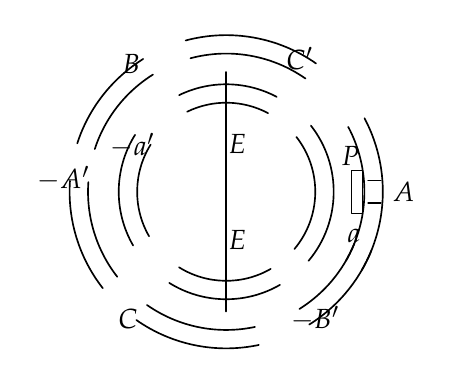
\begin{tikzpicture}[scale=0.78, line cap=round, line join=round]
  \def\rA{2.55}
  \def\rB{2.25}
  \def\rC{1.75}
  \def\rD{1.45}
  \draw[line width=0.55pt] (0,-1.95) -- (0,1.95);
  \node at (0.18,0.78) {$E$};
  \node at (0.18,-0.78) {$E$};

  \foreach \ra/\rb/\sa/\ea in {
    \rA/\rB/-30/28,
    \rA/\rB/55/105,
    \rA/\rB/122/162,
    \rA/\rB/176/218,
    \rA/\rB/235/282,
    \rA/\rB/302/338,
    \rC/\rD/-40/38,
    \rC/\rD/62/116,
    \rC/\rD/148/210,
    \rC/\rD/238/300
  }{
    \draw[line width=0.6pt] (\sa:\ra) arc[start angle=\sa,end angle=\ea,radius=\ra];
    \draw[line width=0.6pt] (\sa:\rb) arc[start angle=\sa,end angle=\ea,radius=\rb];
  }

  \draw[line width=0.5pt] (2.04,-0.35) rectangle (2.22,0.35);
  \draw[line width=0.5pt] (2.31,-0.18) -- (2.52,-0.18);
  \draw[line width=0.5pt] (2.31,0.18) -- (2.52,0.18);
  \node[right] at (2.55,0) {$A$};
  \node at (2.02,0.58) {$P$};
  \node at (2.08,-0.72) {$a$};

  \node at (-1.55,2.08) {$B$};
  \node at (1.20,2.17) {$C'$};
  \node at (-2.65,0.22) {$-A'$};
  \node at (-1.52,0.75) {$-a'$};
  \node at (-1.60,-2.08) {$C$};
  \node at (1.45,-2.07) {$-B'$};
\end{tikzpicture}

Fig. 17.
\end{center}

Now we have shewn that whenever this occurs there is a loss of energy,
and therefore the whole work employed in turning the machine is not
converted into electrification in an available form, but part is spent in
producing the heat and noise of electric sparks.

I have therefore thought it desirable to shew how an electrical machine
may be constructed which is not subject to this loss of efficiency. I do
not propose it as a useful form of machine, but as an example of the
method by which the contrivance called in heat-engines a regenerator may
be applied to an electrical machine to prevent loss of work.

In the figure let $A$, $B$, $C$, $A'$, $B'$, $C'$ represent hollow fixed
conductors, so arranged that the carrier $P$ passes in succession within
each of them. Of these $A$, $A'$ and $B$, $B'$ nearly surround the

\clearpage

carrier when it is at the middle point of its passage, but $C$, $C'$ do not
cover it so much.

We shall suppose $A$, $B$, $C$ to be connected with a Leyden jar
of great capacity at potential $V$, and $A'$, $B'$, $C'$ to be connected
with another jar at potential $-V'$.

$P$ is one of the carriers moving in a circle from $A$ to $C'$, \&c.,
and touching in its course certain springs, of which $a$ and $a'$ are
connected with $A$ and $A'$ respectively, and $e$, $e'$ are connected with
the earth.

Let us suppose that when the carrier $P$ is in the middle of $A$
the coefficient of induction between $P$ and $A$ is $-A$. The capacity
of $P$ in this position is greater than $A$, since it is not completely
surrounded by the receiver $A$. Let it be $A+a$.

Then if the potential of $P$ is $U$, and that of $A$, $V$, the charge
on $P$ will be
\[
(A+a)U-AV.
\]

Now let $P$ be in contact with the spring $a$ when in the middle
of the receiver $A$, then the potential of $P$ is $V$, the same as that
of $A$, and its charge is therefore $aV$.

If $P$ now leaves the spring $a$ it carries with it the charge $aV$.
As $P$ leaves $A$ its potential diminishes, and it diminishes still more
when it comes within the influence of $C'$, which is negatively
electrified.

If when $P$ comes within $C$ its coefficient of induction on $C$ is
$-C'$, and its capacity is $C'+c'$, then, if $U$ is the potential of $P$
the charge on $P$ is
\[
(C'+c')U+C'V'=aV.
\]
If
\[
C'V'=aV,
\]
then at this point $U$ the potential of $P$ will be reduced to zero.
Let $P$ at this point come in contact with the spring $e'$ which is
connected with the earth. Since the potential of $P$ is equal to that
of the spring there will be no spark at contact.

This conductor $C'$, by which the carrier is enabled to be connected
to earth without a spark, answers to the contrivance called a
regenerator in heat-engines. We shall therefore call it a Regenerator.

Now let $P$ move on, still in contact with the earth-spring $e'$, till
it comes into the middle of the inductor $B$, the potential of which
is $V$. If $-B$ is the coefficient of induction between $P$ and $B$ at
this point, then, since $U=0$ the charge on $P$ will be $-BV$.

When $P$ moves away from the earth-spring it carries this charge
with it. As it moves out of the positive inductor $B$ towards the

\clearpage

negative receiver $A'$ its potential will be increasingly negative. At
the middle of $A'$, if it retained its charge, its potential would be
\[
-\frac{A'V'+BV}{A'+a'},
\]
and if $BV$ is greater than $a'V'$ its numerical value will be greater
than that of $V'$. Hence there is some point before $P$ reaches the
middle of $A'$ where its potential is $-V'$. At this point let it come
in contact with the negative receiver-spring $a'$. There will be no
spark since the two bodies are at the same potential. Let $P$ move on
to the middle of $A'$, still in contact with the spring, and therefore
at the same potential with $A'$. During this motion it communicates
a negative charge to $A'$. At the middle of $A'$ it leaves the spring
and carries away a charge $-a'V'$ towards the positive regenerator
$C$, where its potential is reduced to zero and it touches the
earth-spring $e$. It then slides along the earth-spring into the negative
inductor $B'$, during which motion it acquires a positive charge
$B'V'$ which it finally communicates to the positive receiver $A$, and
the cycle of operations is repeated.

During this cycle the positive receiver has lost a charge $aV$ and
gained a charge $B'V'$. Hence the total gain of positive electricity is
\[
B'V'-aV.
\]
Similarly the total gain of negative electricity is $BV-a'V'$.

By making the inductors so as to be as close to the surface of
the carrier as is consistent with insulation, $B$ and $B'$ may be made
large, and by making the receivers so as nearly to surround the
carrier when it is within them, $a$ and $a'$ may be made very small,
and then the charges of both the Leyden jars will be increased in
every revolution.

The conditions to be fulfilled by the regenerators are
\[
C'V'=aV,\qquad \hbox{and}\qquad CV=a'V'.
\]

Since $a$ and $a'$ are small the regenerators do not require to be
either large or very close to the carriers.

\section*{\textit{On Electrometers and Electroscopes.}}

214.] An electrometer is an instrument by means of which
electrical charges or electrical potentials may be measured.
Instruments by means of which the existence of electric charges or
of differences of potential may be indicated, but which are not
capable of affording numerical measures, are called Electroscopes.

An electroscope if sufficiently sensible may be used in electrical
measurements, provided we can make the measurement depend on

\clearpage

the absence of electrification. For instance, if we have two charged
bodies $A$ and $B$ we may use the method described in Chapter I to
determine which body has the greater charge. Let the body $A$ be
carried by an insulating support into the interior of an insulated
closed vessel $C$. Let $C$ be connected to earth and again insulated.
There will then be no external electrification on $C$. Now let $A$
be removed, and $B$ introduced into the interior of $C$, and the
electrification of $C$ tested by an electroscope. If the charge of $B$
is equal to that of $A$ there will be no electrification, but if it is
greater or less there will be electrification of the same kind as that
of $B$, or the opposite kind.

Methods of this kind, in which the thing to be observed is the
non-existence of some phenomenon, are called \textit{null} or \textit{zero}
methods. They require only an instrument capable of detecting the
existence of the phenomenon.

In another class of instruments for the registration of phenomena
the instrument may be depended upon to give always the same
indication for the same value of the quantity to be registered, but
the readings of the scale of the instrument are not proportional
to the values of the quantity, and the relation between these
readings and the corresponding value is unknown, except that the
one is some continuous function of the other. Several electrometers
depending on the mutual repulsion of parts of the instrument which
are similarly electrified are of this class. The use of such instruments
is to register phenomena, not to measure them. Instead of the true
values of the quantity to be measured, a series of numbers is obtained,
which may be used afterwards to determine these values when the scale
of the instrument has been properly investigated and tabulated.

In a still higher class of instruments the scale readings are
proportional to the quantity to be measured, so that all that is
required for the complete measurement of the quantity is a knowledge
of the coefficient by which the scale readings must be multiplied to
obtain the true value of the quantity.

Instruments so constructed that they contain within themselves
the means of independently determining the true values of quantities
are called Absolute Instruments.

\section*{\textit{Coulomb's Torsion Balance.}}

215.] A great number of the experiments by which Coulomb

\clearpage

established the fundamental laws of electricity were made by measuring
the force between two small spheres charged with electricity, one of
which was fixed while the other was held in equilibrium by two forces,
the electrical action between the spheres, and the torsional elasticity
of a glass fibre or metal wire. See Art. 38.

The balance of torsion consists of a horizontal arm of gum-lac,
suspended by a fine wire or glass fibre, and carrying at one end a
little sphere of elder pith, smoothly gilt. The suspension wire is
fastened above to the vertical axis of an arm which can be moved
round a horizontal graduated circle, so as to twist the upper end
of the wire about its own axis any number of degrees.

The whole of this apparatus is enclosed in a case. Another little
sphere is so mounted on an insulating stem that it can be charged
and introduced into the case through a hole, and brought so that
its centre coincides with a definite point in the horizontal circle
described by the suspended sphere. The position of the suspended
sphere is ascertained by means of a graduated circle engraved on
the cylindrical glass case of the instrument.

Now suppose both spheres charged, and the suspended sphere
in equilibrium in a known position such that the torsion-arm makes
an angle $\theta$ with the radius through the centre of the fixed sphere.
The distance of the centres is then $2a\sin\frac{1}{2}\theta$, where $a$
is the radius of the torsion-arm, and if $F$ is the force between the
spheres the moment of this force about the axis of torsion is
$Fa\cos\frac{1}{2}\theta$.

Let both spheres be completely discharged, and let the torsion-arm
now be in equilibrium at an angle $\phi$ with the radius through
the fixed sphere.

Then the angle through which the electrical force twisted the
torsion-arm must have been $\theta-\phi$, and if $M$ is the moment of
the torsional elasticity of the fibre, we shall have the equation
\[
Fa\cos\frac{1}{2}\theta = M(\theta-\phi).
\]
Hence, if we can ascertain $M$, we can determine $F$, the actual
force between the spheres at the distance $2a\sin\frac{1}{2}\theta$.

To find $M$, the moment of torsion, let $I$ be the moment of inertia
of the torsion-arm, and $T$ the time of a double vibration of the arm
under the action of the torsional elasticity, then
\[
M=\frac{1}{4\pi^2}IT^2.
\]

In all electrometers it is of the greatest importance to know
what force we are measuring. The force acting on the suspended

\clearpage

sphere is due partly to the direct action of the fixed sphere, but
partly also to the electrification, if any, of the sides of the case.

If the case is made of glass it is impossible to determine the
electrification of its surface otherwise than by very difficult
measurements at every point. If, however, either the case is made
of metal, or if a metallic case which almost completely encloses the
apparatus is placed as a screen between the spheres and the glass
case, the electrification of the inside of the metal screen will depend
entirely on that of the spheres, and the electrification of the glass
case will have no influence on the spheres. In this way we may
avoid any indefiniteness due to the action of the case.

To illustrate this by an example in which we can calculate all
the effects, let us suppose that the case is a sphere of radius $b$,
that the centre of motion of the torsion-arm coincides with the
centre of the sphere and that its radius is $a$; that the charges on
the two spheres are $E$ and $E_1$, and that the angle between their
positions is $\theta$; that the fixed sphere is at a distance $a_1$ from
the centre, and that $r$ is the distance between the two small spheres.

Neglecting for the present the effect of induction on the distribution
of electricity on the small spheres, the force between them will be
a repulsion
\[
=\frac{EE_1}{r^2},
\]
and the moment of this force round a vertical axis through the
centre will be
\[
\frac{EE_1aa_1\sin\theta}{r^3}.
\]

The image of $E_1$ due to the spherical surface of the case is a point
in the same radius at a distance $\frac{b^2}{a_1}$ with a charge
$-E_1\frac{b}{a_1}$, and the moment of the attraction between $E$
and this image about the axis of suspension is
\[
\begin{split}
EE_1\frac{b}{a_1}
&\frac{a\frac{b^2}{a_1}\sin\theta}
{\left\{a^2-2\frac{ab^2}{a_1}\cos\theta+\frac{b^4}{a_1^2}\right\}^{\frac{3}{2}}}
\\
={}&EE_1
\frac{aa_1\sin\theta}
{b^3\left\{1-2\frac{aa_1}{b^2}\cos\theta+\frac{a^2a_1^2}{b^4}\right\}^{\frac{3}{2}}}.
\end{split}
\]

If $b$, the radius of the spherical case, is large compared with $a$

\clearpage

and $a_1$, the distances of the spheres from the centre, we may neglect
the second and third terms of the factor in the denominator. The
whole moment tending to turn the torsion-arm may then be written
\[
EE_1aa_1\sin\theta\left\{\frac{1}{r^3}-\frac{1}{b^3}\right\}
=M(\theta-\phi).
\]

\section*{\textit{Electrometers for the Measurement of Potentials.}}

216.] In all electrometers the moveable part is a body charged
with electricity, and its potential is different from that of certain
of the fixed parts round it. When, as in Coulomb's method, an
insulated body having a certain charge is used, it is the charge
which is the direct object of measurement. We may, however,
connect the balls of Coulomb's electrometer, by means of fine wires,
with different conductors. The charges of the balls will then depend
on the values of the potentials of these conductors and on the
potential of the case of the instrument. The charge on each ball
will be approximately equal to its radius multiplied by the excess
of its potential over that of the case of the instrument, provided
the radii of the balls are small compared with their distances from
each other and from the sides or opening of the case.

Coulomb's form of apparatus, however, is not well adapted for
measurements of this kind, owing to the smallness of the force
between spheres at the proper distances when the difference of
potentials is small. A more convenient form is that of the Attracted
Disk Electrometer. The first electrometers on this principle were
constructed by Sir W. Snow Harris\setcounter{footnote}{0}\footnote{\textit{Phil. Trans.} 1834.}
They have since been brought to great perfection, both in theory
and construction, by Sir W. Thomson\footnote{See an excellent report
on Electrometers by Sir W. Thomson. \textit{Report of the British
Association}, Dundee, 1867.}.

When two disks at different potentials are brought face to face
with a small interval between them there will be a nearly uniform
electrification on the opposite faces and very little electrification
on the backs of the disks, provided there are no other conductors
or electrified bodies in the neighbourhood. The charge on the
positive disk will be approximately proportional to its area, and to
the difference of potentials of the disks, and inversely as the distance
between them. Hence, by making the areas of the disks large

\clearpage

and the distance between them small, a small difference of potential
may give rise to a measurable force of attraction.

The mathematical theory of the distribution of electricity over
two disks thus arranged is given at Art. 202, but since it is impossible
to make the case of the apparatus so large that we may suppose the
disks insulated in an infinite space, the indications of the instrument
in this form are not easily interpreted numerically.

217.] The addition of the guard-ring to the attracted disk is one
of the chief improvements which Sir W. Thomson has made on the
apparatus.

Instead of suspending the whole of one of the disks and determining
the force acting upon it, a central portion of the disk is separated
from the rest to form the attracted disk, and the outer ring forming
the remainder of the disk is fixed. In this way the force is measured
only on that part of the disk where it is most regular, and the want
of uniformity of the electrification near the

\begin{center}
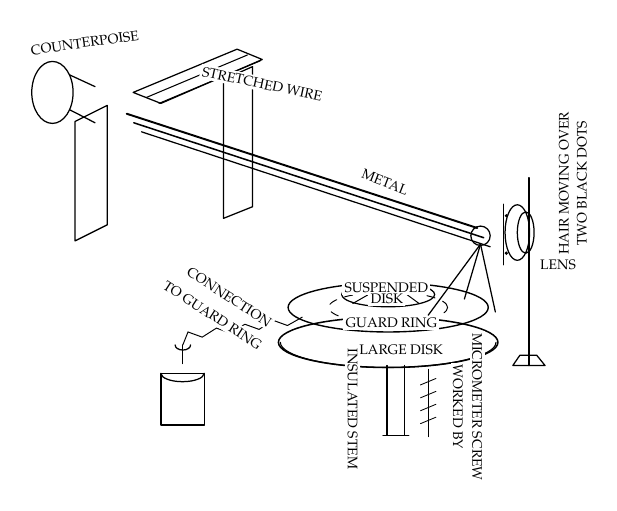
\begin{tikzpicture}[scale=0.82, line cap=round, line join=round,
  every node/.style={font=\fontsize{5}{5}\selectfont, inner sep=0.8pt}]
  % Counterpoise, standards, and stretched-wire support.
  \draw[line width=0.45pt] (-5.20,2.15) ellipse (0.32 and 0.48);
  \draw[line width=0.45pt] (-4.93,1.88) -- (-4.54,1.68);
  \draw[line width=0.45pt] (-4.93,2.42) -- (-4.54,2.24);
  \draw[line width=0.45pt] (-4.85,-0.15) -- (-4.85,1.70) -- (-4.35,1.95) -- (-4.35,0.10) -- cycle;
  \draw[line width=0.45pt] (-2.55,0.20) -- (-2.55,2.35) -- (-2.10,2.55) -- (-2.10,0.38) -- cycle;
  \node[rotate=8, fill=white] at (-4.70,2.92) {COUNTERPOISE};

  \draw[line width=0.45pt] (-3.95,2.15) -- (-2.34,2.82) -- (-1.95,2.66) -- (-3.52,1.98) -- cycle;
  \draw[line width=0.38pt] (-3.75,2.07) -- (-2.18,2.73);
  \draw[line width=0.38pt] (-3.55,1.98) -- (-1.98,2.64);
  \node[rotate=-12, fill=white] at (-1.95,2.28) {STRETCHED WIRE};

  % Metal balance beam and suspension.
  \draw[line width=0.7pt] (-4.05,1.82) -- (1.38,0.05);
  \draw[line width=0.55pt] (-3.94,1.68) -- (1.48,-0.10);
  \draw[line width=0.45pt] (-3.82,1.54) -- (1.58,-0.24);
  \node[rotate=-21, fill=white] at (-0.05,0.76) {METAL};
  \draw[line width=0.45pt] (1.43,-0.07) circle (0.15);
  \draw[line width=0.45pt] (1.43,-0.20) -- (0.62,-1.30);
  \draw[line width=0.45pt] (1.43,-0.20) -- (1.66,-1.25);
  \draw[line width=0.45pt] (1.43,-0.20) -- (1.18,-1.05);

  % Lens and fiducial hair/dots.
  \draw[line width=0.45pt] (2.18,-2.08) -- (2.18,0.83);
  \draw[line width=0.45pt] (2.00,-0.02) ellipse (0.19 and 0.43);
  \draw[line width=0.45pt] (2.13,-0.02) ellipse (0.13 and 0.32);
  \draw[line width=0.45pt] (1.93,-2.08) -- (2.43,-2.08) -- (2.30,-1.92) -- (2.04,-1.92) -- cycle;
  \fill (1.83,0.24) circle (0.028);
  \fill (1.83,-0.34) circle (0.028);
  \draw[line width=0.35pt] (1.78,-0.52) -- (1.78,0.42);
  \node[rotate=90, fill=white] at (2.72,0.74) {HAIR MOVING OVER};
  \node[rotate=90, fill=white] at (3.00,0.74) {TWO BLACK DOTS};
  \node[fill=white] at (2.63,-0.52) {LENS};

  % Guard-ring apparatus: large disk, guard ring, suspended disk.
  \draw[line width=0.55pt] (0,-1.72) ellipse (1.70 and 0.39);
  \draw[line width=0.4pt] (-1.67,-1.72) arc[start angle=180,end angle=360,x radius=1.67,y radius=0.39];
  \draw[line width=0.5pt] (0,-1.18) ellipse (1.55 and 0.38);
  \draw[dashed,line width=0.35pt] (0,-1.18) ellipse (0.92 and 0.24);
  \draw[line width=0.45pt] (0,-0.98) ellipse (0.72 and 0.19);
  \draw[line width=0.35pt] (-0.55,-1.12) -- (-0.20,-0.92);
  \draw[line width=0.35pt] (0.48,-1.12) -- (0.18,-0.90);
  \node[fill=white] at (-0.03,-0.88) {SUSPENDED};
  \node[fill=white] at (-0.02,-1.05) {DISK};
  \node[fill=white] at (0.05,-1.42) {GUARD RING};
  \node[fill=white] at (0.20,-1.84) {LARGE DISK};

  % Insulated stem and micrometer screw beneath the large disk.
  \draw[line width=0.45pt] (-0.02,-2.08) -- (-0.02,-3.16);
  \draw[line width=0.45pt] (0.25,-2.08) -- (0.25,-3.16);
  \draw[line width=0.45pt] (-0.08,-3.16) -- (0.32,-3.16);
  \draw[line width=0.35pt] (0.62,-2.14) -- (0.62,-3.18);
  \foreach \y in {-2.98,-2.78,-2.58,-2.38} {
    \draw[line width=0.3pt] (0.50,\y) -- (0.74,\y+0.10);
  }
  \node[rotate=-90, fill=white] at (-0.55,-2.75) {INSULATED STEM};
  \node[rotate=-90, fill=white] at (1.08,-2.72) {WORKED BY};
  \node[rotate=-90, fill=white] at (1.38,-2.72) {MICROMETER SCREW};

  % External connection to the guard ring.
  \draw[line width=0.35pt] (-1.33,-1.33)
    -- (-1.56,-1.46) -- (-1.78,-1.38) -- (-2.00,-1.52)
    -- (-2.22,-1.44) -- (-2.44,-1.58) -- (-2.66,-1.50)
    -- (-2.88,-1.64) -- (-3.10,-1.56);
  \node[rotate=-33, fill=white] at (-2.46,-1.02) {CONNECTION};
  \node[rotate=-33, fill=white] at (-2.72,-1.30) {TO GUARD RING};
  \draw[line width=0.45pt] (-3.52,-3.00) rectangle (-2.85,-2.20);
  \draw[line width=0.45pt] (-3.52,-2.20) arc[start angle=180,end angle=360,x radius=0.335,y radius=0.13];
  \draw[line width=0.45pt] (-3.18,-2.05) -- (-3.18,-1.76);
  \draw[line width=0.45pt] (-3.30,-1.76) arc[start angle=180,end angle=360,x radius=0.12,y radius=0.08];
  \draw[line width=0.35pt] (-3.18,-1.76) -- (-3.10,-1.56);
\end{tikzpicture}

Fig. 18.
\end{center}

edge is of no importance, as it occurs on the guard-ring and not
on the suspended part of the disk.

Besides this, by connecting the guard-ring with a metal case
surrounding the back of the attracted disk and all its suspending
apparatus, the electrification of the back of the disk is rendered

\clearpage

impossible, for it is part of the inner surface of a closed hollow conductor all at the same potential.

Thomson s Absolute Electrometer therefore consists essentially of two parallel plates at different potentials, one of which ismade so that a certain area, no part of which isnear the edge of the plate, is moveable under the action of electric force. To fix our ideas we may suppose the attracted disk and guard-ring uppermost. The fixed disk is horizontal, and is mounted on an insulating stem which has a measurable vertical motion given to it by means of a micrometer screw. The guard-ring is at least as large as the fixed disk ; its lower surface is truly plane and parallel to the fixed disk. A delicate balance is erected on the guard-ring to which is suspended a light moveable disk which almost fills the circular aperture in the guard-ring without rubbing against its sides. The lower surface of the suspended disk must be truly plane, and we must have the means of knowing when itsplane coincides with that of the lower surface of the guard-ring, so as to form a single plane interrupted only by the narrow interval between the disk and its guard-ring.

For this purpose the lower disk is screwed up till it is in contact with the guard-ring, and the suspended disk is allowed to rest upon the lower disk, so that its lower surface is in the same plane as that of the guard-ring. Its position with respect to the guardring is then ascertained by means of a system of fiducial marks. Sir W. Thomson generally uses for this purpose a black hair attached to the moveable part. This hair moves up or down just in front of two black dots on a white enamelled ground and is viewed along with these dots by means of a piano convex lens with the plane side next the eye. If the hair as seen through the lens appears straight and bisects the interval between the black dots it is said to be in its sighted position, and indicates that the sus pended disk with which itmoves is in its proper position as regards height. The horizontality of the suspended disk may be tested by comparing the reflexion of part of any object from its upper surface with that of the remainder of the same object from the upper surface of the guard-ring.

The balance is then arranged so that when a known weight is placed on the centre of the suspended disk it is in equilibrium in its sighted position, the whole apparatus being freed from electrification by putting every part in metallic communication. A metal case is placed over the guard-ring so as to enclose the

\end{document}
